
\documentclass[onehalfspacing,reservepages,10pt]{sjvanschaik-thesis}

\usepackage[english]{babel}
\usepackage[utf8]{inputenc}
\usepackage{graphicx}
\usepackage{flushend}
\usepackage{palatino}
\usepackage{enumitem}
\usepackage{wrapfig}
\usepackage{epigraph}
\usepackage{subfig}
\usepackage[table,xcdraw,dvipsnames]{xcolor}
\usepackage{multirow}

\usepackage[noend]{algpseudocode}
\usepackage{algorithm}


\makeatletter
\renewcommand{\@chapapp}{}% Not necessary...
\newenvironment{chapquote}[2][2em]
  {\setlength{\@tempdima}{#1}%
   \def\chapquote@author{#2}%
   \parshape 1 \@tempdima \dimexpr\textwidth-2\@tempdima\relax%
   \itshape}
  {\par\normalfont\hfill--\ \chapquote@author\hspace*{\@tempdima}\par\bigskip}
\makeatother
\newcommand{\lt}{<}
\newcommand{\gt}{>}

\ThesisAuthor{Eamonn J. Maguire}
\ThesisCollege{St. Anne's College}
\ThesisTitle{Systematising Glyph Design for Visualization}
\ThesisTerm{Michaelmas}
\ThesisYear{2014}

% TODO:
\ThesisKeywords{{visualization}; {compression}}

\begin{document}

\frontmatter
\maketitle

\begin{romanpages}
\ThesisAbstract{%
The digitalisation of information now affects most fields of human activity.
From the social sciences to biology to physics, the volume, velocity, and variety of data exhibit exponential growth trends.
With such rates of expansion, efforts to understand and make sense of datasets of such scale, however driven and directed, progress only at an incremental pace.
The challenges are significant.
For instance, the ability to display an ever growing amount of data is physically and naturally bound by the dimensions of the average sized display.
A synergistic interplay between statistical analysis and visualisation approaches outlines a path for significant advances in the field of data exploration.
We can turn to statistics to provide principled guidance for prioritisation of information to display.
Using statistical results, and combining knowledge from the cognitive sciences, visual techniques can be used to highlight salient data attributes.

The purpose of this thesis is to explore the link between computer science, statistics, visualization, and the cognitive sciences, to define and develop more systematic approaches towards the design of glyphs.

Glyphs represent the variables of multivariate data records by mapping those variables to one or more visual channels (\eg, colour, shape, and texture).
They offer a unique, compact solution to the presentation of a large amount of multivariate information.
However, composing a meaningful, interpretable, and learnable glyph can pose a number of problems.
The first of these problems exist in the subjectivity involved in the process of data to visual channel mapping, and in the organisation of those visual channels to form the overall glyph.
Our first contribution outlines a computational technique to help systematise many of these otherwise subjective elements of the glyph design process.

For visual information compression, common patterns (motifs) in time series or graph data for example, may be replaced with more compact, visual representations.
Glyph-based techniques can provide such representations that can help users find common patterns more quickly, and at the same time, bring attention to anomalous areas of the data.
However, replacing any data with a glyph is not going to make tasks such as visual search easier.
A key problem is the selection of semantically meaningful motifs with the potential to compress large amounts of information.
A second contribution of this thesis is a computational process for systematic design of such glyph libraries and their subsequent glyphs.

A further problem in the glyph design process is in their evaluation.
Evaluation is typically a time-consuming, highly subjective process.
Moreover, domain experts are not always plentiful, therefore obtaining statistically significant evaluation results is often difficult.
A final contribution of this work is to investigate if there are areas of evaluation that can be performed  computationally.
}
\Abstract

\begin{dedication}
Dedicated to my Mum.
\end{dedication}

\begin{acknowledgements}

\noindent I'm in so much debt to many people who have been part of this enjoyable journey, but first and foremost I would like to thank my supervisors Prof. Min Chen, Prof. Jim Davies and Dr. Susanna-Assunta Sansone. 


To Min Chen who took me as a raw DPhil student and through his support, patience, guidance, and endless energy has helped guide me through the entire process. 
It has been a great pleasure to work with someone held in such high esteem by the visualization community and I am so fortunate to have been given the chance to conduct my DPhil with him.


To Susanna-Assunta Sansone who has given me the freedom to pursue a DPhil whilst conducting research and the Oxford e-Research Centre (OeRC) for supporting this process. 
We have worked together for six years now, and I have enjoyed being in her growing group and seeing things go from strength to strength.

To Philippe Rocca-Serra who has also put up with me for six years now, interspersed with my delightfully accurate French accent. 
Philippe is a great friend who has been a tremendous support through all stages of this journey, in particular the more difficult ones. 

To Annapaola Santarsiero who has dealt with the many late nights and weekend work for three years whilst always being supportive.
Annapaola even agreed to marry me when I proposed during the writing up process!

Additionally, I owe a great deal to my incredibly talented friends and colleagues at the OeRC who have made my time in Oxford so great.
Their knowledge, passion, friendliness, and availability to share their knowledge has been amazing.
In particular I wish to thank Alejandra González-Beltrán, Simon Walton, Alfie Abdul-Rahman, Brian Duffy, Endre Lászió, Piotr Łopatka, Ramon Granell, Raz Lakhoo, Stef Salvini, Istvan Reguly, Ségolène Tarte (who also endured my French accents), Milo Thurston, Neil Caithness, Bas van Schaik, Kay Sutton, Ross McCartney, Clem Harris, and David DeRoure. 

Finally to my great network of friends in Oxford and beyond who have all in some way played a part in my journey, including Tommy Barr, Ryan McCrea, David Close, Liam Kelly, Matt Brinklow, Devan Govender, James Malone, Will McClaren, Rasmus Wissman, Sam Whitehead, Chris Boddy, Dan Short, Ian Robertson, Caterina Doglioni, and so many more!

I would also like to thank and remember the contributions of Professor Matthew Ward who researched glyphs extensively and contributed a large amount of knowledge in the direction of glyph-based visualization.
Professor Ward was to present with Dr. Rita Borgo, Prof. Min Chen, and Prof. Sine McDougall at the glyph tutorial at VIS 2014 in Paris, but sadly passed away in October 2014.

\end{acknowledgements}
   
\begin{publications}

\noindent\textbf{Publications}

\noindent The work conducted in this thesis has led to the following publications. \\

\noindent \textbf{E. Maguire}‚ P. Rocca-Serra‚ S.-A. Sansone‚ J. Davies, and M. Chen. \emph{Taxonomy-based Glyph Design - with a Case Study on Visualizing Workflows of Biological Experiments}. In IEEE Transactions on Visualization and Computer Graphics, Pages 2603-2612, Volume 18 (2012).\\

\noindent R. Borgo, J. Kehrer, D.H.S. Chung, \textbf{E. Maguire}, R. S. Laramee, H. Hauser, M. Ward, and M. Chen. \emph{Glyph-based visualization: Foundations, design guidelines, techniques and applications}. In Eurographics State of the Art Reports, EG STARs (2013), Pages 39-63.\\

\noindent A. Abdul-Rahman, J. Lein, K. Coles, \textbf{E. Maguire}, M. Meyer, M. Wynne, C. R. Johnson, A. Trefethen, and M. Chen. \emph{Rule-based Visual Mappings - with a Case Study on Poetry Visualization}. In Computer Graphics Forum, Pages 381-390, Volume 32 (2013).\\

\noindent \textbf{E. Maguire}‚ P. Rocca-Serra‚ S.-A. Sansone‚ J. Davies, and M. Chen. \emph{Visual Compression of Workflow Visualizations with Automated Detection of Macro Motifs}. In IEEE Transactions on Visualization and Computer Graphics, Pages 2576-2585, Volume 19 (2013).\\

\noindent A. Abdul-Rahman‚ \textbf{E. Maguire} and M. Chen. \emph{Comparing Three Designs of Macro-Glyphs for Poetry Visualization}. In Proceedings of EuroVis 2014‚ Short Paper (2014).\\

\noindent \textbf{E. Maguire}‚ P. Rocca-Serra‚ S.-A. Sansone, and M. Chen. \emph{Redesigning the Sequence Logo with Glyph-based Approaches to Aid Interpretation}. In Proceedings of EuroVis 2014‚ Short Paper (2014).\\

\noindent S. Walton, \textbf{E. Maguire}‚ and M. Chen. \emph{Multiple Queries with Conditional Attributes (QCATs) for Anomaly Detection and Visualization}. In Proceedings of the Eleventh Workshop on Visualization for Cyber Security, VizSec 2014.\\

\noindent\textbf{Tutorials}\\

\noindent \emph{Glyph-based visualization tutorial} - presented at IEEE VIS 2014. Co-organized with R. Borgo and M. Chen. 

\end{publications}
   

%set the number of sectioning levels that get number and appear in the contents
\setcounter{secnumdepth}{3}
\setcounter{tocdepth}{3}

{\fontsize{12pt}{14pt}\selectfont\tableofcontents} 

\end{romanpages}

\mainmatter

%\chapter{My Chapter}
%\blindtext

\chapter{Introduction}
\label{chap:introduction}

In an article published in 2002, Matt Ward stated that data sizes were exploding \cite{ward02}.
Since then, the rate of data growth has not relented.
Facebook, Twitter, LinkedIn, and Google Plus, all of which did not exist in 2002, contribute huge amounts of information to government departments, marketers, and social scientists.
The democratisation of DNA sequencing technology combined with a scientific need to bring together many different data sources in to their analyses (\eg, RNA, proteomic, metabolomic, and clinical chemistry data) has pushed the biological sciences into a more data-centric domain.
Since 2008, physicists can now get their hands and algorithms on over 20 petabytes of information every year from the large hadron collider at CERN.
By bringing together lots of information from different sources, it is commonplace for a data record to have anything from tens to thousands of quantitative and qualitative data variables (termed multivariate data) \cite{ward02}.

So how does one deal with such data and interpret it?
Statistical techniques are effective in the detection of trends and outliers in data where there is a pre-existing model of what is expected.
However, they are not so effective in the detection of trends and outliers in data when no such model exists.
The human perceptual system is incredibly powerful at finding patterns or outliers that statistical techniques may miss.
When no model is yet known or unavailable, or when uncertainty exists on an underlying model, visualization can take advantage of the human perceptual system to help users in a number of tasks, including:
\begin{enumerate}
\item observation of trends and outliers;
\item creating connections between data and past experience, knowledge, and intuition;
\item visual generation and evaluation of hypotheses;
\item monitoring the correctness and performance of computational models; and 
\item effective communication with others.
\end{enumerate}

\begin{figure}[t!]
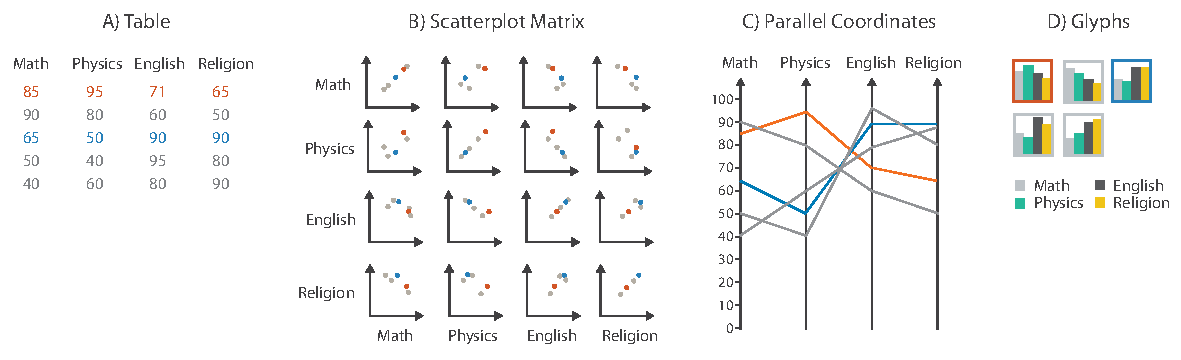
\includegraphics[width=\textwidth]{images/introduction/multivariate_vis}
\caption{Techniques for multivariate data exploration include: A) tables; B) scatter plot matrices (SPLOMS); C) parallel coordinate plots; and D) glyph-based visualization.}
\label{fig:multivariate_vis}
\end{figure}

Multivariate data visualization is a class of visualization techniques that deal with the presentation of many data record attributes at once.
Four primary multivariate data visualization techniques displayed in Figure \ref{fig:multivariate_vis} are:

\begin{enumerate}
\item \textbf{Data Tables} (Figure \ref{fig:multivariate_vis} A) are the simplest and most pervasive form of visualization.
There are many limitations to tables over more graphical visualization techniques generally around scalability (you can only view a limited number of rows at a time), and trend/outlier identification problems (it is hard to see large scale trends in a table);

\item \textbf{Scatter plot matrices (SPLOMS)} (Figure \ref{fig:multivariate_vis} B) where each dimension of a record is plotted against other dimensions \cite{Elmqvist2008Scatter} as an individual scatter plot.
This technique suffers in that $N^2$ plots are required where $N$ is the number of dimensions.
So while this technique is effective for a small number of dimensions, its capabilities diminish as the number of dimensions grow; 

\item \textbf{Parallel coordinate plots} (Figure \ref{fig:multivariate_vis} C) encode each variable/dimension of a data record as an axis with a line passing through each axis at the point given by the data record.
A full review of parallel coordinates can be found in a STAR from Heinrich and Weiskopf \cite{heinrich2012state}; and

\item \textbf{Glyph-based visualization} (Figure \ref{fig:multivariate_vis} D) uses visual items (termed glyphs) to encode data attributes using a number of visual channels (\eg, colour, shape, size, position, etc.).
These glyphs can then be positioned independently in 2D or 3D space to form the overall visualization.
\end{enumerate}


\section{Glyph-based Visualization Challenges}
While tables, SPLOMs and parallel coordinate plots can be deployed relatively easily, \emph{effective} glyph-based solutions are generally more difficult to implement.
Glyph-based visualization is a powerful technique, offering an advantage over other multivariate data visualization techniques in their ability to preserve spatial information.
However, their implementation is not straightforward and a number of challenges exist within information visualization (largely 2D) and scientific visualization (largely 3D).
Drawing from the State of the Art Report (STAR) on glyph-based visualization from Borgo \etal \cite{Borgo:2013:EG}, and Matt Ward's paper on ``Multivariate Data Glyphs: Principles and Practice'', the following challenges can be extrapolated:


\begin{enumerate}
\item \textbf{Technical Challenges}:
	\begin{enumerate}
		\item \textbf{Challenge 1} - \emph{Glyph Placement} concerns how glyphs are arranged spatially in 2D or 3D scenes.
		Position is an important visual channel, therefore ensuring glyphs are displayed in the right position is a key problem in many domains.
		
		Matt Ward's excellent survey on glyph placement provides a great overview of a number of strategies for glyph placement that includes data- and structure-driven techniques \cite{ward02}.
		Ropinski \cite{ropinski11} added a further strategy for medical data, named feature-driven glyph placement which places glyphs on particular features of the underlying data.
		Borgo \etal \cite{Borgo:2013:EG} also added user-driven glyph placement as a categorisation.
		Glyph placement remains a problem within the visualization community due to problems with occlusion for example.
		
		\item \textbf{Challenge 2} - \emph{Data Ordering} considers how data records can be ordered or have sets of variables grouped to highlight specific trends or interesting parts of the data\cite{ward08}.
		The ordering of the underlying data can influence how particular features of the data are interpreted during analysis and is very much task dependent.
		For example, if a user is using a glyph-based visualization to gain an overview of how much customers have spent over the past year, having randomly ordered monthly totals is not going to be as useful as having the months arranged naturally from January to December.
		
		\item \textbf{Challenge 3} - \emph{Glyph-based Visual Compression} is a technique that uses glyphs to reduce the amount of visual space taken up in a display by common patterns/motifs.
		A key challenge in this technique is determining which parts of the data are not only common, but will also visually compress the most space.
		Additionally, instead of ad-hoc compressions of data, a further challenge would be in creating glyph libraries to be used across a domain to consistently represent common features in their data.
		
	\end{enumerate}
\item \textbf{Design Challenges}:
	\begin{enumerate}
			\item \textbf{Challenge 4} -  \emph{Data to Visual Mapping} relates to how particular data variables are mapped to colour, shape, size, and texture for example (called visual channels).
			Mappings can vary depending on the type of the data variable (\eg, categorical or quantitative) with not all visual channels being equally good or bad at representing either type of variable.
			Challenges exist in determining which data items should be represented by which visual channels.
			For example, some visual channels are perceived together (integrally) rather than separately.
			The result is two data variables being mapped to integral visual channels, thereby hiding aspects of the original data record.
			Additionally, colour is a powerful visual channel, while texture is not.
			How can a glyph designer decide over whether to use colour for one variable, and texture for the other?
			
			\item \textbf{Challenge 5} - \emph{Glyph Arrangement} refers to how a glyph will arrange its constituent parts.
			This is often required for more complex glyphs that are representing many dimensions.
			For example, in Chernoff faces various data values are mapped to facial features such as face, nose, and eye dimensions.
			In this case, the arrangement of glyph features is given due to the natural ordering of facial features, but this is not always the case.
			
			This relates to glyph distinguishability which is concerned with how glyphs are perceived at different resolutions.
			By ensuring that variables important to the user tasks are available when glyphs are small, users will be able to use many glyphs on a screen at once, and visually filter for glyphs representing data items of interest.
			
			A key challenge for glyph arrangement is in the provision of more systematic methods for deciding how visual channels can be composed to form a glyph.
			
	\end{enumerate}
	
\item \textbf{Evaluation Challenge}:
\begin{enumerate}
	\item \textbf{Challenge 6} - \emph{Quality Measurement}. Numerous examples of glyph-based visualization are applied to the medical domain.
	In such domains, obtaining enough attention from a domain expert (a doctor or consultant) in order to carry out a meaningful evaluation is difficult.
	It is therefore hard to fully evaluate glyph \emph{memorability}, \emph{distinguishability}, \emph{interpretability}, and \emph{utility} of a glyph set.
	Therefore a key challenge is in finding ways other than through user interaction, to assess typical evaluation metrics.
\end{enumerate}

\end{enumerate}

In this thesis, we investigate a number of these technical, design, and evaluation challenges of glyph-based visualizations through the provision of a more systematic process towards glyph design .
This systematic process largely involves the heavy use of computational techniques (accompanied by design principles) to investigate the following three questions:

\begin{enumerate}
\item \textbf{Is glyph design amenable to systematization by computational methods?}
How can one go from data values to a visual channel, and how can these channels be organised in to a coherent glyph?
Well-designed glyphs can greatly enhance visual search and pattern identification, and are intuitive to learn and use.
However, as Ward stated, the selection of one visual channel over another could have direct implications on how an attribute is perceived and interpreted by an observer \cite{ward02}.
For example, some visual channels are better at representing qualitative information while others are better at representing quantitative information.
Additionally, glyphs are often small, therefore visual channels will have relatively limited bandwidth capacities.
How can a glyph be designed to ensure that important information is visually accessible to users?

This question investigates \textbf{Challenges 2, 4, and 5} from the glyph challenges stated above.


\item \textbf{Can computational methods be applied to the design of glyph libraries for visual compression?}
A further application area for glyphs is in the visual compression of information.
Most displays will have a screen width of approximately two thousand pixels.
This means that for time series data for example, you can plot two thousand values (considering no need for connecting lines) before having to sample the data.
If common patterns in the data (motifs) were represented as a glyph library, the data could be compressed, leaving the ``interesting'' parts of the data in a more digestible form for users.
The question is, how can such a glyph library be designed?
In some domains, common patterns may be known by domain-experts, and this could form the basis of the glyph library.
In other domains, the library will evolve as a result of many years of refinement.
In other domains however, little may be known, so how can decisions be made on which data should be represented by glyphs?
Can computation play a role in controlling this process?

This question investigates \textbf{Challenge 3} from the glyph challenges stated above.

\item \textbf{Are there areas of evaluation that can be performed more systematically?}
Evaluation is normally carried out by human observers in time-consuming studies.
The results and impact of such studies can be limited by the number of domain experts.
We wish to investigate how evaluation can be made more systematic and whether computation can replace humans in some aspects of glyph evaluation.

This question investigates \textbf{Challenge 6} from the glyph challenges stated above.

\end{enumerate}

\section{Thesis Scope}
The scope of this thesis falls within the greater subject area of Computer Science, specifically \emph{Computer Science} $\rightarrow$ \emph{Visual computing} $\rightarrow$ \emph{Visualization} $\rightarrow$ \emph{Information visualization} and \emph{Visual analytics} $\rightarrow$ \emph{Glyph-based, high-dimensional visualization}.


Visualization as a domain is spanned across two major areas.
These areas, defined by the freedom to choose where elements are spatially positioned in a visualization are as follows:

\begin{enumerate}
	\item \textbf{Scientific Visualisation (SciVis)} is built upon the underlying premise that spatial position is \emph{given} within the data set \cite{munzner2014visualization, telea2014data}.
	This means that visualization designers do not have a choice in where to position elements.
	The majority of \emph{SciVis} contributions are therefore spatial data visualizations.
	
	\item \textbf{Information Visualisation (InfoVis)} concerns visualization challenges where the use of space is \emph{chosen} by the visualization designer \cite{munzner2014visualization}.
	Due to the choices involved, and the subjectivity often present in making these choices, the domain of \emph{InfoVis} is largely concerned with determining whether of not the chosen design is fit for purpose, hence the design studies and evaluations that populate the \emph{InfoVis} category.  
\end{enumerate}

Additionally, Visual analytics (extensively featured in the Visual Analytics Science and Technology (VAST) Conference at IEEE VIS) is a relatively new field that spans the \emph{scientific} and \emph{information visualization} domains.
Visual analytics is often defined as the``integration of analysis, visualization and interaction".
The benefit of this paradigm is that visual analytics brings together the processing capabilities of computers and the pattern recognition, and hypothesis generating capabilities of humans.


Furthermore, additional research venues are appearing that encompass domain-specific groupings of visualizations that are somewhat free of the \emph{SciVis}, \emph{InfoVis}, and \emph{VAST} categorisations.
For example, in biology there is BioVis (\url{http://www.biovis.net/}), and for security there is VisSec (\url{http://www.vizsec.org/}).

The work presented in this thesis has solely focuses on \emph{information visualization} and \emph{visual analytics} with application areas in biology and security.

\section{Thesis Organization and Contributions}
The thesis from hereon in is organised into seven chapters that collectively aim to answer the above questions. 

\textbf{Chapter \ref{chap:related_work}} provides a detailed view of the psychology literature describing the various properties of the human visual system and how this can be exploited in glyph design.
We follow with an overview of the large body of research in glyphs from their origins to their present day use.
The latter part of this chapter is based upon a STAR report co-authored with Borgo \etal \cite{Borgo:2013:EG}. 

\textbf{Chapter \ref{chap:strategies}} proposes a model representing a more systematic glyph design process.
This model will be applied throughout the thesis to determine its applicability to a number of glyph-based visualization challenges.

\textbf{Chapter \ref{chap:glyph-tax}} details a systematic way of creating glyphs using a taxonomy-based approach for the replacement of text labels in biological workflows. 
This work addresses a number of technical and design glyph-based visualization challenges.
First we provide a novel solution to a technical challenge through algorithmic creation of a taxonomic tree for \emph{Challenge 2 - Data Ordering}.
This involved the creation of a novel algorithm for the classification of a large corpus of qualitative data to create a balanced tree.

We then proceed to address two design challenges.
Visual channels are ordered by their strength and a number of perceptual guidelines are highlighted which relates to \emph{Challenge 4 - Data to Visual Mapping}.
This ordering is based on a large review of the psychology literature on human perception from Chapter \ref{chap:related_work}.

Finally, we propose a solution to \emph{Challenge 5 - Glyph Arrangement} by using the taxonomic tree to guide the creation of glyphs.
The top level of the tree is represented by the strongest visual channels, and the lowest levels of the tree are represented by the least prominent visual channels.
We propose a test for the final glyph arrangement via a ``crush'' test that can be used to determine whether or not the important information in the glyph is available to observers even at low resolutions.


This work was published in IEEE TVCG in a publication by Maguire \etal \cite{Maguire:2012:TVCG} and presented in the InfoVis track at IEEE VIS 2012.
Additionally, the basis of this work forms a key component of the IEEE VIS 2014 tutorial on glyph-based visualization\footnote{\url{http://ovii.github.io/IEEEVisGlyphTutorial/}}. 
This work was jointly performed with Philippe Rocca-Serra, Susanna-Assunta Sansone, Jim Davies and Min Chen.  
The implementation and paper writing was conducted by Eamonn Maguire, Min Chen guided the work, and Philippe Rocca-Serra, Susanna-Assunta Sansone, and Jim Davies provided further domain knowledge and validated the technique.\\

\textbf{Chapters \ref{chap:automacron}} and \textbf{\ref{chap:timeseries}} investigate how computation can help in the design of glyph libraries for visual compression.
Both chapters investigate a technical glyph-based challenge in \emph{Challenge 3 - Glyph-based Visual Compression} for two data types, graph and time series data respectively.\\

\textbf{Chapter \ref{chap:automacron}} investigates the compression of workflow visualizations introduced in Chapter \ref{chap:glyph-tax} with automatically created glyphs.
This involves the creation of a novel frequent pattern (motif) finding algorithm for directed acyclic graphs.
This algorithm advances on previous algorithms through the ability to discriminate between types of nodes and edges in motifs.
By running the algorithm over 10,000 workflows, we can determine the common motifs.
Glyphs are automatically created for the most common motifs to form a library of `macro' glyphs, similar in concept to macros used in electronic circuit diagrams for example.
The resulting glyph library is used to visually compress biological workflows. 

This work was published in IEEE TVCG in a publication by Maguire \etal \cite{maguire13} and presented in the InfoVis track at IEEE VIS 2013.
The work was jointly performed with Philippe Rocca-Serra, Susanna-Assunta Sansone, Jim Davies and Min Chen.  
Implementation, and paper writing was conducted by Eamonn Maguire, Min Chen guided the work, Philippe Rocca-Serra, Susanna-Assunta Sansone, and Jim Davies provided domain knowledge to validate the technique.\\

\textbf{Chapter \ref{chap:timeseries}} builds on the research presented in Chapters \ref{chap:glyph-tax} and \ref{chap:automacron} with the use of glyphs for the visual compression of time series data.
We present a novel algorithm to find frequent long patterns (FLPs) or motifs in a corpus of time series data. 
This algorithm can be refined using a visual analytics platform required due to the parameter tuning required for different data domains.
Resulting motifs are automatically represented by glyphs, and these are used to visually compress a time series, leaving anomalous regions in place.
The work was jointly performed with Susanna-Assunta Sansone, and Min Chen.
Implementation was conducted by Eamonn Maguire, Susanna-Assunta Sansone helped in presenting some biological use cases, and Min Chen guided the work.\\

\textbf{Chapter \ref{chap:processes}} presents a number of glyph design processes and evaluation methods in addition to those used in the Chapters \ref{chap:glyph-tax} to \ref{chap:timeseries}. These processes and evaluations have been applied to three diverse cases: 
\begin{enumerate}

\item \textbf{Biological sequence visualization (DNA, RNA, and amino acid)} which focuses on the improvement of an existing design for visualization of biological sequence ``logos'' that show areas of DNA/amino acid conservation across different species.
We create a new glyph to represent conservation at each position in a sequence, and add additional glyphs to help users interpret why these changes happen.

This work investigated how much of the perception research gathered throughout the thesis could be used to improve a visualization.
This relates to challenges \emph{Challenge 4 - Data to Visual Mapping} and \emph{Challenge 5 - Glyph Arrangement}.
We investigated how the existing ``sequence logo'' visualization could be improved to improve data interpretation by considering research presented in Chapter \ref{chap:related_work}, especially that relating to spatial frequencies and global/local processing.
Additionally, by ordering the arrangement of elements within the glyph, we aimed to further improve the interpretation of our results.
An online evaluation encompassing over forty bioinformaticians and biologists confirmed that our approach had improved interpretation.

The work was published as a short paper and presented at EuroVis 2014 in a paper entitled \emph{Redesigning the Sequence Logo with Glyph-based Approaches to Aid Interpretation} \cite{CGF:maguire14-sp}.
The design, implementation, and paper writing were performed by Eamonn Maguire.
Design options discussed with Susanna-Assunta Sansone, Philippe Rocca-Serra, and Min Chen;

\item \textbf{Poetry visualization} where we present two pieces of work focusing on glyph-based solutions for poem visualization.
The first focuses on the design of a representation for twenty-six poem variables. 
This work was performed with: Alfie Abdul-Rahman who performed requirements elicitation, implemented the software, and conducted evaluations; Min Chen who led the project; numerous researchers from Oxford and Utah who participated in the requirements gathering and evaluation processes; and Eamonn Maguire who designed the poem glyphs.

This work presents a solution to \emph{Challenge 4 - Data to Visual Mapping} through the provision of a user-driven approach to data mappings between data and their respective visual encoding.
The rule-based approach applied to this mapping process provides some assurances over the quality of mappings, by ensuring users do not choose unsuitable mappings or overload the use of particular visual channels.

This work was published in the Computer Graphics Forum in 2013 in a publication by Abdul-Rahman \etal named \emph{Rule-based Visual Mappings -- with a Case Study on Poetry Visualization} \cite{CGF:Abd2013a}.
 
The second focuses on the design of a ``macro'' glyph to show the changes in the sounds of each line of a poem.
This work presents a solution to \emph{Challenge 5 - Glyph Arrangement} through the use of statistical data analyses to inform the ``macro'' glyph design.

This work was performed with: Alfie Abdul-Rahman who performed requirements elicitation, participated in the glyph design process through performing a statistical analysis of the data, and conducted evaluations; Min Chen who led the project; and Eamonn Maguire who worked on the glyph design and implementation processes.
It was published as a short paper in 2014 in a publication by Abdul-Rahman \etal named \emph{Comparing Three Designs of Macro-Glyphs for Poetry Visualization} \cite{CGF:abdul-rahman14-sp}; and

\item \textbf{File system visualization} which involves the application of glyph-based techniques to the visualization of file system events. 
We present an approach for the creation of visually separable glyphs using a metric based on the minimal Hamming distance.
With this, we propose a computational technique for conducting evaluations on glyph distinguishability.

This work presents a partial solution to \emph{Challenge 6 - Quality Measurement} through the use of computation as a way of evaluating glyph distinguishability.

This work was jointly performed with Phil Legg, Simon Walton, and Min Chen.
Implementation was conducted by Eamonn Maguire and Simon Walton, Phil Legg oversaw the evaluation, and Min Chen guided the work.
A manuscript is in preparation that was contributed to by all five researchers.
\end{enumerate}

Finally, \textbf{Chapter \ref{chap:conclusion}} brings a close to the thesis with a discussion on its contributions and future research directions triggered from this work.

\chapter{Preliminaries}
\label{chap:related_work}
This chapter aims to introduce the overarching concepts of glyph-based visualizations. 
The first section provides a grounding on the building blocks of visualizations. 
These blocks are often named as the \emph{visual channels}, of which there are many. 
These are processed by the visual system which we detail in full.
Our visual system and knowledge of how these visual channels are processed forms the basis of concepts such as \emph{pre-attentive processing}, \emph{channel composition}, \emph{global/local features}, \emph{top-down vs bottom-up processing} and so on which are often mentioned in the literature. 
These concepts are important when constructing any visualization since an understanding of how humans process visual information should allow for better visualization design.

The second section introduces glyphs and glyph-based visualization.
We introduce the history of glyphs, their application areas, and finally, their limitations.


\section{The Building Blocks of Visualization}
A visualization is composed of a set of visual items representing pieces of information. 
For each item in a visualization, we may use a number of visual channels\cite{Bertin:1983:book} (referred to Bertin as retinal and planar variables) to represent that item. 
These visual channels are illustrated in Figure \ref{fig:visual-channels}. 
Some channels lend themselves better to some types of data than others, and some channels are perceived better than others.
This section provides an overview of the knowledge about these channels including: 
\begin{itemize}
\item what the visual channels are and when they should be used (semantic relevance); 
\item an overview of current knowledge into how visual channels are processed in the visual system; 
\item the pre-attentive power of visual channels (the pop-out effect); 
\item how these channels are processed in parallel by the visual system;
\item how limits in our visual system limit our capacity to perceive information encoded using different spatial frequencies (\eg, low spatial frequencies for overview, and high spatial frequencies for detailed views) (visual hierarchy); and 
\item which visual channels should not be used together (channel composition). 
\end{itemize}
Better visualizations can be created through better understanding of the primitives available and how best to compose them. 
The end goal of this section is to put in place the foundations to ``encode more important information more effectively'', termed by Mackinlay as the ``Principle of Importance Ordering'' \cite{mackinlay1986automating}.

\begin{figure}[t!]
\centering
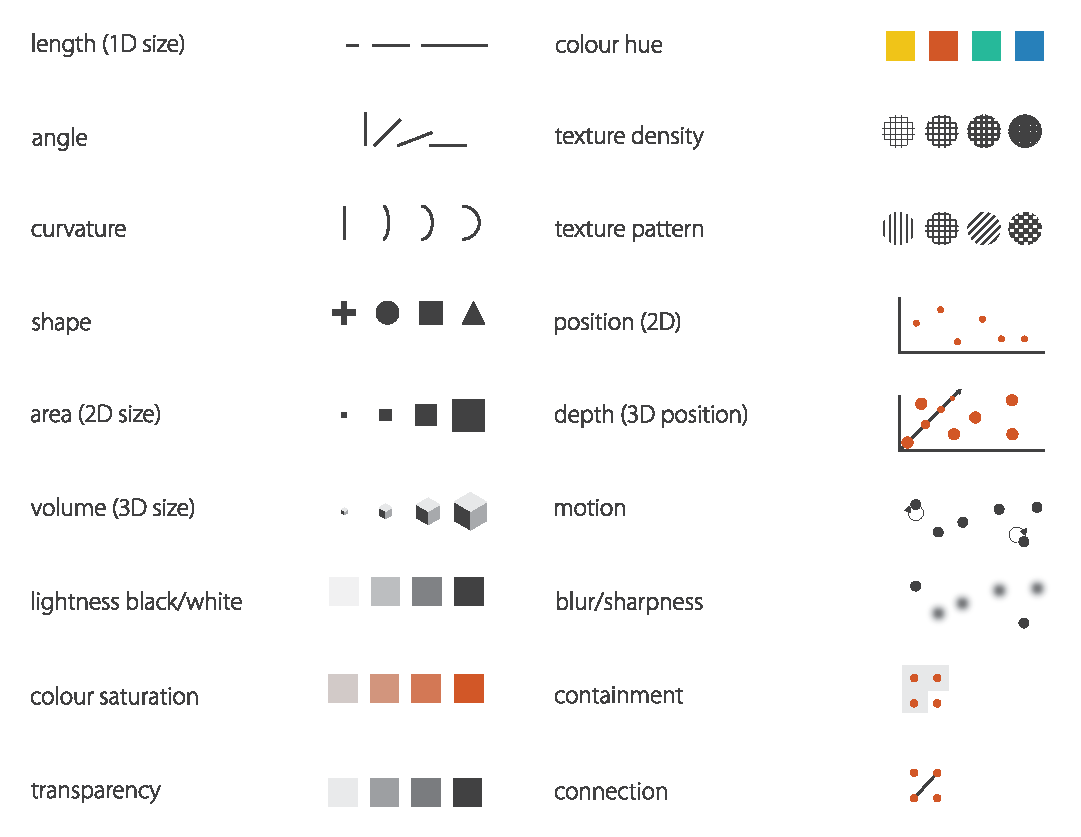
\includegraphics[width=\textwidth]{images/related-work/visual-channels.pdf}
\caption{The types of visual channels available for encoding information from Bertin \cite{Bertin:1983:book} and Ware \cite{ware13}.}
\label{fig:visual-channels}
\end{figure}


\subsection{The Visual Channels and When They Should be Used}
\label{sec:retinal_variables}

This section is organised as follows.
We first introduce the categorisations of visual channels in \ref{sec:viscat}.
This is followed by an investigation of the strengths of visual channels in representing particular types of data in \ref{sec:vispower}.
In \ref{sec:semmapping_vischan} we investigate how semantics can influence the use of particular visual channels.
Finally, in \ref{sec:gestalt}, we introduce Gestalt effects.

\subsubsection{Categorisation of visual channels}
\label{sec:viscat}
Jacques Bertin classified what he termed retinal variables into two categories:
planar (location/position); and 
retinal (size, colour, shape, orientation, texture, and brightness) \cite{Bertin:1983:book,green98}. 
For the sake of consistency, we refer to both retinal and planar variables as \emph{visual channels} throughout this thesis.
Each visual channel has power in representing particular types of data. 
For instance colour could be used to distinguish between male (blue) and female (pink) but it is not as good for representing quantitative data. 
This is also impacted by the cultural association between some colours and more concrete concepts (\eg, blue for male, red for danger, green for go, and so on) \cite{lin2013selecting}. 
Conversely, position can represent quantitative data very well but is not as good as colour for distinguishing between male and female.
The categorisations provided by Bertin were:

\begin{itemize}
\item \emph{associative}: channels facilitating grouping of all elements of a variable despite differing values, \eg, texture, colour, orientation, and shape;
\item \emph{selective}: channels facilitating selection of one category of data, determine the location of visual items with this same category and ignore others, \eg, planar, size, brightness, texture, colour, and orientation variables;
\item \emph{ordered}: channels that facilitate visual ranking of data, \eg, planar, size, brightness, and texture; and
\item \emph{quantitative}: permits extraction of ratios without the need to inspect a legend, \eg, planar and size.
\end{itemize} 

This categorisation is immediately useful since it helps restrict the choice of visual channels depending on the data types that are to be represented. 

\subsubsection{The Power of Visual Channels}
\label{sec:vispower}
What would be more useful are metrics to indicate how the visual channels presented by Bertin are ordered, where the ordering says which visual channels best represent types of information.
So far, metrics are only available to quantify the accuracy of visual channels in representing quantitative data. Stevens \cite{stevens1975} first started measuring the power of variables such as brightness, luminance, length, area, and colour saturation in terms of the stimulus magnitude versus perceived psychological magnitude. 
He found that length was most accurate, with a one-to-one mapping, luminance was perceived greater than intended (1.2), while area and brightness were perceived less than intended (0.7 and 0.5 respectively). 
Performing the worst, colour saturation gave a perceived effect 1.7 times the intended stimulus. 
Stevens found that the majority of stimuli, which included heat, pain, vibration, and duration showed magnified or reduced perceived strength. 
Only length providing one-to-one associations between what the intended stimulus was and how it was perceived. 
A subset of the results from these experiments have been reproduced in Figure \ref{fig:stevens-results}.

\begin{figure}[h!]
\centering
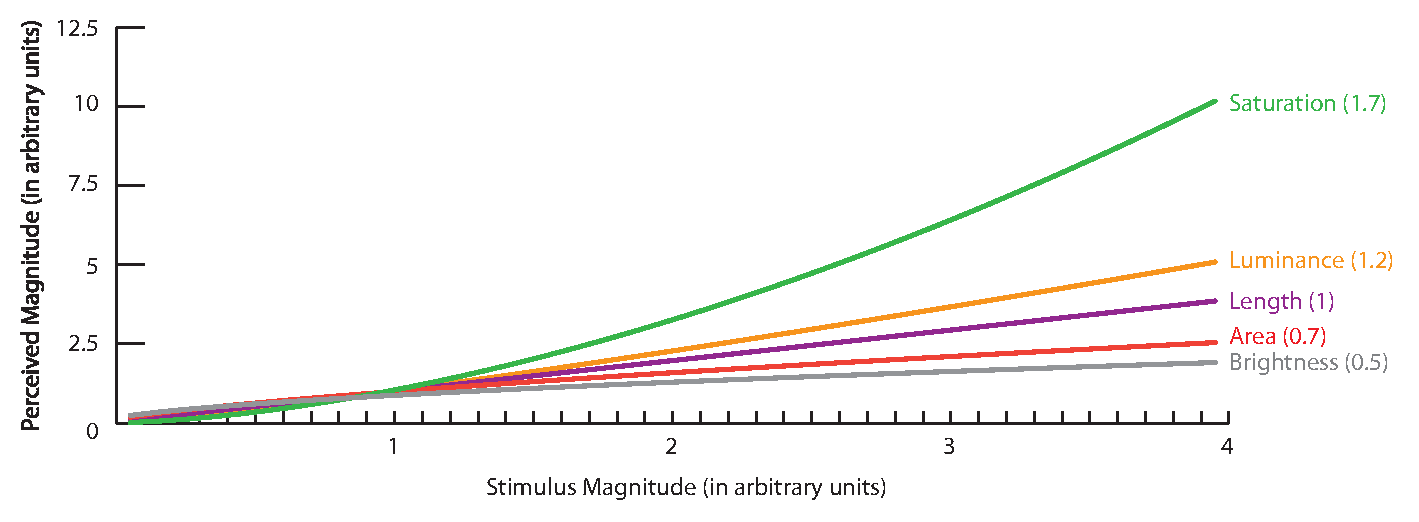
\includegraphics[width=\textwidth]{images/related-work/stevens-psychometrics.pdf}
\caption{A subset of the stimuli and perceived strength versus actual strength by Stevens \cite{stevens1975}.}
\label{fig:stevens-results}
\end{figure}


\begin{figure}[h!]
\centering
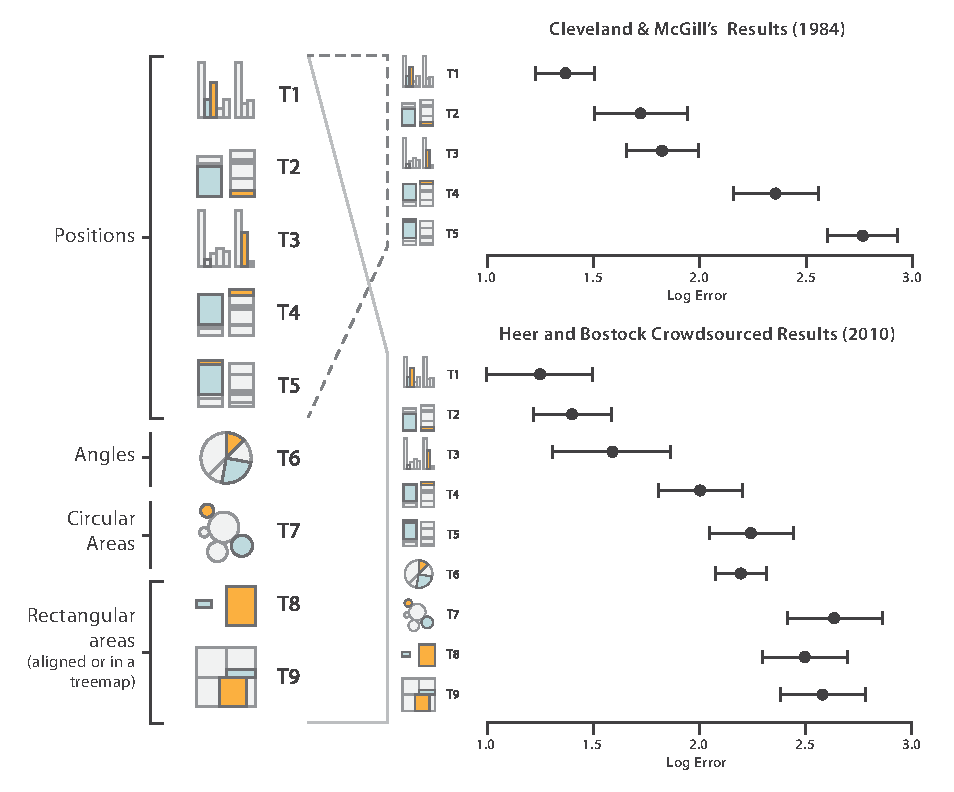
\includegraphics[width=\textwidth]{images/related-work/cleveland_heer_results}
\caption{Observed error rates for different types of visualization using various visual channels to encode the information by Cleveland and McGill \cite{cleveland1984graphical} and Heer and Bostock \cite{heer2010crowdsourcing}. Image adapted from Heer and Bostock \cite{heer2010crowdsourcing}.}
\label{fig:cleveland_heer_results}
\end{figure}

Further to this, research undertaken by Cleveland and McGill \cite{cleveland1984graphical} and recently validated by Heer and Bostock \cite{heer2010crowdsourcing} extended the metrics available for these visual channels as shown in Figure \ref{fig:cleveland_heer_results}. 
This ranking is extrapolated from a series of psychophysics experiments where users are presented with pairwise charts and are asked a series of questions about the underlying data, \emph{e.g.,} what is bigger, A or B. 
The accuracy (and in some cases, response times) for a number of questions are measured. 
For example, in the case of quantitative data, users would be asked what the biggest values are when presented with scatter plots (position), bar charts (length), or bubble charts (area). 
The ``best'' representation is that which obtains the most accurate interpretation from users on average. 

\begin{figure}[h!]
\centering
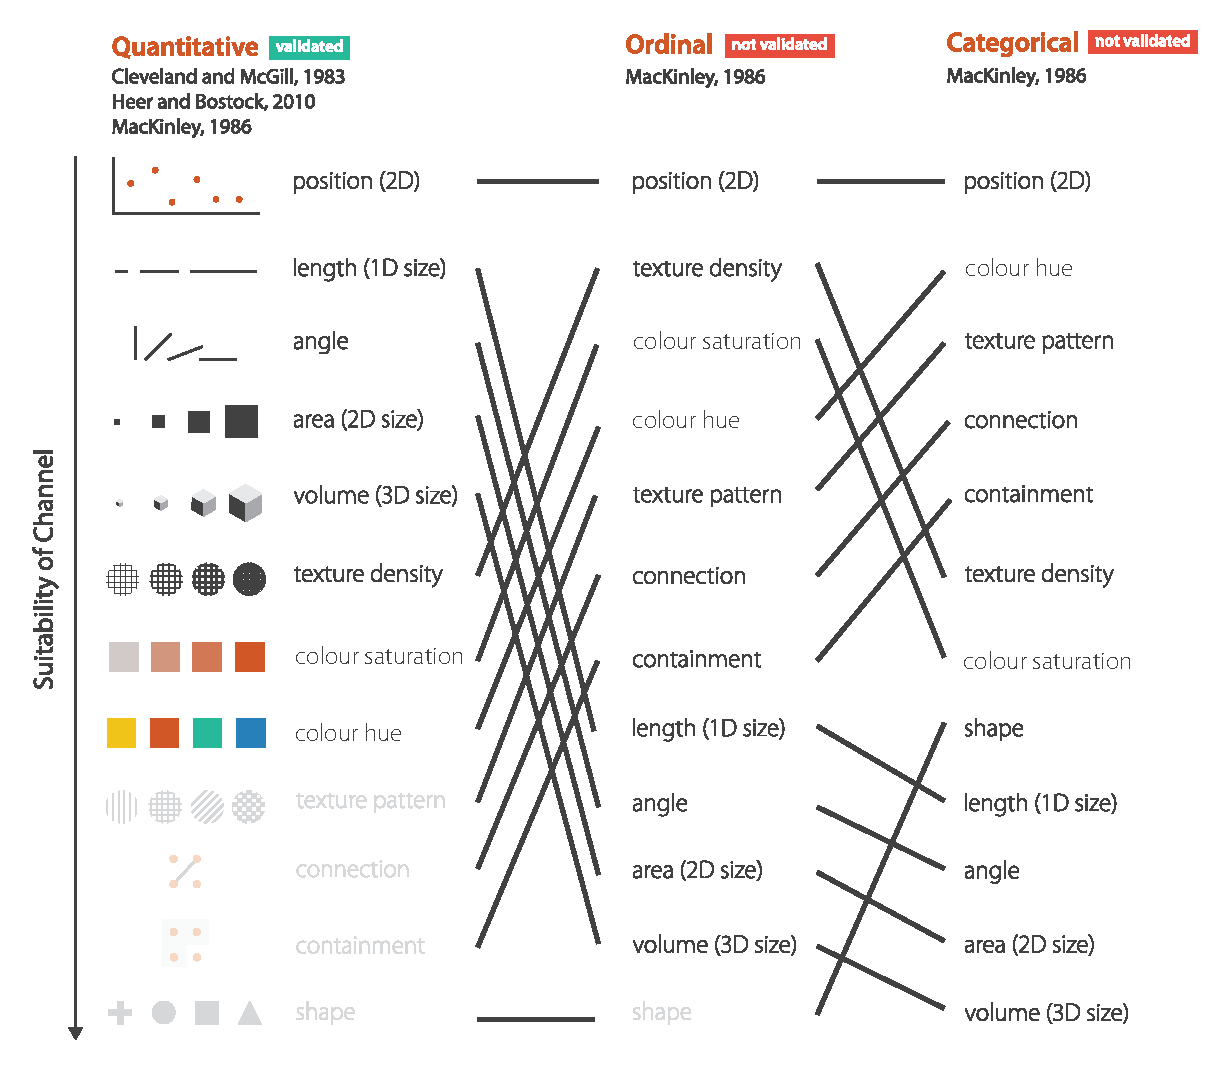
\includegraphics[width=\textwidth]{images/related-work/visual-channel-ordering.pdf}
\caption{A subset of the visual channels from Figure \ref{fig:visual-channels} ordered by MacKinlay\cite{mackinlay1986automating}, Cleveland and McGill \cite{cleveland1984graphical}, and Heer and Bostock \cite{heer2010crowdsourcing}.
Mappings for quantitative visual channels have been validated, however those for ordinal and categorical mappings have not been experimentally validated.
Some visual channels are not applicable to certain data types and these are faded out.}
\label{fig:channel-ordering}
\end{figure}

This ranking was extended to ordinal and categorical data types by MacKinlay \cite{mackinlay1986automating}; however this ranking is not empirically validated, therefore should be taken with a degree of caution. 
Figure \ref{fig:channel-ordering} is derived from \cite{mackinlay1986automating} and serves to represent this ordering, taking note of the fact that ordinal and categorical orderings posed by \cite{mackinlay1986automating} have not been experimentally validated. 

\begin{figure}[h!]
\centering
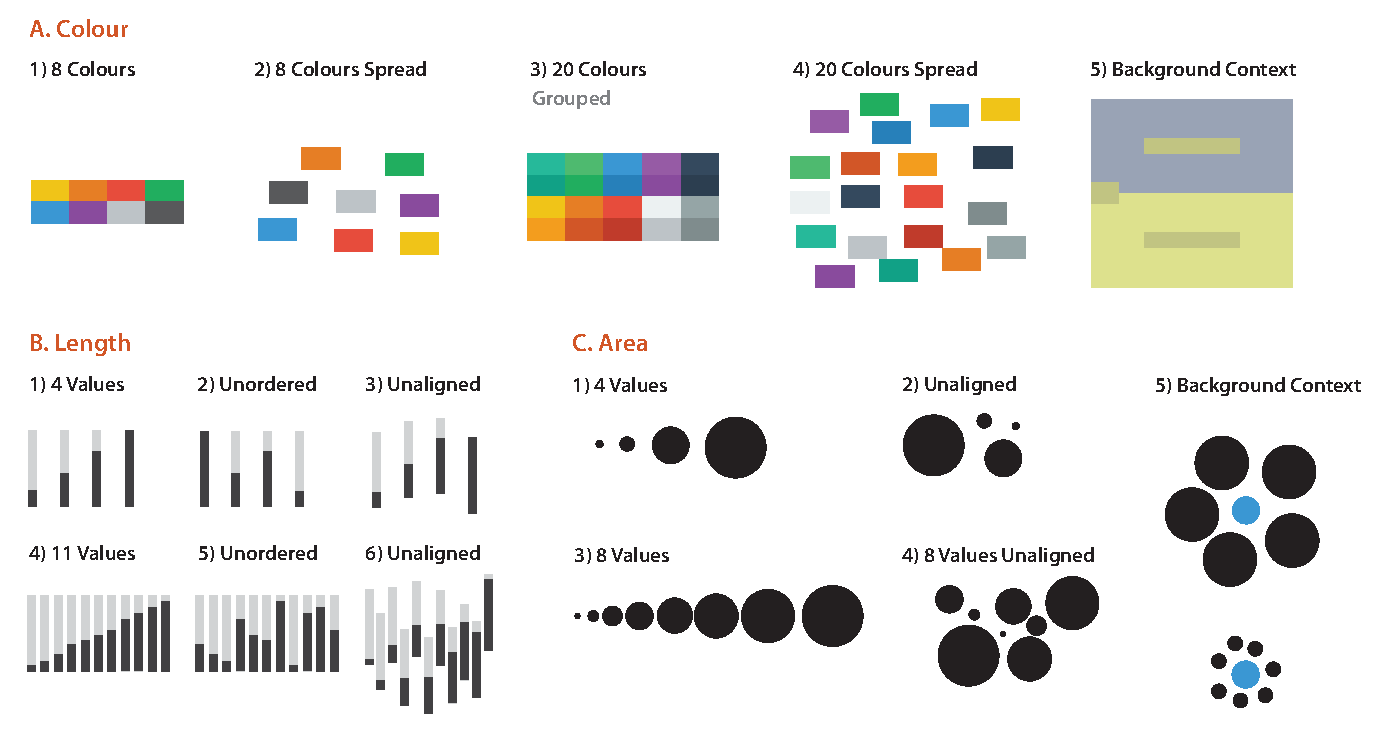
\includegraphics[width=\textwidth]{images/related-work/context-comparison}
\caption{When using various visual channels, we are limited by the number of distinct values we can represent and perceive. Comparison hindered or enabled by the number of values (bins or steps) within each visual channel, their arrangement, and background.}
\label{fig:value-comparison}
\end{figure}

The experiments by MacKinlay and others showed that an accurate interpretation of a value could be made when there exists a sufficiently large distance between the visual elements being compared \cite{mackinlay1986automating, cleveland1984graphical, heer2010crowdsourcing}. 
There are a number of factors that influence comparison:
1) the number of values in the comparison space;
2) the Euclidean distance between those values;
3) the spatial arrangement of the values; and
4) background interference.

Figure \ref{fig:value-comparison} serves to illustrate the contributions these four factors make when comparing different colour hues, lengths, and areas. \\

\noindent\textbf{Colour hues}. It is widely regarded in the visualization community that a visualization should have no more than twelve colours to represent categorical information. 
Having more would make it difficult for the user to distinguish between steps or variations within the limited number of hues available.
Hitt suggested that between no more than five and seven colours should be in a visual display \cite{hitt1992retrofit}. 
Healey validated this statement in an experiment \cite{healey1996choosing}.
Ware proposed a mechanism that divided the hues in to families yielding around eight to twelve distinguishable colours, although this is not experimentally validated \cite{ware13}.
Haroz and Whitney showed how an increase in the number of colours increased response times when finding a target of interest (avoidable through colour grouping\cite{haroz2012capacity}).  

This limitation is illustrated in Figures \ref{fig:value-comparison} A1 and A3 which show two colour maps, one with eight categories, the other with twenty. 
The increased number of categories in Figure \ref{fig:value-comparison} A3 reduces the ``distance'' between the colours. 
Due to the limited number of hues, and the limited number of steps within those hues \cite{ware13}, it becomes more difficult to detect the differences between colours.  
This problem becomes more evident when the grouping of colours is removed in Figure \ref{fig:value-comparison} A4 where some of the greens, oranges, purples, dark blues, and greys look very similar. 
When a user is now asked to perform a visual search task for a hue of orange, he (or she) will find it more difficult to find the orange value amongst the several variations of orange, than one single value of it. 
In addition, colour comparison becomes more difficult when background colour is taken into consideration. 
Due to how the visual system works, and in particular lateral inhibition (which will be discussed later in this chapter), the visual system is continually trying to improve contrast to facilitate edge detection. 
This influences how colours are perceived relative to the background since the brain will dull down one area of an image to make another stand out. 
This causes the classic optical illusion shown in Figure \ref{fig:value-comparison} A5.\\

\noindent\textbf{Length}. Figures \ref{fig:value-comparison} B1 and B4 show how the number of values decreases the perceptual distance between each bar.
The effect is shown with four values which can be perceived well regardless of whether they are sorted or not.
Increasing the number of values results in more data needing to be represented in the same display space.
When sorted, as in Figure \ref{fig:value-comparison} B4, comparing bars is simple.
When unordered in Figure \ref{fig:value-comparison} B5, it is now harder to compare bar height \cite{Chung29112013}. 
When unaligned in Figure \ref{fig:value-comparison} B6, it is very difficult. \\ 

\noindent\textbf{Area}. Figures \ref{fig:value-comparison} C1 and C3 again show how the number of values decreases the distance between visual items. 
When aligned and ordered, comparison is again relatively straightforward, however when unaligned and unordered, the areas in 
Figure \ref{fig:value-comparison} C4 become difficult to compare with numerous areas appearing to be the same size.
Finally, Figure \ref{fig:value-comparison} C5 shows how the background can influence perception of size with two blue circles of the same area appearing to be different due to the size of the surrounding circles.

Consider that in Figure \ref{fig:value-comparison} C5 those blue circles represented the same number of admissions to hospitals in different areas, the bottom blue circle will appear bigger as a result of the surround. 
If other areas have lower admissions, the size of the inner circle will look bigger.
How might that affect policy making, or public perception if shown in a newspaper or TV broadcast where users could not interrogate the visualization for details?

Ensuring there is sufficient visual difference between areas, especially when the task demands accurate comparisons, is imperative to the creation of an effective visualization. 


\subsubsection{Semantic Mapping of Visual Channels}
\label{sec:semmapping_vischan}
Ware \cite{ware2010visual} presents the concept of `semantic mappings' where ``graphical codes''/patterns are inherently related to how humans perceive information in everyday life.
For example, larger objects represent bigger quantities or products closer together in a supermarket are likely to be more similar to each other than objects further away \cite{ware2010visual}. 
In natural language, to reinforce ideas and to help humans build an understanding of hows things are related or positioned, the phrases ``connected to'', ``built on'' or ``contained within'' are used to provide spatial analogies \cite{ware2010visual}. 
In the same way these phrases are used to aid understanding in text, equivalent visual patterns can be used to represent such concepts in visualizations. 
These patterns or ``graphical codes'' are presented by Ware \cite{ware2010visual} and reproduced in Figure \ref{fig:semantic-mappings-ware}. 

\begin{figure}[h!]
\centering
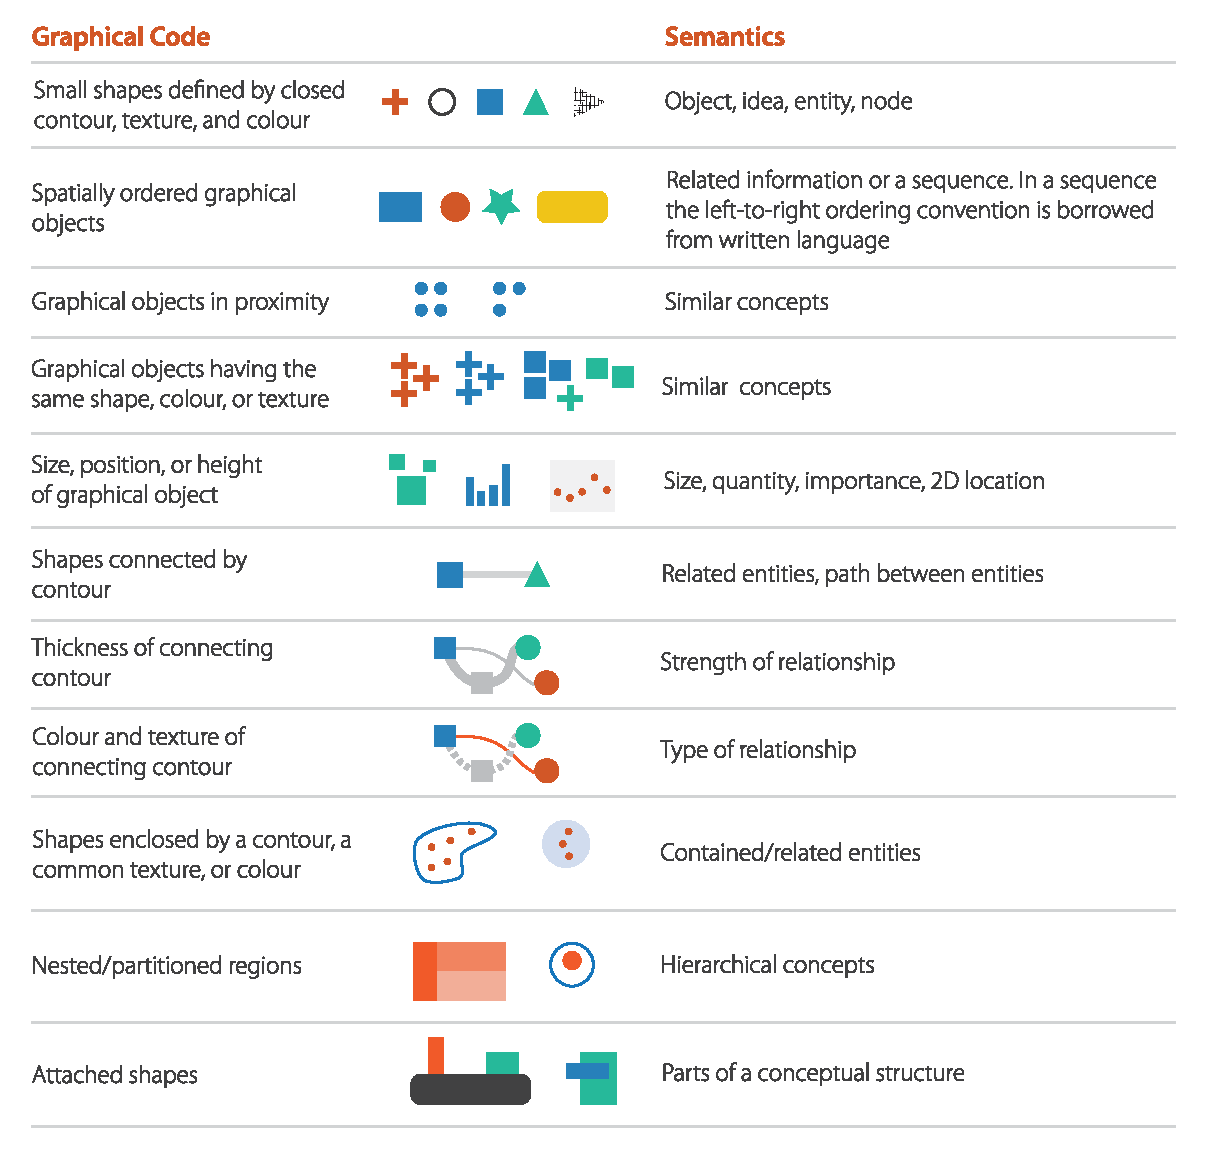
\includegraphics[width=\textwidth]{images/related-work/semantic-patterns.pdf}
\caption{Graphical codes and their semantic mapping. Adapted from \cite{ware2010visual}.}
\label{fig:semantic-mappings-ware}
\end{figure}


\subsubsection{Gestalt Laws}
\label{sec:gestalt}
\begin{chapquote}{Kurt Koffka}{``The whole is other than the sum of the parts.''}
\end{chapquote}


\begin{figure}[h!]
\centering
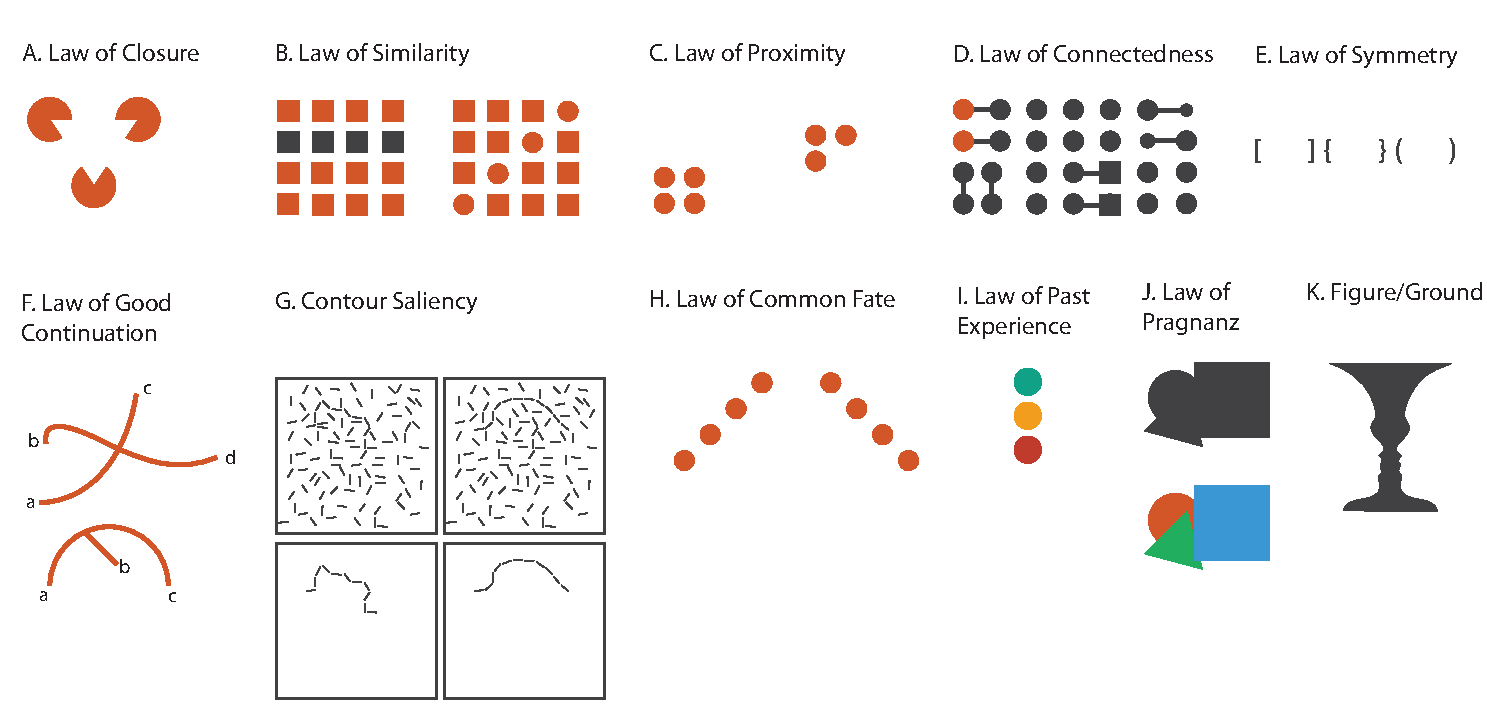
\includegraphics[width=\textwidth]{images/related-work/gestalt.pdf}
\caption{A) \emph{Law of closure} - we look for a single pattern amongst an arrangement of more complex elements. This example shows the Kanisza triangle \cite{ginsburg1975illusory}. 
B) \emph{Law of similarity} - elements with common features are perceived more similar than those that do not have those features. 
C) \emph{Law of proximity} - elements that are closer to each other are perceived more similar. 
D) \emph{Law of connectedness} - connected elements are perceived more related with a stronger effect than colour, shape, size, and proximity. 
E) \emph{Law of symmetry} - we see three groups instead of six individual items. Additionally, the strength of symmetry is greater than proximity. 
F) \emph{Law of good continuation} -  lines are linked when collinear - \textbf{a} and \textbf{c} and \textbf{b} and \textbf{d} in the top example appear as one as does \textbf{a} and \textbf{c} in the bottom image. However \textbf{a} and \textbf{b} do not appear to belong to the same line (adapted from \cite{kandel2012principles}). 
G) \emph{Contour saliency} - smooth contours can be perceived more easily than a jagged contour (adapted from \cite{kandel2012principles}). 
H) \emph{Law of common fate} - groups of items going towards a particular direction are perceived as one. Here, two groups can be perceived. 
I) \emph{Law of past experience} - our experiences have an impact on how we perceive often abstract items. In this example, with three ellipses coloured green, amber and red, we perceive a traffic light although the intention of the designer may have been different. This is a common factor with colour where different colours in different countries mean different things. 
J) \emph{Law of Pragnanz} - this refers to the brain's preference to split complex objects in its simplest constituent parts.
K) \emph{Figure/Ground} - the visual system processes parts of the image as the main object of interest (figure) and the rest as the background (ground).}

\label{fig:gestalt}
\end{figure}

Many of these graphical codes are derived from \emph{Gestalt} psychology, translated from German to mean ``configuration or form'' \cite{kandel2012principles}. 
\emph{Gestalt} psychologists posed the theory that a visual system processes sensory information about the colour, distance, form, and motion of objects through the application of a set of rules. 
This theory gave rise to a number of ``Gestalt laws'', specifying how certain configurations of objects, \eg, proximity, similarity, good continuation, closure, connectedness, common fate, familiarity, and symmetry play into our perception of the world around us. 
These laws are illustrated in Figure \ref{fig:gestalt} and are formed through the observation of four key points:

\begin{itemize}
\item \textbf{Emergence} - the whole object is identified ahead of its constituent parts; that is, we will look at the outline of an object and match these outlines to what we already know then identify the rest of the smaller parts.
This refers to global-local processing and is discussed more in Section \ref{sec:global_local_processing};
\item \textbf{Reification} - our ability to fill in the gaps as in Figure \ref{fig:gestalt} A;
\item \textbf{Multi-stability} - is illustrated in the figure/ground example in Figure \ref{fig:gestalt} K which shows the stable/unstable depiction of what is figure and what is ground. 
We can see the two faces or a vase depending on whether or not you see the black as the figure or ground. 
The ability to go between the vase and the two faces makes the relationship unstable; and
\item \textbf{Invariance} - the innate ability of our visual systems to identify items with a tolerance for change allows our visual system to recognise a square even if its rotated or slightly distorted or a face even if viewing a profile and not the frontal view.
\end{itemize}


\section{The Visual System}
\label{sec:vis-processing}

\begin{chapquote}{Richard L. Gregory, Eye and Brain, 1966}{``We are so familiar with seeing, that it takes a leap of imaginations to realise that there are problems to be solved. But consider it. We are given tiny distorted upside-down images in the eyes and we see separate solid objects in surrounding space. From the patterns of stimulation on the retina we perceive the world of objects and this is nothing short of a miracle.''}
\end{chapquote}

\emph{``How do we see?''} has been a question behind a large body of research for many decades and scientists are still trying to answer it. 
There is no complete model describing the complete visual system in terms of how we go from vision to understanding.
However, there is a great deal of validated research into the building blocks of visualization and how various visual channels introduced earlier are processed by our visual system.
This research is based largely on experiments performed on animals (\eg, cats by Hubel and Wiesel in 1958 \cite{hubel1959receptive}), and later in primates, whose visual system is largely homologous with that of humans. 

This section presents an overview of the basic principles of visual processing, with a focus on details relevant for visualization design.
Acting as a primer for discussions around pre-attentive processing, channel separability, and visual hierarchy, this section presents an overview of the basic principles of visual processing.
This encompasses research on how the visual system is physically arranged, how a visual scene is decomposed into its constituent parts (local areas of contrast), then recomposed by the visual system.

Three coordinated and cross-interacting processes detailed below are imperative to the visual system, extending from the eyes through to the visual cortex at the rear of the brain:  
\begin{itemize}
\item \textbf{Low-level processing} - at this level of processing, visual primitives, those being colour, local contrast, orientation, binocular disparity (different images of the same scene from each eye) for 3D depth perception, and movement are processed \cite{kandel2012principles}.
This will be described below in more detail and relies on cells in the retina, the lateral geniculate nucleus, and the primary visual cortex (V1) and V2 at the rear of the brain;
\item \textbf{Intermediate-level processing} - here, the scene is analysed given the visual primitives obtained at the previous level of processing to perform contour integration, identify object boundaries, analyse surface properties, depth and segmentation, determine object motion, and what is the figure versus the ground \cite{kandel2012principles}.
\item \textbf{High-level processing} - in the \emph{ventral stream} (what pathway) for object identification based on contours, surfaces, movement, and depth found in the visual processing stages in combination with past experience; and the \emph{dorsal stream} (where pathway) for motion detection and guidance of movement in the 3D world.
\end{itemize}

\subsection{Low-level Processing}
Low-level processing starts in the retina. 
When we process a visual scene, the rods (achromatic sensitivity) and cones (chromatic sensitivity) become activated by light photons with the result being the inhibition of release of a neurotransmitter called glutamate which normally moves across a synapse onto what are called bipolar cells. 
Cones are linked to two types of bipolar cells (ON/OFF) whereas rods have only one type of bipolar cell. 
ON bipolar cells are inhibited (hyperpolarised) by the presence of glutamate and OFF bipolar cells are excited (depolarised) by glutamate. 
When glutamate stops being released from the photoreceptor, the ON bipolar cell becomes more depolarised and the OFF bipolar cell less depolarised. 

Rods synapse with a special type of bipolar cell that interact with cells named amacrine cells (not ganglion cells as is the case for cones). 
These amacrine cells create a horizontal connection which enables lateral inhibition of the bipolar cells connected to cones. 
The horizontal connections help in creating visual acuity through inhibition of the less illuminated areas of a receptive field, where 
less well-illuminated areas have their signal reduced leaving the more-enhanced illuminated areas. 
This results in better contrast between the better and less well-illuminated areas in the visual field. 

There are many more photoreceptors in the retina than there are axons (~1\% of total receptors) in the optic nerve to represent them \cite{kandel2012principles}. 
Therefore, the first levels of visual processing occur directly in the retina through comparison and aggregation of photoreceptor outputs. 
At this point in the visual system, this comparison and aggregation occurs to help in detecting local contrast (for edge detection). 
To achieve this, one retinal ganglion cell compares and summates the responses of a varying number photoreceptors, with the number of photoreceptors directly related to the proximity of the photoreceptors to the fovea. 
This relationship between a retinal ganglion cell and the photoreceptors associated with it is termed the \emph{receptive field of the ganglion cell}. 
The receptive fields can be categorised into two main types, \emph{on-centre} and \emph{off-centre} which are illustrated in Figure \ref{fig:receptive-fields}. 
These fields allow for detection of contrast since they are selective for differences in illumination, and therefore contours/edges in the image \cite{kandel2012principles}. 
A smaller receptive field near the fovea allows for discrimination of fine detail (high spatial frequencies) and larger receptive fields towards the periphery are tuned for more coarse details (low spatial frequencies). 
Additionally, motion is shown to elicit a stronger response in the ganglion cells than a non-moving object \cite{kandel2012principles}. 

\begin{figure}[t!]
\centering
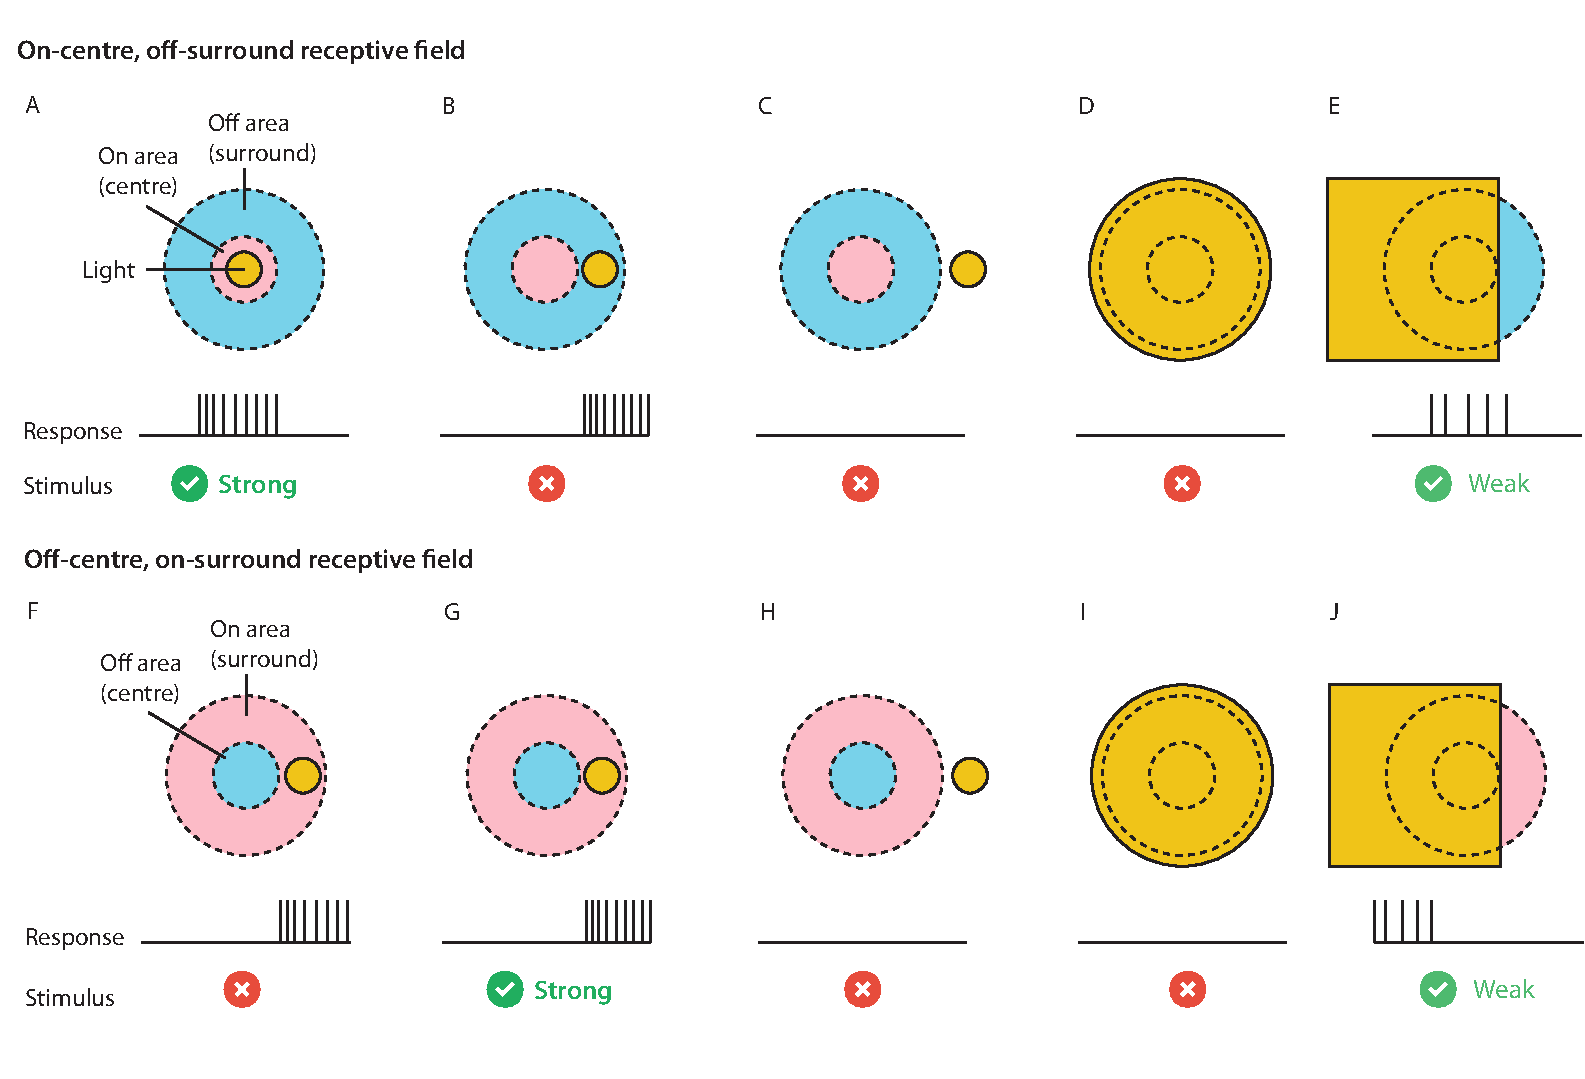
\includegraphics[width=\textwidth]{images/related-work/receptive-field}
\caption{Two types (\emph{on centre and off centre}) of receptive fields stimulated under five conditions. 
A) The response of the ganglion cell's receptive field is strongest when the light is shown directly in the centre. 
The response would be the opposite for an \emph{off-centre, on-surround} receptive field as shown in F. 
B) Light shone on the surround area causes a response in the receptors, however there is no stimulus recorded due to the selectivity of the cell. This is the opposite in the \emph{off-centre, on-surround} as shown in G. 
C) and H) Light outside the receptive field obviously records no stimulus in both types of receptive field. 
D) and I) When light covers the whole field, there is no response recorded at all - this shows how this type of cell is selective for contrast. 
E) and J) Weak responses are generate when the receptive field is partially covered by light.} 
\label{fig:receptive-fields}
\end{figure}

\begin{figure}[h!]
\centering
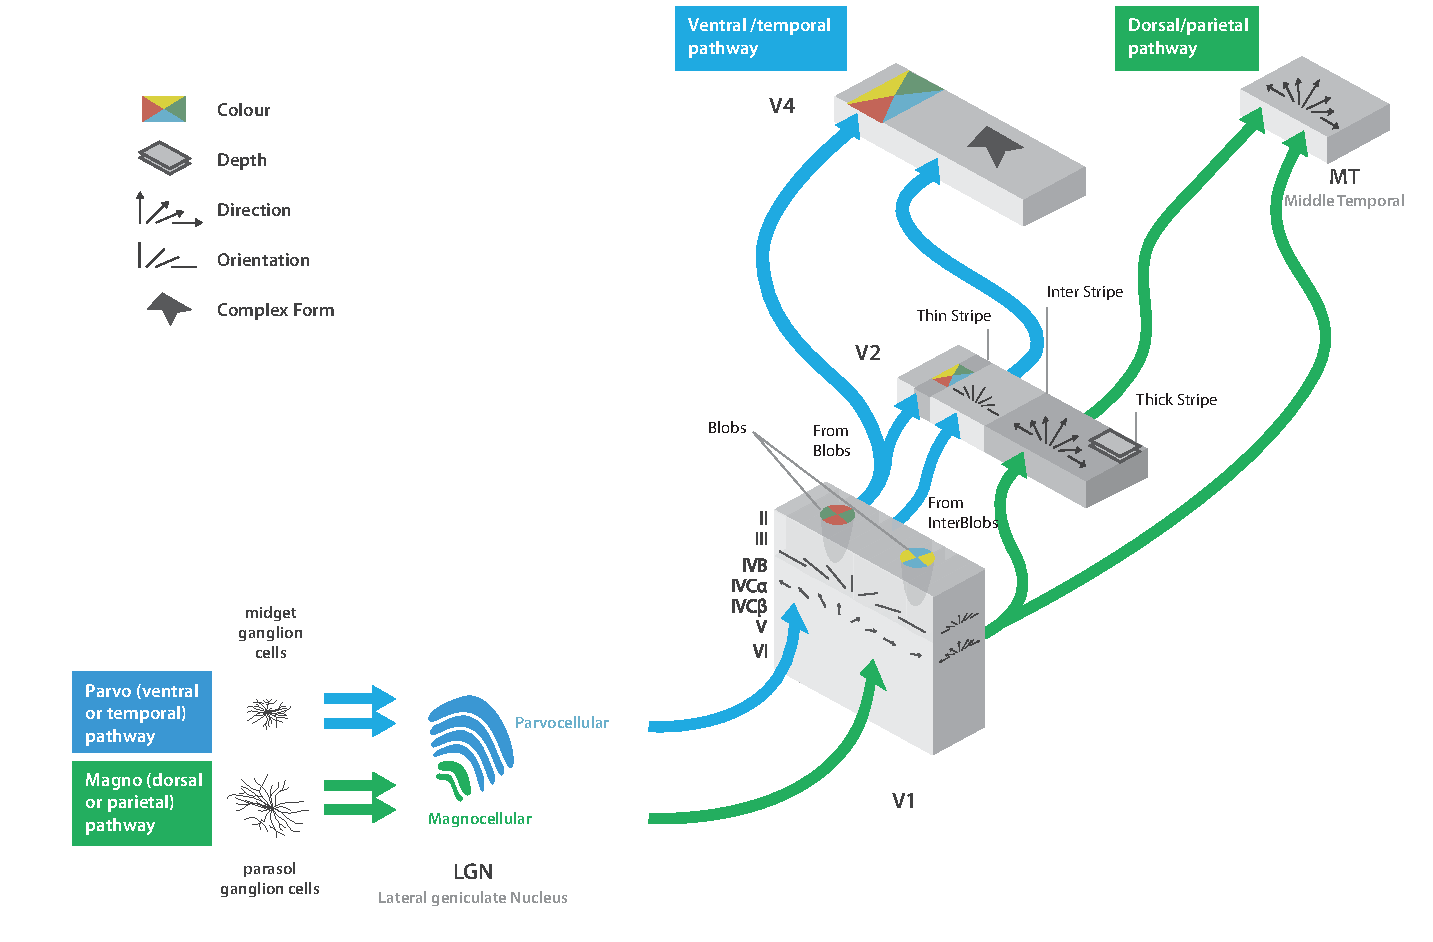
\includegraphics[width=\textwidth]{images/related-work/parallel-processing-visual-pathways}
\caption{Parallel processing in visual pathways adapted from Kandel \etal, 2012 \cite{kandel2012principles}. 
Object identification is conducted in the ventral stream through cells selective for form and colour information. 
Visually-guided movement is performed in the dorsal stream with use of movement sensitive cells. 
There is significant interconnectivity between these two pathways.}
\label{fig:visual-processing}
\end{figure}


Retinal ganglion cells exist in three main forms in primates, as M (magno)-, P (parvo)-, and K (koniocellular)-ganglion cells.
M and P ganglion cells are spatio-temporal filters that feed into two parallel pathways in the visual system (magno and parvo) \cite{merigan1993parallel}.
M cells do not select for colour, but have a greater sensitivity to rapidly moving stimuli \cite{merigan1993parallel}.
P cells have greater spatial resolution, selectivity for colour, and the ability to respond to slowly changing or slowly moving stimuli \cite{merigan1993parallel}.
K cells are interspersed between M and P ganglion cells and are said to be involved in relaying colour information and low resolution details to V1 \cite{hendry2000koniocellular}.
Figure \ref{fig:visual-processing} shows a simplified view of how input comes from the LGN in to the visual cortex via a parallel stream with object recognition facilitated by the parvo pathway, and visually guided movement facilitated by the magno pathway.
Communication occurs along these pathways via signals aided by the firing of neurons (action potentials).
These signals pass along the optic nerve, through the optic chasm, down the optic tract, into the lateral geniculate nucleus (LGN) which also contains contrast processing cells, to the optic radiation, and finally into the visual cortex.
This model is often used to illustrate the visual system, however there is evidence to suggest that the magno and parvo pathways have significant flow of information between them \cite{merigan1993parallel}.
Location information is preserved from the retina in what is called a retinotopic map, a direct mapping between an area in the retina and its respective processing area in the LGN and visual cortex.

Moving from the LGN to the visual cortex there is a change in the structure of the receptive fields which represents a shift in the type of visual processing occurring within the visual system.  

The primary visual cortex is presented as a columnar arrangement of neurons sensitive to orientation \cite{hubel1959receptive}, direction, and colour-sensitive neurons (blobs with small circular receptive fields) \cite{horwitz2012nonlinear} interspersed regularly across the structure (Figure \ref{fig:visual-processing}). 
This columnar structure features right and left eye dominant columns that alternate every 750-1000$\mu$m alongside criss-crossed columns selective for particular orientations \cite{horton1984mapping}. 
Orientation-selective neurons are split into two types: simple; and complex. 
Simple neurons have ON and OFF subregions where if there a bar of light of a particular orientation enters the ON region, the neuron fires. 
The neuron also fires when the bar leaves the OFF region. 
Complex neurons on the other hand fire continuously as the bar moves across its receptive field. 
These neurons were first discovered by Hubel and Wiesel in 1958 in experiments performed on the cat \cite{hubel1959receptive} and are illustrated in Figure \ref{fig:orientation-cells}. 
They are thought to be arranged into what are termed \emph{hyper-columns} representing the populations of neural cells selecting for specific orientations in the full 180$^{\circ}$ of possibilities. 
These hyper-columns are thought to repeat across the visual cortex every 750$\mu$m.

\begin{figure}[t!]
\centering
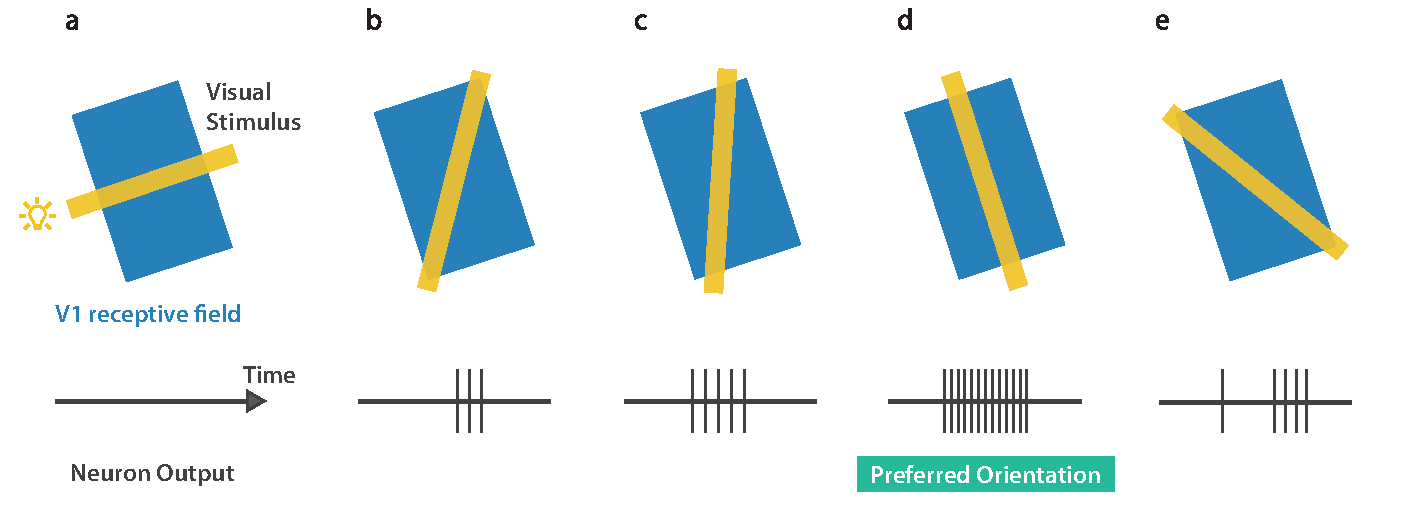
\includegraphics[width=\textwidth]{images/related-work/orientation.pdf}
\caption{A receptive field (blue) and the neural response to a flashing light bar stimulus (yellow). 
The examples show how specific neurons have distinct preferences for orientation with a) performing worst and d) providing the strongest response. 
Adapted from \url{http://neuroscience.uth.tmc.edu/s2/chapter15.html}.}
\label{fig:orientation-cells}
\end{figure}

As illustrated in Figure \ref{fig:orientation-cells}, these neurons will fire whenever presented with a stimulus, in this case a bar of light with a particular orientation. 
This means that for every position in the retinotopic map, if there is contrast, these positions will be converted into local contours.
These local contours are thought to be the basis of shape and surface detection in the intermediate-level processing stage which will be detailed further below.\\

\subsection{Intermediate-level processing}
Intermediate-level processing involves convergence of the many line segments and surface properties detected in low-level processing and the construction of complex patterns and objects. 
This process is thought to involve: contour integration; identification of object boundaries and therefore identification of the figure versus ground; object motion; and analysis of surface properties, depth, and segmentation. 
A key property of the cells involved at these stages of visual processing is the widening receptive field to capture overall details of many smaller parts (\eg, local contours or local regions of surface change).

\subsubsection{Contour Integration}
As illustrated in Figure \ref{fig:gestalt} G, Gestalt laws state that smooth contours are more salient (they ``pop-out'') when compared to more jagged contours.
This may be explained by horizontal connections that exist between columns with similar orientation preferences in area V1 of the visual cortex \cite{kapadia1995improvement}. 
Therefore when a straight line is observed in one column, a preference is enforced via horizontal connections for columns with a similar orientation \cite{kapadia1995improvement}.
This mechanism could enforce a preference for continuity (smooth lines). 

Next, there is \textbf{identification of object boundaries} also referred to as figure/ground discrimination \cite{lee2003computations, qiu2005figure} or border ownership (BOWN) which is said to occur largely in V2. 
We see a three-dimensional (3D) world even though our eyes capture a two-dimensional (2D) scene. 
To be able to infer depth as the third dimension we must look at many visual cues such as shadows, occlusion, differences between both eyes (binocular disparity), and previous knowledge to determine how the three dimensional world is arranged. 
So how does one object relate to another? Is an object the figure or is it the ground? 

There are two competing theories of how the visual system computes this. 
The first is by Lamme \cite{lamme1995neurophysiology} who was the first to find that some neurons fired more frequently to objects in a figure region as opposed to objects in the ground region. 
He proposed that regions in a scene are labeled (region labelling), with closer (occluding) regions labeled the figure, and the further away (occluded) region labeled as the ground.

The second theory by Zhou \etal \cite{zhou2000coding} proposed a more complex model where different regions can be labeled with relative depth orderings followed by border ownership processing. 
The more plausible theory is that put forward by Zhou \etal \cite{zhou2000coding} due to its power in explaining complex figure/ground scenarios such as the previously-mentioned Rubin's vase/faces illusion. 

Qiu \etal \cite{qiu2005figure} built on the work by Zhou \etal \cite{zhou2000coding} to show that area V2 in the macaque monkey employed two computational strategies for establishing the figure from ground. 
One strategy determines local depth order through exploiting binocular stereoscopic information \cite{qiu2005figure}. 
The other exploits Gestalt factors such as closure available through processing the global arrangement of contours\cite{qiu2005figure}. 
Figure \ref{fig:bown} shows a number of examples of the border ownership problem where in Figure \ref{fig:bown} C the figure is considered to be the orange ellipse but when the perspective is changed, the blue shape becomes the figure. 
In each case, ownership of the border is assigned to different objects reflecting their position in 3D space. 
Figure \ref{fig:bown} also depicts what are interactions between BOWN cells using green dotted lines. 
This messaging system is said to excite BOWN cells that are in agreement and inhibit BOWN cells in disagreement to create a depth map with all possible combinations. 

\begin{figure}[t!]
\centering
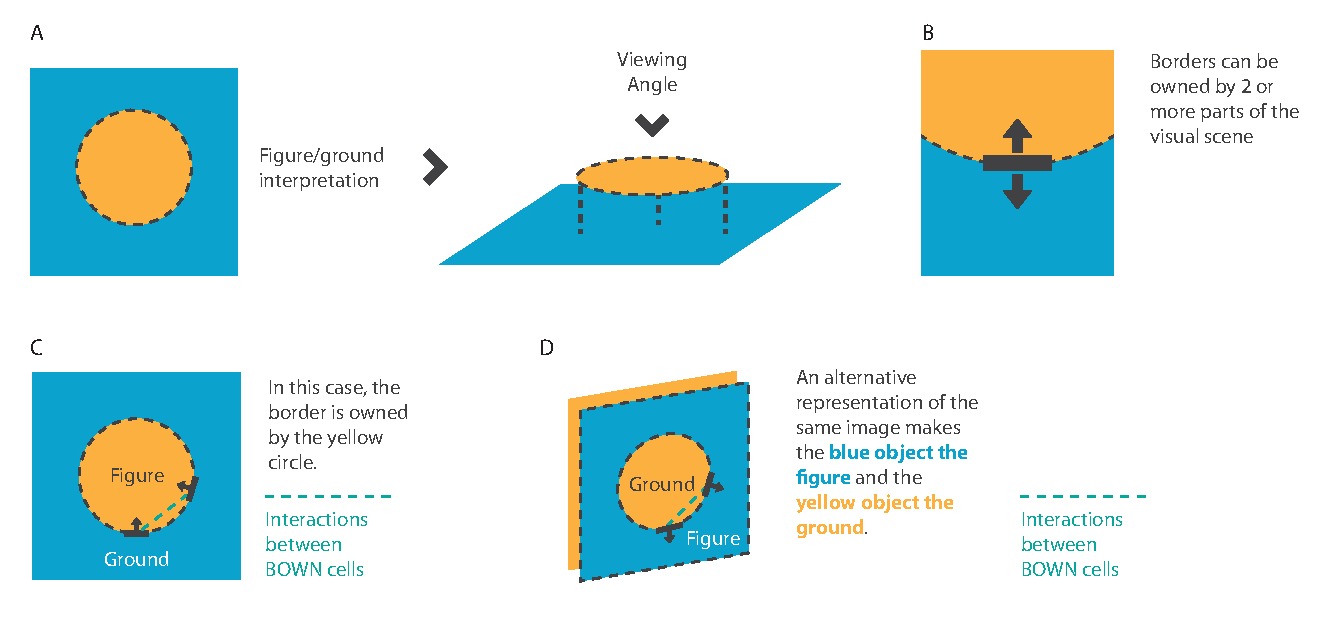
\includegraphics[width=\textwidth]{images/related-work/border-ownership}
\caption{A) This image is interpreted as an orange ellipse on top of a square.
B) A border can belong to two competing regions.
C) A competing side on a boundary becomes the owner which provides the relationship that the circle is the figure, and the rectangle is the ground.
D) An alternative representation of the same image shown in A) shows how depth can change the interpretation of the image.
Green lines illustrate Interactions between BOWN cells which are said to assist with creation of depth maps.}
\label{fig:bown}
\end{figure}

Border ownership appears to be facilitated by three types of neurons identified in V2 \cite{zhou2000coding, qiu2005figure} selective for \emph{side-of-figure} (35\%), \emph{depth order} (40\%) and both \emph{side-of-figure} and \emph{depth order} (21\%) \cite{qiu2005figure}. 
Neurons selective for side-of-figure have a preference for ownership at a particular side as shown in Figures \ref{fig:bown-examples} A and B. 
Figure \ref{fig:bown-examples} A shows how the BOWN neurons respond to a boundary only when it is part of a surface that lies on the preferred side of the cell's receptive field. 
In this case, the neuron is receptive to arrangements where the figure is on the right side. 
This is exemplified further in Figure \ref{fig:bown-examples} B with examples I)1 and II)1 where the spike rate of II)2 is ~4x that of I)1 when the figure is to the right of the receptive field. 
A similar result can be seen in the rest of the examples.  

\begin{figure}[t!]
\centering
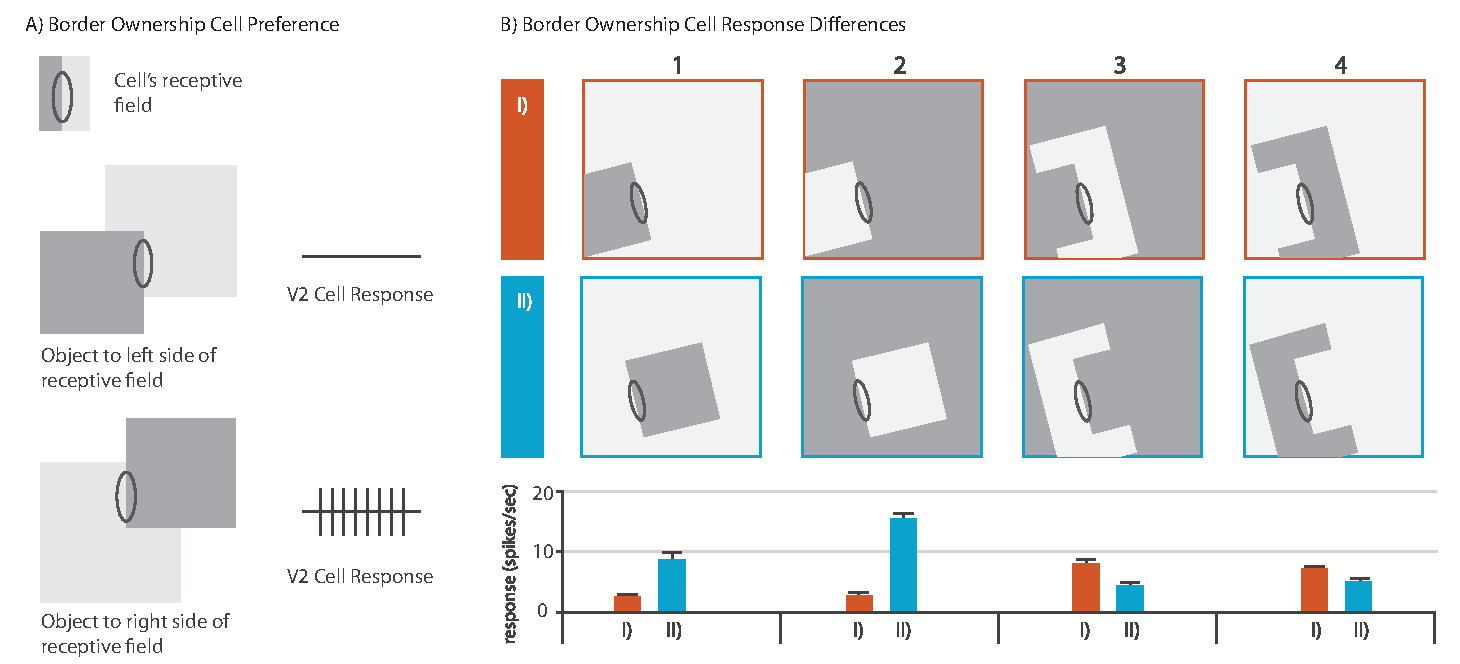
\includegraphics[width=\textwidth]{images/related-work/bown-neurons}
\caption{BOWN sensitive neurons with a preference for right-side figure in the macaque visual cortex. A) V2 cell response when object is on preferred side of a cell's receptive field (in this case, right). B) The oval with the black outline represents the receptive field which remains constant throughout all examples. Examples \textbf{I)} 1 and 2 on the top row (orange) show a number of examples of figure/ground scenarios with border ownership on the left side of the receptive field. The converse arrangement of \textbf{I)} 1 and 2 is shown on the bottom row (\textbf{II} 1 and 2). Examples \textbf{I} 3 and 4 show border ownership on the right side with left side ownership shown in \textbf{II} 3 and 4. Average neural responses are shown for each scenario (\textbf{I)} and \textbf{II)}). Modified from \cite{zhou2000coding, kandel2012principles}.}
\label{fig:bown-examples}
\end{figure}

Through point-wise border ownership calculations across all local contours of an object, with pairwise excitation of agreeing BOWN cells and inhibition of disagreeing BOWN cells, the visual system is able to discriminate between figure and ground and create depth maps.

\subsubsection{Motion Perception}
Analysis of motion is prevalent throughout the visual cortex from the retina \cite{kimspace2014, kandel2012principles} whose cells react as much to movement as to light (a static image would fade from view if it were not for the continuous movements of the eye, called \emph{saccades}) right through to the visual cortex. 
At different levels of the visual processing system, motion information is processed via direction-selective neurons. 
In fact, there are cells in the retina that only respond on the observation of local contours moving in particular directions. This has been shown in rabbits by Barlow \etal \cite{Barlow01021963} and more recently by Kim \etal \cite{kimspace2014}.
Kim \etal showed that such direction-specificity of neurons was present in the retina of mice through ``starburst neurons'' that operated via the process illustrated in Figure \ref{fig:motion-neurons}.
Such direction-specificity is made possible through time-delayed bipolar cells that must be activated in the correct sequence to illicit a response from the neuron \cite{kimspace2014}.

\begin{figure}[t!]
\centering
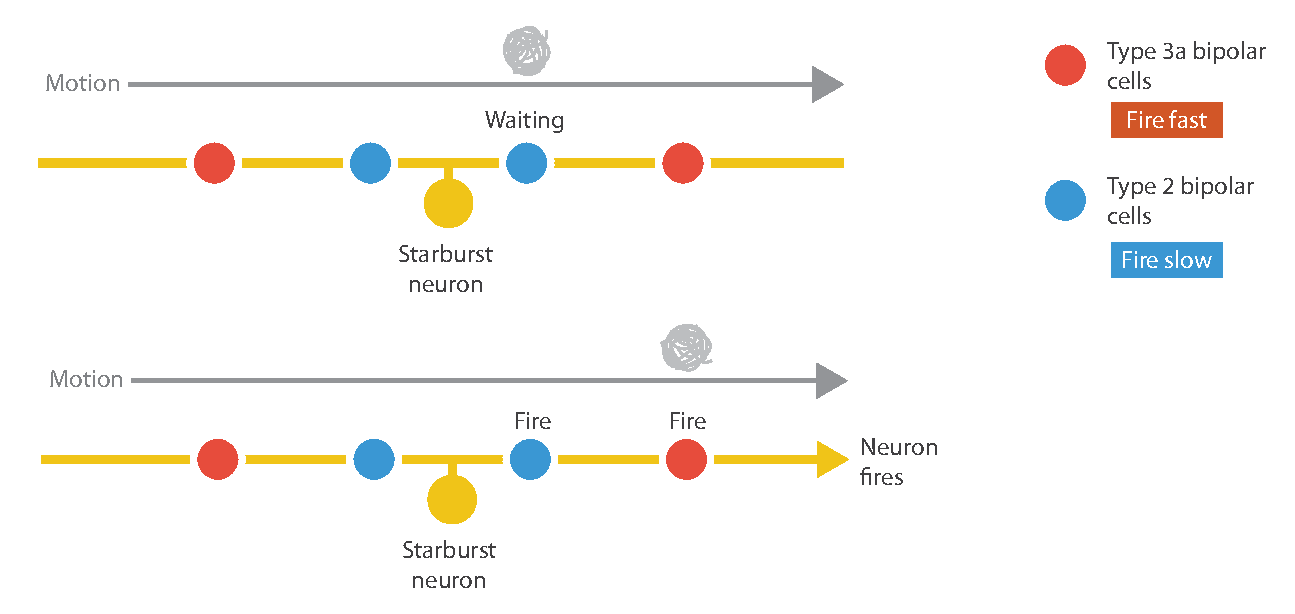
\includegraphics[width=\textwidth]{images/related-work/starburst-neurons}
\caption{Illustration of a starburst neuron (yellow) with two classes of bipolar cells to each side of the neuron. 
Type 3a bipolar cells (red) are farther from the cell body and fire immediately. 
Type 2 bipolars (blue) have a time delay and are close to the cell body.
When motion is detected, both types of cells issue a response, however the starburst neuron fires only when both cells have been activated in a specific order.
In the top image, a ball of string moves across the field of vision illiciting a response from a type 2 bipolar cell, which has a delayed response.
When the ball of string moves over the type 3a bipolar cell, a response is made immediately.
If the response from the type2, followed by the type 3a bipolar cell occurs at the same time, the neuron fires.
Modified from \url{http://blog.eyewire.org/eyewires-first-scientific-discovery-and-nature-paper/}}
\label{fig:motion-neurons}
\end{figure}

Movement is also processed in the visual cortex in both parvo and magno pathways.
These movement sensitive neurons can be classed as one of a number of types: 1) cells that respond to movement irrespective of form. This type can be subdivided in to: a) neurons that respond to motion in any direction; and b) those that respond to one direction; and 2) cells that respond to contour and movement together (almost all directionally selective) \cite{Zeki01021974}.
Similar to how neurons have distinct preferences for a particular orientation, neurons sensitive to motion have a preference for movements in particular directions \cite{maunsell1983functional, dubner1971response, krug2012principles}.
Additionally, these neurons also indicate the depth of the object in 3D space \cite{maunsell1983functional, dubner1971response, krug2012principles}.
As processing moves from the retina to V1, V2, then the middle-temporal (MT) area, there is an increase in the size of the receptive field. 
This represents a change in how processing moves from encoding local contour movement to global object movement.


\subsubsection{Analysis of Surface Properties, Depth and Segmentation}
Contour integration, object motion, and border ownership all contribute to the signals required to determine surface properties, depth, and segmentation. 
There are additional processing steps however using surface properties and depth to assist with object segmentation.

Surface properties (texture, colour, brightness) of an object are calculated through comparison of light arriving in different areas of the visual field. 
What is interesting about colour processing in particular is that even though the amount of available light can vary hugely throughout a typical day, our perception of object colour does not change much. 
This effect is termed ``perceptual constancy'' in the many examples provided by Beau Lotto\footnote{\url{http://www.lottolab.org/articles/illusionsoflight.asp}}. 
A possible explanation to this was given by Zeki who found neurons in V4 that elicit the same response to different illumination wavelengths if the perceived surface colour remains the same \cite{Zeki1983767}. 

Most of the neurons and receptive fields (retinal ganglion cells, LGN, and areas of visual cortex) are signalling contrast, and ultimately contours. 
Receptive field responses are low or non-existent for surfaces with no contrast. 
There are however a small number of neurons that respond to surface brightness, texture, and colour. 
These cells are heavily influenced through context provided by surrounding cells which may alter the perceived brightness. 
For example, in Figure \ref{fig:brightness-change} the brightness of an area surrounding a receptive field can result in perceived changes circle colour, where in fact there was none.
Due to an inequality in the number of neurons representing surface properties versus those dealing with contrast, there is a gap in visual information. 
To overcome this, the visual system performs what is called ``perceptual fill-in'' where the brightness of a surface is calculated from contrast information at the surface boundaries \cite{kandel2012principles}.

\begin{figure}[t!]
\centering

\includegraphics[width=.6\textwidth]{images/related-work/brightness-illusion}
\caption{The two circles are the same colour but the background affects perception with the one on the right appearing brighter due to the decreased brightness of the surrounding areas.}
\label{fig:brightness-change}
\end{figure}

\subsubsection{Depth Perception}
A further operation of this intermediate-level processing step is depth perception, made possible through a number of enablers. 
Information captured in the ocular dominance columns of V1 capture the binocular disparity (differences) created by the two versions of the world perceived by our eyes. 
From this information, a number of further processing tasks take place here to determine depth carried out first by a number of cells in the ocular dominance columns that are selective for objects at different distances.
These cells can be roughly categorised into three types: those with a preference for objects that are near; those with a preference for those that are far away \cite{kandel2012principles}; and those with a preference for objects on the plane of fixation (in between).

Determining depth is a global process that involves many cooperating cells. 
When there is uncertainty about the depth of an object in a group of cells, other cells with no ambiguity can feed information into those regions of uncertainty. 
This process is known as ``disparity capture''.
The global nature of disparity analysis is normally illustrated using random-dot stereograms \cite{julesz1971foundations}. 
These stereograms present what appears as noise to each eye, however when viewed binocularly (with both eyes), embedded shapes become visible\cite{kandel2012principles}.

\subsubsection{The Importance of Context}
The primary function of intermediate processing is to find objects in the scene by integrating the many constituent components of a visual scene. 
We are then able to take these objects and match them to its internal interpretation of previously encountered objects\cite{kandel2012principles}. 

This is not a one-way system and relies on an interconnected network of horizontal connections between cells at the same levels as well as feedback and feedforward system linking all levels of the visual system. 
This process of global integration can be facilitated through application of Gestalt laws about perceptual grouping along with additional high-level features such as attention, expectation, and past experience \cite{kandel2012principles}. 
This is referred to as a ``top-down approach'' and is discussed further in Section \ref{sec:topdown_bottomup}. 

\subsection{High-level Processing}

High-level processing refers both to the stage of visual processing where shapes and surfaces are identified, and in visually guided movement.
Here we focus directly on the former, in object recognition which relates specifically to the parvo pathway where processing continues from the visual cortex by passing surface and form objects to the temporal lobe for identification \cite{kandel2012principles}. 
However information about object movement from the magno pathway will also feed in to object recognition. 
Figure \ref{fig:high-level-processing} provides an overview of the tasks preceding high-level processing as well as the signals that help in object recognition. 
These signals involve:
\emph{working memory};
\emph{categorical linking};
\emph{associative linking};
\emph{signals from other senses} such as sound, smell, and touch;
and \emph{emotional valiance} which relates objects to past emotional events.

\begin{figure}[t!]
\centering
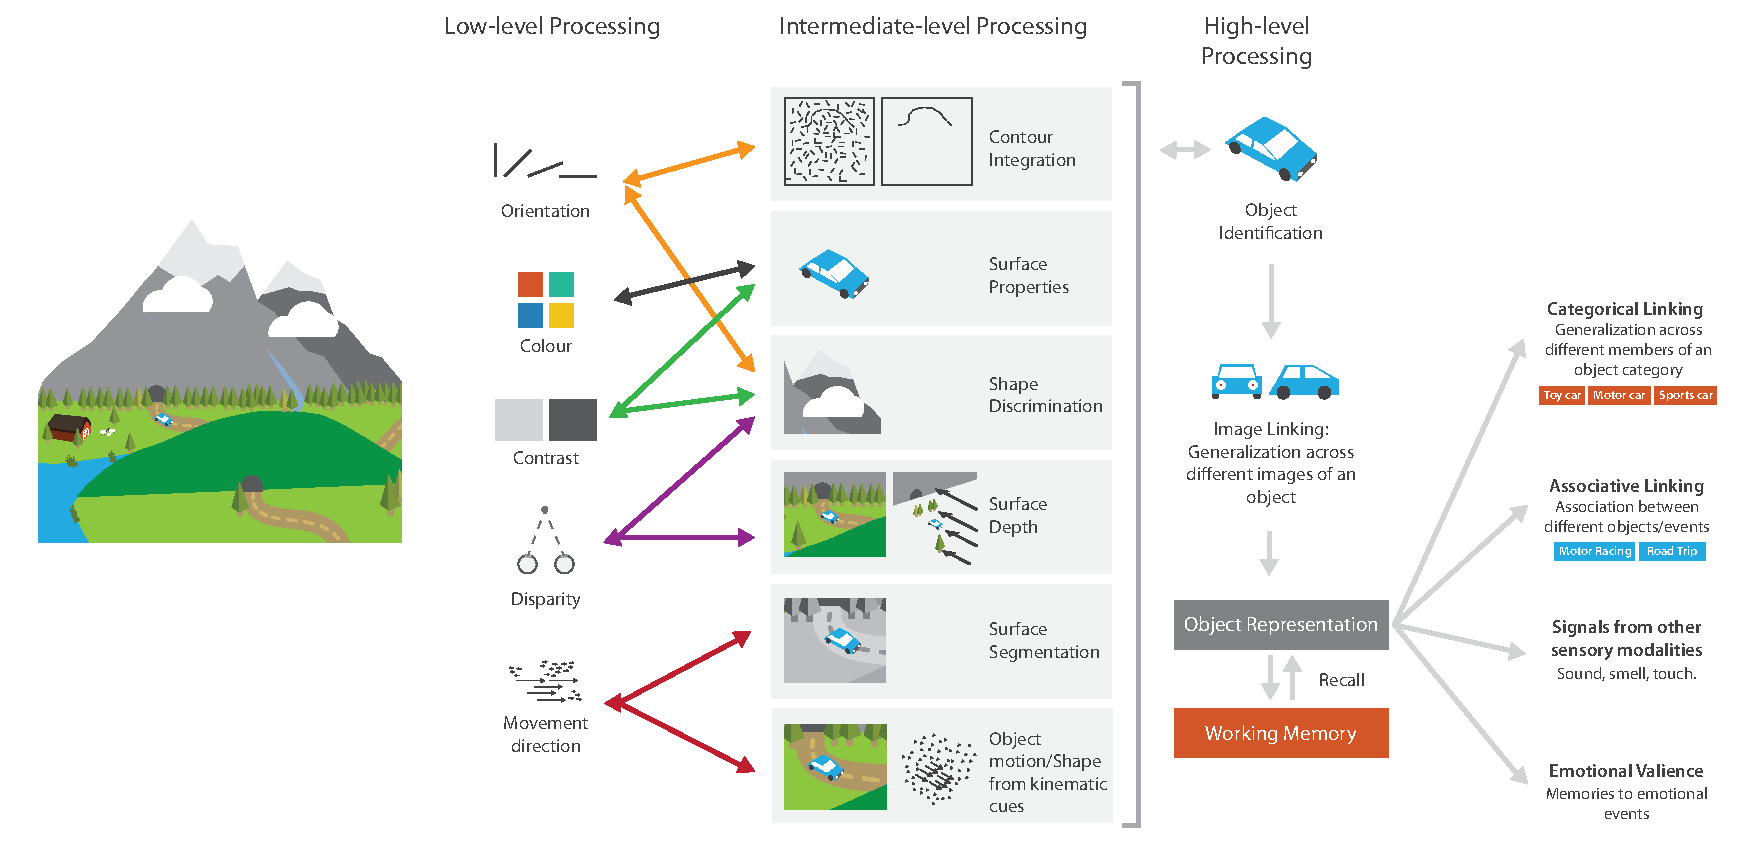
\includegraphics[width=\textwidth]{images/related-work/high-level-processing}
\caption{Flow of processing from low- to high-level processes with a focus on the object identification (parvo) pathway. Adapted from \cite{kandel2012principles}.}
\label{fig:high-level-processing}
\end{figure}

The brain's ability to identify objects is nothing short of amazing. 
Consider that the latest machine learning algorithms struggle to recognise different presentations of the same object. 
Brains on the other hand have been doing this for many thousands of years. 
There are a few areas of the brain responsible for this processing as illustrated in Figure \ref{fig:pathway-object-recognition}. 
The main part however is the inferior temporal cortex at the end of the ventral stream. 
This part of the brain has been clinically shown to be essential to object recognition \cite{kandel2012principles} via the introduction of lesions to this area of the brain in primates and observation of the consequences. 
When lesions were made in the inferior temporal cortex, an effect called \emph{visual agnosia} (coined by Sigmund Freud) was the result where the primates were unable to recognise objects \cite{kandel2012principles}. 
Later research observed this effect in humans and found that visual agnosia had two subclasses: 
\emph{apperceptive agnosia} where patients are unable to copy an object presented to them but they can identify the object \cite{Ferreira01091998}; and 
\emph{associative agnosia} where patients are able to copy the object but do not know what it is\cite{farah1990visual}. 
This research helped in further divisions of the inferior temporal cortex into posterior and anterior regions. 
The posterior region was associated with inability to see objects correctly and the anterior region was associated with assigning meaning to objects.

\begin{figure}[t!]
\centering
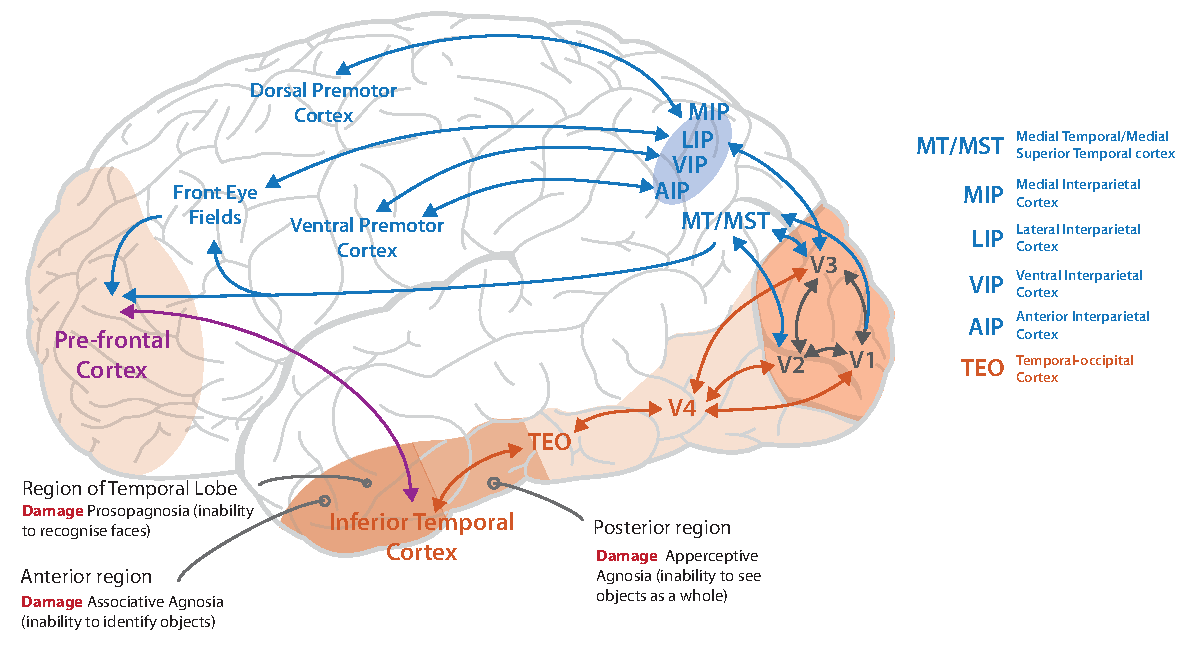
\includegraphics[width=\textwidth]{images/related-work/pathway-object-recognition}
\caption{Side view of the brain showing the object recognition pathway in orange. Adapted from \cite{kandel2012principles}.}
\label{fig:pathway-object-recognition}
\end{figure}

Similar to the early visual processing stages, neurons in the inferior temporal (IT) cortex have receptive fields that respond to distinct stimuli found using electrophysiological techniques. 
The IT is organised into columns with functional specificity to aid identification of particular patterns\cite{tanaka2003columns, kandel2012principles}. 
For example, some populations of neuron have been shown to be solely involved in face and hand detection in monkeys\cite{tsao2006cortical, tsao2008comparing, kandel2012principles}. 
Damage to these populations causes \emph{prosopagnosia} where the ability to recognise faces\cite{kandel2012principles} is lost. Face recognising cells are a population of cells with different preferences to the various ways in which a face may be viewed.
Some cells are shown to respond better to a frontal view of the face whereas others respond better to side profiles \cite{Afraz06, kandel2012principles}. 
These columns which identify different configurations of a face, pencil, computer or other complex forms are referred to as hyper-columns \cite{tanaka2003columns, kandel2012principles}. 
Due to the specificity of such hyper-columns to particular objects and shapes, it is reasonable to assume that the IT cortex is configured based on past experience. 
In other words, our past experiences influence the brain's ability to identify an object and will change in response to new information \cite{kandel2012principles}. 
Gilbert \etal call this process \emph{perceptual learning} \cite{Gilbert2001681}.

Aside from recognising the different configurations of an object in space, there are other problems left to be resolved in the visual system with respect to identifying an object similarly even though these objects may be far away or close by. 
Three populations of neurons have been shown to be involved in aiding a term previously introduced called \emph{perceptual constancy}, where objects can be identified even though they are different sizes (size constancy), have different positions on the visual field (position constancy) or have differences in reflectance (form-cue invariance) \cite{schwartz1983shape}. 

These properties of the object recognition workflow match those posed by Gestalt psychologists who cited \emph{invariance} as a key property of the visual system - the ability to identify items without the need for a precise match to what has been observed previously - referred to as the \emph{prototype} approach by Spoehr and Lehmkuhle \cite{spoehr82} and Franks and Bransford \cite{franks71}.

It should be noted that although a lot of information is known about the structure of the components in the high-level processes, little is known about how perceptual learning occurs, how objects are compared in the brain, how memories are formed, or how interaction between the IT cortex and long-term memory in the hippocampus works.

\subsection{Global and Local Processing}
\label{sec:global_local_processing}

A visual scene is arranged in a visual hierarchy \cite{palmer77, navon77, shor71, love99, kinchla79} where some pieces of information are more accessible than others. 
Large features in a scene such as a building, versus the smaller items that are less easy to see such as the writing on a poster placed on a wall will be more or less accessible to processing by our visual system depending on proximity. 
We will not be able to read the text on a poster for instance from 100 meters away but we will see the outline of the poster.
Global features such as overall shape, colour, \emph{etc.} will be accessible to the visual system from larger distances than local features such as the lines of text on a poster and the key factor is spatial frequency. 
The fovea, which represents the highest resolution are in the visual field has the smallest receptive field and therefore provides the greatest level of detail. Moving further away from the fovea the receptive fields become larger and the detail these areas capture becomes much more coarse \cite{kandel2012principles}.

\begin{figure}[h!]
\centering
\includegraphics[width=\textwidth]{images/related-work/spatial-frequency}
\caption{A) From further away, a letter will not be fully perceptible as a result of the receptive field in the retinal ganglion cells. 
A single letter could be represented by one receptive field which could be interpreted as nothing more than a blurry spot. 
When the letter is viewed up close, each of the local contours that make up the letter 'E' can be covered by individual receptive fields. 
B) Low detail image as would be seen by our visual system by large receptive fields. As we zoom into focus on particular areas, the granularity of the image keeps increasing until we have a fine-grained image. }
\label{fig:spatial-frequency}
\end{figure}

Figure \ref{fig:spatial-frequency} A serves to illustrate how local, or fine details like text or thin lines will not be readable from far away since the receptive field is not small enough to capture local contrast differences. 
Small text would appear as a blur. 
By decreasing the distance from the text, individual lines can be served by more receptive fields. 
The receptive fields provide the contour information used to encode the letter, and this information can then be passed on to higher levels to be further processed. 
Figure \ref{fig:spatial-frequency} B illustrates how global features such as overall shape, colour, and movement are more easily perceived at the overview level than low-level features such as the door outline on the barn. 
Objects such as the barn (red) pop out from the scene and demand our attention for example. 
Pre-attentive processing will be discussed in more detail in Section \ref{sec:popout}.


\subsection{Bottom-Up, Top-Down and Salient-Feature Detection}
\label{sec:topdown_bottomup}

Depending on what we are looking for, our system can be tuned to finding items very quickly whilst ignoring other items. 
If we are not looking for anything in particular, we may process a scene systematically to look for something interesting, or it could be that some items may be more prominent than others due to pop-out and will command our attention. 
A bright red stop sign in a road for example or the flashing lights of a police car. 
This set of possibilities for how we process a visual field can be classified as: 
\emph{bottom-up} where we start at the low-level features of a visualization and build up the entire image progressively\cite{marrvision}; 
\emph{top-down} where we see outlines of shapes, use context, and other high-level information to infer what those outlines correspond to, then look for the local features of those objects we expect to find \cite{lee2003computations}; and 
\emph{salient-feature detection} where items that pop out in a scene draw our attention and we process these items first. 

\begin{figure}[h!]
\centering
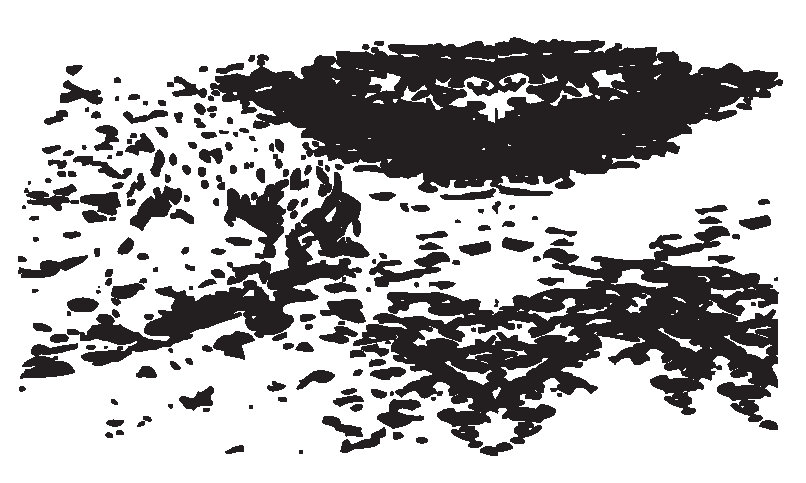
\includegraphics[scale=.55]{images/related-work/top-down-penguin.pdf}
\caption{This image depicts a Dalmation sniffing the ground and is an adaption of that produced by R.C. James and used by Lee \cite{lee2003computations}.
This example serves to show the power of top-down processing where knowledge of the dog in the scene helps in processing, whereas the use of local processing techniques leads to longer search times.
Before knowing a Dalmation is in the scene, viewers often struggle to see it.
This also illustrates a Gestalt effect with the dog shape being apparent even though parts of its body have not been explicitly defined.}
\label{fig:global-dalmation}
\end{figure}

Top-down and bottom-up processing are terms also used to describe the possible computational model the brain follows. 
Do the instructions for processing a scene come from the low-level features and progress through the visual cortex into the high-level object recognition phases (bottom up)? 
Or does it follow an approach where high-level information influences the sensitivity of particular neurons to particular colours, shapes, or textures (top down)? 
The general consensus is that it is not one or the other, but both. 
The visual system consists of a hyper-connected set of neurons with many feedback and feedforward systems enabling information from previous experience, context, and expectations to influence how a scene is processed by the visual processing components in the low- and intermediate- level processing stages of the visual system. 
Gestalt laws, in particular the idea of \emph{emergence} is illustrated in Figure \ref{fig:global-dalmation} where at first glance the subject of the image is unclear. 
For readers unaware of the subject, it could take a fairly large period of time to discover it - there would be a reliance on building the picture from the ``bottom up''. 
When told that the image represents a Dalmatian sniffing the ground, for many viewers, the outline of a Dalmatian will form as a result of our expectations of how a dog should look. 
These expectations tune the visual system to select for particular features (\eg, colours, contours, textures) that represent our inner ``template'' of a dog.
This is ``top-down'' processing.

\subsection{Pre-attentive Processing}
\label{sec:popout}

\begin{figure}[ht!]
\centering
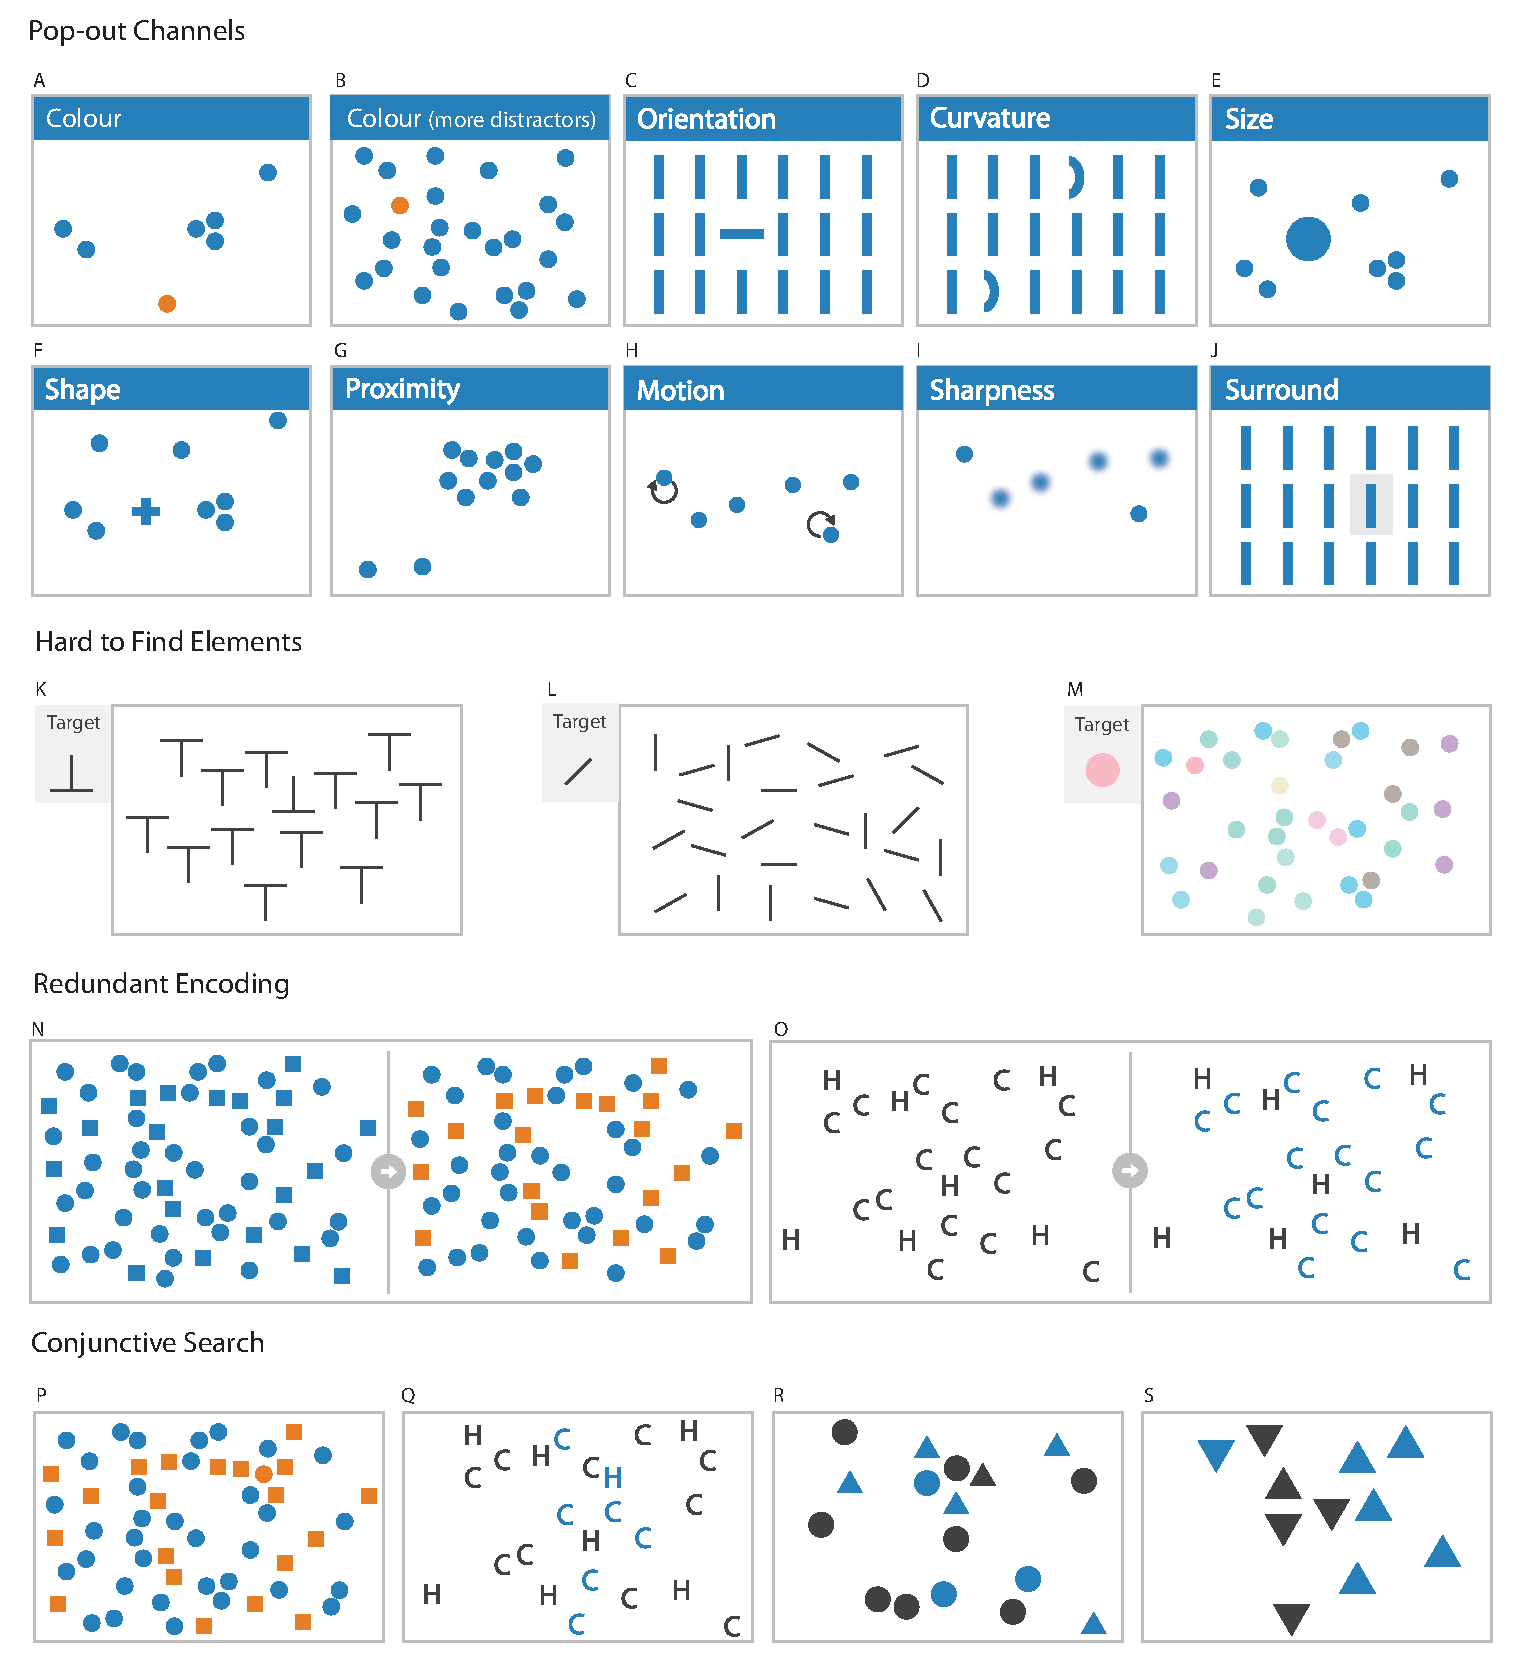
\includegraphics[width=\textwidth]{images/related-work/popout.pdf}
\caption{A to F) Visual channels amenable to pre-attentive processing. 
K to M) Examples illustrating where differences between the search target and distractors is not sufficient to enable fast visual search. 
N and O) The effect of redundant encoding on aiding visual search. 
P to S) Conjunctive search examples where in: 
P, the orange circle is the search target; 
Q, a blue H is the search target;  
R, a black triangle is the search target; and 
S) A upward pointing black arrow is the search target.}
\label{fig:popout}
\end{figure}

In 1988, Anne Treisman \cite{treisman88} first showed that the visual system was somehow able to tune visual attention to find particular objects with specific visual attributes \cite{kandel2012principles, treue1996attentional} in a very small period of time (less than 300 milliseconds).

From this research, a number of visual properties were identified that were shown to be processed by the low-level processing components of the visual system \cite{healey11}.
These properties came to be known as pre-attentive.
As a result of how pre-attentive visual properties visually stand out on a display, the effect is commonly and less formally referred to as the ``pop out effect''.

However the name pre-attentive is now misleading.
Research in 2002 by Kleinschmidt \etal \cite{kleinschmidt2002} showed how top-down feedback loops have been observed to play a role in pre-attentive processing by maintaining attention on a visual object.
This has been studied through observing a visual item gradually becoming visible amongst noise in a busy scene, then observing at what point the item no longer appears, termed ``drop-out''.
There is a difference in the points at which the visual item pops out and when it drops out \cite{kleinschmidt2002}. 
Kleinschmidt \etal found that drop-out occurred at a lower level than pop out occurred.
This effect is called \emph{hysterisis}.
Using fMRI with human participants, Kleinschmidt \etal \cite{kleinschmidt2002} were able to detect enhanced activity in the temporal, parietal, and frontal cortex that correlated with the preservation of the pop-out effect.
This study provides evidence of top-down processes being important in the pop-out phenomena.
Nevertheless, the term pre-attentive continues to be used to refer to visual items that can be found rapidly in a display \cite{healey11}. 


As shown in Figure \ref{fig:popout}, almost all visual channels support pre-attentive processing.
The speed at which these variables pop out however is not always the same.
The visual channels that perform best (derived from the psychology literature) can be ordered as colour $\prec$ size $\prec$ shape $\prec$ orientation (\eg, \cite{williams67,quinlan87,ropinski11}) where symbol $\prec$ reads as \emph{precedes}.
An interesting property of the pre-attentive processing is that it is not bound by the number of distractors in the scene\cite{ware13}.
In Figures \ref{fig:popout} A and B for example, the number of blue circles does not impact search on the red circle.

The effect of pre-attentive processing may be increased or decreased depending on how variables are combined with each other.
To increase, a technique called redundant encoding can be used where the visual representation of items in a display are encoded with two or more non-overlapping visual channels.
Figures \ref{fig:popout} N and O show this effect in action.
In Figure \ref{fig:popout} N, shape is used to solely distinguish two groups.
With the addition of colour in Figure \ref{fig:popout} O, the separation is more clear with one group represented with blue circles and the other with orange squares. 

To decrease or remove the ability to pre-attentively process a scene, one may reduce the visual distance, or noticeable difference between visual items in the display.
For example, in Figure \ref{fig:popout} B we have two hues with a large noticeable distance that lend themselves to fast visual search.
In Figure \ref{fig:popout} F we have seven colours within overlapping colour hues that have a much smaller noticeable difference between them.
In this example, visual search becomes more time consuming and erroneous.

Additionally, Figures \ref{fig:popout} C and L show the same effect for orientation.
In Figure \ref{fig:popout} C there are two orientations with a large difference.
Figure \ref{fig:popout} L shows an example with five orientations where finding the line with the correct orientation becomes very difficult.

Finally, by adding complexity to the search requirements, the speed of visual search will be further reduced.
In single feature detection, a participant in an experiment generally looks for a H amongst Cs. 
As found by Navon, this search environment lends itself to parallel processing so the distractors and targets can be processed simultaneously \cite{navon77}.
Where there are overlapping search criteria, this is termed ``conjunctive'' search which does not lend itself to parallel processing \cite{navon77}.
Take Figure \ref{fig:popout} Q where we search for a blue H amongst black and blue Cs and black Hs.
The visual system must first look for the blue items, which gives a mixture of Hs and Cs, then look for the Hs.
Due to the combination of features to be searched on, conjunctive search is generally slower than single feature detection \cite{quinlan87}.
This is a process illustrated in Figure \ref{fig:visual-search}.

\begin{figure}[t!]
\centering
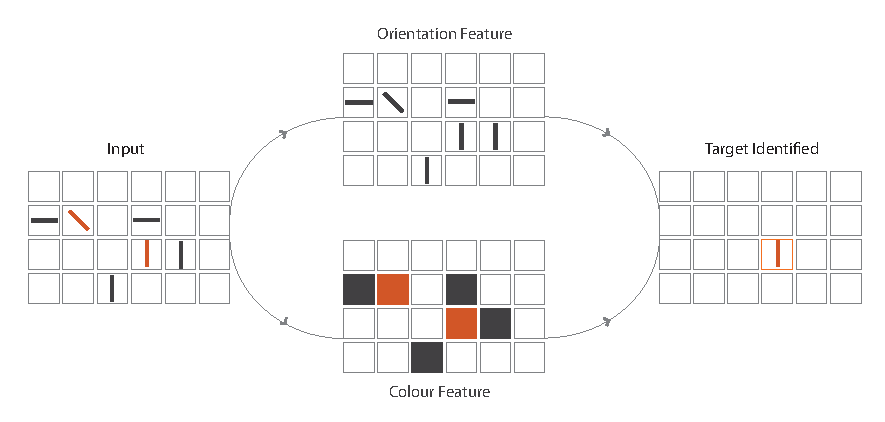
\includegraphics[width=.8\textwidth]{images/related-work/visual-search.pdf}
\caption{An illustration of how feature detection is said to work. This process is often posed as either a parallel or serial function and shows how in a visual scene of orange and grey lines how one may pick out the vertical orange line through combining the results of the orientation and colour feature searches together.} 
\label{fig:visual-search}
\end{figure}

The neurophysiological explanation for why visual elements in a display are available of pre-attentive processing or ``pop out'' is largely cited as being caused by contrast differences, and a top-down feedback loop that maintains attention on the concept that has popped out.
Contrast differences have been shown in centre-surround cells in V1 that select for orientation by Schmid and Victor \cite{Schmid2014}, illustrated in Figure \ref{fig:orientation_rf}.

\begin{figure}[t!]
\centering
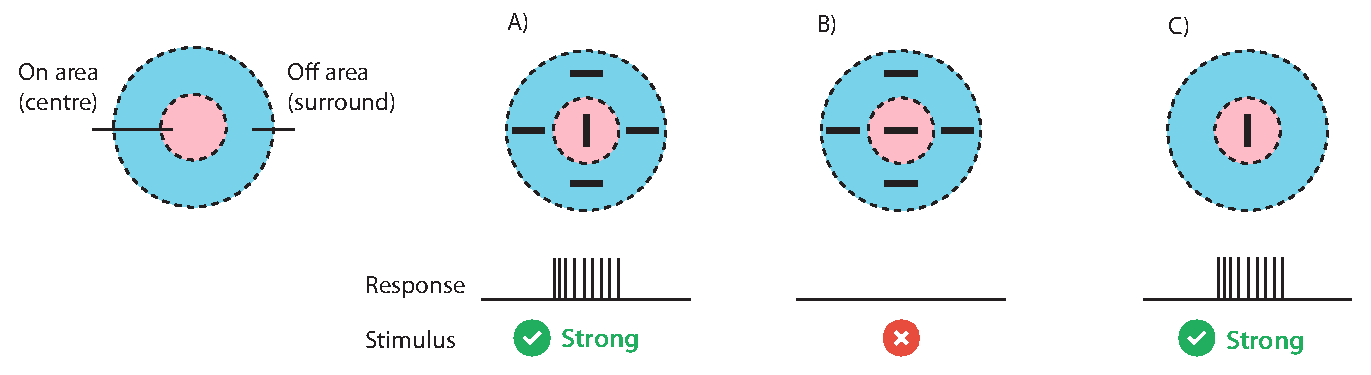
\includegraphics[width=\textwidth]{images/related-work/orientation_rf.pdf}
\caption{Based on those reported by Schmid and Victor \cite{Schmid2014}. A) With the orientation in the centre different from the surround, a strong response is recorded from the cell.
B) When orientation is the same in the centre and surround, no response is output. C) With an orientation detected in the centre but not in the surround, a strong response is output.} 
\label{fig:orientation_rf}
\end{figure}

When the orientation in the centre of the receptive field differs from that in the surround, the neuron response is high (Figure \ref{fig:orientation_rf} A).
If the orientations are the same, there is no response (Figure \ref{fig:orientation_rf} B and C).
Further studies would be needed to confirm similar receptive fields for colour and position for example, and at the higher levels of the visual processing pipeline, such as in V4 which deals with more complex forms.


\subsection{Integral and Separable Dimensions}
\label{sec:channel-composition}

 \begin{figure}[t!]
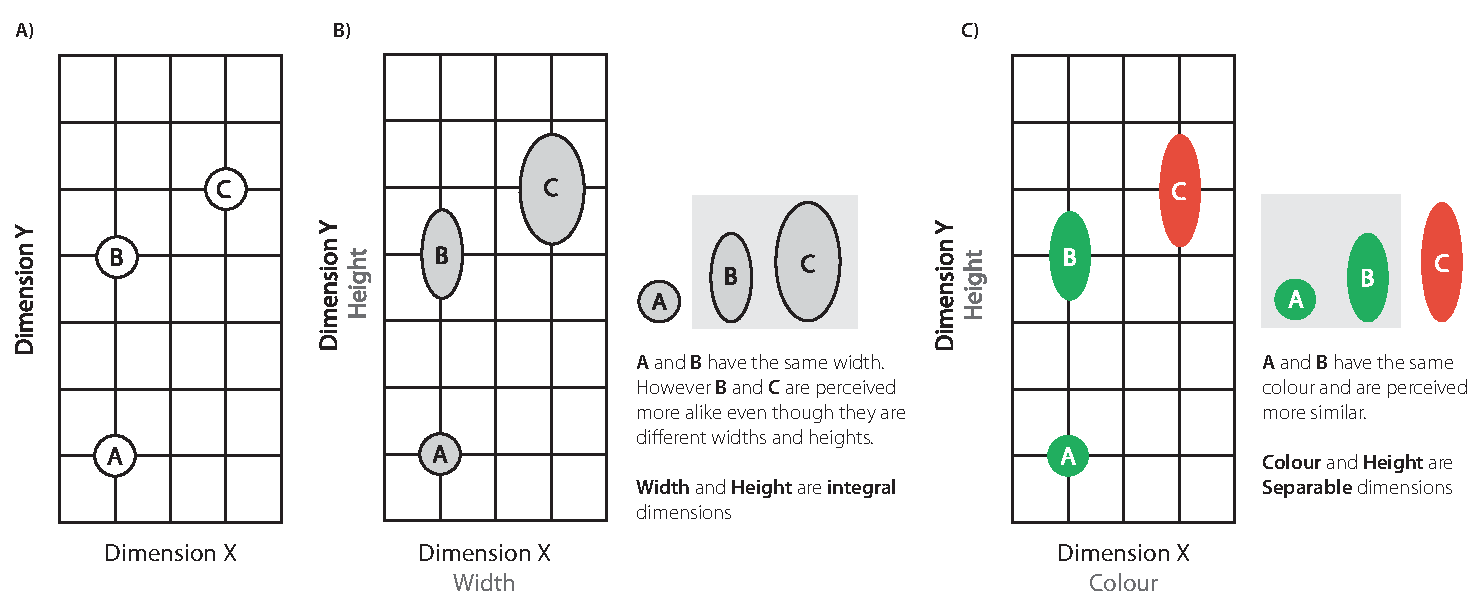
\includegraphics[width=\textwidth]{images/related-work/integral_separable}
\caption{Some examples from Ware \cite{ware13} to explain integral and separable dimensions. A) Ware \cite{ware13} used this grid to help designers think about separability of dimensions. B) Replacing dimensions X and Y with width and height respectively, we can see that even though A and B have the same width, B and C are perceived more similar. These dimensions are integral. C) With colour replacing width, A and B are now perceived more similar, which is the desired effect. These dimensions are separable}
\label{fig:integral_separable}
\end{figure}

The theory of integral and separable dimensions was developed by Garner \cite{garner1974processing} in his book \emph{The processing of information and structure} based on a number of experiments by Attneave\cite{attneave1950dimensions}, Garner and Felfoldy \cite{garner1970integrality}, and Shepard \cite{shepard64}.

\emph{Integral} dimensions are perceived together instead of independently. 
As an example, Figure \ref{fig:integral_separable} B shows some simple glyphs as an ellipse whose width is mapped to dimension X and height is mapped to dimension Y of some data record. 
Even though glyphs A and B are more similar with the same width, it is B and C that are visually more similar. 
The overall shape of the ellipse is perceived rather than its individual parts (width and height).  
Previous research by Attneave \cite{attneave1950dimensions}, Shepard \cite{shepard64}, Krantz and Tversky \cite{krantz75}, and Handelt and Imai \cite{handelt72} found that integral dimensions exhibit what is known as a Euclidean distance (shortest path) defined as $\sqrt{d^2_a + d^2_b}$.
This has been recently validated by Demiralp \etal \cite{demiralplearning} in a large crowd sourced experiment.

\emph{Separable} dimensions are perceived independently.
This means, that converse to the integral dimension example, the individual components of the glyph can be perceived. 
In Figure \ref{fig:integral_separable} C, an ellipse glyph has its colour mapped to dimension X and height mapped to dimension Y. 
This has the effect of making glyphs with the same value of dimension X more similar, and can therefore be selected from the visual scene more easily.
Separable dimensions exhibit a city-block distance where distance is defined as $d_a  + d_b$ \cite{burns78,shepard64}.
This has also been recently validated by Demiralp \etal \cite{demiralplearning}.


What is important to note here is that defining a pair of visual channels as integral and separable is not always a binary classification. 
Both classes are on a continuum as shown in \ref{fig:integral_separable_continuum} where some pairs, such as width and height are fully integral pairs, whereas group location and colour are fully separable pairs. 
Additionally, as Ware states, the theory is very simplistic, and has many exceptions to the rule \cite{ware13}.
However, it does have merits as a design principle and can help designers avoid well-observed problems with the use of particular combinations of visual channels to encode data attributes.

 \begin{figure}[t!]
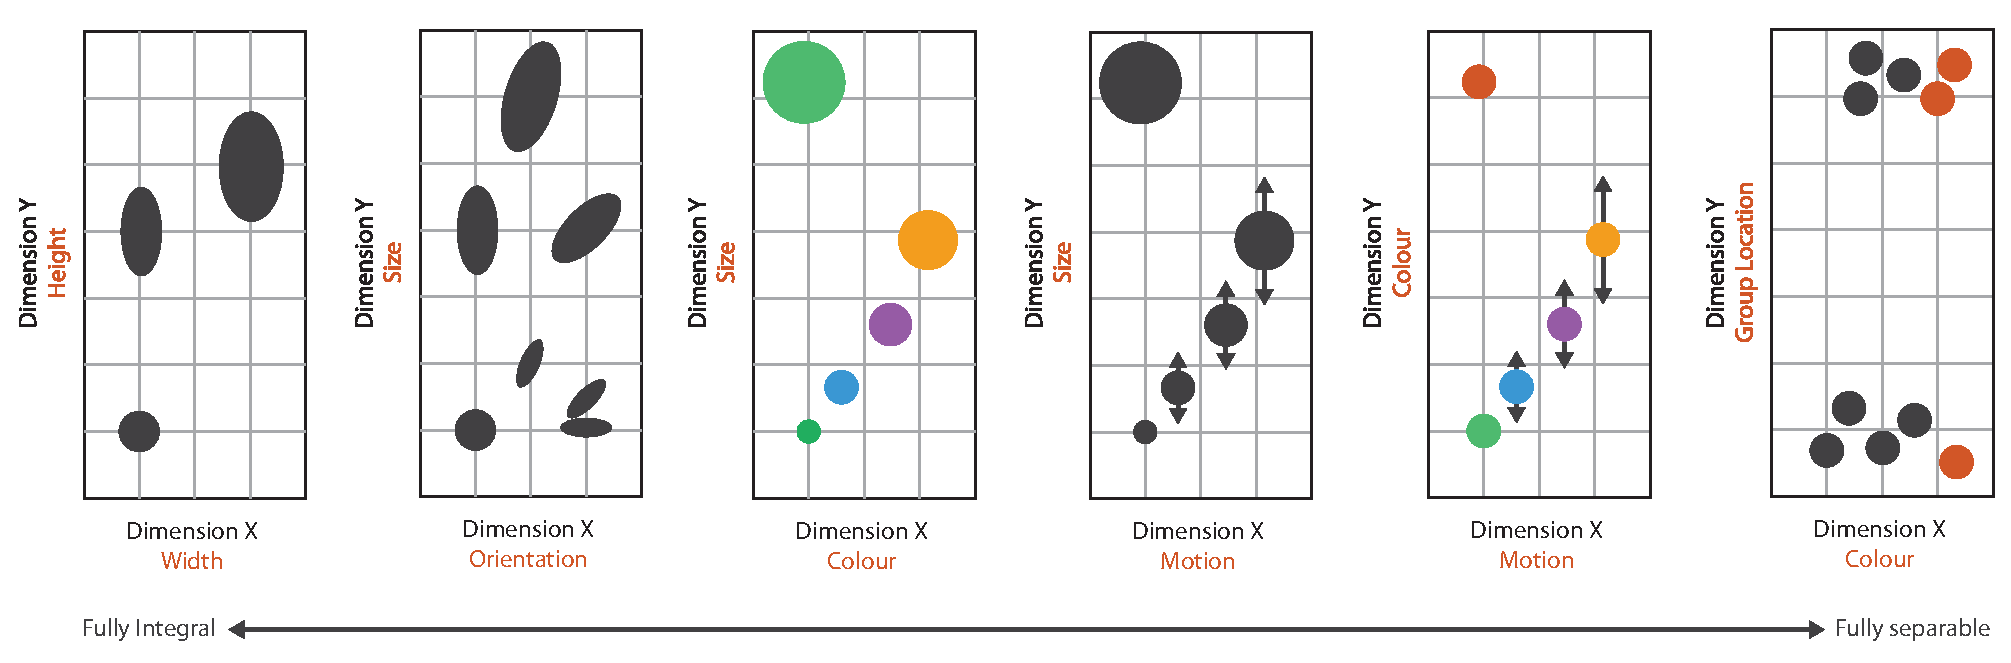
\includegraphics[width=\textwidth]{images/related-work/integral_separable_continuum}
\caption{Adapted from examples by Ware \cite{ware13} to show how pairs of dimensions may not by fully separable nor fully integral, but somewhere on a continuum.}
\label{fig:integral_separable_continuum}
\end{figure}

A full neurophysiological explanation for channel composition is not fully known.
However, a possible explanation lies in how the populations of neurons that process features may have an effect on integrality and separability of the channels they encode.
For example, Garner found that orientation is perceived independently of colour \cite{garner2014}, and Hubel, Wiesel and Livingstone found that shape and orientation are encoded by separate neural populations \cite{hubel1968, livingstone1988}.
Conversely, as stated by Garner \cite{garner2014}, Ganel \etal \cite{ganel2006}, and Drucker \etal \cite{drucker2009}, integral dimensions such as width and height are encoded by overlapping neural populations.

As previously stated by Kandel \etal, the size of the receptive field grows as one progresses through the visual system \cite{kandel2012principles}.
Features coded by overlapping neural populations (such as width and height) are likely to be merged later in the visual processing step and perceived and stored in working memory as an integrated object.
On the other hand, features coded by distinct neural populations will not be merged in to one, and will be stored in working memory as separable objects, and so will be perceived independently.

\subsection{Summary}
In this section we presented the building blocks of a visualization (visual channels), their power in representing particular types of data, and how these visual channels are processed by the visual system.
Additionally, we have discussed concepts of particular importance in glyph design including global and local processing, how feedback between multiple parts of the visual system can affect perception (bottom-up, top-down, and salient feature detection), pre-attentive processing, Gestalt effects, and integral/separable dimensions.

The goal of this section is to bring attention to what is already known from the cognitive sciences and attempt to explain why these effects happen.
Moreover, we aim to use the information presented here to guide users in the design of glyphs.



\section{Glyphs and Glyph-Based Visualizations}
\label{sec:relwork_glyphs}
The word \emph{glyph} is derived from the Greek word \emph{glyph$\bar{e}$} which means carving.
From the Palaeolithic age (18,000 BC) and their use of cave paintings, to the Neolithic age with petroglyphs (``stone carving''), pictures have been used to tell a story using symbols to depict particular events, objects, places, and activities (pictograms) or ideas (ideograms).
What is interesting about such pictorial approaches to story telling and communication is that there is a great intersection between visual language across vast different geological areas \cite{Eliade1991}.
This finding would indicate that symbols are key to the human conceptual system and that many of these symbolic representations are ``hard-wired'' in the brain \cite{Borgo:2013:EG,Eliade1991}.
Additionally, Egyptian hieroglyphs involve a more complex set of glyphs that pictorially represented not just ideas (ideograms), but also phonetics, and morphemes (the smallest grammatical unit of language).
The Chinese language with approximately thirteen dialects looked to pictograms and ideograms to solve communication problems between populations from different areas.
Perhaps the pictorial representations are not so clear in modern Chinese, however as illustrated in Figure \ref{fig:chinese-evolution}, this visual language has evolved from very metaphoric representations to their more abstract representations used today.
An additional feature of the Chinese language is how glyphs can be combined logically to mean something new, \eg, \emph{human being} can be combined with \emph{two} to mean \emph{humane}. 

\begin{figure}[b!]
\centering
\includegraphics[width=.7\textwidth]{images/related-work/glyphs/chinese-pictograms}
\caption{The evolution of pictorial representations adapted from \url{http://www.ocf.berkeley.edu/\~wwu/chinese/handout.html} show how pictograms have evolved into more abstract representations over time with the use of different script styles.}
\label{fig:chinese-evolution}
\end{figure}

These examples show that glyphs are not a new concept, they have been used for many thousands of years to communicate across cultures and languages.
Even now they are used in language and are prevalent in human-computer interaction via metaphoric icons representing functions. 
The definition of glyphs by Borgo \etal \cite{Borgo:2013:EG} as \emph{small visual} objects that have a \emph{meaning}, involve \emph{learning}, and are often \emph{metaphoric} bridges the definitions of glyphs in ancient Chinese writing, Hieroglyphs, and Petroglyphs to the definition of glyphs used in visualization.
The primary difference is in that instead of solely representing ideas or physical objects, glyphs for multivariate data exploration depict qualitative and/or quantitive attributes of data records using combinations of visual channels \cite{Borgo:2013:EG}.
The result should be a \emph{small, visual} object that encodes multiple dimensions (has \emph{meaning}), and requires some \emph{learning} like those glyphs shown in Figures \ref{fig:glyphs-simple-complex} A and B.
Figure \ref{fig:glyphs-simple-complex} A shows a relatively simple glyph design encompassing five dimensions: wind speed, wind direction, temperature, and location (X and Y position).
The use of metaphor, in colour for temperature, arrow orientation for direction, proximity for speed, and position for location makes this glyph intuitive to decode. 

A more complex example is given in Figure \ref{fig:glyphs-simple-complex} B) created by Duffy \etal \cite{Duffy:2014:TVCG} who encode twenty-three data attributes in a single glyph.
The overall objective of this work is the creation of a summary visualization to reduce the need for domain experts to watch and re-watch videos.
Each glyph is used to summarise one second intervals of sperm video data.
These sperm glyphs are viewed with respect to their spatial setting with each glyph representing one second of activity for each sperm cell.
Domain experts can easily get an overview of the movement of the cell and its detailed properties through one image.

Both examples have illustrated the special ability of glyph-based visualization to preserve spatial information that would not be possible using parallel coordinate plots or scatter plot matrices.
Glyph placement strategies have been covered in detail by Matt Ward's \cite{ward02} excellent survey.
This work provides a comprehensive taxonomy of different layout algorithms in 2D or 3D space: data-driven (raw); data-driven (derived); and structure-driven.

\begin{figure}[t!]
\centering
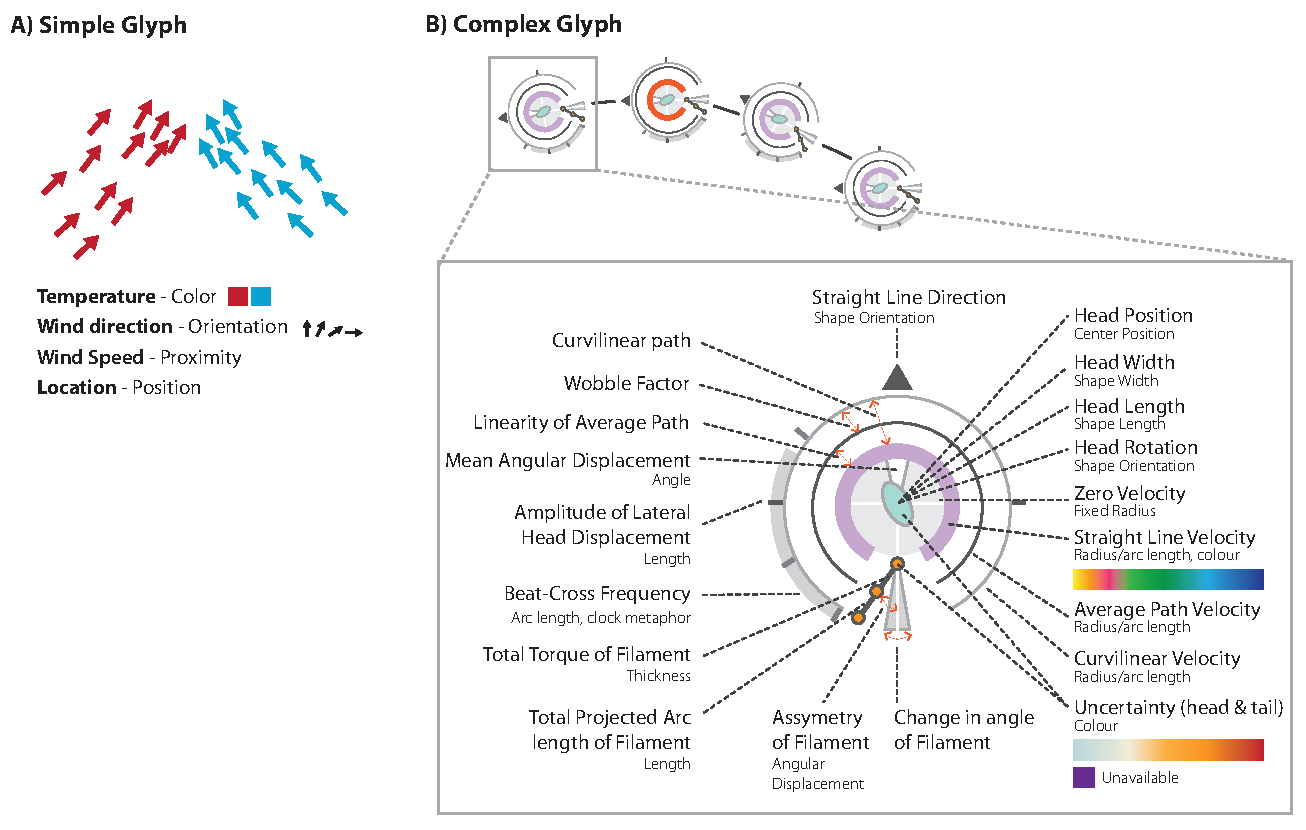
\includegraphics[width=\textwidth]{images/related-work/glyphs/glyph-simple-complex}
\caption{A) A relatively simple glyph for display of weather with five dimensions: wind speed, wind direction, temperature, and location (X and Y position). B) A more complex glyph with twenty-three dimensions by Duffy \etal depicting the attributes of sperm cells \cite{Duffy:2014:TVCG}.}
\label{fig:glyphs-simple-complex}
\end{figure}

These examples illustrate the power of glyphs in three ways: \textbf{1) multi-dimensionality} - glyphs can represent a large number of dimensions; \textbf{2) compactness} - they are able to ``compress'' a large amount of information in to a small space; and
\textbf{3) spatial preservation} - the ability to keep spatial information whilst overlaying more information.


\subsection{Glyphs and their Visual Encoding}
\label{sec:mapping-glyph-data}

Creating a glyph is often more involved than randomly assigning a data attribute to shape, colour, texture, size, or orientation.
Similar to visual signs or fonts, the design of a glyph set is in essence a visual coding scheme \cite{Borgo:2013:EG}.
Like all coding schemes, a well-designed glyph-based visualization can facilitate efficient and effective information encoding and visual communication \cite{Borgo:2013:EG}. 
A bad glyph design on the other hand may lead to ambiguity and confusion. 
Examples of good and bad coding schemes are shown in Figures \ref{fig:signs-code} A, B and C with examples based on letter discrimination and road sign design. 

Figure \ref{fig:signs-code} A shows how font choice, in essence a coding scheme, is important in the interpretation of letters. 
Using the \emph{Myriad Pro} font, many letters will not be ambiguous, such as \emph{a}, \emph{b}, and \emph{c}, however some letters will introduce ambiguity.
In the case of Illinois, the uppercase \emph{i} is not distinguishable from the lower case \emph{L}. 
While this ambiguity can be removed via context and past experience (\eg, knowing how to spell Illinois), it is a problem when previous context is not available, as is the case when learning another language. 
Change the font to \emph{Courier New}, and the ambiguity has been removed. 
Similar difficulties may arise when comparing \emph{\emph{S} and \emph{5}}, \emph{\emph{B} and \emph{8}}, \emph{\emph{A} and \emph{4}} for instance.

\begin{figure}[t!]
\centering
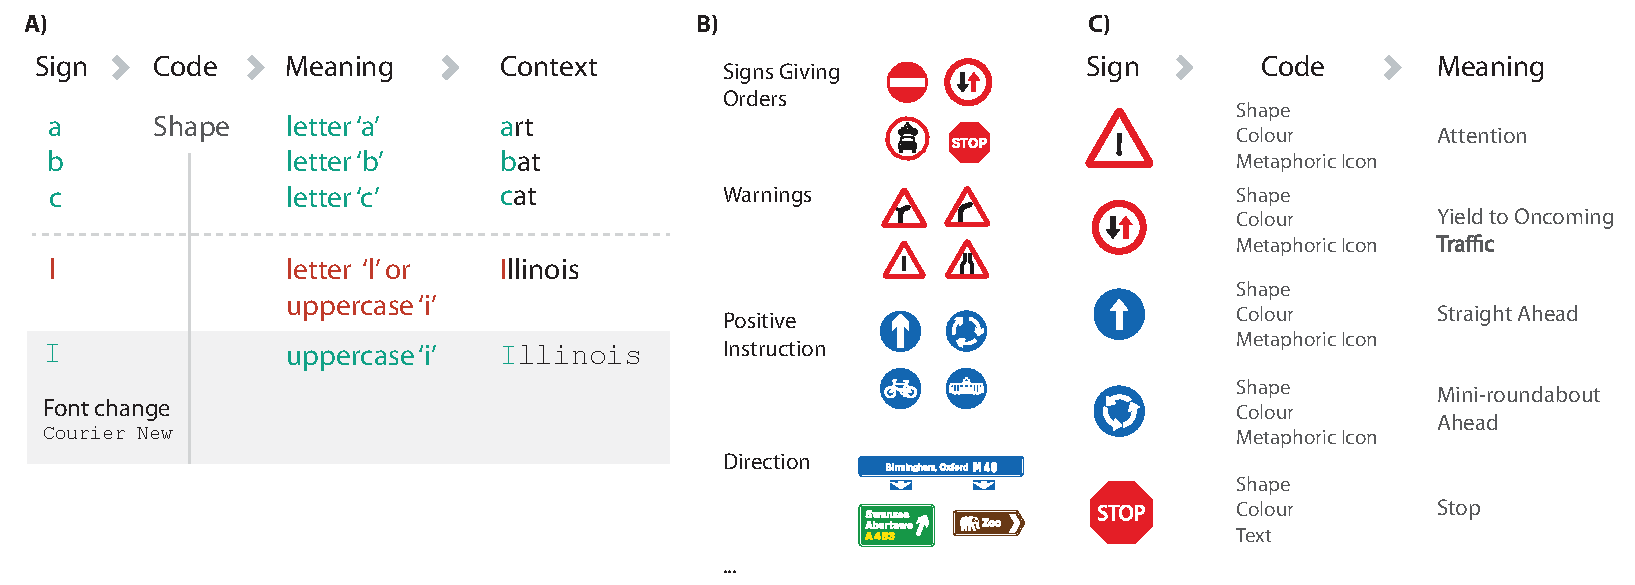
\includegraphics[width=\textwidth]{images/related-work/glyphs/signs-codes}
\caption{A) Letters are simply shapes that we assign meaning to. 
The code for creating such a shape is a particular font. 
With certain fonts, the differences between the letters is not sufficient, making it hard to find the meaning of a particular code. 
In this example, an uppercase \emph{i} can be confused with an \emph{l} (lower case \emph{L}) using the \emph{Myriad Pro} font, but is communicated more clearly using a font such as \emph{Courier New}. 
B) Road signs of the United Kingdom share some clear characteristics in different categories to make it more easy for drivers to visually select for particular pieces of information. 
C) Each sign is encoded with some information, normally pictorially to aid use by visitors from other countries and to encourage adoption as a standard across countries.}
\label{fig:signs-code}
\end{figure}

Figure \ref{fig:signs-code} B presents some classes of road signs for the United Kingdom. 
Road signs have been used for many years and have been iterated on heavily since the late 1950s \cite{kinneir1980words}. 
These iterations were made to ensure that drivers are able to find the information they are looking for (directions, warnings, \emph{etc.}) and that the most important messages are immediately visible to drivers (\eg, warnings and orders). 
If all road signs had the same general design, it would be difficult for drivers to select those signs that are important for safety from those that merely indicate the next service stop. 
If every road sign was too different from the next, drivers would have too much to remember. 
Designed by Kinneir and Calvert, U.K. road signs presented a solution in the form of categories of signs related to the type of message being communicated. 
These road signs had the additional requirement of being universally interpretable which brought challenges in ensuring visitors from other countries could recognise the signs and learn them quickly. 
This is similar to the requirement of the Chinese language to be readable by speakers of all thirteen dialects. 
This was enabled through adoption of European road signage protocols where circles indicated \emph{orders}, triangles indicated \emph{warnings}, and rectangles indicate \emph{information}. 
Colour was used carefully to add further discriminability (termed as \emph{redundant encoding}) to classes of signs, \eg, red for important warnings or orders, and blue for information signage. 
Finally, heavy use of text in previous road signs made it difficult for drivers from other countries to understand. 
Calvert introduced the use of pictograms instead of text where possible to refer to services, museums, men at work, and so on. 
This collective use of categories, shape, colour, and pictograms gave rise to the highway code, a visual language for the road in place since 1958 and a fine example of good glyph design.

Figure \ref{fig:signs-code} C illustrates a \emph{sign - code - meaning} relationship for road signs. 
In these examples and those in Figure \ref{fig:signs-code} B one may see that shape and colour play a large role in determining the type of sign while metaphor is used as much as possible to provide the internal shape. 
Metaphor is very important in the creation of signage due to the lower overhead required to remember what a sign means. 
Too many abstract shapes and colours would place a large cognitive load on anyone trying to decipher one of these codes. 
Additionally, important road signs such as \emph{stop} and \emph{no entry} are different from other signs under the \emph{giving orders} category due to their importance on the road. 
Not stopping at a junction or going up a one way street have the potential to cause great damage. 
Therefore these signs have a full red background which has a metaphoric relationship with \emph{danger}, with white text/shapes in the middle. 

\subsection{Glyph-based Visualizations}
\label{sec:glyph-examples}
From Chernoff faces \cite{chernoff1973use}, a generic glyph technique using facial attributes to represent data, to more application-specific glyphs such as the sperm glyphs by Duffy \etal \cite{Duffy:2014:TVCG}, glyphs have been used as a visualization technique across many diverse areas. 
Matt Ward provided an excellent summary of different types of glyphs in his 2002 paper \cite{ward02}.
The glyphs he identified, summarised in Figure \ref{fig:wardglyphs} included: profile glyphs (using height and colour of bars); star glyphs; Anderson/metroglyphs; stick figures; trees; auto glyphs; boxes; hedgehogs; Chernoff faces; arrows; polygons; dash tubes; weathervanes; circular profiles; colour glyphs; bugs \cite{chuah1998}; and wheels \cite{chuah1998};.

\begin{figure}[h!]
\centering
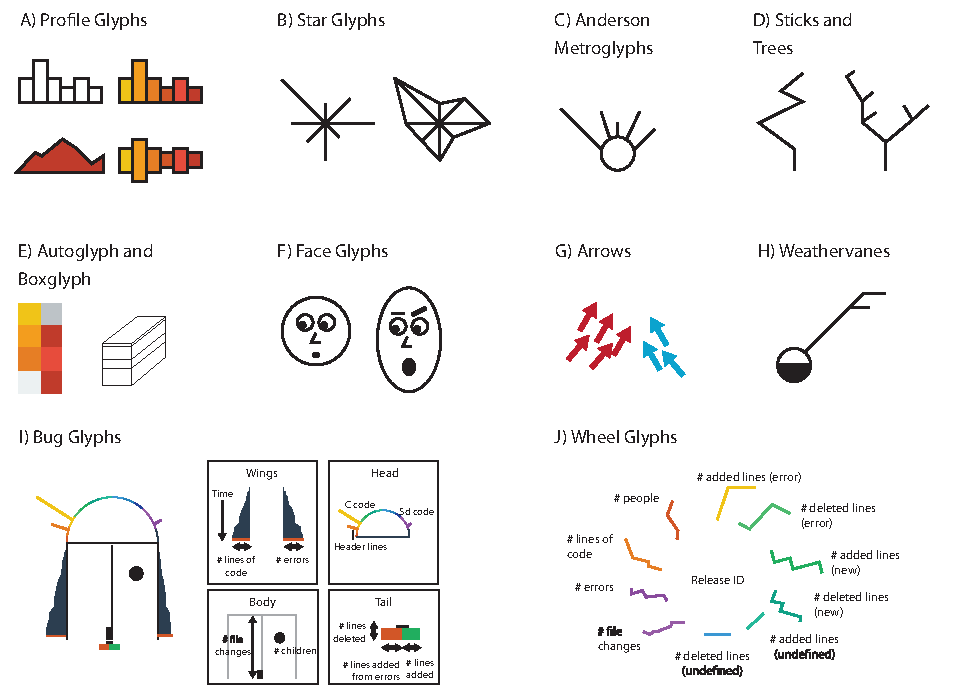
\includegraphics[width=\textwidth]{images/related-work/glyphs/glyphs_ward}
\caption{Some glyph examples from Ward \cite{ward02} with A) variations on profile glyphs; B) star glyphs; C) metroglyphs; D) stick and tree glyphs; E) Autoglyph and box glyphs: F) face glyphs (Chernoff faces); G) arrow glyphs; H) weathervanes; I) bug glyphs; and J) wheel glyphs.}
\label{fig:wardglyphs}
\end{figure}
 
Additionally, here we summarise the contribution glyphs have made in medical, event, geo-spatial, software management ,and search result visualizations.

\textbf{Medical visualization} has benefited from glyph-based visualization. 
They have been used for:
cardiac data by Ropinski and Preim \cite{ropinski08,ropinski11}, Oeltze \etal \cite{oeltze2008glyph}, and Meyer-Spradow \etal \cite{meyer2008glyph};
brain imaging, specifically (functional) magnetic resonance imaging ((f)MRI) by Tory \etal\cite{tory2001visualization}, Westin \etal \cite{westin02processing}, Zhukov and Barr \cite{zhukov2003heart}, Kindlmann \cite{kindlmann2004superquadric}, and Basu \etal \cite{basu2006rician};
and computerised tomography (CT) by Ropinski \etal \cite{ropinski2007surface}. 
A typical use case for glyphs, as identified by Ropinski and Preim, is where data from multiple sources (CT, positron emission tomography (PET) and MRI) are combined \cite{ropinski08}. 
MRI and CT data provide a detailed, high-resolution view of the anatomical structure whereas PET scans show cells that are metabolically highly active with the inclusion of glucose in the PET tracer along with a radioactive label. 
Tumour cells are typically more metabolically active than normal cells; therefore their need for energy, and therefore glucose is increased.
PET scans show these areas of activity and are pointers towards cancer sites. 
Additionally, Duffy \etal \cite{Duffy:2014:TVCG} created a glyph-based summary of videos representing sperm movement. 
For a more in-depth survey of glyph use in medical visualization, see Ropinski and Preim's recent surveys on glyph use in medical visualization \cite{ropinski08,ropinski11}.

\textbf{Event/activity visualization} is a growing area of research where glyphs are becoming a widely used technique. 
Botchen \etal \cite{botchen08ActionBasedVideo} used glyphs to create summaries of video surveillance systems. 
Such glyphs encode position of objects, size, type of action, and relation with other objects as well as statistical information about uncertainty of the analytics algorithm. 
Pearlman and Rheingans \cite{pearlman08} used glyphs to represent nodes of a computer network where different types of network events and their frequency are represented using pie charts. 
These pie charts can be nested within each other to encode changes over time. 
Legg \etal \cite{Legg:2012:CGF} used metaphoric glyphs for annotation of rugby match videos to encode information about the type of event (metaphoric pictograms), the players involved (boxes with player shirt numbers), and the team involved (colour). 

\textbf{Geo-spatial visualization} is an area where glyphs have long been used to overlay information on maps. 
In 1855, Dr. John Snow was one of the first users of glyphs in geo-spatial visualization when he used the famous map of London overlaid with cholera incidents to communicate the relation between water pumps and the location of cholera victims \cite{snow1855mode}. 
His simple glyph made use of stacked rectangles to indicate the number of incidences and position to show location. 
More recent examples include MacEachren and Brewers \cite{maceachren1998visualizing} use of colour and texture to represent the reliability of health care statistics data. 
Figure \ref{fig:glyphs-simple-complex} A shows a simple glyph visualization for weather data where the location of each arrow represents a measurement at a particular geo-spatial location. 
Weather visualizations make good use of visualization to overlay information on top of maps such as rain fall, cloud cover, temperature, and so on. 
Noodles from Sanyal \etal \cite{sanyal:2010:NTEU} use glyphs to show uncertainty in weather data. 
Ware and Plumlee \cite{Ware01072013} show how glyphs can be used to redesign weather displays.
\emph{SkyScope} by Coelho and Low\cite{coelhoskyscope} and \emph{AWE} by Spirkovska and Lodha \cite{spirkovska2002awe} use glyphs to provide pilots with weather forecasts over time including temperature, cloud cover (at different heights), precipitation, and wind direction. 
\emph{SWIM} by Lundblad \etal \cite{lundblad2009interactive} is a decision support system for use by shipping companies to plan ship routes based on weather data. 
Ships are illustrated by glyphs and their route is illustrated via a line. 
Wind speed and direction are shown via glyphs, as are ``freak'' wave events. 
Further information such as wave height, air pressure, and temperature are shown via isosurfaces. 

\textbf{Software management} is often a complicated process where one wishes to observe the productivity of developers via metrics such as lines of code added/deleted, number of errors introduced, issues closed, tests added, and so on. 
Chuah and Eick \cite{chuah1998} presented two glyph designs to encapsulate such information; bug glyphs, and wheel glyphs. 
Bug glyphs, shown in Figure \ref{fig:wardglyphs} I encode information about number of lines added, number of errors, number of file changes, and the languages used.
Wheel glyphs, shown in Figure \ref{fig:wardglyphs} J summarise dimensions such as lines of code, the number of people, errors, and file changes over time.

\textbf{Search results} are frequently rendered as text, which is sufficient for most users. However, in some domains, it would be beneficial to have more information available about the resource in the search result. 
Roberts \etal \cite{roberts2002multiform} presented the first glyph-based solution for showing \emph{Google} search results.
Chau \cite{chau2011visualizing} extended this work through the use of flower glyphs to display additional information.
Document length is shown using stem length, internal and external out links are rendered by leaf count, in links are shown by the size of the supporting ground and keywords are rendered with different petal colours.
Kachkaev \etal \cite{kachkaev2014} presented a glyph design supported by a visual analytics environment to help in navigation of survey results.
Karve \cite{Karve07} presented a glyph design for navigating search results in proteomics data. 

\textbf{Flow visualization} is a class of visualization used to show patterns in the flow of liquids, and gases where glyphs are commonly used.
For example Peng and Laramee \cite{peng2008vector} use simple arrow glyphs where flow direction is given by arrow direction, and velocity of the flow is given by colour.
An issue for such glyph-based visualizations is the visual clutter that occurs with dense collections of arrows.
Peng \etal \cite{peng2012mesh} devised a technique to reduce visual clutter through composite glyphs that show the range of velocity and direction for a cluster of arrows.
A comprehensive overview of vector field visualizations used to render such data are detailed by Peng and Laramee \cite{peng2009higher}, and more recently by Chung \etal \cite{chung2014glyph}.


More generally, tools such as \emph{GlyphMaker} from Ribarsky \etal \cite{ribarsky94} enable users to map data variables to different visual channels of a glyph (position, colour, shape, size, and transparency).
Additionally, for scientific (three dimensional) data, Kraus and Ertl \cite{Kraust01} proposed a similar type of tool.
%Due to the importance of metaphor in glyphs so as to enable memorability, it is difficult to have very glyphs that work equally well across discipline such as medicine, physics, biology, and business


\section{Summary}

Glyphs have so far made a large contribution to the visualization literature and have already been employed in a large number of domains as exemplified in Section \ref{sec:glyph-examples}. 

However, there are some criticisms of glyphs made by Lee \etal \cite{Lee03anempirical} and Morris \etal \cite{morris2000experimental}. 
Lee \etal found that users asked to perform data comparison tasks (largest value/smallest value tasks) were slower, less accurate and users were less confident when using glyphs compared to spatial representations (scatter plots in this case). 
As detailed in earlier parts of this chapter, position is a very powerful visualization primitive for the display of data. 
Spatial representations featuring only two dimensions are inevitably going to provide more favourable results than glyphs with no spatial arrangement.

True advantages may be obtained through using glyphs when there is a need to represent many dimensions, not just two quantitative dimensions where spatial representations will perform very well. 
Techniques such as parallel coordinates will allow for visualization of many dimensions at once, however the spatial information is lost.
Glyphs, as stated earlier have the power to represent many more dimensions with the additional advantage of using spatial information to position glyphs in 2D or 3D space.  

The key problem in creating glyphs also identified by Ward \cite{ward02} and Lee \etal \cite{Lee03anempirical} is in deciding which visual channels outlined in Section \ref{sec:retinal_variables} should represent data attributes. 
For example, using colour to indicate categories that have no associated colour in the real world is not a suitable mapping.
Similarly, using shape to represent categories with no obvious shape association is also not a good mapping.
This is the most probable reason for the poor performance of Chernoff faces in an evaluation by Morris \etal \cite{morris2000experimental}.

There are many examples of such visual mappings in the examples listed in Section \ref{sec:glyph-examples} which use too many abstract mappings in their glyph design. 

Ideally we wish to make glyphs easier to decipher, display information more accurately, and present important information in the most visually accessible way. 
This can be achieved through following the perceptual knowledge outlined in Sections \ref{sec:retinal_variables}, \ref{sec:channel-composition}, \ref{sec:global_local_processing}, \ref{sec:topdown_bottomup}, and \ref{sec:popout}. 
Section \ref{sec:retinal_variables} for instance details the visual channels that are best for representing quantitative and qualitative information. 

The goal of this thesis is to address the limitations of glyphs through systemising their design.
This will involve incorporating the psychological and neurophysiological information presented in this chapter into a more formal process for glyph design. 
The exact mechanism we propose for accomplishing this is discussed next chapter which will outline some of the possible strategies we may employ to enable this systemisation. 

\chapter{Towards the Systematisation of Glyph Design}
\label{chap:strategies}

\begin{chapquote}{V. Gordon Childe}{``The aim of science is surely to amass and systematize knowledge.''}
\end{chapquote}

Glyph design has up until now been a largely ad-hoc design process fuelled by the tasks a user wishes to perform, and executed by a designer based almost entirely on a sample of the raw data, some data fields, and intuition. 
Although this may work in simple cases, it can result in: 
\begin{enumerate}
\item data types mapped to incorrect visual channels; 
\item data values mapped to too many visual channels (\eg too much colour); 
\item important information being hidden due to details not being visible at a working resolution; and 
\item ultimately glyphs that cannot be easily interpreted by their target audience. 
\end{enumerate}

Recent works by Colin Ware \cite{ware13} have gone some way to help inform visualization designers on how the visual system works (cognitive science) and best practices. 
Such works have been created due to a lack of information in the visualization community about how best to create visualizations by taking advantage of the human visual system.
Through aggregating some of the psychology and neuroscience literature into a digestible form, our intention is to make it easier for designers to exploit such information to make their visualizations more effective.
%
%\begin{figure}[ht!]
%\centering
%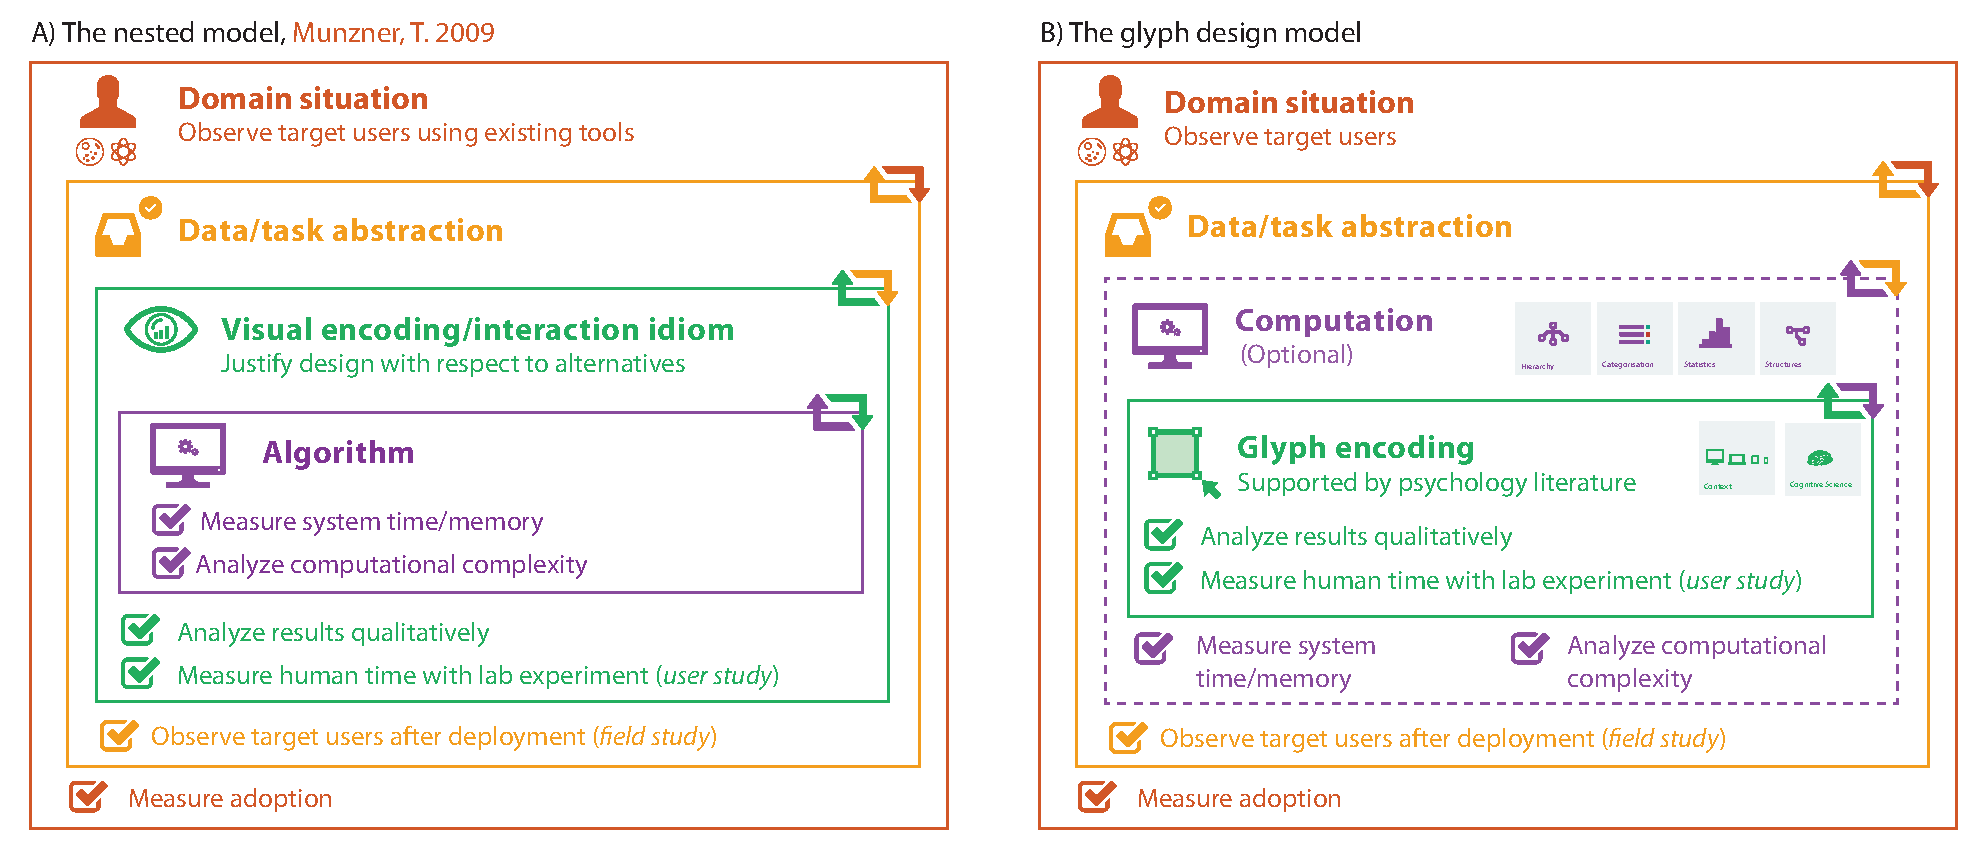
\includegraphics[width=\textwidth]{images/ch3/model}
%\caption{A) An overview of the ``nested model'' presented by Munzner \etal \cite{munzner2009nested}. B) A ``glyph design model'' inspired by the ``nested model''.}
%\label{fig:systematisation-models}
%\end{figure}

\begin{figure}[t!]
\centering
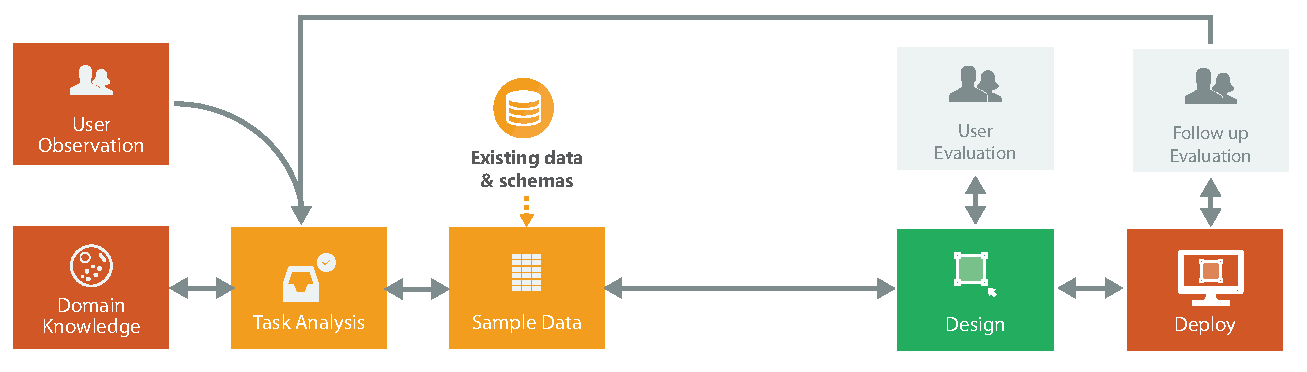
\includegraphics[width=\textwidth]{images/ch3/model_horizontal_simple}
\caption{A typical glyph design process modelled upon the ``nested model'' by Munzner \cite{munzner2009nested} where a designers instinct and iterations based on feedback from domain experts is core to the process.}
\label{fig:simple_process}
\end{figure}


Figure \ref{fig:simple_process} shows a typical representation of the glyph design process mapped to the components of the frequently followed ``nested model'' for visualization design by Munzner \cite{munzner2009nested}.
This model has the following components at its core:

\begin{itemize}
\item \textbf{User Observation} provides an opportunity to monitor users in their normal working environment.
Knowledge gained from this process can feed in to:
\begin{enumerate}
	\item \emph{task} definition through interviews and day to day observations of current working practices;
	\item \emph{design} processes via information about what a user is: willing to learn; willing to remember; and is able to remember. This ultimately affects the number of variables that can be encoded and how they are encoded. If a user has little time to remember glyphs, then they should be more accessible via increased use of metaphor for example; and 
	\item \emph{evaluation} to determine whether or not the solution meets user expectations and solves the problem the glyph was meant for.
\end{enumerate}

\item \textbf{Domain Knowledge} is of importance in any visualization since a good understanding of the domain will generally result in better visualizations that really solve the problems faced by the users.
Furthermore, domain knowledge carries additional importance in glyph-based visualization due to the common need for metaphor to support glyph learnability and memorability;

\item \textbf{Task Analysis} (or data/task abstraction in the ``nested model'') provides an indication of the types of visual queries that a user would like to make.
These tasks form the basis of data prioritisation.
For example, if a major task performed by a user was finding users of a particular age, making the age information more visually available is important;

\item \textbf{Sample Data} gives an indication of the data values (and ranges) to be encoded by the glyphs.
%These values can be processed by algorithms (see the \emph{computation} section) to find the most common values, the rarest values, and so forth depending on the visualization requirements.
A \emph{data representation schema} can provide additional information about the format of the sample data and the types of values  (\eg, categorical or quantitative) each field contains.
This in turn can be used in the design phase where design principles discussed below can be applied to ensure that appropriate visual channels are used for particular data values;

\item \textbf{Design} involves the selection of appropriate visual channels to represent each data variable to be encoded followed by the arrangement of those visual channels in 2D or 3D space;


\item \textbf{Evaluation} provides some level of validation that the glyph design is a success.
However, there are numerous ways in which a glyph may be evaluated.
They may be validated by reviewing the tasks defined earlier with users.
Glyphs could be evaluated in terms of their distinguishability, to ascertain whether or not users can detect differences between glyphs (if users cannot distinguish between glyphs, visual search will be impeded)?
If glyphs are providing an alternative to an existing visualization system, benchmarks on user accuracy and task speed can be made for comparison purposes.
If a glyph design does not perform effectively, there will be further iterations on the design to improve performance. 
When a design is approved, glyphs may be deployed in the day to day working environment of the domain experts.
Follow up studies can be conducted over time, and more iterations may be required.
\end{itemize}

Although this model represents the common visualization design practices, it does not offer direct solutions to help systematise glyph design.
Much of the details are still left up to individual designers to negotiate with domain experts.
In this way, the design process is referred to as \emph{ad hoc} (``for this'').
Due to a need for domain specific metaphor in glyph design, an \emph{ad omnia} (``for everything'') design process is unlikely to exist.
However, through incorporation of design principles, more objective decision making can be performed to control data to visual channel mappings for instance.
Additionally, computational techniques can present further opportunities to directly and indirectly (by proposing data features to be encoded) guide glyph design.

\begin{figure}[t!]
\centering
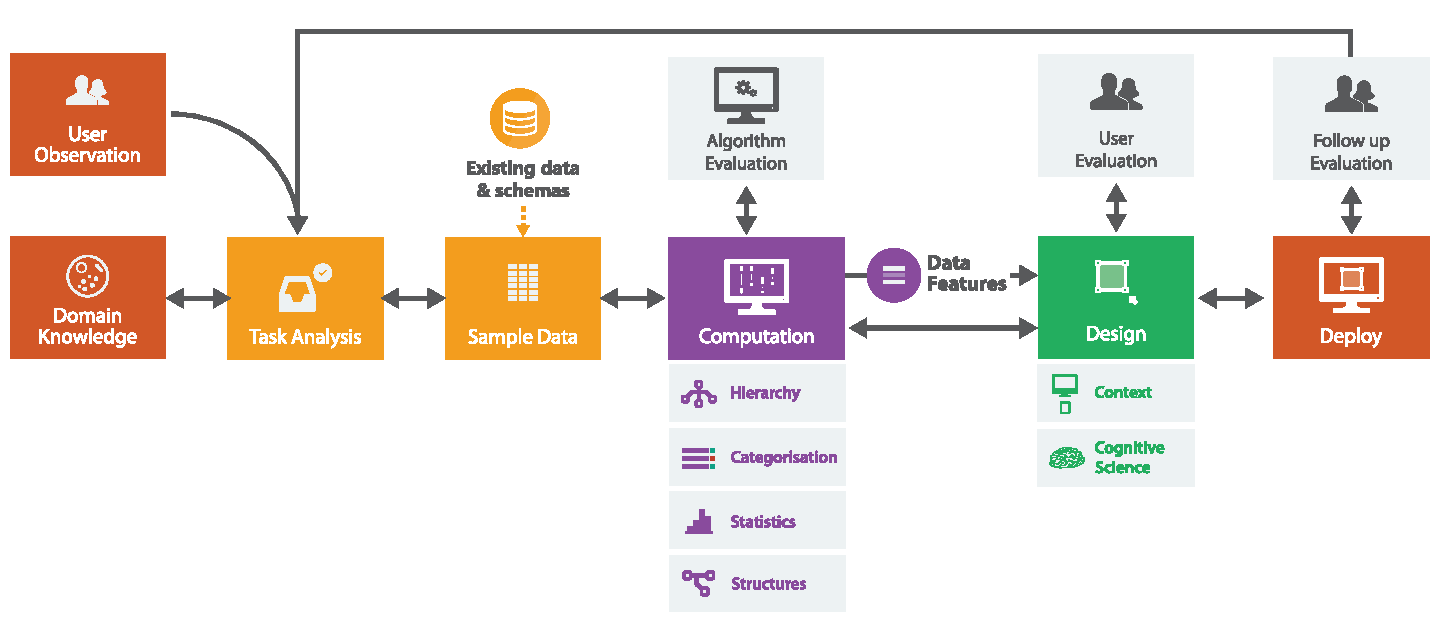
\includegraphics[width=\textwidth]{images/ch3/model_horizontal_new}
\caption{A more systematic approach to glyph design using computation to either directly inform the design step, or to provide data features to be used for glyph design. The design step is influenced by design principles and context.}
\label{fig:new_process}
\end{figure}

This chapter proposes an approach illustrated in Figure \ref{fig:new_process} for the systematic creation of glyphs.
Central to this approach is the addition of computational techniques to the model in Figure \ref{fig:simple_process}, and a more structured approach to the selection and arrangement of visual channels in the design step.
Our additions are there to reduce the reliance on subjectivity in the design process, however, staying true to the ``nested model'' \cite{munzner2009nested}, the importance of domain-expert interaction and evaluation is not downplayed.

The remainder of this chapter goes in to more detail on how these \emph{design} and \emph{computation} steps break down, and how individually and collectively they can contribute to more systematic and predictable glyph design.

\section{Design Principles}

\begin{figure}[t!]
\centering
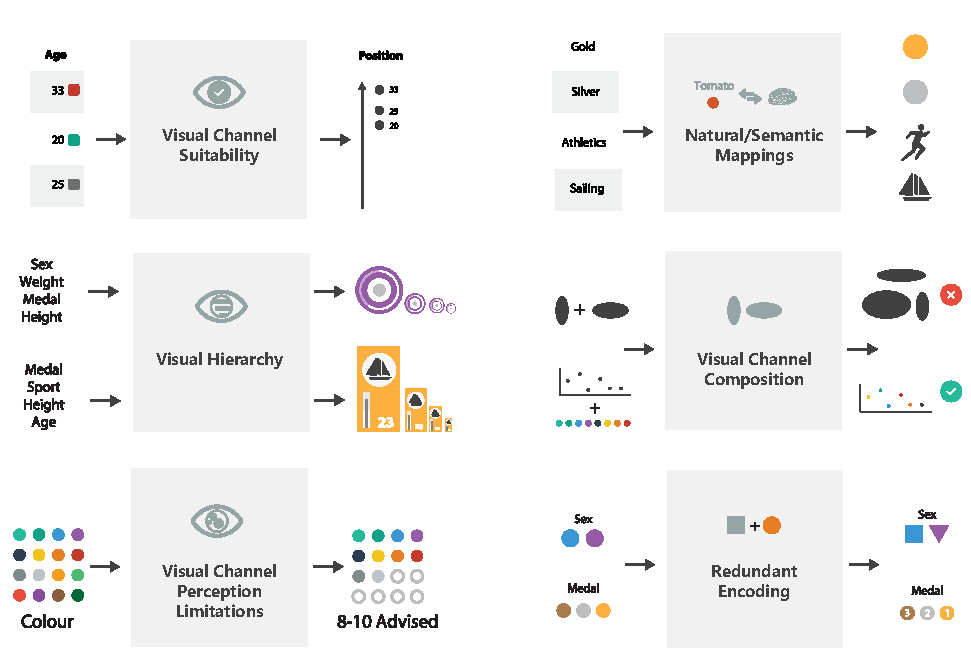
\includegraphics[width=\textwidth]{images/ch3/design_guidelines_2}
\caption{Design principles that can be followed to provide a more systematic approach to glyph design.}
\label{fig:strategies_design_guidelines}
\end{figure}

Ultimately, the goal of a systematic technique is to remove the level of randomness in some process.
For glyphs, the levels of randomness can be limited through integrating knowledge of how the visual system works in to the design process.
Core to such a process are a set of design principles based on research stated in Chapter \ref{chap:related_work} and illustrated in Figure \ref{fig:strategies_design_guidelines} consisting of:

\begin{enumerate}

\item \textbf{Visual channel suitability} in advises that data types within a glyph should be mapped to the correct visual channels.
This is based on work by Stevens \cite{stevens1975}, Bertin \cite{Bertin:1983:book}, Cleveland and McGill \cite{cleveland1984graphical}, Mackinlay \cite{mackinlay1986automating}, Heer and Bostock \cite{heer2010crowdsourcing};

\item \textbf{Natural mappings} suggests the use of semantically meaningful mappings of data to their natural visual counterparts where possible.
Using too many abstract colours or shapes for example would place a lot of cognitive load on a user to remember all mappings.
Make these colours or shape metaphoric however, and the glyph decoding process will be much easier, \eg, \textcolor{Red}{strawberry $\Leftrightarrow$ red}, \textcolor{Plum}{aubergine $\Leftrightarrow$ purple}, or \textcolor{Green}{money $\Leftrightarrow$ green} \cite{lin2013selecting}.
This principle is based work by Ware \cite{ware2010visual, ware13}, Borgo \etal \cite{Borgo12}, and Lin \etal \cite{lin2013selecting};

\item \textbf{Visual hierarchy} applies an organisation to the visual channels within a glyph given the importance of the data to some task.
This ensures that the most important classifiers of data are available even at the overview level of a visualization due to their visual prominence (visual hierarchy and global/local processing, and pre-attentive processing);

\item \textbf{Visual channel composition} suggests avoiding visual channels that are perceived holistically as opposed to separately.
The integrality or separability of a pair of visual channels is not a discrete decision.
While it is largely agreed that width and height are the most integral dimensions, while position and colour are the most separable, many other dimension lie on a continuum between fully integral and fully separable; 

\item \textbf{Visual channel perceptual limitations} provides guidance to avoid overuse of a visual channel such as colour whose perception degrades as the number of samples from each hue increases.
For example, distinguishing between four distinct colour hues is possible, but it is much harder to distinguish between sixteen distinct colours.
Colour maps like those provided in \emph{ColorBrewer} \cite{ColorBrewer} and \emph{Tableau} \cite{tableau_palettes} provide a good starting point for glyph designers; and

\item \textbf{Redundant encoding} suggests the use of multiple encodings for one data item so as to minimise the chance of error when reading glyphs in a display \cite{ware13}.
Redundant encoding may also speed up visual search.
For example, in Figure \ref{fig:strategies_design_guidelines} F, colour and shape are used to code gender.
Therefore, if the colour channel is impeded, shape can be used to distinguish between male and female glyphs.
\end{enumerate}

\section{Computation}

\begin{figure}[h!]
\centering
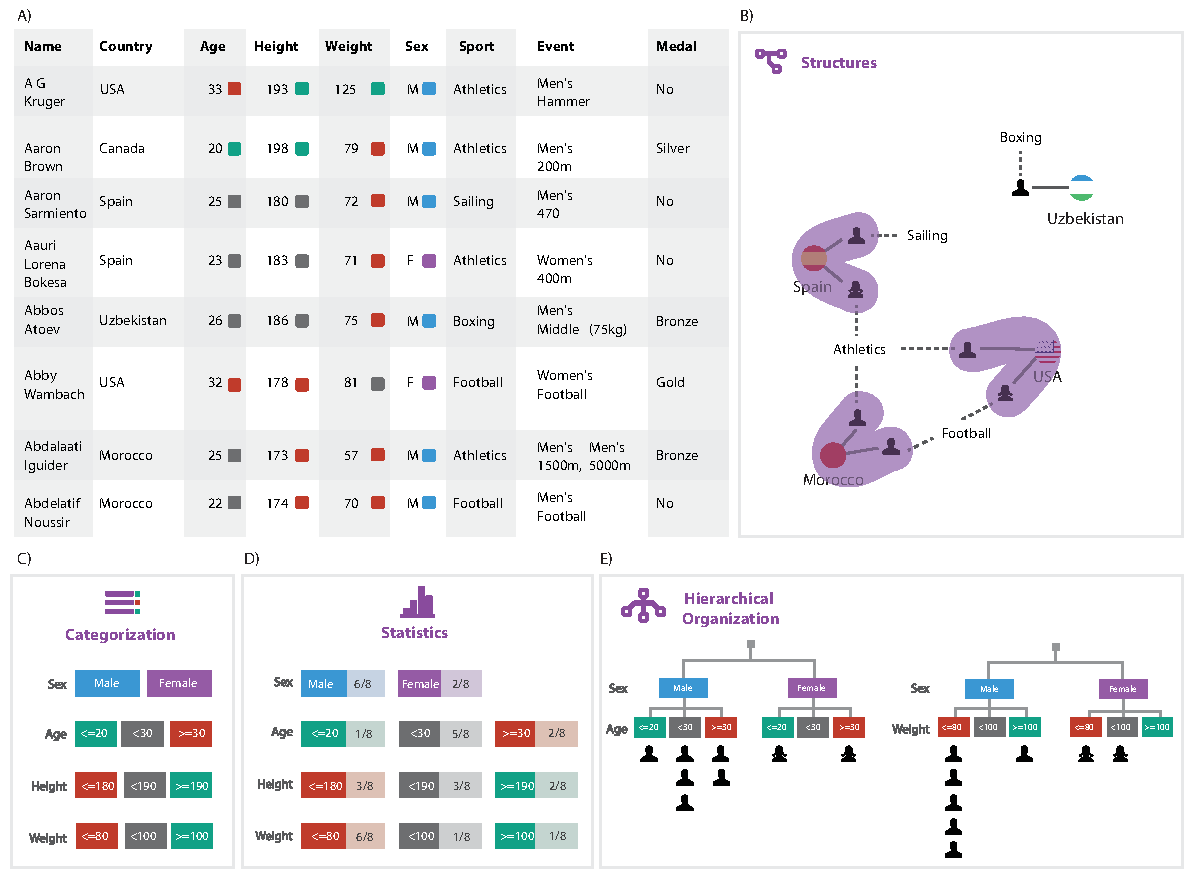
\includegraphics[width=\textwidth]{images/ch3/computation_benefits}
\caption{A) Table showing a subset of London 2012 Olympians with country, age, height, weight, sex, general sport, events, and if they won a medal.
B) By building a graph from the data from the table in A) certain structures can be mined in the data. Common structures in graphs or motifs could be a target for aggregation when the graph is very large.
C) We can create categories from the data that can be used directly to colour code ranges of values for instance.
D) Statistics can provide an indication of how balanced particular categories are, or what values are very common or very rare so that they may be highlighted or hidden depending on the user task.
E) Using categories from C) we can generate a tree/taxonomy that classifies the data in a structured way.
The choice of category will ultimately change the properties of the tree including how balanced it is (\eg, the tree on the left is more balanced than the one on the right since people are more evenly distributed at the leaf nodes).}
\label{fig:computational_benefits}
\end{figure}

Computation can be deployed to provide additional information about the data (derived data).
We have identified four techniques that can be applied either individually or combinatorially to help the glyph design process.
This influence may be direct, where the output of computation can be used to design glyphs.
Or it may be indirect, where computation identifies the features to be encoded using glyphs.
\begin{enumerate}

\item \textbf{Structure identification} (Figure \ref{fig:computational_benefits} B) generally refers to discovery of patterns in relational data, \eg, patterns in connectivity.
This information can be used to reduce complexity in network visualizations by removing common or uninteresting patterns, leaving behind the more important signals.
Figure \ref{fig:structure_compress_glyph} shows an example where we wish to find the common elements (motifs) in a graph and substitute these motifs with less complex glyph representations. 
Simple motif finding can be accomplished using an algorithm such as FANMOD \cite{wernicke06}.
This finds similar topologies in a graph and counts their occurrence.
The most common motifs are then put forward to be substituted in a simplified graph.

\begin{figure}[h!]
\centering
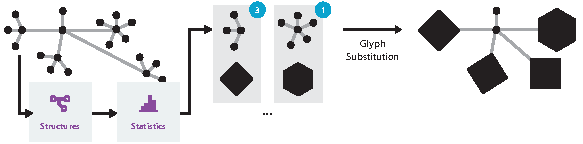
\includegraphics[width=\textwidth]{images/ch3/structure_compress_glyph}
\caption{Graph-based compression can make use of glyphs through the substitution of common structures/pattern/motifs with glyph alternatives.
This can be used to greatly reduce graph complexity as by Dunne \etal \cite{dunnemotif2012}.}
\label{fig:structure_compress_glyph}
\end{figure}

\item \textbf{Categorizations} (Figure \ref{fig:computational_benefits} C) provide a way of splitting the data based on various categorisations.
For example, in Figure \ref{fig:computational_benefits} C, there are four classifications schemes for sex, age, height and weight.
Each of these schemes has a number of ``classes'', and the data is likely to be distributed differently across those different categories.
These schemes could be determined computationally using algorithms such as k-means \cite{macqueen1967} or hierarchical-based (\eg, \cite{Sibson01011973}) clustering.
However these approaches are often inaccurate and computationally expensive.
Another approach is to use a more supervised approach to clustering with the aid of computation, a large representative data set, and domain experts in the loop to ensure that categorisations are meaningful and not too granular.

Such categorisations, when computed can be used to group data records based on a range of values, rather than singletons.
For example, in Figure \ref{fig:computational_benefits} C athletes can be grouped by their age, height, or weight range.
What this means in terms of glyph design is that instead of representing every possible age, height, or weight, we can represent just three ranges showing the normal and two outlier ranges.
Going back to Chapter \ref{chap:related_work}, this has implications for improved visual search, since now to find a class of value, a user need only search for one of three values.
Comparing between three sizes, colours, or shapes is much easier than between ten or more.

\item \textbf{Statistics} (Figure \ref{fig:computational_benefits} D) is generally helpful since it can provide information about the distribution of data, this can feed in to the categorisation process for example.
Statistical processes can also help identify the common/rare data features to be encoded using glyphs to bring attention to such features in a visualization.

\begin{figure}[t!]
\centering
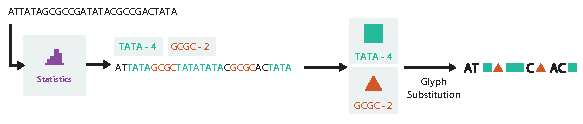
\includegraphics[width=\textwidth]{images/ch3/statistics_compression}
\caption{Text-based compression can use glyphs to replace common text with visual representations.
In this case, some common DNA motifs are replaced with coloured shapes.
Since reading text is a cognitively demanding process, showing structures of interest visually can speed up interpretation.
}
\label{fig:text_compress_glyph}
\end{figure}

For example, in Figure \ref{fig:text_compress_glyph} statistical processes are used to find the most common four letter sequences in a string representing a small region of DNA.
By finding the common elements and replacing them with coloured shapes, the \textcolor{Green}{TATA} and \textcolor{red}{GCGC} regions can be found more easily in the DNA sequence using glyphs rather than text.
This technique takes advantage of the supposed iconic memory identified by Sperling \cite{sperling60}.

\item \textbf{Hierarchical Organization} (Figure \ref{fig:computational_benefits} E) refers to the creation of a taxonomy, a tree representation that hierarchically defines the properties of items (leaf nodes) in the tree.
Maguire illustrated many examples of taxonomies in biology and visualization \cite{maguire12} including the tree of life in biology that categorises all species by their Kingdom --> Phylum --> Class --> Order --> Family --> Genus --> Species. 
For glyph design this hierarchical organisation can be used to structure how a glyph is arranged.
Imposing an order to the design should facilitate better learnability and memorability of the resulting glyphs since the formation of each glyph should follow a rule.

\begin{figure}[h!]
\centering
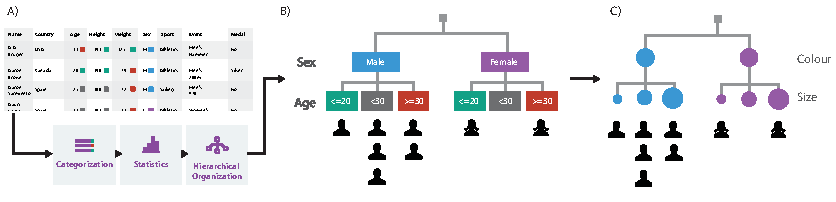
\includegraphics[width=\textwidth]{images/ch3/table_tax_glyph}
\caption{A) Starting with our table of Olympians, categorize the data, perform the statistical analysis, and generate the hierarchical organization.
B) The result of the hierarchical organization process is a taxonomic tree that represents the original data in a structured way.
C) From the hierarchical results, a glyph can be designed by assigning a visual channel to each level in the taxonomic tree where the visual channel assigned is decided by data type, and the ``strength'' of the visual channel.}
\label{fig:taxonomic_glyph_design}
\end{figure}

Figure \ref{fig:taxonomic_glyph_design} shows how one may traverse from a collection of records in a table to a taxonomic tree, then a glyph based representation of people within that tree by sex and age categories.

\end{enumerate}

\section{Summary}

So far, we have presented a hypothesis on how glyph design could be made better, and outlined a ``model'' in Figure \ref{fig:new_process} that could be followed to test this hypothesis.
The remainder of this thesis will apply this model to a number of scenarios and investigate how design principles and computation can contribute to a more systematic glyph design.

All further chapters apply different mixtures of design strategies by using flavours of the model defined here where computation and evaluation techniques in particular will vary.
Listed below is a summary of the work conducted in this thesis and the strategies used in relation to our systematic framework shown in Figure \ref{fig:strategies_examples}

\begin{figure}[b!]
\centering
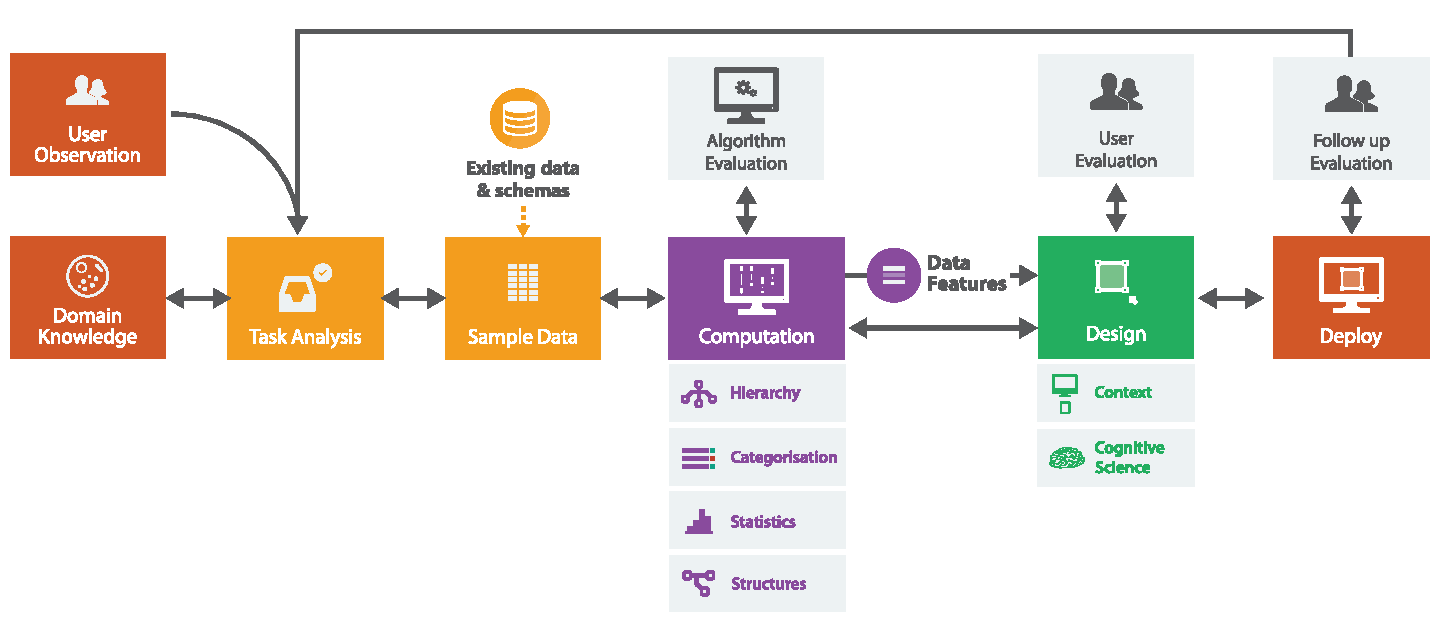
\includegraphics[width=\textwidth]{images/ch3/model_horizontal_new}
\caption{Our framework for more systematic glyph creation.}
\label{fig:strategies_examples}
\end{figure}


\begin{enumerate}

\item \textbf{Chapter \ref{chap:glyph-tax}}:
\begin{itemize}
\item \emph{Users:} Biologists (domain experts involved in work).
\item \emph{Sample Data:} ArrayExpress \cite{ArrayExpress::2012} repository with over 1.2 million individual experiments.
\item \emph{Computation:} Categorisation, statistical analysis, and hierarchical organisation of biological sample characteristics (\eg, organism, organism parts) and processes.
\item \emph{Design:} Uses the computationally generated taxonomy in combination with visual channel orderings and design principles.
\item \emph{Evaluation:} Domain expert evaluation (two biologists and trained data curators from the University of Oxford).
\item \emph{Deployment:} Used in a popular data annotation and curation tool called ISAcreator \cite{rocca-serra10}.
\end{itemize}

\item \textbf{Chapter \ref{chap:automacron}}:
\begin{itemize}
\item \emph{Users:} Biologists (domain experts involved in work).
\item \emph{Sample Data:} ArrayExpress \cite{ArrayExpress::2012} repository with over 1.2 million biological experiments.
\item \emph{Computation:} Structure analysis of biological workflow graphs from Chapter \ref{chap:glyph-tax}, and statistical analysis.
\item \emph{Design:} Uses the motif finding algorithm to automatically generate multi-resolution glyphs by following design principles.
\item \emph{Evaluation:} Motif finding algorithm performance comparison and domain expert evaluation (two biologists and trained data curators from the University of Oxford).
\item \emph{Deployment:} Available as a standalone tool for error detection tasks, and to build macro glyph libraries.
Also used in the ISAcreator \cite{rocca-serra10} tool to compress common patterns in biological workflows.
\end{itemize}

\item \textbf{Chapter \ref{chap:timeseries}}:
\begin{itemize}
\item \emph{Users:} Zoologists and statisticians (Oxford University), and analysts at an online betting company.
\item \emph{Sample Data:} Space shuttle and electrocardiogram data from Keogh \etal \cite{shuttle_data} .
\item \emph{Computation:} Statistical analysis to identify common time series patterns and count their occurrence.
\item \emph{Design:} Uses design principles to drive the glyph creation process.
\item \emph{Evaluation:} Baseline comparison with ground truth anomalies. Users from industry (online casino), and zoologists from the University of Oxford tested the interface and algorithm results.
\item \emph{Deployment:} General purpose web application.
\end{itemize}

\item \textbf{Chapter \ref{chap:processes}} introduces a number of additional examples showing how the systematicism introduced in this thesis can be applied to areas such as biological sequence analysis, poetry, and security analysis.
These examples also use different evaluation approaches, and the last example introduces a method to perform some quantitive evaluation on glyphs.
\begin{enumerate}
\item Biological sequence visualization:
\begin{itemize}
\item \emph{Users:} Biologists/Bioinformaticians.
\item \emph{Sample Data:} DNA sequences for the same region in 1809 bacteria.
\item \emph{Computation:} None.
\item \emph{Design:} design principles followed to drive the glyph creation process.
\item \emph{Evaluation:} A domain expert (Dr. Philippe Rocca-Serra, a biologist from the University of Oxford) was involved in the design process throughout, followed by an online user survey with forty-two biologists and bioinformaticians.
\item \emph{Deployment:} Open-source sequence logo library viewer for the web.
\end{itemize}

\item Poetry visualization:
\begin{enumerate}
\item \emph{Poetry glyph}:
\begin{itemize}
\item \emph{Users:} Humanities scholars (poets).
\item \emph{Sample Data:} Numerous poetry, English texts and scientific literature.
\item \emph{Computation:} None.
\item \emph{Design:} design principles followed to drive the glyph creation process.
\item \emph{Evaluation:} Two poets (from the University of Utah), and a language scholar (from the University of Oxford) were involved in the design process.
The same experts evaluated the resulting software tool.
\item \emph{Deployment:} An online tool called PoemViewer \cite{CGF:Abd2013a}.
\end{itemize}
\item \emph{Macro glyph}:
\begin{itemize}
\item \emph{Users:} Humanities scholars (poets).
\item \emph{Sample Data:} Numerous poetry, English texts and scientific literature.
\item \emph{Computation:} Statistical and structural analysis.
\item \emph{Design:} design principles followed to drive the glyph creation process.
\item \emph{Evaluation:} Semi-structured interviews with three English DPhil students, and an English professor from the University of Oxford.
\item \emph{Deployment:} An online tool called PoemViewer \cite{CGF:Abd2013a}.

\end{itemize}
\end{enumerate}

\item File system event visualization:
\begin{itemize}
\item \emph{Users:} Security analysts for file system monitoring.
\item \emph{Sample Data:} Dropbox and Git log data.
\item \emph{Computation:} None.
\item \emph{Design:} Uses a new technique called the quasi-Hamming distance to create visually separable glyph designs that support error detection and correction.
\item \emph{Evaluation:} Computer- and user-based glyph similarity metrics for glyph designs.
\item \emph{Deployment:} Available in a file system visualization library called TreeLines. Deployed in a monitoring environment for a cybersecurity research application.
\end{itemize}
\end{enumerate}


\end{enumerate}
\chapter{Taxonomy-Based Glyph Design---with a Case Study on Visualizing Workflows of Biological Experiments}


%% Uncomment below to include a teaser figure.
%  \teaser{
%  \centering
% \includegraphics[scale=.295]{images/glyph-taxonomy/bio-workflow-isacreator.eps}
% \caption{a) Workflow as rendered currently using toolkits such as GraphViz. b) We propose to replace the textual labels with glyphs, while allowing interactive access to detailed descriptions. This makes it easy to gain an overview, search components and compare workflows. The screenshot shows a prototype developed within ISAcreator, a system for capturing biological experiment metadata.}
% \label{fig:teaser}
%  }


%% Uncomment below to disable the manuscript note
%%\renewcommand{\manuscriptnotetxt}{}

%% Copyright space is enabled by default as required by guidelines.
%% It is disabled by the 'review' option or via the following command:
% \nocopyrightspace

%%%%%%%%%%%%%%%%%%%%%%%%%%%%%%%%%%%%%%%%%%% %%%%%%%%%%%%%%%%%%%%%
%%%%%%%%%%%%%%%%%%%%%% START OF THE PAPER %%%%%%%%%%%%%%%%%%%%%%


%% The ``\maketitle'' command must be the first command after the
%% ``\begin{document}'' command. It prepares and prints the title block.

%% the only exception to this rule is the \firstsection comman

\section{Introduction}
\label{sec:Introduction}
\emph{Glyph-based visualization} is a class of visual representations where a collection of small visual objects (referred to as \emph{glyphs}) are used to encode different attribute dimensions of an input data space.
A good glyph design can enable users to conduct visual search more efficiently during interactive visualization, and facilitate effective learning, memorizing and using the visual encoding scheme.
A less effective visual design may suffer from various shortcomings such as being perceptually confusing, semantically ambiguous, difficult to learn and remember, or unable to accommodate low-resolution display devices.
Most accepted designs have undergone an enduring process of evolution, refinement and standardization.
One could not and should not remove the necessity for such processes in glyph design.
Meanwhile, the design process for a glyph set usually relies on an assortment of creativity, artistic skill, domain knowledge, intuition about users, and sometimes personal preference.
While most of these qualities are absolutely helpful and some are inevitable, it is highly desirable to introduce ``systematicism'' and objectivity into the design process.

To demonstrate our approach, we elected the field of experimental biology as a test bed for developing a systematic methodology to create a glyph-based visual mapping for visualizing experimental design and experimental processes. While experimental design is at the heart of biological data evidence gathering, representation of such information is confined to either verbose description or ineffective representations. This claim is backed by a survey of public biodata repositories, devised to ensure data perennity, scientific scrutiny and reproducibility. As illustrated in Fig. \ref{fig:teaser}(a), workflows are traditionally drawn as text-based diagrams. Text labels are indices of concepts, and usually they do not encode multivariate information directly. Text-labeled boxes are costly in terms of display space usage as well as time required for visual search since parsing and interpretation of text is a slow post-attentive process \cite{ware04}. They are particularly ineffective when one needs to compare between different workflows or to identify unusual or missing components in a workflow.

Therefore, exploring an alternative in the form of glyph based representations, which are at the core of many successful schematic diagrams in the history of sciences, engineering and business management, offers a potentially more effective means for depicting these workflows.  
This presents us with an interesting case study where other types of design approaches would not be appropriate, especially in dealing with several hundreds of conceptual names.

It is important to note that domain experts are in general more willing and able to learn and memorize an encoding scheme in order to improve the accuracy and efficiency of routine tasks. At the same time, it is also necessary for an encoding scheme to facilitate effective learning and remembering through appropriate abstraction and metaphors.

Motivated by this case study, we made an observation that when a large number of concepts (or taxa) are organized into a taxonomic tree, the hierarchy typically represents an ordering of different categorization schemes.
The schemes that are higher-up in the taxonomy (closer to the root) are usually considered to be more important, which reflect their conceptual coverage, frequency of usage, domain-specific convention, and some other measurable factors.
In terms of visual encoding, higher up schemes should ideally be mapped to visual channels that have more discriminative capacity.
Hence, we can explore the parallel between the taxonomic hierarchy and the ordering of visual channels based on discriminative capacity to formulate a systematic and relatively objective process for designing a glyph set. This approach addresses one of the most common criticisms of data glyphs: the data to visual attribute mapping bias \cite{ward08}. 
Given a large data repository that encompasses many concepts, our design process is composed of four major steps:
(i) gathering and processing raw metadata for obtaining a set of taxa (names);
(ii) formulating a taxonomy based on a set of categorization schemes (Section \ref{sec:Taxonomy});
(iii) carrying out visual design, which includes the sub-process of determining the ordering of visual channels, proposing optional visual mappings, and identifying metaphoric abstractions and associations (Section \ref{sec:Glyphs}); and
(iv) implementing a glyph-based visualization system, in our case, for depicting workflows of biological experiments (Section \ref{sec:Workflow}).

Similar to most design processes, it is helpful to conduct all stages in a progressive and iterative manner.
As glyph-based visualization is normally deployed in a specific application domain, it is important to involve domain experts at every stage of the design process.
During this work, we met with domain specialists on a weekly basis.

\section{Related Work}
\label{sec:RelatedWork}
In this section, we give a brief overview of two most relevant areas in visualization, \emph{glyph-based visualization} and \emph{workflow visualization}.
The remainder background information includes the biological data management, perceptual guidance, and categorization algorithms, which will be described in the following sections where the relevant technical details are discussed.

\subsection{Glyph-based Visualization}
%
There are many examples of glyph usage in the literature spanning many disciplines, especially in conjunction with many schematic diagrams.
Bertin considered a range of simple glyphs in the context of geo-information visualization \cite{bertin83}.
Ward surveyed the use of glyphs in visualization, and discussed a number of bias issues, design approaches, and layout options \cite{ward08}.
Ropinksi \emph{et al.} conducted a survey on glyph-based techniques in medical visualizations \cite{ropinski11}.
In visualization, a number of interesting glyph designs have been presented with noticeable impact on a large range of applications (e.g., 
medicine \cite{Kindlmann06},
software \cite{Chuah98},
text \cite{Rohrer98}, and
scientific computation \cite{Wittenbrink96}).
Furthermore, Ribarsky \emph{et al.} developed an editing system, Glyphmaker \cite{ribarsky94}, to assist the process of designing glyphs.
Post \emph{et al.} proposed a language, Icon Modeling Language, for creating glyphs and glyph-style contours \cite{post95}.

There have been some recent efforts to use glyph-based visualization in biological sciences.
One noticeable attempt is the \emph{Systems Biology Graphical Notation} (SBGN) \cite{lenovere09}.
The design of SBGN makes use of the notional representations of UML with some modifications to describe the biological entities and their interactions within a biological system.
GenoCAD \cite{cai10} provides a grammar-based language for representing and searching DNA sequences and for building genetic constructs from DNA sequences, facilitating the use of conventional link diagrams.
Both systems rely heavily on text labels.
In handling a large collection of workflows, they exhibit a few shortcomings, such as inefficiency in using display space and ineffectiveness in supporting some visualization tasks, such as comparisons and novelty or anomalies detection in workflows.

In the literature, several authors encouraged glyph designers to consider visual perception when constructing glyphs \cite{ward08,karve07}. Others examined the design space of icons, which normally encode less information than glyphs (e.g., \cite{hemenway82,lewis04}). There were perceptual studies showing the merits of icons over text labels (e.g., \cite{muter86,pellegrino77}), as well as those showing the contrary (e.g., \cite{wiedenbeck99}).
Building on such discussions, this work aims to address a methodological need for a systematic approach to glyph design for applications where large collections of concepts need to be visually encoded using glyphs.

%%In \cite{ward08}, Ward summarizes that there is a need for novel mechanisms to display the growing amounts of information becoming available via the data deluge. He details the need for multi-resolution strategies \cite{ward08} giving varying levels of detail proportional to a users focus on the overall visualization.%%

\subsection{Workflow Visualization}
%
The need for \emph{workflow visualization} is pervasive across many different domains.
For example, in business and management the Gantt chart is a form of text based workflow visualization, while BPMN (Business Process Model and Notation) and EPC (Event-driven Process Chain) make use of icons to enrich text labels.
In engineering disciplines, various schematic diagrams, such as UML (Unified Modeling Language), Petri-net and circuit diagrams, are used to convey data flow and process interaction.

In this work, we consider workflows used to describe biological experiments. 
This class of workflow visualization renders the processes enacted on biological materials in an experiment (e.g., removal of blood sample from patient).
There has been little effort to develop tools that address the domain-specific needs.
Scientists usually use generic text-based graph drawing tools such as GraphViz \cite{graphviz}.

One related aspect is \emph{pathway visualization}, which is concerned with the rendering of cellular biological processes. An array of pathway visualization tools have been developed, some of which incorporate glyphs.
For example, VANTED \cite{junker06} overlays glyphs representing gene expression, enzyme and metabolite profile data on top of pathway diagrams from KEGG \cite{ogata99}.
GENeVis \cite{bourqui09}, which also employs glyphs to represent multivariate data, is a comprehensive visualization toolkit for exploration of pathways in conjunction with temporal data.
GenoCAD has at its core a workflow generation system and relies on their glyph library for rendering of the different biological processes within a cell.
SBGN-ED \cite{czauderna10}, is an add-on for the VANTED software and performs pathway creation using the aforementioned SBGN \cite{lenovere09} visual language.

%Analysis of biological data is typically a multi-stage process, involving multiple data types and sources, manipulations and algorithms.
%Graph drawing tools have been made available for bioinformaticians to keep track of these processes and to make the analysis process reproducible and sharable.
%For example, Taverna \cite{missier10} exploits color-coded boxes combined with text to indicate process type.
%KNIME \cite{berthold08} uses glyphs to indicate process types in combination with more detailed text descriptions.


%%Pathline\cite{meyer10}, a tool to visualize gene expression alongside metabolite information within particular biological pathways; 

% ====================
\section{Motivation and Overview}
\label{sec:Motivation}
%
The advent of massively parallel techniques such as DNA microarray, mass-spectrometry based proteomics and metabolomics and next generation sequencing enables molecular biologists to collect, process and manipulate biological signals on a new scale.
Big data in biology is a reality.
There has been serious effort in biology to ensure quality of experimental records by providing data archiving infrastructure and defining standards for adequate annotation and sufficient details for recapitulation of results.
A number of molecular biology signature databases have been or are being established to cover the main molecular dimensions: transcript, protein and metabolites.
The captured metadata mostly revolves around a similar configuration where sets of samples corresponding to different conditions are processed, measurements produced and analysis performed, delivering data that needs to be handled and interpreted.
While the availability of such metadata facilitates comparison across datasets and enables meta-analysis, providing means to serve an overview of experimental design can assist analysts and data managers alike, from data selection according to relevancy, to error detection such as imbalances, irregularities or inconsistencies in records.

\textbf{Task Analysis.} In the context of meta-databases for experimental records, there are two main groups of users. The majority of users are those who create data for their biological experiments or retrieve data relevant to their scientific interests. Their tasks include:
(a) entering and editing their own experimental records;
(b) transforming workflow records to schematic diagrams for comparison, external memorization, publication and education;
(c) uploading and downloading datasets;
(d) querying and searching for relevant experiments;
(e) understanding workflows of existing experimental designs;
(f) identifying similarity and difference between workflows for a common task;
(g) understand pooling events and sample relations (derivation).

The second group of users are curators who manage data archives. As biology or bioinformatics scientists themselves, they perform the above-mentioned tasks (d)-(g) frequently, and (b)-(c) occasionally. In addition, they also carry tasks for:
(h) checking syntactic correctness of submitted workflows;
(i) checking semantic correctness of submitted workflows which usually involves reading the associated publications then comparing the submitted workflows with those described in the publications;
(j) interacting with authors of submitted workflows to clarify any inconsistency and misunderstanding;
(k) making appropriate corrections in submitted records where necessary;
(l) augmenting with appropriate annotation based on additional information found in the associated publications;
(m) providing authors with submission feedback.
(n) forming an up-to-date overview about the experiments in the data archives, and maintaining an insight about the provenance of the archives;
(n) analyzing the grouping, replication, distribution and trend of experiments;
(o) analyzing ambiguities, errors and uncertainty in experimental recording, and identifying the need to enrich and refine the relevant standards for ontology, labelling and annotation.
(p) providing tools to assist users in creating meta-data from raw data.

It is not difficult to observe that effective workflow visualization can significantly improve users' capability in performing tasks b, e, f, g, h, i, j, l, n, o and p.

While it is necessary to evolve a glyph-based design for workflow visualization over a period, it is also important not to make the first step in an ad hoc manner. Such a process does not scale well with the requirements of the application concerned where a large
number of concepts are to be encoded using glyphs. We thus adopt a new systematic process for glyph design by exploring the parallel between the hierarchy of concept categorization and the ordering of discriminative capacity of visual channels. Fig. \ref{fig:workflow} depicts this process.

\begin{figure}[t!]
\centering
\includegraphics[scale=0.56]{images/glyph-taxonomy/workflow.eps}
\caption{A systematic process for creating glyph based representations.}
\label{fig:workflow}
\vspace{-10pt}
\end{figure}

\textbf{Data Capture and Processing}. We first retrieved workflow metadata from a biological repository (content of the ArrayExpress archive), through use of a multi-threaded harvesting operation. All experimental workflows were then converted using a MAGE-Tab to ISA-Tab converter, the latter format being more general than the former and can be used to carry metadata payloads for many types of experiments, making the data processing program more ``future-proof''.

From the 21,000 ISA-Tab files, we extracted all names of protocols (processes) and biological materials, chemical materials, devices and data used in annotation. We also computed the occurrence of each material and process found in the entire set of ISA-Tab files, which have been used as one of the metrics in the next stage (see Section 5 for details). This step results in 61 process names and 3492 names of inputs and outputs (e.g., biological and chemical materials, device measurements and data).

\textbf{Taxonomy Formulation}. Since a taxonomy for such a large collection of terms is absent, we, for starters, established a set of categorization schemes with the help of domain experts. For example, one of the schemes for categorizing processes may be based on different biological inputs to a process (e.g., molecule, cell, organism, etc.). Another scheme may be based on processing methods (e.g., perturbation, combination, etc.). We computed the quality measures of each scheme based a set of generic metrics (see Section \ref{sec:Taxonomy}) then created a taxonomic tree by recursively selecting the best categorization scheme based on the quality measures. We finalized the organization of the taxonomy by allowing domain experts (2 co-authors) to make adjustments according to domain-specific conventions. All leaf nodes of the resulting taxonomy tree are names extracted from the workflow metadata. All non-leaf nodes represent a categorization scheme.

\textbf{Glyph Design}. First, we established an ordering of commonly-used visual channels based on the literature focused on perception and visualization (see Section \ref{sec:Glyphs}). This allows us to systematically compare the order of categorization schemes in the taxonomy with the order of different visual channels. Ideally, schemes at the upper level of the tree can be mapped to visual channels which are more prominent to our visual system.

We then proceeded to the glyph design process involving two intertwined sub-processes for \textbf{visual mapping} and \textbf{metaphoric abstraction and association}. We proposed various options of visual channels for each categorization scheme featured in the taxonomic tree. We considered the merits of these visual channels and identify potential conflicts with the visual channels that have been assigned to other schemes. With the direct help from domain experts, we tried to identify a metaphoric abstraction
or association for each design option proposed. We evaluated and recorded the intuitiveness and suitability of the abstraction and metaphor association.

Informed by the results the two sub-processes, we finalized a glyph set by selecting a design option for each scheme, while maintaining the order of discriminative capacity of visual channels, minimizing conflicts between different channels, and maximizing the use of metaphoric abstraction and association.

\textbf{Implementation of Glyph-based Visualization}. We then integrated the glyph set with a layout algorithm to form a prototype system for workflow visualization (see Section \ref{sec:Workflow}). For demonstration purposes, we tested the workflow visualization in conjunction with ISAcreator, a popular domain agnostic biological experiment metadata capture tool.

% ==================
\section{Taxonomy Generation}
\label{sec:Taxonomy}

Given a large collection of concepts, we should ideally make use of a standard taxonomy, where non-leaf nodes represent different categorization schemes and each scheme provides subclasses that lead to different sub-trees. In many circumstances, however, there is no agreed taxonomic tree as establishing a standard categorization requires non-trivial scientific effort that often spans over a few decades.

The algorithm described below is not intended to establish a semantic-rich taxonomic tree for classifying concepts.
It is designed purely for addressing the needs for ordering various categorization schemes (when there is no such an agreed order) to aid glyph design, and for devising a useful tree data structure in implementing the mapping between concepts and glyphs in workflow visualization.

Hence, the criteria used for structuring the tree are based on usage of the concepts and the structural quality of the tree to be constructed.

Taxonomy is a long standing concept that can be traced back to 3000BC \cite{maguire12}. Automatic taxonomy generation has been an active field in computer science and computational biology with existing work largely focusing on clustering algorithms (e.g., \cite{krishnapuram03}). Many such algorithms assume the availability of similarity measures for ordering entities rather than relying on the existence of individual categorization schemes. In these algorithms, there is usually no attempt towards application of a metric for creating meaningful non-leaf nodes in the resulting tree. In this work, it is essential to keep each categorization scheme as a non-leaf node unless it is redundant.

\subsection{Ordering Classification Schemes}
\label{sec:Algorithm}

Let $\mathcal{X} = \{ x_{1}, x_{2}, \ldots, x_{n} \}$ be a set of concepts to be classified.
In our application, this is the set of all valid names of biological processes and IOs (inputs and outputs) in the database.
Each concept $x_i$ is associated with a scalar value, $\mu_i \in [0, 1]$, indicating its frequency of usage in relation to the total occurrence of all concepts in the database.
There are a number of categorization schemes, $\mathcal{S} = \{ S_1, S_2, \ldots, S_m \}$.
Each scheme, $S_k$ divides concepts into several classes, $c^k_1, c^k_2, \ldots, c^k_{l_k}$.
The relationship between the concept set $\mathcal{X}$ and different classification schemes can thus be represented by a Boolean matrix, $\mathbf{A}$, where each element $\alpha[i,j,k] = 1$ if concept $x_i$ belongs to the $j^{th}$ class of scheme $S_k$; otherwise $\alpha[i,j,k] = 0$.
In the context of feature-based categorization, one can also view each scheme $S_k$ as a feature, and each class under $S_k$ as a particular type of this feature.
Without losing generality, we assume that the classes under the same $S_k$ are disjoint.
It is also possible that a concept does not possess the $k^{th}$ feature, and hence does not belong to any class under $S_k$.

Given the above categorical information about the concept set $\mathcal{X}$, one can choose a categorization scheme $S_k \in \mathcal{S}$, which will divide $\mathcal{X}$ into a number of disjoint subsets corresponding to classes $c^k_1, c^k_2, \ldots, c^k_{l_k}$ and $c^k_0$.
The subset $c^k_0$ contains those concepts which $S_k$ is unable to classify.
The partitioning process can be repeated recursively by applying one of the remaining categorization schemes in $\mathcal{S}$ to each subset.
This results in a hierarchical categorization tree, which defines a taxonomy for the concepts set $\mathcal{X}$.

The ordering of the schemes in $\mathcal{S}$ thus determines the taxonomic structure of $\mathcal{X}$.
It is not difficult to anticipate that many criteria can be used to determine the ordering for a given concept set.
Some criteria will no doubt encode application-specific semantics, and some may be subjective or debatable.
However, there are also some common-sense criteria that are generic to most applications.
These include:

\textbf{Coverage}.
The number of concepts that can be classified by scheme $S_k$ is a capacity measure of $S_k$.
The more concepts that $S_k$ can classify (i.e., the fewer in $c^k_0$), the better.
The measure, which is normalized by the set size $\mid\!\mathcal{X}\!\!\mid=n$, can be defined as:

\begin{equation}
\label{eq:Coverage}
  M_1(S_k) = \frac{\sum_{i=1}^{n} \max_{1 \leq j \leq l_k} (\alpha_{i,j,k})}{n}.
\end {equation}

\textbf{Potential Usage}.
A categorization scheme that is higher up in the taxonomical tree is expected to be used more often in the application concerned.
The occurrence frequencies of concepts, $\mu_i$, enable us to estimate the potential usage of a classification scheme as follows:

\begin{equation}
\label{eq:Usage}
  M_2(S_k) = \frac{\sum_{i=1}^n \mu_i \max_{1 \leq j \leq l_k} (\alpha[i,j,k]) }
  {\sum_{i=1}^n \mu_i}.
\end {equation}

\textbf{Subtree Balance}.
Having a balanced node distribution in a tree is a desirable property of a tree structure.
It prevents a tree from having an excessive height, which corresponds to the need for more visual channels.
Let $l_k$ denote the number of subclasses in categorization scheme $S_k$,
$\tau_j$ be the number of concepts in each subclass $c^k_j, j=1, 2, \ldots, l_k$ and $\sigma_{\tau}$ and $\bar\tau$ be the standard deviation and mean respectively of $\tau_1, \ldots, \tau_{l_k}$.
We can measure the level of balance as follows:

\begin{equation}
\label{eq:Branch}
  M_3(S_k) = \begin{cases}
    0 & \sum_{i=1}^{l_{k}} \tau_{l_i} = 0 \\
    1 & \sigma_{\tau} < \epsilon (\epsilon \gt 0) \\
    P(\bar\tau \pm1 \mid N_{\bar\tau, \sigma_{\tau}}) & \bar\tau \gt 0 \; \& \;\sigma_{\tau} > \epsilon
  \end{cases}
\end {equation}

\noindent where $P$ is the probability that a value within $[\bar{\tau}-1, \bar{\tau}+1]$ falls under
the curve given by the normal distribution $N$ with $(\bar{\tau}, \sigma_\tau)$ \cite{patel96}.
There are two special cases.
When all values of $\tau_j$ are 0, $S_k$ cannot classify any concept; hence the metric returns a zero score.
When $\sigma_\tau = 0$, the subtree is totally balanced; hence the metric returns one.
As $\sigma_\tau$ approaches zero, the function $P$ becomes numerically unstable, we use a cut-off value $\epsilon$ to prevent this. In this work, we set $\epsilon = 0.00001$.
The normal distribution is preferred over a $\chi$-test, as $\chi$ may not be reliable when $l_k$ is a small number.

\textbf{Number of Subclasses}.
All visual channels used in glyphs have limited discriminative capacity.
A higher number of subclasses in a scheme would require visual encoding to have more codewords (e.g., more colors or more shape types), which will increase users' cognitive load in learning, remembering, and recognizing the codewords.
It is thus more desirable to have a smaller number of subclasses, except that a categorization scheme with fewer than 2 sub-classes is useless.
Let $\eta^{\top}$ be an up-limit for the number of codewords, which is set to 10 in this work.
We introduce the following metric to measure the discriminative capacity of a scheme:

\begin{equation}
\label{eq:Branch}
  M_4(S_k) = \begin{cases}
    0 & \eta_k < 2 \\
    \frac{\eta^{\top}-\eta_k+2}{\eta^{\top}} & 2 \leq \eta_k \leq \eta^{\top} \\
    \frac{1}{\eta^{\top}} & \eta_k > \eta^{\top}
  \end{cases}
\end {equation}

Although the above four metrics have been normalized to ensure their functional values within the $[0, 1]$ domain, the distribution of the values for different schemes can still be rather application-specific and may vary substantially between different metrics. This may lead to inconsistency in combining these metrics.

We thus provide an optional linearization filter for these metrics by mapping the values obtained using a each metric $M_i$ into fractional ranking numbers, which are then normalized into the $[0, 1]$ domain with 1 being the best and 0 the worst. For example, consider a set of six schemes with metric values:
%\[
%  (S_1, 0.5), (S_2, 0.3), (S_3, 0.5), (S_4, 0.8), (S_5, 0.8), (S_6, 0.6).
%\]
%
%\noindent We first sort the set and map the metric values to fractional ranking numbers as:
%\[
%  (S_4, 1.5), (S_5, 1.5), (S_6, 3), (S_1, 4.5), (S_3, 4.5), (S_2, 6).
%\]
%
\[
  (S_1, 0.5), (S_2, 0.3), (S_3, 0.54), (S_4, 0.8), (S_5, 0.85), (S_6, 0.6).
\]

\noindent We first sort the set:
\[
 (S_2, 0.3), (S_1, 0.5), (S_3, 0.54), (S_6, 0.6), (S_4, 0.8), (S_5, 0.85)
\]

\noindent We then obtain the normalized ranking values via the \emph{distance for ordinal variables} function $\sigma=\frac{r-1}{R-1}$ where R is the top rank and r is the rank position for each schema.
\[
  (S_2, 0), (S_1, \frac{1}{5}), (S_3, \frac{2}{5}), (S_6, \frac{3}{5}), (S_4, \frac{4}{5}), (S_5, \frac{5}{5}).
\]

We denote this filter as a function $R(S_k, M_i, \mathcal{S})$. Using the above set of metrics in conjunction with the filter $R$, we can derive a combined metric as
\[
  M(S_k) = \frac{\sum_1^4 \omega_t R(S_k, M_t(S_k), \mathcal{S})}{\sum_1^4 \omega_t}.
\]

\noindent where $\omega_t, t=1,2,3,4$ are user-adjustable weights for the four individual metrics. Similar to weights in clustering algorithms, these weights need to be used with care as they introduce additional semantics into the ordering algorithm. 

Equipped with the combined metric $M$, the algorithm for establishing an order of different schemes in $\mathcal{S}$ can be described as follows:

% TODO: Add this back in. 
%Rendering isn't completely right here... check with Min.
% \begin{program}
% \PROC select(\mathcal{S}, \mathcal{X}) \BODY
% S_{BEST} := null;  m_{BEST} := 0;
% \FOR S \in \mathcal{S} \DO
%      m := M(S);
%      \IF m > m_{BEST}
%           S_{BEST} := S;  m_{BEST} := m;
%           output(S_{BEST});
%           $remove $S_{BEST}$ from $\mathcal{S};
%           $split $\mathcal{X} $into subsets$ \mathcal{X}_{1}, \mathcal{X}_{2}, \ldots $, based on $S_{BEST};

%          \IF \mid subsets \mid \leq 1
%                return;
%         \FI
%         \FOR $each subset$ \mathcal{X}_{k} \DO
%             select(\mathcal{S}, \mathcal{X}_{i});
%        \OD
%    \FI
% \OD \ENDPROC
% \end{program}

% To illustrate our approach more clearly we present a more simple example related to classification of household items.

\subsection{Application to the Biological Case Study}
%
The biological community has built over the years a comprehensive collection of resources to archive experimental data. As molecular biology became a more data intensive field with the advent of DNA microarrays, came the need to store not only measurements but also ancillary annotation describing experimental conditions and set up, thus ensuring a metadata core always shipped with the data set. The sizes of microarray databases (GEO, AE) constitute prime resources for evaluating and testing our approach \cite{edgar02,parkinson11}. The content of ArrayExpress was therefore accessed obtaining data via parallel calls, converting 21000 experiments and associated experimental metadata to ISA-Tab\cite{rocca-serra10,sansone12}. This step provided a harmonized format in which to represent not just transcriptomic data, but also genomic, proteomic, metabolomic and other classical experiment types.

Given the data sets, the code analyzes the content of these directories to determine the processes and IOs which exist within the experiments, and the number of times they occur. The analysis revealed 61 processes (a small number resulting from the homogeneity of the database where analysis techniques are targeted primarily towards DNA microarrays) with 1,845,089 occurrences and 8,223 properties of the sample of which 3492 were deemed to be IOs with 486,353 occurrences.

Several distinct, empirical but meaningful, categorizations were devised encompassing a number of facets defining the properties of the experimental process, either in terms of its participants or in terms of key process properties. Classifications, based on features such as the nature of process participants, the granularity scale, the nature of experiments and common types a treatments applied in biological experiments were developed. Some classifications were somewhat informed by the overall assumptions ISA model relies upon, where nodes can be either material or data files and where edges are processes acting upon those nodes. Others resulted from applying a small number of axioms discovered through consultations with domain experts. There were 6 classification schemes in all with a total of 23 sub-classifications, these are detailed in figure \ref{fig:fitness-classification}. Table \ref{tab:input-fragment} shows a snapshot of the input file used in the classification algorithm.

\begin{table}[t]
\begin{center}
\caption{A fragment of the input document passed to the taxonomy generation algorithm. Schemes are grouped by common names preceding the semi-colon, e.g. \emph{S1:On Material} refers to schema 1 and \emph{On Material} is the classification.}
\vspace{1mm}
\scalebox{0.58}{

\begin{tabular}{l|ccc|c|ccc}
\textbf{Process Name} & \textbf{Occurrences} & \textbf{S1:Material} & \textbf{S1:Data} & \textbf{\ldots} & \textbf{S6:in vitro} & \textbf{S6:in vivo} & \textbf{S6:in silico}\\
\hline
\textit{labeling} & 390811 & 1 &  & \ldots & 1 &  &  \\
\textit{nucleic acid extr.} & 350267 & 1 &  & \ldots & 1 &  & \\
\textit{hybridization} & 345671 & 1 &  & \ldots & 1 &  &  \\
\textit{feature extr.} & 267044 &  & 1 & \ldots &  &  & 1 \\
\textit{bioassay data trans.} & 176347 &  & 1 & \ldots &  &  & 1 \\
\textit{grow} & 116194 & 1 &  & \ldots &  & 1 &  \\
\textit{pool} & 68004 & 1 &  & \ldots & 1 &  &  \\
\ldots & \ldots & \ldots & \ldots & \ldots & \ldots & \ldots & \ldots \\
\hline
\end{tabular}
}
\end{center}
\vspace{-5mm}
\label{tab:input-fragment}
\end{table}

The schemes are not tied to any existing taxonomic tree, may not be orthogonal and/or may be redundant with respect to others. The development of the classifications was not the result of application of any knowledge engineering methods and there is no ontological commitment, although in theory the classification names used could be derived from an ontological framework. The reason for not relying an ontology in the first place was risk mitigation, where use would almost certainly result in an unbalanced tree as occurrence counts for the terms would not be considered, resulting in creation of many glyphs that would never be used. 

\begin{figure}[ht!]
\centering
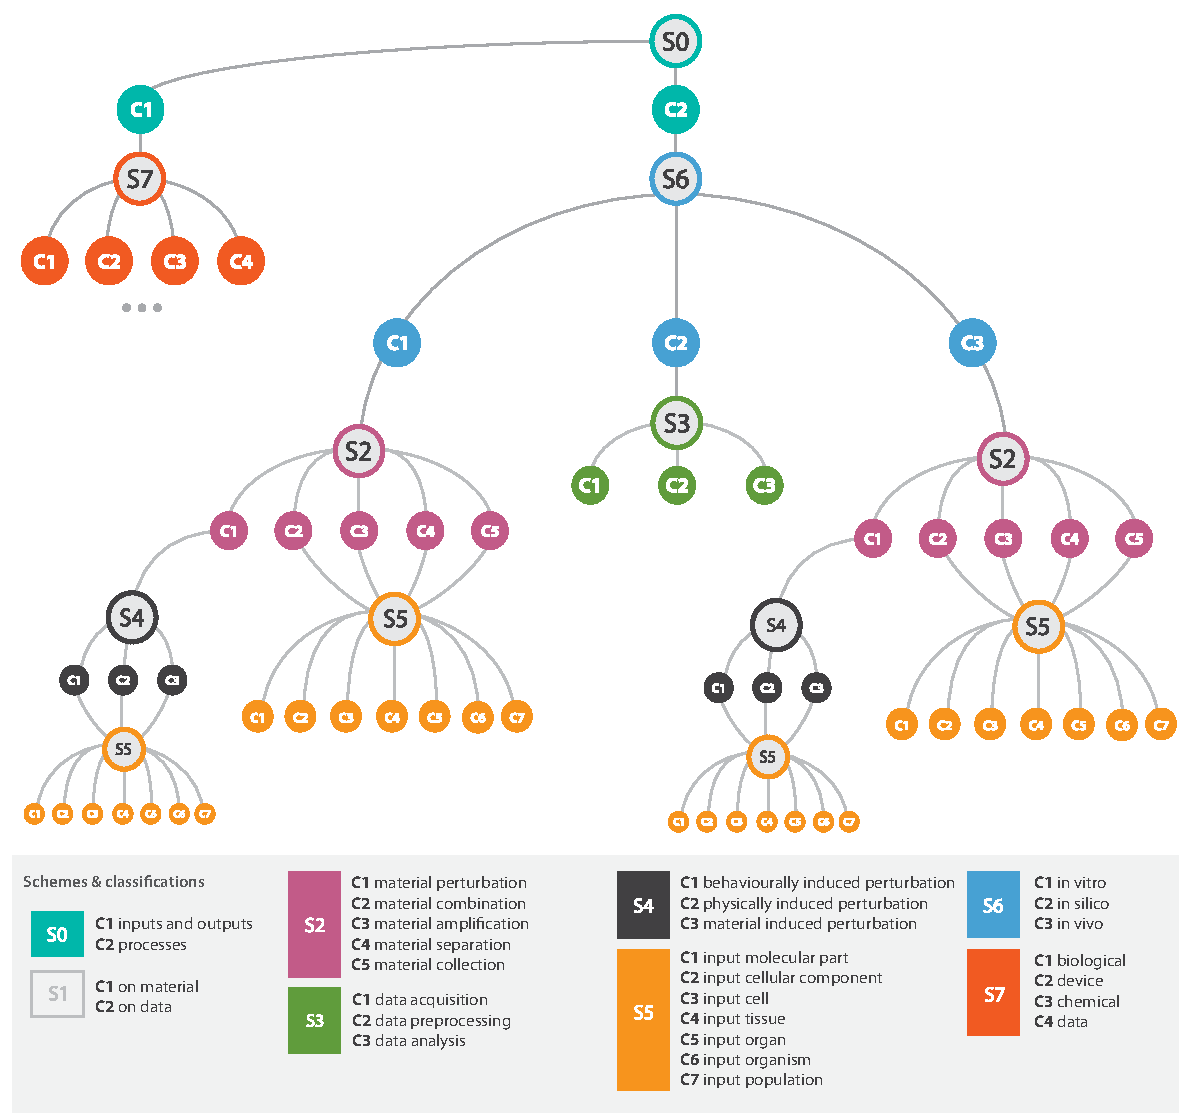
\includegraphics[scale=0.44]{images/glyph-taxonomy/fitness-classification.eps}
\caption{The classification algorithm arranged the classification schemes in the above order.}
\label{fig:fitness-classification}
\vspace{-10pt}
\end{figure}

The creation of the tree shown in Fig. \ref{fig:fitness-classification} was a largely iterative quest with continuous involvement of domain experts checking to ensure that the classifications assigned were meaningful. From early versions of the classification matrix creation, classifications were removed, added or merged in consultation with those who knew the data domain. For example, in \emph{S2} there were sub-classifications in \emph{Genetic Modification \& Labeling} which are types of \emph{Material Combination}. Therefore, these sub-classifications were removed since it would be technically and semantically incorrect to keep them. These early interactions emphasized the importance of having domain experts in the loop, otherwise classifications and subsequent glyphs would not be as well created as they could be.

The algorithm managed to correctly place the classifications where they were expected (checks were made by hand to ensure that the algorithm performed well). Schema \emph{S6} (\emph{in vitro}, \emph{in silico} and \emph{in vivo}) was the best top level classification due to its overall fitness metric of 3.08 with individual metrics found to be: M1 = 1.0; M2 = 1.0; M3 = 0.9; and M4 = 0.18. \emph{S6} was closely followed by \emph{S1} (on material and on data), however after the top level separation, \emph{S1} became redundant as a result of the top level implicitly making a split on data (in silico) and materials (in vitro and in vivo). The algorithm successfully detected this redundancy; hence $S1$ is absent from Fig. \ref{fig:fitness-classification}. 

Although the algorithm performed as expected, a possible criticism of the algorithm could be highlighted in the placement of \emph{S5} below \emph{S4}. \emph{S5} could have been placed above \emph{S4} in line with the observation that, for the majority of cases, \emph{S5} was selected over \emph{S4}. The reason \emph{S5} wasn't used to sub-classify C1 of \emph{S4} is due to its number of classifications (7) being greater than that of \emph{S4} (3), therefore \emph{S4} was selected primarily on this metric even though the sub-tree balance of \emph{S5} (0.8) was slightly better than that of \emph{S4} (0.68). To modify this behavior, it was necessary to involve domain experts in refining the tree based on their domain-specific knowledge and case-specific requirements.

% ---------------------------------------
\begin{table*}[!t]
\centering
\caption{Perceptual strength of different visual channels based on levels of organization studied by Bertin\cite{bertin83} and Green\cite{green98}, `popout' effect studied extensively in psychology \cite{williams67,duncan89,luck94,bertin83,green98,wolfe89,treisman77,palmer77,parkhurst02}, and hierarchy effect studied by Navon \cite{navon77} and Love \cite{love99}. The summary strength of each channel is estimated and it should be considered in conjunction with application-specific conventions and metaphors.}
\vspace{1mm}
\scalebox{0.9}{
\begin{tabular}{|l|l|l|l|l|l|l|c|l|c|}
\hline
 &  \textbf{Visual} & \multicolumn{ 4}{c|}{\textbf{Levels of Organization}} & \textbf{Popout} & \textbf{Hierarchy} & \textbf{Summary} & \textbf{Convention} \\
%
\textbf{Regions} & \textbf{Channels} & \textbf{Associative} & \textbf{Selective} & \textbf{Ordered} & \textbf{Quantitative} & \textbf{Effect} & \textbf{Effect} & \textbf{Strength} & \textbf{\& Metaphor} \\ \hline
%
a) Main & 1. Color & Yes & Yes & Yes & 	& ***** & Strong  & ***** & application \\ \cline{ 2- 7}\cline{ 9- 9}
 & 2. Size &  & Yes & Yes & Yes 		& *** &   & **** &  specific \\ \cline{ 2- 7}\cline{ 9- 9}
 & 3. Shape & Yes & Yes &  &			& *** &   & *** &  \\ \cline{ 2- 7}\cline{ 9- 9}
 & 4. Orientation & Yes & Yes &  & 		& *** &   & *** & \\ \cline{ 2- 7}\cline{ 9- 9}
 & 5.Texture & Yes & Yes & Yes & 		& ** &    & ** &  \\ \cline{ 1- 9}
b) Supplementary & 6-10 (same as 1-5) &  &  &  &  &  & Medium &  & \\ \cline{ 2- 7}\cline{ 9- 9}
 & 11. Planar & Yes & Yes &  & Yes		& *** &  &  *** &  \\ \cline{ 1- 10}
c) Interior & Contains (a+b)) &  &  &  &  &				&  Low &  & \\ \hline
\end{tabular}
}
\vspace{-5mm}
\label{tab:visual-variables}
\end{table*}



%\begin{table*}[t!]

\begin{center}
\scalebox{0.60}{
\begin{tabular}{|l|l|l|l|l|l|l|l|l|l|l|l|l|l|l|l|l|l|l|}
\hline
 &  & \multicolumn{ 5}{c|}{\textbf{\textit{Main}}} & \multicolumn{ 6}{c|}{\textbf{\textit{Supplementary}}} & \multicolumn{ 6}{c|}{\textbf{\textit{Interior}}} \\ \hline
 &  & \textbf{Colour} & \textbf{Size} & \textbf{Shape} & \textbf{Orientation} & \textbf{Texture} & \textbf{Colour} & \textbf{Size} & \textbf{Shape} & \textbf{Orientation} & \textbf{Texture} & \textbf{Planar} & \textbf{Colour} & \textbf{Size} & \textbf{Shape} & \textbf{Orientation} & \textbf{Texture} & \textbf{Planar} \\ \hline
\multicolumn{ 1}{|l|}{\textbf{\textit{Main}}} & \textbf{Colour} & \cellcolor{Gray} & $\gt$\cellcolor{Orange} \cite{williams67,luck94} & $\gt$\cellcolor{Orange} \cite{williams67} & $\gt$\cellcolor{Orange} \cite{luck94, parkhurst02} & Unk\cellcolor{Cream} & $\gt$\cellcolor{Orange} & $\gt$\cellcolor{Orange} & $\gt$\cellcolor{Orange} & $\gt$\cellcolor{Orange} & Unk\cellcolor{Cream} & Unk\cellcolor{Cream} & $\gt$\cellcolor{Orange} & $\gt$\cellcolor{Orange} & $\gt$\cellcolor{Orange} & $\gt$\cellcolor{Orange} & Unk\cellcolor{Cream} & Unk\cellcolor{Cream} \\ \cline{ 2- 19}
\multicolumn{ 1}{|l|}{} & \textbf{Size} & $\lt$\cellcolor{Blue} & \cellcolor{Gray} & $\gt$\cellcolor{Orange} \cite{williams67} & $\gt$\cellcolor{Orange} \cite{williams67,luck94} & Unk\cellcolor{Cream} & $\gt$\cellcolor{Orange} & $\gt$\cellcolor{Orange} & $\gt$\cellcolor{Orange} & $\gt$\cellcolor{Orange} & Unk\cellcolor{Cream} & Unk\cellcolor{Cream} & $\gt$\cellcolor{Orange} & $\gt$\cellcolor{Orange} & $\gt$\cellcolor{Orange} & $\gt$\cellcolor{Orange} & Unk\cellcolor{Cream} & Unk\cellcolor{Cream} \\ \cline{ 2- 19}
\multicolumn{ 1}{|l|}{} & \textbf{Shape} & $\lt$\cellcolor{Blue} & $\lt$\cellcolor{Blue} & \cellcolor{Gray} & $\gt$ \cite{luck94}\cellcolor{Orange} & Unk\cellcolor{Cream} & $\gt$\cellcolor{Orange} & $\gt$\cellcolor{Orange} & $\gt$\cellcolor{Orange} & $\gt$\cellcolor{Orange} & Unk\cellcolor{Cream} & Unk\cellcolor{Cream} & $\gt$\cellcolor{Orange} & $\gt$\cellcolor{Orange} & $\gt$\cellcolor{Orange} & $\gt$\cellcolor{Orange} & Unk\cellcolor{Cream} & Unk\cellcolor{Cream} \\ \cline{ 2- 19}
\multicolumn{ 1}{|l|}{} & \textbf{Orientation} & $\lt$\cellcolor{Blue} & $\lt$\cellcolor{Blue} & $\lt$\cellcolor{Blue} & \cellcolor{Gray} & Unk\cellcolor{Cream} & $\gt$\cellcolor{Orange} & $\gt$\cellcolor{Orange} & $\gt$\cellcolor{Orange} & $\gt$\cellcolor{Orange} & Unk\cellcolor{Cream} & Unk\cellcolor{Cream} & $\gt$\cellcolor{Orange} & $\gt$\cellcolor{Orange} & $\gt$\cellcolor{Orange} & $\gt$\cellcolor{Orange} & Unk\cellcolor{Cream} & Unk\cellcolor{Cream} \\ \cline{ 2- 19}
\multicolumn{ 1}{|l|}{} & \textbf{Texture} & Unk\cellcolor{Cream} & Unk\cellcolor{Cream} & Unk\cellcolor{Cream} & Unk\cellcolor{Cream} & \cellcolor{Gray} & Unk\cellcolor{Cream} & Unk\cellcolor{Cream} & Unk\cellcolor{Cream} & Unk\cellcolor{Cream} & $\gt$\cellcolor{Orange} & Unk\cellcolor{Cream} & Unk\cellcolor{Cream} & Unk\cellcolor{Cream} & Unk\cellcolor{Cream} & Unk\cellcolor{Cream} & $\gt$\cellcolor{Orange} & Unk\cellcolor{Cream} \\ \hline
\multicolumn{ 1}{|l|}{\textbf{\textit{Supplementary}}} & \textbf{Colour} & $\lt$\cellcolor{Blue} & $\lt$\cellcolor{Blue} & $\lt$\cellcolor{Blue} & $\lt$\cellcolor{Blue} & Unk\cellcolor{Cream} & \cellcolor{Gray} & $\gt$\cellcolor{Orange} & $\gt$\cellcolor{Orange} & $\gt$\cellcolor{Orange} & Unk\cellcolor{Cream} & Unk\cellcolor{Cream} & $\gt$\cellcolor{Orange} & $\gt$\cellcolor{Orange} & $\gt$\cellcolor{Orange} & $\gt$\cellcolor{Orange} & Unk\cellcolor{Cream} & Unk\cellcolor{Cream} \\ \cline{ 2- 19}
\multicolumn{ 1}{|l|}{} & \textbf{Size} & $\lt$\cellcolor{Blue} & $\lt$\cellcolor{Blue} & $\lt$\cellcolor{Blue} & $\lt$\cellcolor{Blue} & Unk\cellcolor{Cream} & $\lt$\cellcolor{Blue} & \cellcolor{Gray} & $\gt$\cellcolor{Orange} & $\gt$\cellcolor{Orange} & Unk\cellcolor{Cream} & Unk\cellcolor{Cream} & $\gt$\cellcolor{Orange} & $\gt$\cellcolor{Orange} & $\gt$\cellcolor{Orange} & $\gt$\cellcolor{Orange} & Unk\cellcolor{Cream} & Unk\cellcolor{Cream} \\ \cline{ 2- 19}
\multicolumn{ 1}{|l|}{} & \textbf{Shape} & $\lt$\cellcolor{Blue} & $\lt$\cellcolor{Blue} & $\lt$\cellcolor{Blue} & $\lt$\cellcolor{Blue} & Unk\cellcolor{Cream} & $\lt$\cellcolor{Blue} & $\lt$\cellcolor{Blue} & \cellcolor{Gray} & $\gt$\cellcolor{Orange} & Unk\cellcolor{Cream} & Unk\cellcolor{Cream} & $\gt$\cellcolor{Orange} & $\gt$\cellcolor{Orange} & $\gt$\cellcolor{Orange} & $\gt$\cellcolor{Orange} & Unk\cellcolor{Cream} & Unk\cellcolor{Cream} \\ \cline{ 2- 19}
\multicolumn{ 1}{|l|}{} & \textbf{Orientation} & $\lt$\cellcolor{Blue} & $\lt$\cellcolor{Blue} & $\lt$\cellcolor{Blue} & $\lt$\cellcolor{Blue} & Unk\cellcolor{Cream} & $\lt$\cellcolor{Blue} & $\lt$\cellcolor{Blue} & $\lt$\cellcolor{Blue} & \cellcolor{Gray} & Unk\cellcolor{Cream} & Unk\cellcolor{Cream} & $\gt$\cellcolor{Orange} & $\gt$\cellcolor{Orange} & $\gt$\cellcolor{Orange} & $\gt$\cellcolor{Orange} & Unk\cellcolor{Cream} & Unk\cellcolor{Cream} \\ \cline{ 2- 19}
\multicolumn{ 1}{|l|}{} & \textbf{Texture} & Unk\cellcolor{Cream} & Unk\cellcolor{Cream} & Unk\cellcolor{Cream} & Unk\cellcolor{Cream} & Unk\cellcolor{Cream} & Unk\cellcolor{Cream} & Unk\cellcolor{Cream} & Unk\cellcolor{Cream} & Unk\cellcolor{Cream} & \cellcolor{Gray} & Unk\cellcolor{Cream} & Unk\cellcolor{Cream} & Unk\cellcolor{Cream} & Unk\cellcolor{Cream} & Unk\cellcolor{Cream} & $\gt$\cellcolor{Orange} & Unk\cellcolor{Cream} \\ \cline{ 2- 19}
\multicolumn{ 1}{|l|}{} & \textbf{Planar} & Unk\cellcolor{Cream} & Unk\cellcolor{Cream} & Unk\cellcolor{Cream} & Unk\cellcolor{Cream} & Unk\cellcolor{Cream} & Unk\cellcolor{Cream} & Unk\cellcolor{Cream} & Unk\cellcolor{Cream} & Unk\cellcolor{Cream} & Unk\cellcolor{Cream} & \cellcolor{Gray} & Unk\cellcolor{Cream} & Unk\cellcolor{Cream} & Unk\cellcolor{Cream} & Unk\cellcolor{Cream} & Unk\cellcolor{Cream} & Unk\cellcolor{Cream} \\ \hline
\multicolumn{ 1}{|l|}{\textbf{\textit{Interior}}} & \textbf{Colour} & $\lt$\cellcolor{Blue} & $\lt$\cellcolor{Blue} & $\lt$\cellcolor{Blue} & $\lt$\cellcolor{Blue} & Unk\cellcolor{Cream} & $\lt$\cellcolor{Blue} & $\lt$\cellcolor{Blue} & $\lt$\cellcolor{Blue} & $\lt$\cellcolor{Blue} & Unk\cellcolor{Cream} & Unk\cellcolor{Cream} & \cellcolor{Gray} & $\gt$\cellcolor{Orange} & $\gt$\cellcolor{Orange} & $\gt$\cellcolor{Orange} & Unk\cellcolor{Cream} & Unk\cellcolor{Cream} \\ \cline{ 2- 19}
\multicolumn{ 1}{|l|}{} & \textbf{Size} & $\lt$\cellcolor{Blue} & $\lt$\cellcolor{Blue} & $\lt$\cellcolor{Blue} & $\lt$\cellcolor{Blue} & Unk\cellcolor{Cream} & $\lt$\cellcolor{Blue} & $\lt$\cellcolor{Blue} & $\lt$\cellcolor{Blue} & $\lt$\cellcolor{Blue} & Unk\cellcolor{Cream} & Unk\cellcolor{Cream} & $\lt$\cellcolor{Blue} & \cellcolor{Gray} & $\gt$\cellcolor{Orange} & $\gt$\cellcolor{Orange} & Unk\cellcolor{Cream} & Unk\cellcolor{Cream} \\ \cline{ 2- 19}
\multicolumn{ 1}{|l|}{} & \textbf{Shape} & $\lt$\cellcolor{Blue} & $\lt$\cellcolor{Blue} & $\lt$\cellcolor{Blue} & $\lt$\cellcolor{Blue} & Unk\cellcolor{Cream} & $\lt$\cellcolor{Blue} & $\lt$\cellcolor{Blue} & $\lt$\cellcolor{Blue} & $\lt$\cellcolor{Blue} & Unk\cellcolor{Cream} & Unk\cellcolor{Cream} & $\lt$\cellcolor{Blue} & $\lt$\cellcolor{Blue} & \cellcolor{Gray} & $\gt$\cellcolor{Orange} & Unk\cellcolor{Cream} & Unk\cellcolor{Cream} \\ \cline{ 2- 19}
\multicolumn{ 1}{|l|}{} & \textbf{Orientation} & $\lt$\cellcolor{Blue} & $\lt$\cellcolor{Blue} & $\lt$\cellcolor{Blue} & $\lt$\cellcolor{Blue} & Unk\cellcolor{Cream} & $\lt$\cellcolor{Blue} & $\lt$\cellcolor{Blue} & $\lt$\cellcolor{Blue} & $\lt$\cellcolor{Blue} & Unk\cellcolor{Cream} & Unk\cellcolor{Cream} & $\lt$\cellcolor{Blue} & $\lt$\cellcolor{Blue} & $\lt$\cellcolor{Blue} & \cellcolor{Gray} & Unk\cellcolor{Cream} & Unk\cellcolor{Cream} \\ \cline{ 2- 19}
\multicolumn{ 1}{|l|}{} & \textbf{Texture} & Unk\cellcolor{Cream} & Unk\cellcolor{Cream} & Unk\cellcolor{Cream} & Unk\cellcolor{Cream} & Unk\cellcolor{Cream} & Unk\cellcolor{Cream} & Unk\cellcolor{Cream} & Unk\cellcolor{Cream} & Unk\cellcolor{Cream} & $\lt$\cellcolor{Blue} & Unk\cellcolor{Cream} & Unk\cellcolor{Cream} & Unk\cellcolor{Cream} & Unk\cellcolor{Cream} & Unk\cellcolor{Cream} & \cellcolor{Gray} & Unk\cellcolor{Cream} \\ \cline{ 2- 19}
\multicolumn{ 1}{|l|}{} & \textbf{Planar} & Unk\cellcolor{Cream} & Unk\cellcolor{Cream} & Unk\cellcolor{Cream} & Unk\cellcolor{Cream} & Unk\cellcolor{Cream} & Unk\cellcolor{Cream} & Unk\cellcolor{Cream} & Unk\cellcolor{Cream} & Unk\cellcolor{Cream} & Unk\cellcolor{Cream} & Unk\cellcolor{Cream} & Unk\cellcolor{Cream} & Unk\cellcolor{Cream} & Unk\cellcolor{Cream} & Unk\cellcolor{Cream} & Unk\cellcolor{Cream} & \cellcolor{Gray} \\ \hline
\end{tabular}


}
\end{center}
\caption{Comparison of selected retinal variables available for the glyph design and their expected priority interactions based on review of effects presented in Table 1.
Unk. Unknown: no data documenting the interaction. > superiority/precedence , < inferiority/deference where row value are on the left of the operator and column value is the right term of the the operator.}
\label{tab:visual-variable-strength}
\end{table*}


% ==============
\section{Visual Encoding}
\label{sec:Glyphs}
\subsection{Perceptual Guidance}
%
A \emph{glyph} is a small visual object composed of a number of \emph{visual channels} which can be used independently as well as constructively to depict attributes of a data record.
Glyphs are of a type of visual signs that can make use of visual features of other types of signs, such as icons, indices and symbols.

Although there are several books on sign design (e.g., \cite{barker00,abdullah06}), they focus on signage in public space, and offer empirical guidance on a large number of issues including standardization, size, location, illumination and so on.
Many of these issues are not quite relevant to the need for visualizing the workflows of biological experiments. Here, we draw our design principles mainly from findings in perception, especially in the area of visual search \cite{spoehr82,quinlan03}.

While the extensive use of signs, icons and pictograms in everyday life reflects their usefulness and effectiveness, several perceptual studies also directly or indirectly confirmed their perceptual and cognitive merits.
For example, Franks and Bransford's study on transformation of prototypes \cite{franks71} suggested that humans can learn to recognize glyphs by rules consciously as well as unconsciously.
The presence of iconic memory \cite{sperling60} may facilitate rapid comparison between glyphs in the same display, whereas it is less so for texts.

\textbf{Guideline on Semantic Relevance}.
Bertin \cite{bertin83} classified visual channels (which he referred to as retinal variables) into two categories, planar (location) and retinal (size, color, shape, orientation, texture and brightness).
Bertin proposed four semantic criteria for determining the suitability of different channels in representing certain types of information.
These semantic criteria are: \emph{associative}, \emph{selective}, \emph{ordered} and \emph{quantitative}.
These criteria are important guidelines, though there has been disagreement in the literature as to how individual visual channels are judged.
For example, Bertin considered shape as a non-selective variable.
Research has shown that shapes such as filled rectangles, circles and triangles do not allow the human visual system to identify one shape from another effectively in a rapid action when they form some global structures \cite{love99, navon77}, (they have poor ``pop-out'' effect).
However, the omission of all shapes as a selective visual channel has been challenged, for example, by \cite{treisman88,wang94,green98}, who show practice and familiarity can support selectivity with almost any shape.

\textbf{Guideline on Channel Composition}.
As a glyph is likely to feature a number of visual channels, the constructive composition may affect how individual channels are perceived.
A rich collection of literature on integral and separable dimensions shows that the combined dissimilarity of closely integrated visual channels exhibits Euclidean distance $\sqrt{d^2_a + d^2_b}$ \cite{krantz75,handelt72}, whereas that of separable visual channels exhibits city-block distance $d_a  + d_b$ \cite{burns78,shepard64}. 
The latter is more cost-effective than the former in rule-based encoding of multi-faceted concepts, therefore effective glyph design should encompass a non-conflicting set of separable retinal variables. 

\textbf{Guideline on Pop-out Effects}.
Many classic studies in perception also established the ``power'' of different visual channels in terms of \emph{pop-out effect} (pre-attentive search), and fixation (during attentive search)\cite{healey11}.
The \emph{pop-out effect} is one which allows identification of a target within a few nanoseconds of initial exposure to the visual search space.
A result of several milestone studies focusing on observed response times, the ordering of the four commonly used visual channels follows the consensus: color $\prec$ size $\prec$ shape $\prec$ orientation (e.g.,\cite{williams67,quinlan97,ropinski11}).
The symbol $\prec$ reads as \emph{precedes}. However, the strength of color over the other three channels is generally much more noticeable. 

\textbf{Guideline on Visual Hierarchy}.
%
\emph{Visual hierarchy}, with which the environment and objects around us are arranged is a well documented theoretical framework \cite{palmer77,navon77, love99, kinchla79,bar04}.
However, the literature contains a debate over the ways in which the visual system traverses this hierarchy.
There are four possible ways:
top-down (also called global processing) \cite{navon77};
bottom-up (also called local processing);
middle-out \cite{kinchla79};
and salient features (\emph{e.g., edges, points, colors}) \cite{rumelhart70}.
Because glyphs are relatively small in comparison with a whole visualization, we consider at such a ``localized level'', the top-down and salient features may play more significant roles.
The top-down assumption suggests that when consider a glyph in isolation, its global feature will affect visual search more than its local features.
Salient features are partly addressed by the pop-out effects.

\begin{figure}[t]
\centering
\includegraphics[width=86mm]{images/glyph-taxonomy/glyph-space.eps}
\caption{(a) The glyph template with a main body, an interior region and an exterior region (consisting of 4 sections).
(b) Our final design makes use of the main body and interior region.
The exterior is reserved for future extension.
% As we proceed to lower levels, size will have an impact on visual power\cite{duncan89}.
}
\label{fig:glyph-design}
\vspace{-10pt}
\end{figure}

Based on the above-mentioned perceptual guidance, we considered a generic glyph design template for this work as shown in Fig. \ref{fig:glyph-design}(a).
The template divides a glyph into three regions, namely \emph{main body}, \emph{exterior} and \emph{interior}.
In practice, each region can be divided into 2 or more sub-regions (e.g., a twin body glyph or 4 exterior sections), it is convenient to consider the three regions in abstraction.
The separation of these regions facilitates the basic separation of visual channels based on the composition guideline, while allowing us to consider them individually according to the hierarchy guideline.

In theory, the exterior and interior regions may also be divided into sub-regions in a recursive fashion though in practice this is tightly constrained or discouraged by the very limited display resolution typically available for glyphs.
Similar to the design convention for icons, pictograms are normally featured in the interior region.
The exterior region may be further divided in four sections (top, bottom, left and right).
If glyphs will be connected to form a network or graph (as in this work), the use of these four sections has to take into account the possible incoming and outgoing connections.

Table \ref{tab:visual-variables} summarizes relative merits of some of the most commonly-used visual channels in different regions according to Bertin's categorization, pop-out effects and hierarchy effects.
We estimated the overall discriminating capacity of each channel by using a summary rating in the penultimate column.
We also recognized the importance of the conventions and metaphors in an application.
We will discuss visual metaphors further in Section \ref{sec:Mapping}.
We added the last column to highlight the necessity to consider these in a design process.

It is difficult to establish an accurate ranking order of different visual channels by taking all perceptual effects into account in a quantitative manner.
The state of the art in perception research is yet to provide all evidence needed for a full and conclusive analysis.
Nevertheless, Table \ref{tab:visual-variables} can serve a qualitative guidance to glyph designs in this work, providing an ordering of visual channels in parallel with the ordering of categorization schemes discussed in Section \ref{sec:Taxonomy}.

% ---------------------------------------------------------
\subsection{Mapping Taxonomy to Visual Channels}
\label{sec:Mapping}

For each scheme in the taxonomic tree as shown in Fig. \ref{fig:fitness-classification}, we propose a number of design options.
Fig. \ref{fig:design-options} shows some examples of the proposed designs.
For example, the first column shows the use of colors to encode the classes of a categorization scheme.
The second column shows the use abstract shapes.
Some options convey an abstraction from pictorial representations of classes, and in other cases, we try to establish a metaphoric association between a visual channel and a biological categorization. 

Metaphoric visual representations enable domain-specific encoding using ``natural mapping'' \cite{siirtola05,norman02}. This natural mapping can make it easier for users to infer meaning from the glyph with less effort required to learn and remember them \cite{McDougall00}.
A recent study showed that visual metaphors can aid memorization of the information depicted in a visualization \cite{Borgo12}. However, the same study also showed that visually realistic metaphors 
(those with a lot of detail) may have a negative impact on performance in visual search. Moreover, realistic visual metaphors require a higher pixel resolution, and would lose their discriminating capacity in low resolution conditions. 

\begin{figure}[t!]
\centering
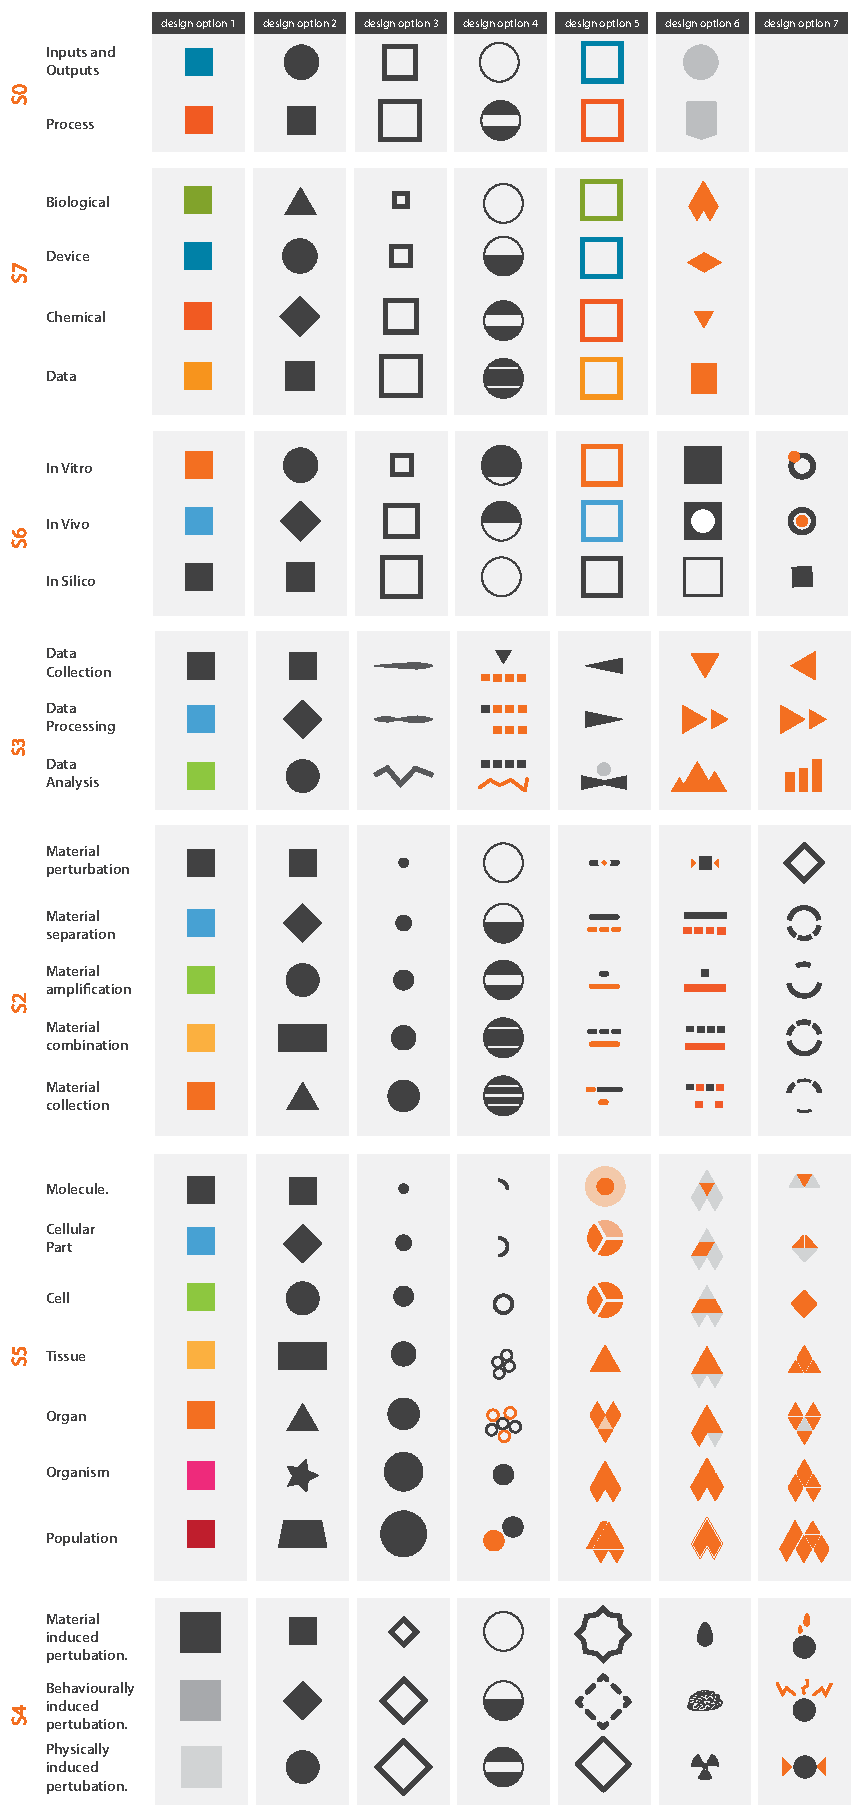
\includegraphics[scale=0.605]{images/glyph-taxonomy/design-options.eps}
\caption{Experimenting with visual channels: an overview of the various design options available for use in representing the different classifications. Most schemes for IO categorization are not shown due to space restriction.}
\label{fig:design-options}
\vspace{-10pt}
\end{figure}

Based on the design options shown in Fig. \ref{fig:design-options}, we followed the taxonomic tree in Fig. \ref{fig:fitness-classification} and identified the best option for each scheme in a hierarchical manner.
The evaluation criteria include:
%
\begin{itemize}
\vspace{-1mm}
\item
the discriminating capacities of different channels (Table \ref{tab:visual-variables});
\vspace{-2mm}
\item
metaphoric capacity for aiding learning and remembering;
\vspace{-2mm}
\item
potential conflicts, including spatial, perceptual and metaphoric conflicts, with visual channels that have already been assigned to other schemes in the tree;
\vspace{-2mm}
\item
encoding costs in terms of requirement for pixel resolution.
\end{itemize}

This process normally takes a few iterations, during which new design options and new metaphoric abstractions and associations are sometimes proposed.

\begin{figure}[t!]
\centering
\includegraphics[scale=0.7]{images/glyph-taxonomy/glyph-design-selection.eps}
\caption{Formation of the final glyph design. Top level items require the greatest visual power. It is important to be able to distinguish each of the processes based on their parent level in the taxonomy. Distinguishable global shapes provide the difference between IOs (circles) and processes (squares with pointed bottom to indicate directionality).}
\label{fig:glyph-design-selection}
\vspace{-10pt}
\end{figure}

Based on the hierarchy in Fig. \ref{fig:fitness-classification}, we considered to use color and shape options for S0 (IOs vs. processes) and S7 (four classes of IOs).
As introducing 4 main body shapes to encode IOs is not an effective mapping for learning and remembering, we decided to assign outline color of the main body to encode S7, and use two basic shapes, circle and pentagon (a rectangle with a pointer to show workflow direction) to encode S0.
Since the main body or the pentagon will only be colored in black or white, S0 also implicitly encoded in using color symbolism, that is, color for IOs and black/white for processes.
In effect, S0 is encoded using two visual channels.
This redundancy can serve as an error detection in visualization \cite{Chen10}.

Fig. \ref{fig:glyph-design-selection} shows each of the five schemes for the process subtree, and the design option chosen from Fig. \ref{fig:design-options}.
Below we discuss our reasoning for selecting each of the design options for each scheme in the taxonomy.


\textbf{S6: Process environment}.
The taxonomic tree suggested a high priority for visual mapping, which is consistent with the domain experts' intuition.
We took advantage that black color was not used by S7 for IOs, we assigned a white background to \emph{in silico/in computer} (related to computational processes), and black to \emph{in vivo/in living)}  and \emph{in vitro/in glass} (related to materials).
Further more, we made use of a shape-based metaphor, fully-filled background for \emph{in vivo} (whole organism), and black background with white cut out for \emph{in vitro} (component of an organism).
Together, this was given in Fig. \ref{fig:design-options} as design option 6.
We maintained the overall appearance of the main body of process glyphs in black and white to avoid potential clash with material glyphs.

\textbf{S2: Types of Material Manipulation}.
S2 has 5 classes, and we adopted design option 7, which employs visual metaphors that encapsulate strong domain-specific meanings.
For example, visual symbol for the \emph{material amplification} class depicts a small segment becoming a large segment.

\textbf{S4: Type of Experimental Perturbation}.
S4 defines 3 further sub-classes of the \emph{material perturbation} class of S2.
Due to the low number of subclasses, we made use of line styles to modify the diamond shape of the \emph{material perturbation}.
We made metaphoric association of three line styles as:
``solid'' line for physically induced perturbation;
dash line, a common metaphor for uncertainty and unpredictability, for behaviorally induced perturbation; and
wavy line, which is closer to a circle (a visual signature for IOs), for material induced perturbation.

\textbf{S5: Levels of Material Granularity}.
This scheme has 7 subclasses (molecule, cellular part, cell, tissue, organ, organism and population), and finding a suitable visual channel was not straightforward. A simplest approach would be to use colors to fill the interior of the glyph, or to use some shape-based encoding.
After consulting the domain experts, these two options were ruled out.
In fact, domain experts preferred some pictograms to represent the 7 subclasses.
After considering a number of more realistic drawings, we found that it was not easy to create realistic representations that can differentiate all subclasses (e.g., cellular part vs. cell; organ vs. organism).
We designed a special set of icons as shown in Fig. \ref{fig:s5-metaphor} with three visual channels to aid learning, memorization and recognition.
The first visual channel is the overall shape and orientation.
The second visual channel is metaphoric abstraction and association.
For example, the shape of cell part indicates a portion of a cell.
Tissue is associated with a patch, organ with an abstract heart shape, organism with an abstract human, population with two abstract humans.
The third visual channel is the number of orange sub-shapes, representing the levels 1-7.
\begin{figure}[t!]
\centering
\includegraphics[scale=1]{images/glyph-taxonomy/s5-metaphor.eps}
\caption{Visual representations of the 7 classes in \emph{S5}.}
\label{fig:s5-metaphor}
\vspace{-10pt}
\end{figure}

\textbf{S3: Types of Data Manipulation}.
S3 defines a 3 further sub-classes of the \emph{in silico} class of S6.
We use three abstract pictograms to represent data capture, processing and analysis. The encoding makes use of the difference in overall shape, orientation, and number of triangles to aid learning, memorization and recognition. Note that these shapes will not be confused with those for S5 as the white background of the main body provides a distinct context of computing rather than IOs.

\begin{figure*}[t!]
\centering
\includegraphics[scale=0.465]{images/glyph-taxonomy/full-tree.eps}
\caption{Overview of the taxonomy based glyph designs in the context of biodomain.}
\label{fig:full-tree}
\vspace{-5pt}
\end{figure*}

Following mapping of all schemes to design options, creation of all glyphs is a straightforward process.
Fig. \ref{fig:full-tree} shows all variations of the glyphs associated with the process sub-tree.

We introduced a ``crush'' test for the designed glyphs by scaling it to different pixel resolutions.
Fig. \ref{fig:crash-test} shows some example glyphs display at varying resolutions.
One can comfortably see all details at the 40$\times$40 level.
At the 10$\times$10 level, one can observe the visual signature of \emph{in vivo} and \emph{in vitro}.
Even at the lowest level (5$\times$5), one can still differentiate the two glyphs. 

\begin{figure}[t!]
\centering
\includegraphics[scale=1]{images/glyph-taxonomy/crash-test.eps}
\caption{A ``crush'' test of glyphs to evaluate the discriminating capacity of various visual channels at different resolutions.}
\label{fig:crash-test}
\vspace{-5pt}
\end{figure}

% ===============
\section{Workflow Visualization and ISA Integration}
\label{sec:Workflow}

In order to visualize workflows of biological experiments, we had to address the following technical issues:
1) mapping from a name in the metadata to a glyph;
2) creating a workflow visualization with both node placement and connection display;
3) developing a prototype tool for a practical environment such as the ISA tools framework.

The mapping from concept name is achieved by a look-up table which is built from the matrix used in formulating the taxonomic tree and implemented as a tab delimited file.
Each concept name is mapped to a text tag encoding the traversal path from the root of the tree to the leaf node corresponding to the name.
The tag includes identifiers of the schemes and classes encountered.
With the path, a glyph can be constructed dynamically from the pre-defined visual mapping as described in the previous section.
The look-up table also enables storage of pre-rendered glyphs in an image format.

To generate the workflow, we made use of the layout algorithm available within the Prefuse visualization framework \cite{heer05}. This framework also brings with it functionality such as panning, zooming and filtering which bring more interactivity to the user and making navigation through large collections of workflows easier. The only requirement for use of Prefuse was a minimal amount of Java code to create the user interface coupled with creation of an XML file format native to Prefuse for representation of the tree structure. This XML format is configurable, we have configured it to contain: \emph{node type} (e.g., process), \emph{node
name} (e.g., labeling) and an image to be rendered, which is assigned using a look-up operation through the above mentioned tab delimited mapping file. The order of the XML elements within this file has direct implications on the order these elements are displayed in. Within the ISA-Tab format, there is an implicit time element found in the ordering of the columns in the study sample and assay files. This can be used to construct the XML elements through near direct mappings of processes and IOs, a workflow which is illustrated in Fig. \ref{fig:generating-workflow-from-text}. Recognizing branching events is an important part of workflow visualization as illustrated in \ref{fig:generating-workflow-from-text}. In software, these branch events can be identified when the preceding nodes of a process have the same names while the succeeding output nodes are different. Fig. \ref{fig:generating-workflow-from-text} highlights one such case, where branching occurs after extraction of 3 materials from one sample. 

Our software reads text-based ISA-Tab files as illustrated to create the XML notations required by Prefuse for rendering the experiment workflow illustrated in Fig. \ref{fig:teaser}(b).

\begin{figure}[t!]
\centering
\includegraphics[scale=.2745]{images/glyph-taxonomy/generating-workflow-from-text.eps}
\caption{A workflow is recorded in text form within the ISA-Tab format.
Our software translates it to glyph-based visualization.
A branching event is automatically detected during the translation.}
\label{fig:generating-workflow-from-text}
\vspace{-10pt}
\end{figure}

\begin{figure}[ht!]
\centering
\includegraphics[scale=.295]{images/glyph-taxonomy/bio-workflow-example.eps}
\caption{User can interact with a workflow to view the text descriptions of individual glyphs in pop-up windows, which are also dynamic legends showing how the concept is categorized and how the corresponding glyph is decomposed into different elementary visual representations. Users can also use such a legend to find out other classes in a categorization scheme.}
\label{fig:bioworkflow-example}
\vspace{-15pt}
\end{figure}

The software is implemented as a Java application capable of processing ISA-Tab files to create experimental workflows using glyphs. For the purposes of broad dissemination in the near future, we have integrated the workflow visualization directly inside ISAcreator, a Java desktop application for creating and editing ISA-Tab files. Furthermore, the standalone workflow visualization shown in figures \ref{fig:bioworkflow-example}a and b makes use of the same ISA-Tab parser as available within ISAcreator. The integration involved the development of user interface elements for ISAcreator software to access the workflow visualization.
From the spreadsheet view, users may highlight rows (assays), right click and select an option named ``View workflow for assays'' to visualize the entire processing pipeline for the corresponding samples as shown in Fig. \ref{fig:teaser}(b).

\section{Conclusions and Future Work}
\label{sec:Conclusion}

Although it was established in psychology that people can learn rules of glyph encoding consciously as well as unconsciously \cite{franks71}, we do not expect users to learn and remember these glyphs without help. We thus allow users to find detailed text descriptions in pop-up windows interactively. As shown in Fig. \ref{fig:bioworkflow-example}, not only do these windows provide names of processes and IOs, they also serve as dynamic legends, showing how each glyph is decomposed into different elements corresponding to categorization schemes. One can also select a component to view all classes in a scheme.   

In this manuscript, we presented a systematic approach for glyph
design by using taxonomy as a guide. We demonstrated our approach by analyzing the content of a biological database and showed how our tree-building algorithm
could be used to take a large collection of concepts and generate a taxonomic tree, which
provides an ordering of a set of categorization schemes (i.e., attribute dimensions).
This enabled us to draw a parallel between the ordering of attribute dimensions with the ordering of visual channels compiled from the perception and visualization literature. 
We involved domain experts in refining the tree as well as in creating metaphoric abstraction and association for glyphs.
This work was followed by development of a prototype tool for glyph-based visualization of experimental design workflows as found in biology.
The prototype is integrated in the ISA suite of tools to be disseminated to users.

We plan to further the present work to include the provision of ``macros'' in workflows in order to make graphs more compact and create dynamic web-based rendering of the workflows using vector graphics.
We also intend to carry out field-based evaluation through ISAcommons, the user community of ISA-tools framework.
Like all potential diagrammatic schemes, we expect that it will take many iterations before it can become a standard.
Nevertheless, the development of an online visualization tool will make such a process more efficient.
               % final (journal style)
%\documentclass[review,journal]{vgtc}         % review (journal style)
%\documentclass[widereview]{vgtc}             % wide-spaced review
%\documentclass[preprint,journal]{vgtc}       % preprint (journal style)
%\documentclass[electronic,journal]{vgtc}     % electronic version, journal

%% Uncomment one of the lines above depending on where your paper is
%% in the conference process. ``review'' and ``widereview'' are for review
%% submission, ``preprint'' is for pre-publication, and the final version
%% doesn't use a specific qualifier. Further, ``electronic'' includes
%% hyperreferences for more convenient online viewing.

%% Please use one of the ``review'' options in combination with the
%% assigned online id (see below) ONLY if your paper uses a double blind
%% review process. Some conferences, like IEEE Vis and InfoVis, have NOT
%% in the past.

%% Please note that the use of figures other than the optional teaser is not permitted on the first page
%% of the journal version.  Figures should begin on the second page and be
%% in CMYK or Grey scale format, otherwise, colour shifting may occur
%% during the printing process.  Papers submitted with figures other than the optional teaser on the
%% first page will be refused.

%% These three lines bring in essential packages: ``mathptmx'' for Type 1
%% typefaces, ``graphicx'' for inclusion of EPS figures. and ``times''
%% for proper handling of the times font family.



%\chapter{Visual Compression of Workflow Visualizations with Automated Detection of Macro Motifs}
\chapter{Glyph-based Visual Compression of Workflows}
\label{chap:automacron}

\begin{chapquote}{L. Ron Hubbard}{``The evolution of knowledge is toward simplicity, not complexity.''}
\end{chapquote}


%% This is how authors are specified in the journal style

%% indicate IEEE Member or Student Member in form indicated below


%\shortauthortitle{Firstauthor \MakeLowercase{\textit{et al.}}: Paper Title}

%% Abstract section.

 % convincing image showing compression of a repetitive sequence in a workflow using macros.
 


%% Uncomment below to disable the manuscript note
%\renewcommand{\manuscriptnotetxt}{}

%% Copyright space is enabled by default as required by guidelines.
%% It is disabled by the 'review' option or via the following command:
% \nocopyrightspace

%%%%%%%%%%%%%%%%%%%%%%%%%%%%%%%%%%%%%%%%%%%%%%%%%%%%%%%%%%%%%%%%
%%%%%%%%%%%%%%%%%%%%%% START OF THE PAPER %%%%%%%%%%%%%%%%%%%%%%
%%%%%%%%%%%%%%%%%%%%%%%%%%%%%%%%%%%%%%%%%%%%%%%%%%%%%%%%%%%%%%%%%

%% The ``\maketitle'' command must be the first command after the
%% ``\begin{document}'' command. It prepares and prints the title block.

%% the only exception to this rule is the \firstsection command
\section{Introduction}

%% \section{Introduction} %for journal use above \firstsection{..} instead


The term ``macro'' is derived from the Greek word \emph{makro} meaning \emph{big} or \emph{far}.
In Computer Science, the term is defined as ``a single instruction that expands automatically into a set of instruction'' \cite{oxforddict}.
It is commonly used as a noun (\eg, a macro), or an adjective (a macro command). 
In schematic diagrams, such as electronic circuit diagrams, data flow diagrams, and control engineering block diagrams, \emph{macros} are commonly used to provide hierarchical concept abstraction as well as visual compression.
Not only can macros facilitate the ``overview first, details on demand'' from Sheiderman \cite{shneiderman96}, but they can also speed up visual search and reduce cognitive load for experienced users, who are knowledgeable about or have become accustomed to the specification of individual macros.
In effect, their functionality bears some resemblance to \emph{acronyms}.

This work is motivated by the need to reduce the visual complexity of biological experiment workflows in an extension to work conducted in the previous chapter.
Such workflows describe the sequence of processes (arranged with respect to a temporal dimension) enacted on biological materials and signals obtained through experimental observations.
Large repositories of experimental data offer a data corpus that can be tapped into for workflow analysis and, more specifically, detection of commonly-used subgraphs (also referred to as \emph{motifs}).
Success in ``compressing" such recurring motifs using macros would significantly reduce the time required for creating, and perhaps more importantly, viewing, and comparing workflows.

When sketching out workflows on paper, individual scientists often abstract a commonly performed sequence of steps into a macro procedure or represent a set of parallel steps by using a macro step.
Such a macro encapsulates the sense of a bigger block, a higher-level abstraction, and multiple steps, just like in programming and other schematic diagrams.
Despite the potential benefits of using macros, one major stumbling block that hinders the availability and use of macros in workflow visualization is the lack of standards.
Nevertheless, steps towards standardisation can be taken.
With the availability of large collections of workflows in biological experiment repositories, computational approaches may be applied to detect commonly-used motifs (\emph{i.e.}, topological patterns in workflows).
It provides domain experts with an objective means for establishing a list of candidate macros based on their usage.
The final selection of macros can be determined semantically in traditional ways (\eg, community consensus, popularity ranking or recommendations by standards bodies).

The main contributions of this work are as follows:

\begin{itemize}
\vspace{-2mm}
\item Our overall approach for using a computational methodology to identify candidate macros in relation to a workflow repository is new. This enables exhaustive search and objective selection of candidates while still allowing domain experts to make the final decision on macro creation.
\vspace{-2mm}
\item We propose an efficient algorithm for extracting motif patterns in workflows by taking into account node and edge types. This enables motif grouping through inclusion of semantic context. Our tests show that this type-sensitive algorithm performs faster than existing generic algorithms in the literature; and
\vspace{-2mm}
\item
Our motif extraction algorithm is based on a finite-state machine.
As workflows are directional and acyclic, the state transitions for identifying a motif encode the structure of the motif. We make use of such information to characterise the structural pattern of selected macros visually. This facilitates partial automation when designing an individual glyph for each macro. 
\end{itemize}

\section{Related Work}
Schematic representations of workflows are commonplace in a range of disciplines.
A workflow typically describes a sequence of steps, followed from initiation to completion when conducting a piece of work.
Perhaps the most widely used workflow visualization is the \emph{Gantt chart}, which depicts tasks, resources, and their dependencies in a temporal manner.
Efforts such as \emph{VisTrails} \cite{callahanvistrails:2006}, \emph{VTK} \cite{schroederthe1996} and \emph{SmartLink} \cite{teleasmartlink:2000} make use of workflows to depict the processes followed to create a visualization.
In \emph{Taverna} \cite{hull06} and \emph{Kepler} \cite{altintaskepler:2004}, workflow visualization is used to facilitate construction of reproducible pipelines for data analysis.  
Other workflow visualizations include the Business Process Model and Notation (\emph{BPMN}), Petri-net, and programming flowchart, all of which convey work flow, data flow, and process interactions within often very complex systems. 

In this work, we consider workflows used to describe biological experiments.
This class of workflow visualization renders the processes
enacted on biological materials in experimental setups, from sample collection through experimental perturbation to signal acquisition and interpretation.
While most scientists have been using generic text-based graph drawing tools such as \emph{GraphViz} \cite{GraphViz::2012}, new workflow visualization tools, such as that shown in Chapter \ref{chap:glyph-tax} are emerging. 

% improve link between the previous section and this one.
\emph{Graph reduction} is a family of algorithms and techniques for reducing visual complexity by using graph filtering and graph aggregation \cite{landesberger11}.
\emph{Graph filtering} involves removal of certain nodes and edges from the graph, either deterministically or stochastically \cite{leskovec06,landesberger11}.
\emph{Graph aggregation} selectively merges two or more nodes into one, hence preserving some information about the nodes and edges to be removed.
Many selection algorithms exist, such as methods for building hierarchical levels of detail, clustering based on node/edge attributes and edge bundling for clutter reduction \cite{landesberger11,holten06}.

One subset of graph reduction techniques is motif based.
Motifs, in the context of graphs, are ``patterns of interconnections occurring in complex networks'' \cite{Milo:2002,Pavlopoulos:2011}.
% Motifs with similar features have been observed in diverse domains, ranging from electronics and biological networks to food webs \cite{Pavlopoulos:2011}. 
A considerable amount of effort has been dedicated to the automatic identification and characterisation of motifs in individual graphs or sets of graphs.
Examples include \emph{mfinder} by Kashtan \etal \cite{kashtan04}, \emph{FANMOD} from Wernicke and Rashe \cite{wernicke06}, and \emph{mavisto} from \cite{schreiber05}.
Replacing recurring motifs with macros can provide hierarchical concept abstraction, visual compression, improved readability, and cost-effective task performance.
Macros feature extensively in various graph representations, such as schematic diagrams, communication network diagrams, and workflow diagrams.
For example, \emph{VisMashup} \cite{santosvismashup:2009} utilises macros to simplify the large body of steps required to create a visualization.
Dunne and Shneiderman propose to simplify graphs by using fan and arced glyphs to represent common topological structures \cite{dunnemotif2012}.
Shneiderman and Aris propose the use of user-defined semantic substrates for compressing network visualization \cite{Shneiderman:2006:TVCG}. 
However, determining suitable macros usually depends on both the semantic content of the corresponding motif and its potential use in graph reduction.
Hence, relying solely on topological information may not lead to meaningful visualizations, while relying solely on user input does not scale up to a large collection of graphs.

\begin{table}[!t]
\centering
\scalebox{1}{
\begin{tabular}{|l|c|c|c|}
\hline
\textbf{Algorithm} & \textbf{Sampling} & \textbf{Node Limit} & \textbf{Focus} \\ \hline
mfinder \cite{kashtan05} &
  exact \& estimated & 6 & discovery \\ \hline
FPF (mavisto) \cite{schreiber05} &
  exact & 4 & search \\ \hline
FANMOD \cite{wernicke06} &
  exact \& estimated & 8 & discovery \\ \hline
NeMoFinder \cite{chen06} &
  exact & 12 & search \\ \hline
MODA \cite{omidi09} &
  exact & not defined & search \\ \hline
G-Tries \cite{ribeiro10} &
  exact & $>$ 9 & discovery \\ \hline
Grochow-Kellis \cite{grochow07} &
  exact & 9 & search \\ \hline
Kavosh \cite{kashani09} &
  exact & 8 & discovery \\ \hline
Colour-coding \cite{Alon:2008} &
  estimated & 10 & discovery \\ \hline
\end{tabular}
}
\caption{Some commonly used motif finding algorithms, and their sampling method.}
\label{tab:motif-algorithms}
\end{table}

\begin{figure}[t!]
\centering
\includegraphics[width=.8\textwidth]{images/automacron/algorithm-differences.eps}
\caption{A) A graph, with typed nodes and edges, where different node types are mapped to different shapes and colours.
B) Generic motif discovery (or search) algorithms focus on topological differences.
C) Our motif extracting algorithm takes varying node/edge types into account, yielding semantically aware motif grouping.
}
\label{fig:new-algorithm-considerations}
\end{figure}

As shown in Table \ref{tab:motif-algorithms}, many motif search/discovery algorithms exist. 
Ribeiro \emph{et al.} \cite{ribeiro10}, Kashani \emph{et al.} \cite{kashani09} and Wong \emph{et al.} \cite{Wong:2012} published benchmarks detailing processing time for a subset of the algorithms in Table \ref{tab:motif-algorithms}.
As subgraph matching is fundamentally an \emph{NP}-complete problem, these algorithms are computationally intensive.
Wong \emph{et al.} report \emph{maVISTO} taking 14,000 seconds to find size three motifs in an \emph{E. Coli} network.
Comparing that to one second for \emph{FANMOD} to analyse the same network, one can see the huge variability in algorithm performance.
As the size of the target motifs grow, performance decreases.
Using the same \emph{E. Coli} network but searching for size 8 motifs, \emph{FANMOD} will need 9,000 seconds to finish the operation \cite{Wong:2012}.

In Table \ref{tab:motif-algorithms} the second column indicates whether the sampling is exact (enumerating all possible candidates) or estimated.
The third column indicates the maximum number of nodes in a motif the algorithm can handle.
The final column indicates whether the algorithm is focused on \emph{motif discovery} (finding repetitive patterns in a set of graphs), or \emph{motif search} (finding a given motif in a set of graphs). 
All algorithms focus on topological patterns in graphs only and do not consider the types of nodes and edges as a search constraint. 
However, the types, or semantic categories of nodes and edges are an interesting property in defining a macro.
There is a more semantically aware motif search algorithm implemented in \emph{VisComplete} \cite{scheideggerquerying2007,koopviscomplete:2008} that compares node labels and node order to predict the next step in a \emph{VisTrails} pipeline analysis over a larger corpus of pipelines.
However this algorithm is topologically less sensitive and provides no way to identify branch/merge events in a motif, or edge types.
A potentially useful algorithm for identifying suitable candidate macros should be type \emph{and} topology sensitive.
This chapter focuses on work to devise such an algorithm, offering additional advantages in computational performance and providing visual mappings with meaningful structural information. 

In our work, when considering whether a subset of steps in a given workflow is the same as another subset in the same or a different workflow, we must consider the semantics attached to each step (see Figure \ref{fig:new-algorithm-considerations}).
Consequently, the task of motif discovery and search is highly constrained by the types of nodes and edges.
Therefore, it is necessary, as well as advantageous, to develop specific motif extraction algorithms for workflow visualizations.
In addition, we propose a novel concept of partially automating the design of macro glyphs.
We consider the use of multi-resolution glyphs to depict macros at different levels of detail when a user interacts with the visualization, a technique referred to by Bederson and Hollan \cite{bedersonpad:1994} and later by Weaver \cite{weaverbuilding2004} as semantic zooming. 

% ==============================
\section{Motivation and System Overview}
\label{sec:Motivation}

Over the past two decades, Biology has benefited from entering the digital era, becoming a data intensive field.
Ancillary to this development, important efforts have been undertaken to preserve and curate digital artefacts in biology, including experimental workflows.
A workflow is a form of directed graph (digraph).
Scientists mainly rely on two types of workflow visualization: digraphs with text labelled boxes or glyph nodes.
The latter enables more compact visual representation than the former \cite{Maguire:2012:TVCG} allowing domain experts to perform their tasks such as error checking and comparison more quickly.
However, workflows can still be quite large and complex, containing many repeated subgraphs, which demand some effort for identification in ``flat'' representations.  
Hence, it is highly desirable to introduce macro representations in workflow visualizations, as both text-based and glyph-based workflow visualizations can benefit from macro-based visual compression.
Although experimental workflows in biology exhibit specific properties that are different from workflows in other disciplines, they often share some characteristics.
Almost all exhibit temporal ordering and most feature only acyclic digraph topologies.
We are therefore hopeful that our algorithm and experience can be transferred to workflow visualizations in other disciplines.

The domain experts involved in this work identified the following requirements: 

\vspace{-2mm}
\begin{enumerate}[itemsep=-1mm]
\item Given a number of workflows, can we obtain the most common patterns/motifs within those workflows?
\item For each motif, can we obtain the occurrence frequencies for that motif and information about which workflows they occur in?
\item Can we automatically create macro representations of those motifs, with the possibility of adding extra annotation to them?
\item Can motif patterns in a workflow be substituted by common macros to make the workflow more compact?
\end{enumerate}

\vspace{-1mm}
Depending on discipline and requirements, macros may be created by individuals based on their own knowledge about needs and usage.
However, such an individualised approach would be impractical if applied to the curation of large collections of experimental workflows as found in data repositories.
Yet, the availability of such data provides an opportunity for the computational identification of commonly occurring motifs in workflows.
The statistics of such motifs offer useful guidance to motif selection when defining macros.

To carry out this work, information was extracted from a curated resource currently holding over 22,000 experimental design workflows (ArrayExpress \cite{ArrayExpress::2012}).
We used a subset of this collection, comprising 9,670 workflows considered to be well-formed with respect to correct connectivity and semantic annotation.
This subset of workflows, available in the ISA-Tab format \cite{rocca-serra10, sansone12}, offers a good representation of experiment typology.
These ISA-Tab files were processed and transferred to a graph database, which provides an optimised environment for storing graph structures and a query language optimised for graph traversal \cite{batra12}. 
For this purpose, we selected \emph{Neo4j} \cite{Neo4J::2012} -- a freely available graph database providing a query language called Cypher, fast traversal algorithms and high scalability (up to several billions of nodes and edges on a single computer).

\begin{figure}[h!]
\centering
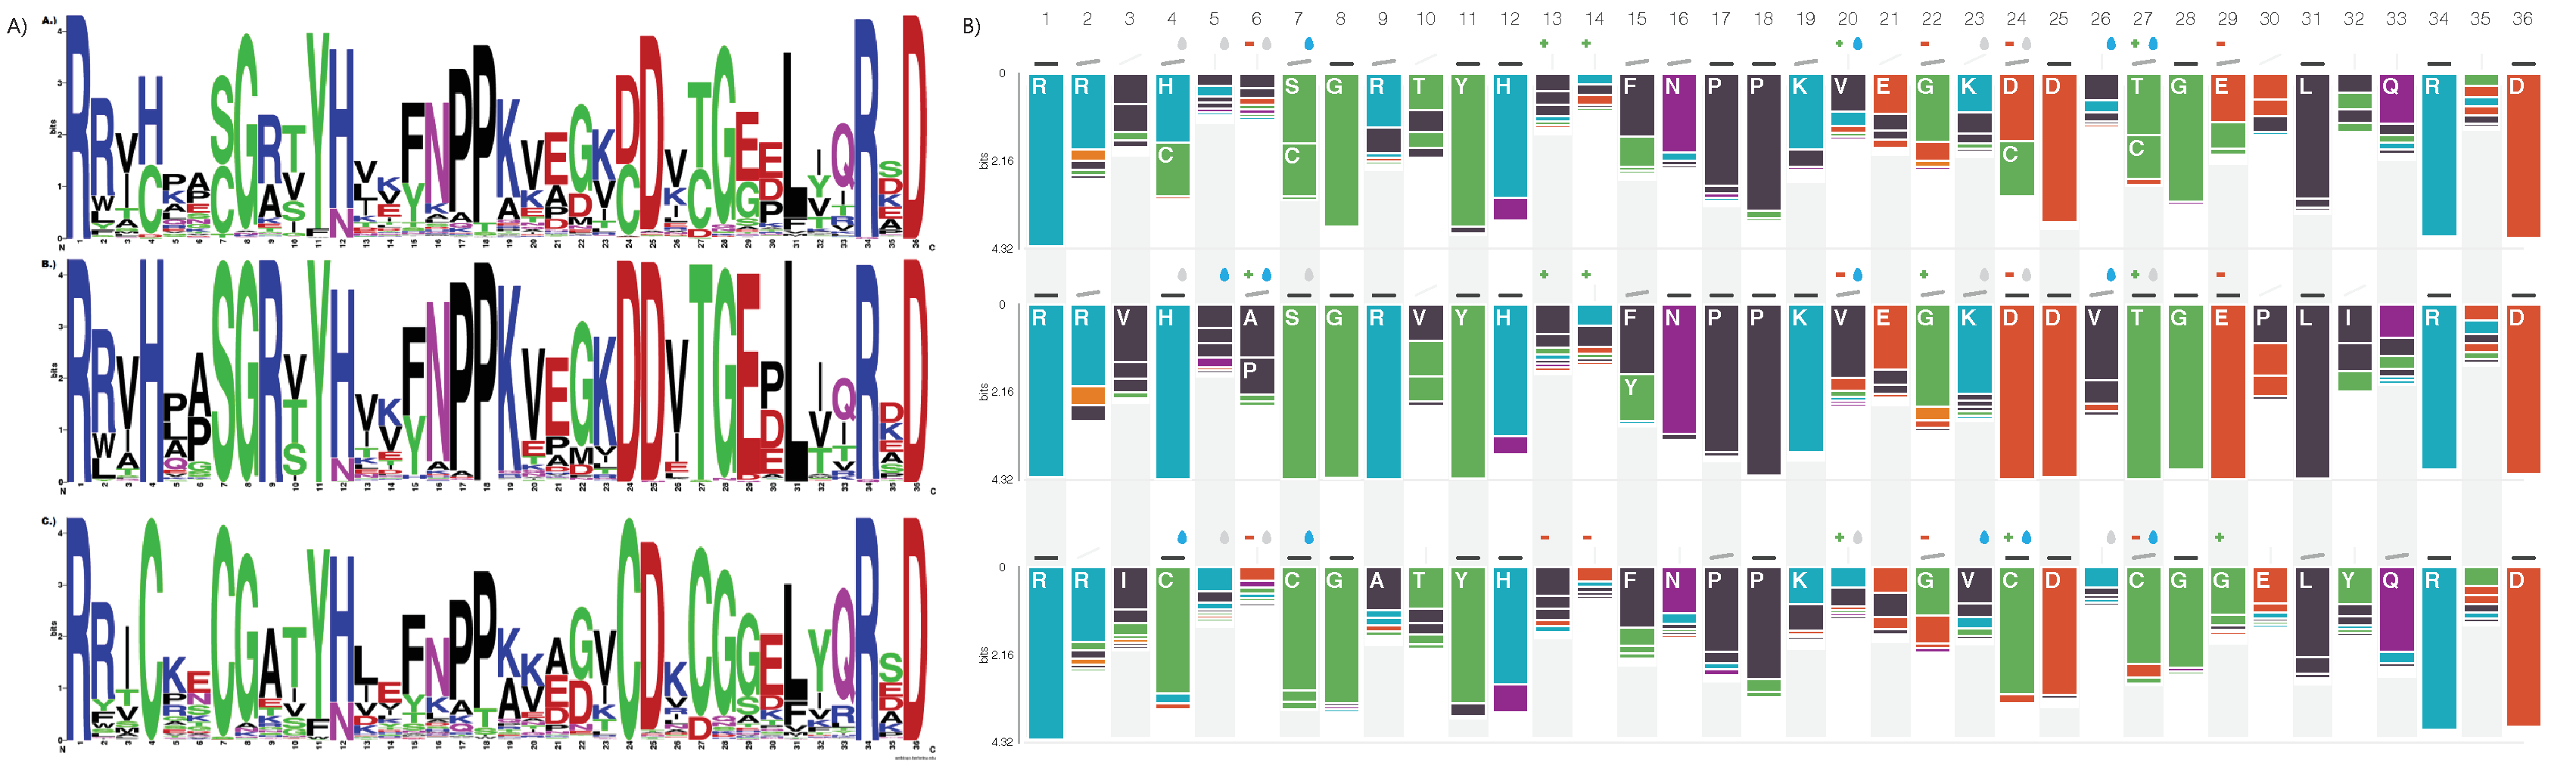
\includegraphics[width=\textwidth]{images/automacron/teaser}
\caption{An overview of the processes implemented in our system, AutoMacron, for compression of workflow visualizations. A) Biological workflows are imported from public repositories. B) The database of workflows is analyzed by our novel motif extraction algorithm that is sensitive to node/edge types and is built using a state-transition approach. C) The algorithm generates a large list of motifs. D) The motifs are ranked using metrics measuring their overall occurrence, scope of influence and compression potential. E) Based on the ordered recommendations by the system as well as their own knowledge, domain experts explore the space of motifs to identify suitable `macros'. F) A subset of motifs are selected for macro generation. G) A glyph is assigned to each macro automatically using a design pattern that utilizes the state output from the motif extraction algorithm. H) Domain experts are able to annotate macros with additional text labels. I) Macros can be inserted into the relevant workflows as a method for graph compression.}
\label{fig:automacron-teaser}
\end{figure}

Our system consists of a number of steps, as depicted in Figure \ref{fig:automacron-teaser}.
\begin{itemize}
\item \textbf{Step 1} (B, C, D) - we algorithmically scan all workflows in the collection and extract all valid subgraphs as candidate motifs.
The patterns and occurrence statistics of these motifs are recorded.
The definition of validity and the extraction algorithm will be detailed in Sections \ref{sec:Conditions} and \ref{sec:automacron_algorithm}.
\item \textbf{Step 2} (E, F) - we provide a user interface for domain experts to define macros by selecting motifs from an ordered list of candidates, based on the statistics computed as well as their domain knowledge about individual motifs and the context of their usage.
This will be discussed in detail in Section \ref{sec:Selection}.
\item \textbf{Step 3} (G, H) - we provide an automatic means for defining the pictogram of a macro by making use of the state transition information captured by the algorithm during the motif discovery phase.
In addition, each macro will normally be displayed with a text label, which is defined by the domain expert through the user interface.
The mechanism for automatic creation of a pictogram will be detailed in Section \ref{sec:Design}.
\item \textbf{Step 4} (I) - we created a tool to allow for substitution of frequent motifs with their macro counterparts in experimental workflows.
This functionality can be accessed via a standalone software package or through an API.
\end{itemize}

% ===============================
\section{From Motifs to Macros}
\label{sec:Motif}

Motif discovery and substitution in graphs typically consists of four processes. These are defined by Milo \etal \cite{Milo:2002} and Alon \cite{Alon:2007} as:

\vspace{-2mm}
\begin{enumerate}[itemsep=-1mm]
\item \emph{Subgraph Generation}: Scan each graph for all possible $n$-node subgraphs.
\item \emph{Motif Amalgamation}: Group together subgraphs that are topologically equivalent and generate a representative subgraph of each group (a motif).
\item \emph{Macro Selection}: Assign a significance value to each motif with respect to other motifs in the collection (for instance, by computing frequency of occurrence) and select the most significant motifs as macros.
\item \emph{Macro Substitution}: Search graphs for subgraphs that match with macros and replace them with that macro.
\end{enumerate}

\vspace{-1mm}
In applications such as biological network rendering, it can be safely assumed that subgraphs should be connected.
By contrast, in applications such as very-large-scale integration (VLSI) design, such a condition is sometimes relaxed, as macros are often used to group elements for a cost-effective spatial placement.
In general, the number of subgraphs can be rather large.
That is why many algorithms only deal with small subgraphs, such as the 4-node subgraphs studied in \cite{Milo:2002}.


\subsection{Candidate Macros in Workflows}
\label{sec:Conditions}
%
The workflows and macros considered in this work exhibit the following characteristics: 

\begin{enumerate}[itemsep=-1mm]
\item A workflow is an acyclic digraph.
\item A macro must consist of at least two nodes.
\item Macros are not only topologically sensitive, but also semantically sensitive. In other words, two subgraphs are said to be in the same motif group only if they are isomorphic and every pair of corresponding nodes (and edges) are of the same type.
\item It is not necessary to have a path between every pair of nodes in a motif.
\item For each node in a macro, there must exist a path from the macro's input node, and a path to the macro's output node.
\item Each macro must have a single input type and a single output type (including \emph{bundled} input and output).
\item A bundled input or output may contain any number of connection edges, but they must be of the same material type.
\item A macro may receive a bundled input converging from different preceding nodes and may deliver a bundled output branching off to different successive nodes.
\end{enumerate}

\begin{figure}[t!]
\centering
\includegraphics[scale=.6]{images/automacron/valid-invalid-motifs.eps}
\caption{In a workflow graph, some subgraphs can be considered as ``legitimate motifs'' while others cannot, depending on node type. Invalid motifs do not have the same output node type, as indicated by the differing colours. Conversely, valid motifs are those that have the same input and output node type.}
\vspace{-3mm}
\label{fig:Conditions}
\end{figure}


By relying on these characteristics we can significantly reduce the number of subgraphs and motifs to be extracted in the \emph{motif generation} stage of the algorithm.
Figure \ref{fig:Conditions} illustrates those subgraphs that are ``legitimate'' candidates and others that are ``illegitimate''.
In addition, owing to characteristic three described above, the \emph{Motif Amalgamation} and \emph{Macro Substitution} stages are much less onerous in comparison to subgraph matching based on topology only. 

% ---------------------------
\subsection{Motif Generation}
\label{sec:automacron_algorithm}
%
\begin{figure}[t!]
\centering
\includegraphics[width=.65\textwidth]{images/automacron/Transition.eps}
\caption{The full space of states and transitions between them encountered during motif generation.}
\label{fig:Transitions}
\end{figure}

\begin{figure*}[t!]
\centering
\begin{tabular}{@{}ccc@{}}
\includegraphics[width=37mm]{images/automacron/States1.eps}&
\includegraphics[height=37mm]{images/automacron/States2.pdf}&
\includegraphics[height=37mm]{images/automacron/States3.eps}\\
A) singular branching & B) homogeneous branching & C) heterogeneous branching
\end{tabular}
\caption{Examples of state transitions with different rules. Homogeneous edges are depicted by using the same colour.}
\label{fig:States}
\end{figure*}

Owing to the aforementioned conditions that are specific to workflows, we could not make use of existing motif generation software and algorithms such as those surveyed in \cite{Wong:2012}.
A specialised motif generation algorithm was needed, and for that we adapted the widely accepted ``pattern growth'' approach \cite{Wong:2012}.
We describe the algorithm by evolving a state transition diagram as shown in Figure \ref{fig:Transitions}.

\noindent \textbf{Singular Branching (Rule A).}
%
As shown in Figure \ref{fig:States} A), the simplest workflow is perhaps a single path composed of $n$ different steps (\eg, experimental steps).
The algorithm can be activated from any node and will only move forward, following the flow of the work.
Since a single node cannot be a macro, the search will park at state $\mathsf{S}_0$ as illustrated in Figure \ref{fig:States} A), where the orange background indicates a starting state and the dotted outline implies that it is only a holding state and does not output a ``legitimate motif''.

When the algorithm encounters the next node $n_1$, it obtains the first ``legitimate motif'', $m_1 = \langle n_0 \rightarrow n_1 \rangle$, and moves to the state $\mathsf{S}_0$.
The edge is labelled with $A$ indicating that this follows rule \textbf{A}.
From $n_1$, the algorithm then encounters $n_2$, it outputs another motif $m_2 = \langle n_0 \rightarrow n_1 \rightarrow n_2 \rangle$, and remains at the same state.
For the workflow in Figure \ref{fig:States} A), this self-loop continues to generate motifs in growing sizes until the end of the path or the number of nodes in the motif reaches a predefined maximum. 

\noindent \textbf{Homogeneous Branching (Rules B, C, D).}
%
One extension of the singular branching case is multiple runs of the same sequence of steps, in parallel.
When the work flows forward, the same type of edges connect to the next set of nodes (see condition 7 in Section \ref{sec:Conditions}).

When an edge first branches to multiple nodes, as illustrated in Figure \ref{fig:Transitions}, the algorithm moves from state $\mathsf{S}_0$ or $\mathsf{S}_1$ to $\mathsf{S}_3$, following a transition of singular branching to bundled homogeneous branching.
This is referred to as rule \textbf{B}.
$\mathsf{S}_3$ indicates more than one edge is being bundled at this state and the number of edges may vary.

The algorithm will self-loop as long as the motif grows with such bundled edges.
Rule \textbf{C} indicates a transition within the state of homogeneous branching.
The number of edges in an edge bundle can change as long as there is more than one edge and they are of the same type.

When all bundled branches converge to a single node, the algorithm returns to state $\mathsf{S}_1$.
This transition is referred to as rule \textbf{D}.
Figure \ref{fig:States} B) shows three examples of applying rules \textbf{B}, \textbf{C} and \textbf{D} respectively.
Applying any of the three rules will result in a bigger motif than the previous one.

An additional state $\mathsf{S}_2$ is included for a scenario when the algorithm starts with a row of parallel nodes with bundled input and output.
We will discuss this scenario later in the context of reactivating the algorithm for bundled edges.

\noindent \textbf{Heterogeneous Branching (Rules E, F, G, H).}
%
Recall conditions 6 and 7 in Section \ref{sec:Conditions}: a macro must have a single input and single output and each can be bundled edges of the same material type.
When these two conditions are met, we can have heterogeneous flow within a macro.
This subset of rules is designed to ``grow'' this particular type of motif.

Rule \textbf{E} is applied when the algorithm first encounters an heterogeneous pattern.
This transition leads to a holding state $\mathsf{S}_4$ and it does not generate any motif.
In this state, all nodes scanned so far are grouped as an interim pseudo-motif and output edges are placed in an interim pseudo-bundle.

The interim state is maintained by a self-loop transition; \emph{i.e.}, rule \textbf{F} as long as the bundled edges remain heterogeneous.
When the edges in an interim pseudo-bundle finally converge to a single node or a set of nodes with homogeneous output edges, the algorithm can leave the holding state $\mathsf{S}_4$.
Rule \textbf{G} defines the transition to singular branching state $\mathsf{S}_1$, while rule \textbf{H} defines the homogeneous branching state $\mathsf{S}_3$.
Both rules will generate a new motif, which includes all nodes in the interim pseudo-motif and the newly encountered node(s).

\noindent \textbf{Termination and Reactivation.}
%
The algorithm strictly follows the breadth-first search strategy.
It may terminate in two situations:
(a) when the predefined maximum depth that a macro may be at is reached;
(b) when it encounters a node without an output edge (\emph{i.e.}, the termination point of a workflow).
The termination condition is tested in all states in Figure \ref{fig:Transitions}.

It is necessary to reactivate the algorithm by choosing each of the different nodes in a workflow as a starting node at state $\textsf{S}_0$.
In addition, each bundle of edges of the same material type can also be a starting point at $\textsf{S}_2$.
Although theoretically appropriate, invoking the algorithm recursively from a starting node of a workflow proved not to be feasible in practice.
We therefore made use of a queue, which initially contains all nodes in a workflow.
We fetch nodes from the queue one at time to invoke the algorithm from $\textsf{S}_0$.
Every time the algorithm reaches state $\textsf{S}_3$, we have a set of homogeneous nodes that were just encountered (\eg, $[n_{1a}, n_{1b}, n_{1c}]$ in Figure \ref{fig:States} B)).
We store all $k$-node subsets of such a set ($k = 2, 3, \ldots$) in a list.
When we finish with all individual nodes in the queue, we sort the list and remove redundant subsets.
We then invoke the algorithm with the sorted and cleaned list from $\textsf{S}_2$.
Note that each subset in the list is a ``legitimate motif'', hence $\textsf{S}_2$ is not a holding state.


% I have to add in the stuff from my meeting with Min here further qualifying why we devised our own algorithm. 

\noindent \textbf{Performance.} To evaluate the performance of the algorithm, we tested it against nine graphs representing biological workflows of varying sizes on a MacBook Pro with a 2.53GHz Intel Core i5 CPU and 8GB RAM.

\begin{figure}[t!]
\centering
\includegraphics[width=.75\textwidth]{images/automacron/workflow-size.eps}
\caption{Scatter plot showing the distribution of workflows (each depicted as a point) as node count versus edge count.}
\vspace{-4mm}
\label{fig:workflow-size}
\end{figure}


The nine graphs were divided into three groups, three small, three medium and three large, based on their node and edge counts.
Figure \ref{fig:workflow-size} shows the distribution of workflows in our collection in terms of nodes ($x$-axis) and edges ($y$-axis).
93\% of all workflows have a node count below 1,000 and the average number of nodes per workflow is approximately 322.
Given these statistics, we define \emph{small} as 200 nodes or below (covering 58\% of workflows); \emph{medium} between 201 and 600 nodes (covering a further 28\% of workflows); and \emph{large} over 601 nodes (covering the remaining 14\%). 

\begin{table}[t!]
\centering
\vspace{1mm}
\scalebox{0.8}{
\begin{tabular}{|l|r|r|r|r|r|}
\hline
\textbf{Graph Size} & \multicolumn{1}{l|}{\textbf{Motif Depth}} & \multicolumn{1}{l|}{\textbf{G1}} & \multicolumn{1}{l|}{\textbf{G2}} & \multicolumn{1}{l|}{\textbf{G3}} & \multicolumn{1}{l|}{\textbf{Seconds}} \\ \hline
 \multicolumn{ 1}{|l|}{} & 3 & 0.018 & 0.017 & 0.024 & 0.02 \\ \cline{ 2- 6}
\multicolumn{ 1}{|l|}{} & 4 & 0.034 & 0.026 & 0.025 & 0.03 \\ \cline{ 2- 6}
\multicolumn{ 1}{|l|}{} & 5 & 0.048 & 0.038 & 0.042 & 0.04 \\ \cline{ 2- 6}
\multicolumn{ 1}{|l|}{} & 6 & 0.059 & 0.041 & 0.046 & 0.05 \\ \cline{ 2- 6}
\multicolumn{ 1}{|l|}{Small} & 7 & 0.075 & 0.049 & 0.049 & 0.06 \\ \cline{ 2- 6}
\multicolumn{ 1}{|l|}{} & 8 & 0.086 & 0.063 & 0.06 & 0.07 \\ \cline{ 2- 6}
\multicolumn{ 1}{|l|}{} & 9 & 0.095 & 0.064 & 0.062 & 0.07 \\ \cline{ 2- 6}
\multicolumn{ 1}{|l|}{} & 10 & 0.106 & 0.069 & 0.072 & 0.08 \\ \hline
\multicolumn{ 1}{|l|}{} & 3 & 0.153 & 0.065 & 0.056 & 0.09 \\ \cline{ 2- 6}
\multicolumn{ 1}{|l|}{} & 4 & 0.212 & 0.097 & 0.085 & 0.13 \\ \cline{ 2- 6}
\multicolumn{ 1}{|l|}{} & 5 & 0.24 & 0.13 & 0.115 & 0.16 \\ \cline{ 2- 6}
\multicolumn{ 1}{|l|}{} & 6 & 0.293 & 0.161 & 0.138 & 0.2 \\ \cline{ 2- 6}
\multicolumn{ 1}{|l|}{Medium} & 7 & 0.343 & 0.189 & 0.159 & 0.23 \\ \cline{ 2- 6}
\multicolumn{ 1}{|l|}{} & 8 & 0.389 & 0.219 & 0.178 & 0.26 \\ \cline{ 2- 6}
\multicolumn{ 1}{|l|}{} & 9 & 0.429 & 0.241 & 0.183 & 0.28 \\ \cline{ 2- 6}
\multicolumn{ 1}{|l|}{} & 10 & 0.477 & 0.287 & 0.192 & 0.32 \\ \hline
\multicolumn{ 1}{|l|}{} & 3 & 0.296 & 0.756 & 0.354 & 0.47 \\ \cline{ 2- 6}
\multicolumn{ 1}{|l|}{} & 4 & 0.393 & 1.062 & 0.45 & 0.64 \\ \cline{ 2- 6}
\multicolumn{ 1}{|l|}{} & 5 & 0.652 & 1.309 & 0.414 & 0.79 \\ \cline{ 2- 6}
\multicolumn{ 1}{|l|}{} & 6 & 0.632 & 1.528 & 0.42 & 0.86 \\ \cline{ 2- 6}
\multicolumn{ 1}{|l|}{Large} & 7 & 0.75 & 1.829 & 0.341 & 0.97 \\ \cline{ 2- 6}
\multicolumn{ 1}{|l|}{} & 8 & 0.809 & 2.028 & 0.396 & 1.08 \\ \cline{ 2- 6}
\multicolumn{ 1}{|l|}{} & 9 & 0.889 & 2.287 & 0.528 & 1.23 \\ \cline{ 2- 6}
\multicolumn{ 1}{|l|}{} & 10 & 1.047 & 2.489 & 0.604 & 1.38 \\ \hline
\end{tabular}
}
\caption{Performance of our motif-finding algorithm on graphs of varying size and at a range of search depths. 
Averages (last column) are taken across three graphs G1, G2, and G3 in each category. 
For each graph at each depth, the recorded time was the average time over five runs. A more detailed table is available in the supplementary materials.}
\label{tab:performance}
\end{table}

\begin{figure}[ht!]
\centering
\includegraphics[width=.8\textwidth]{images/automacron/results_graph}
\caption{Overview of our motif finding algorithm's performance at different motif depth cut-offs across small, medium, and large graphs.}
\label{fig:eval_results_graph}
\end{figure}

For each of the nine selected graphs, motifs between a depth of three and ten were searched for, with each search repeated five times to account for any variability.
Table \ref{tab:performance} gives the runtime (in seconds) of applying our algorithm to the nine test graphs.
Results are also summarised in Figure \ref{fig:eval_results_graph}. 
The runtime is scalable to our collection of some 10,000 workflows, as the algorithm runs as a batch process.
It also shows that the speed of our motif finding algorithm compares favourably the current best general purpose motif finding algorithms.

Our algorithm search space differs from the general purpose algorithms listed in Table \ref{tab:motif-algorithms}, since we have introduced specific constraints on motif structure, taking into account the notion of node/edge types.
Nevertheless, we could have theoretically used a two-stage method, by first using a general-purpose algorithm to identity an initial list of motifs, then filtering out those motifs that do not meet our requirements.
Since our algorithm is generally faster than these general purpose algorithms, plus the computation to infer back the node/edge type is potentially large, there is no advantage to using this two-stage approach.


% -------------------------------------
\subsection{Selecting Macros from Candidate Macros}
\label{sec:Selection}

\begin{figure*}[t!]
\centering
\includegraphics[width=\textwidth]{images/automacron/motif-selection-09}
\caption{AutoMacron provides a user interface (A) for domain experts to select macros from a list of computed motifs.
As shown in the detailed view in (B), the overall score determines the order of motifs in the list.
% The scores are color-coded with higher values (in orange) and lower values (in blue). 
The three indicators are shown in unnormalized form in order to be semantically meaningful.
The detail view (C) shows an example where a score is adjusted dynamically when a motif encompassing other motifs is selected.
(D) shows a pop-up window for a specific macro, detailing its subgraph and three automatically generated pictograms for different levels of details in visualization.}
\label{fig:motif-selection}
\end{figure*}

Given a list of motifs extracted using the algorithm in Section \ref{sec:Algorithm}, we can categorise them into individual groups.
Motifs in each group share the same subgraph topology, and the same set of nodes and edges in terms of their numbers and types.
Each motif group thus becomes a candidate macro.
It is important to emphasise that selecting macros from macro candidates requires a fair amount of knowledge about biology, biological experiments, and the uses of workflows.
In some cases, other information, such as the time when and context in which certain motifs appear frequently, may also feature in the selection process.
Therefore, it is not sensible to make this selection process fully automatic.
In this work, we provide a user interface to assist domain experts in selecting macros from a large list of candidates.

Following the advice of domain experts specialised in biological data curation, we understood the essential requirement for such a user interface is to provide key indicators for each macro candidate $g_i$, including the depth of its subgraph, $A_d(g_i)$, the total number of its occurrences in the data repository, $A_t(g_i)$, the number of workflows that contain it, $A_w(g_i)$, and its compression power $A_c(g_i)$.
For each indicator, normally the higher value the indicator has, the more selectable the candidate is.
However, when the comparison is not clear cut across different indicators, the domain experts will have to make an informed decision based on all the indicators as well as their tacit knowledge about the macro candidate (\eg, biological semantics, importance in science, expected future usage).
As shown in Figure \ref{fig:motif-selection}B, the user interface displays each candidate with these indicators.
The candidates are organised into columns, each representing a specific depth of the subgraphs in all macro candidates. 
Each candidate is shown with the basic pattern along with three indicators, $A_t, A_w, A_c$.
The detailed structure of each macro candidate can be viewed on demand by using mouse interaction.

In order to help domain experts examine a large number of candidates speedily, we sort macros candidates in each column by a ranking score, allowing domain experts to inspect the most promising candidate first.
The ranking score is based on indicator $A_t$, $A_w$, and $A_c$.

\noindent \textbf{Indicator 1: Occurrences in the data repository.} Indicator $A_t$ returns the total number of times a motif has occurred across the entire database of workflows.
It emphasises the importance in selecting motifs that are highly used, inferring their functional importance. 

\noindent \textbf{Indicator 2: Workflow presence.} Indicator $A_w$ returns the total number of workflows in which a motif has appeared.
This provides a measure of how widely a motif is used across different biological experiments, counterbalancing the possible distortion in situations where a motif is heavily used in a relatively small number of workflows. 

\noindent \textbf{Indicator 3: Compression Potential.} Indicator $A_c$ is calculated by first subtracting the number of nodes in the motif ($A_n$) by 1, since these nodes will be replaced by a single macro node, and then multiplying by its occurrence ($A_t$).
It is written as $A_c(g_i) = (A_n(g_i) - 1) * A_t(g_i)$.

For each of these three indicators, we map it to a fixed range $[-1, 1]$ using a linear mapping based on the min-max range of each indicator, yielding three normalised metrics $M_1$, $M_2$, and $M_3$.
These are combined into a single ranking score using a weighted average as:
\[
S(g_i) = \sum_{k=1}^3 \omega_k M_k(g_i)
\]
\noindent where $\omega_k$ are three weights defined by users.
Our system makes no assumptions about the merits of one indicator over another, so the default weights are set to one.
We chose to have the score $S(g_i)$ in the range of $[-3, 3]$, as it helps domain experts to connect the score back to the three indicators.

Figure \ref{fig:motif-selection} shows a screenshot of the user interface on the left (A), and two detailed views with annotation on the right (B, C).
A domain expert normally examines macro candidates with the largest depth value (the rightmost column) first.
Once a motif, $\mathcal{M}$, is selected, it may affect the current results returned by the indicators.
As such a motif, $\mathcal{M}$, may contain many other candidate motifs as subgraphs. It is important for the domain expert to be aware of the impact of this decision on those candidate motifs yet to be examined.
The system thus updates the indicators of all those candidate motifs included in $\mathcal{M}$.
Instead of modifying $A_t$ and $A_w$ directly, the system shows a corrected score calculated by considering the new values for $A_t$, $A_w$ and $A_c$, implying the difference if all $\mathcal{M}$ were to be removed from the repository.

% ====================
\section{Macro Design}
\label{sec:Design}

\begin{figure*}[t!]
\centering
\includegraphics[width=\textwidth]{images/automacron/macro-design-options.pdf}
\caption{From left to right: automatic generation of a micro pictogram based on the state transitions encountered.
The lower three rows: Three design options for representing macros.}
\label{fig:design-options}
\vspace{-3mm}
\end{figure*}

Having obtained a collection of motifs suitable for use as macros within our corpus of workflows, we now have the task of designing their visual representation.
It is important to keep the users in mind and ensure that the design reflects what a typical user, in our case a biologist, would expect to find in a macro. 
We consulted domain experts as to the visual elements that users considered the most important to view.
A number of attributes were identified and are listed below in order of importance:

\vspace{-2mm}
\begin{enumerate}[itemsep=-1mm]
\item an impression of topology/structure within a macro (\eg, it may be an entirely linear path, a set of parallel paths, or it may contain branch/merge events);
\item an impression of types of nodes in a macro (\eg, the overarching theme of the macro);
\item textual description, (\emph{i.e.}, additional annotation to provide concrete semantic meaning and help in understanding);
\item an impression of density within a macro, (\emph{i.e.}, the size of the corresponding subgraph).
\end{enumerate} 

\vspace{-1mm}
Given the attributes listed above, we devised three design options, as illustrated in Figure \ref{fig:design-options}, for creating pictograms.
These pictograms are created automatically based on the states encountered when the motif is found by the motif generation algorithm in Section \ref{sec:Algorithm}.
When the algorithm moves from one state to another, the pictogram grows by adding a new visual component reflecting the subgraph pattern just encountered.
We provide three alternative designs for each macro.
The first option is pixel-based, the second is shape-based and the third is a miniature version of the subgraph.
All three design options are stored as vector graphics, so they are suitable for multi-scale display, for example, through zooming operations.
Textual descriptions of the macros are always provided by experts.


Figure \ref{fig:motif-selection}(D) shows a pop-up window with a detailed view of a macro, and the three design options.
The users can choose to have a fixed design for the macro, or have a multi-scale variation according to the level of detail at which a user is viewing the workflow.

\noindent\textbf{Overview/Low detail}. At the overview level, the fine-grained details of the workflow (\emph{e.g.,} lines) utilise visual channels occupying a high spatial frequency.
It is more effective for nodes in a graph to occupy low spatial frequencies, which will be distinguishable by a user.
The pixel-based design option enables users to use visual channels that are visible and roughly distinguishable in low spatial frequencies.
Although individual nodes and edges are not visible, the user can still gain a rough impression about the topology and node types. 

\noindent\textbf{Medium detail}. At medium detail, users should be able to see more information through the shape-based design.
The major steps from input to output (\emph{i.e.}, following the state transitions) become more distinguishable.
Each horizontal segment of the pictogram is coloured by node type, branching and merging is shown with triangles of mirrored directionality, and heterogeneity of nodes is depicted in separated tracks of differing colours. 

\noindent \textbf{High detail}. When a user zooms into a small region of the visualization, a miniature version of the subgraph becomes available, showing details of the topology and node types. This representation has a lot of high spatial frequency information and is only suitable for detailed examination in close up views.

\section{Software Implementation and Use}

To demonstrate our approach, we developed an open-source Java tool named \emph{AutoMacron} that may be used in two modes: 1) standalone for those wishing to discover common motifs in a database of graphs; and 2) as an API for those wishing to integrate the utilities for motif discovery into their own software.
The software provides the following functionalities:

\vspace{-2mm}
\begin{enumerate}[itemsep=-1mm]
\item Load files that have a handler (\emph{e.g.,} ISA-Tab in our use case) into a graph database;
\item Analysis of all graphs in the database instance to determine the dominant motifs;
\item Allow for selection of macros from the pool of over-represented motifs found by the algorithm;
\item Visualise graphs both in uncompressed/compressed representations, and/or export those graphs in GraphML format for visualization in other environments; 
\item Render differing images depending on the zoom level (semantic zooming \cite{bedersonpad:1994,weaverbuilding2004}). For this, we have extended the Prefuse visualization library \cite{heer05}.
\item Allow for search of a graph database for a user-defined semantically-annotated motif;
\item Export macros for use in other software.
\end{enumerate}

\vspace{-1mm}
Using AutoMacron, over 12,000 valid motifs were found in a collection of 9,670 existing workflows from ArrayExpress. From that set, those motifs scoring below zero with the aforementioned aggregated score $S(g_i)$ were removed from consideration leaving just over 400 candidates. 

Further examination of these candidates was conducted by domain experts using the macro selection utility shown in Figure \ref{fig:motif-selection}.
Examination is aided through both presentation of the metrics and ``live'' highlighting of motif representations as they occur in the original graph representation.
Following the manual selection of 30 of these macros, the domain experts labelled each macro with a textual description, making the corresponding glyphs more meaningful and identifiable. These macros could then be used to substitute the more complex representations in the original graph in an effort to compress the representation.

% talk about insertion in to ISAcreator. Graph database assistance etc. Use of macros can be presented in an easily accessible tool. 

\begin{figure*}[ht!]
\centering
\includegraphics[width=\textwidth]{images/automacron/isacreator-48.eps}
\caption{A) A typical workflow, where a 4-node motif is selected as a macro using AutoMacron. (B) A screenshot of  ISAcreator, which using the AutoMacron API can replace each occurrence of the 4-node motif with its macro representation.}
\vspace{-1mm}
\label{fig:isacreator}
\end{figure*}

Aside from the dedicated \emph{AutoMacron} tool, the motif finding functionalities have been incorporated into ISAcreator, which is a tool used by domain scientists to annotate and curate biological experiment workflows and other necessary documentation. As shown in Figure \ref{fig:isacreator}, the user is given the option to compress an experiment workflow using the macros selected by domain experts for biological data curation. 

\section{Evaluation}

Aided by direct collaboration and regular interaction with domain experts, development of the software followed an evolutionary prototyping process whereby users evaluated the prototype at every major stage of the development. For each prototype users contributed their feedback to the software and algorithm outputs. 

In this section, we summarise the feedback given from the last iteration where we performed the following: 1) analysis of the performance of the algorithm presented in this work in comparison with that of the best existing (and available) algorithm; and 2) observation of how the software met the initial requirements as identified in Section \ref{sec:Motivation} by interviewing expert users.

\subsection{Evaluation Against Existing Algorithms}

\begin{figure*}[ht!]
\centering
\includegraphics[width=.8\textwidth]{images/automacron/evaluation.eps}
\caption{A) A simple experimental graph visualized using the software from Maguire \emph{et al.} \cite{Maguire:2012:TVCG}. In this example, we are showing a specific pattern and how that pattern is represented in both FANMOD and AutoMacron. B) HTML Output for 4-node motifs from FANMOD's analysis identifies 5 motifs with 4 nodes. 2 are incorrect (highlighted in orange) according to our rule set in Section \ref{sec:Conditions}. C) HTML output from AutoMacron's analysis which identifies all 50 motifs. We have highlighted the specific motif being searched for (in blue) matching the highlight pattern in A and B, and show the other serial 4 node motifs (highlighted in grey) that would erroneously be considered the same had it not been for preserved semantics of nodes and edges.}
\vspace{-4mm}
\label{fig:automacron-evaluation}
\end{figure*}

We wished to test the performance of the best in class in existing algorithms with that of the algorithm presented in this work, not necessarily just in speed, but also in what was found and how that compared with domain experts' expectations.
We compared the performance of FANMOD \cite{wernicke06} and the algorithm presented in this work in an attempt to discover which motifs could be found and how they related to the expectations of domain experts.

First, we ran a simple test graph through FANMOD, to detect three, four, five, six, seven, and eight node graphs.
In FANMOD, there is a requirement to run each analysis separately, searching for size 8 node subgraphs does not yield all three to eight node subgraphs.
Figure \ref{fig:automacron-evaluation}B shows the output of a four node motif analysis and highlights FANMODs motif discovery match for a pattern highlighted in Figure \ref{fig:automacron-evaluation}A.
As aforementioned, there is no notion of node or edge type, therefore all four node graphs with the same serial topology will be the same, even though they represent entirely different concepts.
Additionally, FANMOD, typical of the existing class of algorithms, returns invalid results with respect to our definition of a motif as defined in Section \ref{sec:Conditions}.

Following this, we ran the same graph through AutoMacron to generate motifs up to depth eight. Note that FANMODs restriction is on node number (up to eight), whereas our algorithm can have potentially hundreds of nodes at depth eight. Figure \ref{fig:automacron-evaluation} C shows the HTML output from AutoMacron's analysis. The highlighted motif corresponds to those highlighted in Figures \ref{fig:automacron-evaluation}A and B, we magnify the motif to show how our algorithm identifies the exact pattern with topology, node, and edge type preserved.

Finally, we had the domain experts who inspected the graph manually and extracted the motifs they would expect the algorithm to find.
We compared what FANMOD and AutoMacron found with what the user expected.
Our summary results are shown in table \ref{tab:evaluation} with all analysis outputs available at \url{https://bitbucket.org/eamonnmag/automacron-evaluation}.

\begin{table}[!t]
\centering
\vspace{2mm}
\scalebox{1}{
  \begin{tabular}{|c|c|c|c|c|c|c|}
  \hline
  \textbf{Source} & \textbf{Motif Id.} & \textbf{Valid Motifs} & \textbf{Acc} & \textbf{MIdent} & \textbf{UIdent} & \textbf{Time (ms)} \\ \hline
  Domain Experts & 6 & 6 & 100\% & n/a & n/a & n/a \\ \hline
  FANMOD & 73 & 19 & 26\% & 4/19 (21\%) & 5/6 (83\%) & 1030*  \\ \hline
  AutoMacron & 50 & 50 & 100\% & 49/50 (98\%) & 6/6 100\% & 119 \\ \hline
  \end{tabular}
}
\caption{Results of motif identification by the domain experts, FANMOD and AutoMacron. Analysis included: \textbf{MIdent} - the ability of the domain experts to identify motif pictograms generated by the algorithms and match them to the original graph; and \textbf{UIdent} -  the percentage of motifs found by the algorithm with respect to the number identified manually by the domain expert.
Timings for how long it took the domain experts to find motifs was not recorded, hence it's not applicable (n/a) tag.}
\label{tab:evaluation}
\end{table}

The results show that AutoMacron identifies less macros that FANMOD, however if one was to consider all the invalid motifs AutoMacron filters out due to incompatibility with our rule set (see Section \ref{sec:Conditions}), AutoMacron would have reported many more. When we consider just the ``valid'' motifs, AutoMacron has many more than FANMOD (fifty compared with nineteen for FANMOD). 
This is as a direct result of the semantics added by AutoMacron. To illustrate, consider a simple two node directed subgraph ($v \rightarrow v$) with three possible node types ($n$), AutoMacron could theoretically identify $n(n-1)$ different motifs whereas FANMOD and other algorithms already listed here could only identify one.
Figures \ref{fig:automacron-evaluation} B and C show for instance how one 4-node motif found in FANMOD maps to five potential, but only one correct motif in AutoMacron. Overall both algorithms identified the majority of motifs expected by the user, not unexpected considering both mechanisms are exhaustive, however FANMOD struggled when it came to identifying the larger motifs, due to the node limit of eight, hence its UIdent value of 83\%. 

The user was also asked to identify motifs based solely on the pictograms representing topology (macros) output from each program.
In 98\% of occasions, the user could identify AutoMacron motifs, aided by both colour coding and better topological arrangement.
With FANMOD however, the user was able to decode 21\% of the outputs. 

\subsection{Evaluation Against User Requirements}
%
The algorithm and tool were tested by two biologists from the University of Oxford who were also authors on the resulting paper (Dr. Susanna-Assunta Sansone and Dr. Philippe Rocca-Serra).
Our tests served to determine how the software has met the four requirements identified in Section \ref{sec:Motivation}.
For each requirement, we summarise their feedback below.

\vspace{-2mm}
\begin{enumerate}[itemsep=-1mm]
\item Given a number of workflows, can we obtain the most common patterns/motifs within those workflows?
  
    \emph{We tested AutoMacron on nearly 10,000 workflows, the software returned an abundance of motifs that were sorted by a score. The filtering tools helped us in finding motifs with specific topological events.}
  
\item For each motif, can we obtain the occurrence frequencies for that motif and information about which workflows they occur in?
  
    \emph{For each motif reported by the software, we were able to recover statistics about how often the pattern occurred as well, how many workflows the pattern appeared in and the names of these individual workflows.}
  
\item Can we automatically create macro representations of motifs with the added ability to add extra annotation?
  
    \emph{Each motif had three variations of macro representations created automatically that could be used depending on the resolution available. We were able to add small pieces of text to these to help identification of the function of these macros, \eg labelling, extraction, or scanning.}

\item Can motif patterns in a workflow be substituted by common macros to make the workflow more compact?
  
    \emph{The software provides a function to show compressed views of a workflow which automatically substitutes motif patterns with their macro representation. The function was also integrated to ISAcreator allowing us to serve out compressed representations of workflows to our users.}
\end{enumerate}

\vspace{-1mm}
Further to this, users added that the software allowed them to identify erroneous annotations very quickly.
For example, through inspecting the motifs, one domain expert discovered a prominent motif with nodes in the wrong position.
This was only detectable via the algorithm's ability to maintain node type.
On this matter, the domain expert commented ``\emph{Being able to detect such errors in annotation so quickly has enabled us to build scripts to fix those records and improve annotation quality.
We can use this tool to find and fix inaccuracies in biological workflows much more quickly than we could before.}''

In many ways, the domain experts regard AutoMacron as a time-saving tool.
Macro glyphs have a similar function to traffic signs.
Domain experts normally expect certain macro glyphs in certain workflows.
Although glyphs are small, they provide more assurance than observing detailed subgraphs directly because macros are computationally determined.
It has helped them to construct the motif space computationally, which would otherwise takes years of effort.
It has enabled them to explore the space of motifs efficiently with the aid of the ordered recommendations by the system.
It has allowed them to create macros quickly without the need to design a pictogram for each macro.
In the medium term, their everyday tasks, such as error checking, comparison, and identifying best practice, can be performed more speedily.
In the long run, they also hope that this will bring benefits to the wider community; for instance, in experimental documentation and scientific publication.

While the discipline of biology has led the way in collecting workflows as part of data curation and sharing, we anticipate that some other disciplines will follow this trend soon.
Our approach to workflow visualization in general and macro generation in particular can be adapted for other types of workflows if they have been curated.

A video of our tool, including feedback from our domain experts is available from \url{http://vimeo.com/71495896}.
 
\section{Contributions}

In this work, we introduced a new approach to macro creation aimed at reducing visual complexity in workflow visualizations using glyphs.
We developed a novel algorithm to discover motifs, with discrimination of node and edge type in a large collection of graphs.
The algorithm was specifically designed for motifs in workflows and performed more efficiently than general-purpose motif finding algorithms. 

We used a statistically-informed approach and an intuitive user interface to help domain experts select macros from motif candidates.
A novel design method for automated creation of glyphs to represent macros was devised by making use of the state transition information obtained from the motif discovery algorithm.
Our glyphs were developed to take into consideration knowledge from Chapter \ref{chap:related_work} regarding spatial frequencies and global/local processing to ensure that the most important information for macros was always available, even at the overview level of the visualization.

These methods were implemented in a software system available through a dedicated graphical user interface (GUI) or an API.
Our domain experts were able to use the system both to generate macros for compression of workflows and to find errors in a large corpus of existing workflows.
Additionally, the selected macros and graph substitution algorithms are integrated into the ISA tools suite \footnote{\url{http://www.isa-tools.org}} used by a large body of experimental biologists as part of the ISA commons \footnote{\url{http://www.isacommons.org}}.

This work was published in IEEE TVCG in a publication by Maguire \etal \cite{maguire13} and presented in the InfoVis track at IEEE VIS 2013.
 


\chapter{Glyph-based Visual Compression of Time Series Visualizations}
\label{chap:timeseries}

\begin{chapquote}{John F. Kennedy}{``We must use time as a tool, not as a crutch.''}
\end{chapquote}
%Time is what we want most, but what we use worst.

\section{Introduction}
In many applications, such as finance, meteorology, biology, chemistry, physics, and engineering, users have collected a large volume of time series data.
A collection of time series that record phenomena of a similar nature is defined as a \emph{time series corpus} $\mathcal{T}$.
On one hand, users often find that it is time consuming and cognitively demanding to browse many time series in a time series corpus.
On the other hand, the corpus provides an opportunity to identify frequently occurring patterns.
When such patterns are of a reasonable length, it is advantageous to replace them with a short abstract representation, such as a text label, a signature pattern, a glyph or a combination of these (\eg, \cite{haovisual2012}).
This is a form of \emph{visual compression}, which is commonly seen in real life.
For example, in signage management, frequently encountered restrictions and events are encoded as signs and icons, while those of an occasional or exceptional nature are written in text. From an information-theoretic perspective, such a strategy is fundamentally the same as that used in entropy encoding and dictionary encoding \cite{Chen10,lang2010}.

In time series processing and visualization, the algorithm for identifying \emph{Frequent Long Patterns} (FLPs) plays a critical role.
It has to be sufficiently tolerant to noise that causes variations to patterns in the corpus.
Without a high-degree of noise tolerance, the criteria of \emph{frequent} and \emph{long} could not be met, and the objective of visual compression could not be fulfilled.
However, paradoxically the FLP algorithm is also required to exclude any anomalous patterns, which would easily be mistaken as frequently occurring patterns once they are visually compressed.
In many situations, an anomalous pattern differs from frequent occurring patterns in a subtle way, and a conventional FLP algorithm may not handle the features that characterise such differences.

\begin{figure}[t!]
\centering
\includegraphics[width=.6\textwidth]{images/timeseries/ecg_bad_refine}
\caption{A) Six time series subsections identified in a time series corpus of space shuttle valve time function taken from \cite{keogh_datasets}.
B) Symbolic representation of each time results in all motifs being seen as the same, however their more detailed metrics/features differ.
C) Leaving out the anomalous pattern (A4) from the compression as requested by a user means that the final time series compresses the actual common motifs and leaves the anomalous pattern in plain view.}
\label{fig:bad_example}
\vspace{-10pt}
\end{figure}

Figure \ref{fig:bad_example} A) shows six segments of a time series.
They all appear to be fairly similar, and a typical FLP algorithm (Figure \ref{fig:bad_example} B)) would consider them to be the same.
However, the 4th segment is an anomaly.
An ideal visual compression should not replace this segment with a glyph, while compressing as many others as possible, as illustrated in Figure \ref{fig:bad_example} C).

This chapter presents two major contributions.

The first is a new algorithm for detection of frequent long patterns in time series data.
This algorithm extends on existing techniques to detect FLPs in a time series corpus.
 
Secondly, we present a visual analytics approach to address the paradoxical conflict of requirements upon an FLP algorithm.
Consider that an FLP identified by an FLP algorithm is a model. The basic idea is to add an additional filtering capability to this model. As the filtering does not take place within the parameter space of the original FLP algorithm, it can handle features that the FLP algorithm cannot. The function of visual analytics is to support the following in an iterative manner:

%
\begin{enumerate}
\item discovery of any anomalous patterns that may have been included by an FLP model;
\item compute a bag of features that may be used to characterise different time series segments identified by an FLP model, and to visualise them in the feature space;
\item assist users in a number of analytical tasks for identifying the appropriate filters, \eg, results clustering and tagging, and observing the effects of feature selection on filtering results; and
\item facilitate model editing by transforming interaction in visualization to text-based instructions in the FLP model.
\end{enumerate}

Having created a glyph dictionary represent the frequent long patterns, these glyphs can be used for glyph-based compression of time series visualizations.\\

In the remainder of this chapter, we first give a brief overview of time series analysis and visualization in Section \ref{sec:related_work}.
In Section \ref{sec:va-approach} we outline a visual analytics loop for analysing, visualising, testing, and editing an FLP model, and we describe a prototype system that supports such a visual analytics loop.
In Section \ref{sec:flp_detection_model}, we describe an FLP algorithm that serves as the core component of an FLP model.
In Section \ref{sec:feature_space}, we describe a collection of features that have been implemented to support model analysis and editing.
In Section \ref{sec:model_editing} we describe the model editing system and introduce the logical operators that can be used to combine models as well as build up rules for parameter refinement. Finally, in Section \ref{sec:vis_results} we present a visualization to render the results of the time series compression. 

%=====================
\section{Related Work}
\label{sec:related_work}

The related work can be divided in to: \emph{time series analysis}, focusing specifically on normalisation, approximation, and similarity; and \emph{time series visualizations}.

\subsection{Time Series Analysis}
\label{sec:time_analysis}
Time series analysis encompasses five main sub-categories of operations: indexing, clustering, classification, summarisation, and anomaly detection \cite{lina2003}. 

\begin{enumerate}
\item \textbf{Indexing} to store, search and retrieve time series data in a data repository.\\
\item \textbf{Clustering} to group a set of time series by their similarity. \\
\item \textbf{Classification} to determine if a new time series belongs to a specific pre-defined class.\\ 
\item \textbf{Summarization} provides a compact representation of a time series and/or its main attributes (\eg, a feature vector or a visualization). \\
\item \textbf{Anomaly detection} can highlight anomalous incidents based on the profiles of a set of normal events.\\
\end{enumerate}

For all of the above tasks, computing the similarity between time series data is a common task.
However, before similarity measures can be used, preprocessing steps often need to be carried out first.
This includes normalising the data (so that data is comparable in terms of its range), then approximating it (to make it the series amenable to similarity measures).
Here we document the approaches used to perform all three steps.

%%Discrete vs continuos time?
%%Normalisation?

\noindent\textbf{Normalization.}
Before comparing two or more time series, an adjustment may need to be made to the data sets so that the data itself is comparable.
For example, if we are looking for commonality in trends, the similarity score should be comparing the overall topology between points, rise and falls, rather than being too concerned with where on the \emph{y}-axis those trends reside.
This step is called normalisation.
One common approach is Z-normalisation, where the time series are manipulated to have a mean of zero and a standard deviation of one. 

% \noindent The lower bounding condition is formulated as:
% \begin{equation}
% D_{feature}(T(X),T(Y)) \; \leq \; D_{object}(X,Y) 
% \label{eq:bounding}
% \end{equation}
% where $D_{feature}$ is the distance between objects in feature space (Agrawal et al used the Euclidean distance), $T$ is the transform function from object space to feature space (DFT) and $D_{object}$ is the real distance between objects $X$ and $Y$ (the Euclidean distance again). 
% http://csdl-techreports.googlecode.com/svn-history/r511/trunk/techreports/09-08/bounding.tex

\noindent\textbf{Approximation.}
%
\begin{figure}[ht!]
\centering
\includegraphics[width=.7\textwidth]{images/timeseries/approximations.pdf}
\caption{Common representations of a time series with Discrete Fourier Transforms (DFT), Discrete Wavelet Transforms/Haar Wavelet (DWT), Piece-wise Linear Approximation (PLA), Piece-wise Aggregation Approximation and Adaptive Piece-wise Constant Approximation (PAA/APCA) and Symbolic Aggregate Approximation (SAX).}
\label{fig:approximation}
\vspace{-10pt}
\end{figure}
%
Following normalisation, we may wish to reduce the dimensionality of the data. 
This means that instead of comparing a time series in terms of real data points, we compare approximations that are smaller in size but retain the important features of the series. 
There are numerous techniques available for this process, all with their own limitations and strengths. 
Figure \ref{fig:approximation} shows the most relevant and commonly used techniques for time-series approximation, including: 

\begin{enumerate}
\item \textbf{Discrete Fourier Transformation (DFT)} \cite{faloutsos1994fast} is an algorithm capable of representing the overall features of a time series through spectral decomposition.
This means that the signal represented by the time series is decomposed into a series of sine (and/or cosine) waves each represented by a Fourier coefficient \cite{keogh2001dimensionality} - this proves to be a very efficient way of compressing data; 

\item \textbf{Discrete Wavelet Transformation (DWT)} \cite{chanefficient1999} is an algorithm similar in principle to DFT, however it has one key difference in that some of the wavelet coefficients represent small local regions of the series meaning that wavelets lend themselves to providing a multi-resolution view of a time series.
The results of DWT do not lend themselves to being indexed (for comparison purposes).
However an extension called the Haar Wavelet can be calculated efficiently and its outputs can be indexed for efficient time series matching \cite{chanefficient1999}.
The key drawback with DWT is that the length of the time series must be an integral power of two \cite{keogh2001dimensionality}; 

\item \textbf{Piecewise Linear Approximation (PLA)} \cite{cameron1966piece} or Segmented Regression is an algorithm that breaks a time series up in to `windows'.
Each window is then represented with a line segment that best fits the values in that window;

\item \textbf{Piecewise Aggregate Approximation (PAA)} \cite{keogh2001dimensionality} works similar to PLA, however instead of creating a line of best fit across the points, PAA simply stores the average value of time points within each window.
The approach is simple yet is shown to rival DFT and DWT \cite{lina2003,keogh2003need}; 

\item \textbf{Adaptive Piecewise Constant Approximation (APCA)} \cite{keogh2001locally} is algorithmically similar to PAA with extensions that further compress the representation using a technique common to data compression known as run-length encoding (RLE).
This extension is the addition of a second number beside the mean value of the window indicating the length of the segment; and 

\item \textbf{Symbolic Aggregate Approximation (SAX)} \cite{lina2003,linexperiencing2007}, illustrated in Figure \ref{fig:approximation-sax}, which builds on PAA to take the average values calculated for each window then assigns a letter to that window based on where the mean value falls under a Gaussian curve.
The result, as illustrated in Figure \ref{fig:approximation-sax} is a symbolic representation of a time series that lends itself to many computational manipulations such as hashing or storage in data structures such as suffix trees for fast pattern searching.
Suffix trees have been used by Lin \etal \cite{lina2003}, to build a motif discovery tool for time series data, capable of highlighting anomalous data.
A weakness of the symbolic approach however is the need to define a window and alphabet size ahead of time - these will differ depending on the domain due to differences in periodicity, variance for example.

\end{enumerate}

\begin{figure}[b!]
\centering
\includegraphics[width=\textwidth]{images/timeseries/approximation-sax-horizontal}
\caption{A) A general time series.
B) The symbolic approximation algorithm (see Section \ref{sec:time_analysis}) is applied.
Normalization is performed (blue line) giving a mean of zero and standard deviation of one.
Then, given a window of two, PAA is applied to find the average between the two values.
This normalised average is then assigned a letter based where in the Guassian distribution the average falls.
C) An increase in alphabet size increases the granularity of the approximation.}
\label{fig:approximation-sax}
\end{figure}

\noindent\textbf{Similarity.}
Following these steps, comparison can be performed on the outputs of the approximation which will give an idea of how close a time series is to another.
Starting with the most simple of methods, there is the Euclidean distance, where for two time series ($t_1, t_2$) the Euclidean distance would be calculated using $\sqrt{\sum_{k=1}^{n}(t_{1_k} - t_{2_k})^2}$ where $t_{n_k}$ represents a point in time series $n$. 
This metric is fast to compute due to its simplicity, however it carries the caveat that the two sequences must be of the same length.
When sequences are not of the same length, there are more complicated algorithms largely based on dynamic programming methodologies including:
\begin{enumerate}
\item \textbf{Dynamic Time Warping} \cite{berndt1994using} allows for comparison between sequences of varying lengths and also support shifts in the series; 
\item \textbf{Edit distance with Real Penalty (ERP)} allows for gaps in a time series that may be penalised using some configurable value;
\item \textbf{Longest Common Subsequence (LCSS)} \cite{vlachos2003indexing} introduces a threshold value allowing a degree of mismatch between sequences; and 
\item \textbf{Edit Distance on Real sequences (EDR)}  \cite{chen2005robust} merges the concept of gaps and mismatch thresholds presented in ERP, and LCSS respectively.
\end{enumerate}

Due to the use of dynamic programming techniques, DTW, ERP, LCSS, and EDR have limitations in that there are many comparisons made between sequences that have no relevance whatsoever.
To address these limitations, there is the Fast Time Series Evaluation \cite{morse2007efficient} algorithm which introduced a more efficient way of building up the comparison matrix meaning that non-related sequences are never compared.

\subsection{Time Series Visualization}

More complete surveys of time series visualization have been conducted by Silva and Catarci \cite{Silva00} and Aigner \etal \cite{Aigner07}.
TimeViz \footnote{\url{http://survey.timeviz.net/}} accompanies the associated book on ``Visualization of Time Oriented data'' by Aigner \etal \cite{aigner2011visualization} and provides a comprehensive overview of over one hundred time series visualization techniques.
Here we highlight some of the work in the visualization domain that aims to ease the task of time series analysis and provide a more effective means for users to navigate their data.
Such work includes:
\begin{enumerate}
\item \emph{StackZooming} \cite{javedstack2010} which provides a hierarchical zooming interface for time series data;
\item a spectral visualization system for visualising overviews of financial data by Keim \etal \cite{Keim:2006};
\item the use of ``lenses' to focus on particular areas of a time-series by Kincaid \etal \cite{kincaidsignallens:2010} and Zhao \etal \cite{zhaoexploratory2011};
\item \emph{LiveRAC} \cite{mclachlanliverac:2008} for computer/information system management;
\item \emph{Horizon charts} \cite{Heer09} that attempt to aid comparison of many time series in one height fixed display;
\item \emph{TimeSearcher} \cite{hochheiser2001} and \emph{VizTree} \cite{lin2005} that allow for exploration of time series via a visual query interface;
\item spiral visualizations to allow for trend discovery in datasets by Weber \etal \cite{weber2001} and Drocourt \etal \cite{Drocourt11};
\item importance-driven layouts for time series data by Hao \etal \cite{haoimportance-driven2005};
\item multi-resolution techniques for exploration of time-series data from Hao \etal \cite{haomulti-resolution2007}; and
\item the visual exploration of frequent patterns in time series data from Hao \etal \cite{haovisual2012}. 
\end{enumerate}

Glyphs have been used for visualization in time series for a number of tasks.
Many such uses have been in order to summarise a series where examples include those from Keogh \etal with intelligent icons\cite{keoghintelligent2006}, Fuchs \etal \cite{fuchsevaluation2013} Ward and Guo \cite{ward2011}, and Wickham \etal \cite{wickham2012}.
They have also been used to represent uncertainty in time series data by Aigner \etal \cite{aigner05planningLines}. 

\section{A Visual Analytics Approach}
\label{sec:va-approach}

Figure \ref{fig:analytics_environment} shows an overall pipeline for detecting FLPs in a time corpus, and for compressing a time series with glyphs.
Steps 1, 2, 5, and 6 represent the pipelines traditionally used in the literature.
Steps 3 and 4 represent the newly added visual analytics steps for model testing, visualization, analysis, and editing.

Similar to the visual analytics system by Legg \etal \cite{legg13} for sports video search refinement, this system will allow users to refine FLP models resulting from a conventional FLP algorithm so that users may filter the FLPs most appropriate for their use case. 

\begin{figure*}[ht!]
\centering
\includegraphics[width=\textwidth]{images/timeseries/application}
\caption{The overview of the process followed in this chapter and a screenshot of the visual analytics platform built to facilitate this process.
The visual analytics platform interface has four interlinked panels to support:
A) visual model debugging;
B) overview of the larger time series to support context views for each motif (where it occurs in the actual time series);
C) model and parameter editing; and
D) navigation and refinement of the feature space for each motif.}
\label{fig:analytics_environment}
\vspace{-10pt}
\end{figure*}

This pipeline is detailed as follows:

\begin{enumerate}
\item a \textbf{Time Series Corpus} as input to the system - this is usually a very large collection of time series. 
\item a \textbf{Frequent Long Pattern (FLP) detection subsystem} - this detects FLPs in the time series, the output of which is a list of different FLP candidates.
A user can choose a specific FLP as an individualised FLP model.
The model will detect only patterns that match this FLP;
\item a \textbf{Visual Analytics Platform} consisting of a number of components to aid model output view, edit, and test and refinement operations.
The interface, shown in Figure \ref{fig:analytics_environment} realises this platform through four interlinked panels:
\begin{itemize}
\item\textbf{A) Model Debugging Panel}:  results from the FLP model are presented in this overview area where results of the model can be approved or rejected. The network view presents each motif as a glyph representing the approximation amongst its feature space. These glyphs can be arranged in a number of different topologies: 
\begin{enumerate}
\item by distance between the symbolic representation of each motif - this is calculated on motifs with equal lengths through their Euclidean distance.
This is defined by the equation below from Lin \etal \cite{linexperiencing2007}

\begin{equation}
MINDIST(S_X,S_Y) = \sqrt{\frac{n}{w}} \sqrt{\sum_{i=1}^{w} (dist)(S_{X_i}, S_{Y_i})^2}
\end{equation}

where the $dist$ function indicates the use of a lookup table to determine the distance between two letters, say A and D in the symbolic approximation. Since A and D are further away from each other than A and B for each, $dist(A,D)$ would return a larger value than $dist(A,B)$

\item by whether motifs have been accepted or not; or 
\item by a hierarchy representing parent-child relationships where parent motifs (\eg, abbaca) have a sequence that contains N child motifs (e.g., abb, bb, bba, or baca)
\end{enumerate}

This view also provides users with a way to select a glyph and view more information about the motif it represents. A popup shown in Figure \ref{fig:node_popup_detail}A allows users to mark motifs as accepted or rejected, view their feature space in more detail, obtain their context in the collection of time series being analysed (see Figure \ref{fig:analytics_environment} B) and view the original time series.

\begin{figure}[t!]
\centering
\includegraphics[width=.9\textwidth]{images/timeseries/application_node_popup_zoom}
\caption{A) Node detail view showing the feature space of the nodes, the approximation, and the corresponding parts of the time series that this motif is associated with.
Additionally, the context is shown for the motif in the time series panel on hovering over a node.
B) On brushing an axis in the parallel coordinate plot, a parameter refinement window appears to allow the user to either remove results based on particular parameters or to accept them}
\label{fig:node_popup_detail}
\vspace{-10pt}
\end{figure}
 
\item\textbf{B) Time Series Overview Panel}: provides a summary view of the time series being used by the motif finding algorithm. 
This is also used to highlight where motifs occur within the time series to provide further contextual information to users.

\item\textbf{C) Model and Parameter Editing Panel}: split in to two sections: the \emph{model} area - this area allows users to create new models, changing the window $\omega$ and alphabet size $\alpha$ and combine the results of these models; and the \emph{refinement} area, providing an interface for users to edit the feature ranges required for acceptance or rejection of a motif. These features can be combined with a number of logical operations such as union (OR), intersection (AND) and subtract (SUB). 
Each feature may have a value range that is less than, less than or equal to, greater than or greater than or equal to some limit value.
Recalculation can be performed at any point and results are updated in the network and parallel coordinate views. 
See Section \ref{sec:model_editing}. 

\item\textbf{D) Feature Space Panel}: to visualise the feature space of the motifs, we use parallel coordinate plots. 
Users can brush a combination of axes to find the ``best'' parameters that yield the motifs they really want. 
This is aided by a refinement window shown in \ref{fig:node_popup_detail} B and a link with the network view which filters out nodes that have parameters outside the brushed region(s) (see \ref{fig:analytics_environment} A and D).
See Section \ref{sec:feature_space}.

\end{itemize}

\item a \textbf{Refinement Loop} which allows re-runs of the FLP detection model(s) given user-defined refinements to the conditions required for motif acceptance;
\item a collection of \textbf{Accepted Motifs}; and 
\item a \textbf{Time Series Compression} step which inserts the motifs as glyphs in to time series for compression and/or anomaly detection (see Section \ref{sec:vis_results}).

\end{enumerate}

\section{FLP Detection Subsystem}
\label{sec:flp_detection_model}

\begin{figure*}[ht!]
\centering
\includegraphics[width=\textwidth]{images/timeseries/overview.pdf}
\caption{Dictionary compilation steps -- given a number of time series datasets ($T_1, T_2, \ldots, T_n$) (1), each is approximated by a symbolic representation (2). A list of Frequent Long Patterns (FLPs) are found (3) from analysis of the symbolic encodings and these FLPs are ranked by their ``compression potential'' (4). Highly-ranked FLPs are added to an initial dictionary. Each FLP mdoel can be refined at more granular levels by selecting for particular features of the set of time series it represents.
Finally, we have an FLP model dictionary.}
\label{fig:overview}
\vspace{-10pt}
\end{figure*}

In data compression, \emph{dictionary encoding} is a family of methods that search a text for strings from a dictionary, and replace the matching strings with the corresponding codewords defined in the dictionary.
The same dictionary is maintained by the encoder and the decoder, facilitating faithful translation from the original text to the compressed representation, and back to the original text. 
The primary goal of such a compression strategy is to reduce storage requirements.
In a less algorithmic form, we apply a similar approach in writing by using abbreviations (\eg, UN for United Nations and symbols (\eg, \textsection~and \textcopyright)).
Such a compression method can be based on:
a general dictionary applicable in a wide context (\eg, commonly-used currency signs);
a dictionary that is meaningful only to a specific group of people or in a specific context (\eg, mathematical symbols, abbreviations for measurement units);
or an \emph{ad hoc} dictionary to address a very specific requirement (\eg, we introduced FLP as an abbreviation for \emph{Frequent Long Pattern}).
The primary goal is to reduce the time and cognitive load required for reading long and frequently-occurring text strings, while it also facilitates space saving in many cases.

The condition of \emph{long} and \emph{frequently occurring} reflects the principle of \emph{entropy encoding} in information theory \cite{Chen10}.
The most well-known entropy encoding technique is Huffman coding.
In everyday life, we can observe many intuitive entropy encoding schemes.
For example, traffic signs are designed to speed up readings of restrictions and instructions, which otherwise would require a few words or sentences.
For less commonly used restrictions and instructions, we still have text-based traffic sign boards.
The balance between icon- or glyph-based and text-based visual representations in traffic signage features considerations of frequency of usage, length and complexity of the original text, importance, and various human factors (\eg, learnability, recognition, and memorisation).

This has inspired us to apply the concepts of entropy encoding and dictionary encoding to visualization, since they are everyday phenomena that are underpinned by well-established mathematical theories.
We can draw a parallel between a time series and a piece of text, and between a frequent long pattern in a collection of historical time series and a common long string in a text corpus.
This analogy suggests that we can adopt a computational process to compile a dictionary, since  there have been many previous works on symbolic processing of time series data in the literature (\eg, \cite{lin2005}).
As glyphs have been used for time series visualization (\eg, \cite{Saraiya2005}), we thus focus on a visual representation that supports dictionary-based compression while maintaining overview and selective detail views.


Figure \ref{fig:overview} illustrates the algorithmic steps for creating the FLP dictionary for a corpus of times series data.
This dictionary creation algorithm is designed to process a collection of time series in order to establish a dictionary consisting of a set of FLPs in a specific context, and consists of the following steps:

\begin{enumerate}
\item\textbf{Time Series Collection.}
It is necessary to collect a set of time series in order to generate good statistical indications about common patterns and outliers;
\item\textbf{Unit Encoding.}
Given a collection of time series, the next step in \emph{Dictionary Compilation} is to translate them to symbolic representations.
These symbolic representations collectively form a text corpus;
\item\textbf{Find FLPs.} In this step, an efficient algorithm based on a suffix tree structure is deployed to detect a list of FLPs;
\item\textbf{Ranking FLPs.} For each detected FLP, we compute its potential compression capacity alongside other parameters in the feature space (see Section \ref{sec:feature_space}). We then choose the high capacity patterns and/or those with features matching any user-defined requirements defined in the visual analytics platform; and
\item\textbf{Creating Glyphs.} The glyphs can be created automatically based on various attributes of the time series they represent.
\end{enumerate}
%
%Consider that we have $N_p$ FLPs in a time series, and each FLP is of a length of $M_i (i=1, 2, \ldots, N_p)$ samples.
%If each glyph requires a display space with a fixed width $\omega_g$ (in pixels), the compression ratio in terms of horizontal visual space requirement is:
%
%\begin{equation}
%\label{eq:PatternRatio}
%	C_{FLPs} = \frac{\omega_s \sum_{i=1}^k M_i}{\omega_g N_p}
%\end{equation}
%
%\noindent where $\omega_s$ is the number pixels per sample, including interval space, along the $t$-axis in a conventional line graph.
%The overall compression ratio for the time series is
%
%\begin{equation}
%\label{eq:SeriesRatio}
%	C_{timeseries} = \frac{\omega_s N_t}{\omega_s (n - \sum_{i=1}^k M_i) + \omega_g N_p}
%\end{equation}
%
%Spatial compression is merely an indicator of the potential benefits of a frequency-based encoding strategy. 
%In general, representing parts of a time-series as appropriate glyphs can benefit some common visualization tasks, such as identifying familiar FLPs, focusing attention on potential anomalies, and performing visual searches.
%The main cost is the loss of accuracy of those glyph-encoded parts of the time series.
%The trade-off is a universal mechanism at the heart of visualization.
%Many visualization techniques, such as zooming, glyph-based techniques, and metro-maps, feature such a trade-off.
%In fact, the conventional line graphs for time-series visualization usually incur a significant loss of accuracy in comparison with the raw data, since the screen resolution is usually much lower than the data resolution.
%With interactive visualization, the loss of accuracy in overview can be recovered from details on demand \cite{shneiderman96}, for example, using zoom or pop-up windows.

%\item\textbf{Dictionary-based compression}
%\begin{enumerate}
%\item\textbf{Deployment.} The dictionary is now ready to be deployed to process newly arrived time series.
%\item\textbf{Unit Encoding.} For an input time series, we first translate it into a symbolic representation.
%\item\textbf{Finding FLPs.} We then search for all FLPs in the text string based on the dictionary.
%\item\textbf{Glyph-encoding.} The corresponding glyphs are attached to the data structure of the time series.
%\item\textbf{Glyph-based visualization.} The time series is visualised with the support of glyph-based abstraction, continuing overview, integrated detail views for less common patterns, and further details on demand for FLPs.
%\end{enumerate}
%\end{itemize}

\subsection{Unit Encoding}
\label{sec:Unit}
Let $T$ be a time series with $N_t$ samples.
We first divide it into $N_{unit}$ \emph{time units}, each of which consists of a fixed number of samples ($N_{spu}$) such that
$N_{unit} = \lceil N_t / N_{spu} \rceil$.
In the literature, various terms have been used to denote such a time unit, e.g., `time primitive' and `chronon' in \cite{markus13} and `window' in \cite{lin2005}.

An encoding scheme is then selected to map each unit to a symbol in an alphabet $A$.
In this work, we chose to base our algorithm on the symbolic approximation (SAX) approach since it:
1) is widely used by the time series community;
2) is performant with O(n) complexity; and
3) has output ideally formed for indexing, hashing and storage in data structures such as suffix trees as performed in \cite{lin2005}. 

This approach takes the mean of the values within a window, then assigns a character to that mean depending on where the value falls in the gaussian distribution calculated using Z-normalisation.
The potential compression ratio is influenced by the size of the alphabet $|A|$, and the number of samples per unit $N_{spu}$.

Additionally, the unit encoding algorithm provides an option to compress the series before running the FLP detection algorithm.
This compression step encodes the run length of a particular sequence as a single number, and can result in more general FLPs that accommodate many more series that have the same shape/profile but different lengths.
Our compression technique works by taking a symbolic approximation, say \emph{aaaaaaabccccbbb} and translates this to \emph{a3b1c2b2}. All short sequences ($\le 3$) map to $1$, medium sequences ($3 < x \le 7$) map to $2$, and long sequences ($>7$) are mapped to $3$.

\subsection{Frequent Long Pattern (FLP) Detection Algorithm}
\label{sec:FLP}

From the symbolic representation calculated in Section \ref{sec:Unit}, we need to extract the most common, long substrings from an available set of sequences with the expectation that selection of the most common strings will lead to greater compression. 

The FLP detection model has three principle components: an enhanced suffix array (with longest common (LCP) prefix array) to provide a fast, space efficient platform for fast string searching; an algorithm to compute the common elements in the string and their frequency; and a filter to fulfil any user-defined refinements on the features that motifs should have - by default, the model satisfies the requirement of finding those patterns matching the FLP properties of both \emph{long} and \emph{frequent}.

\subsubsection{Finding the FLP Candidates}
\label{sec:Find}

\begin{figure}[!t]
\centering
\includegraphics[width=\textwidth]{images/timeseries/suffix_tree.pdf}
\caption{A suffix tree, suffix array, and longest common prefix (LCP) representation of a string \emph{``abcabbca''}.
The \$ symbol indicates the end of a string.}
\label{fig:suffix_tree}
\vspace{-10pt}
\end{figure}

The suffix tree (or position tree) was first defined by Weiner in 1973 \cite{weiner1973}.
It is used to represent all possible suffixes (endings) of a string \cite{weiner1973, ukkonen1995}.
Figure \ref{fig:suffix_tree} presents an example of such a tree and its corresponding suffix and longest common prefix (LCP) arrays \cite{kasai2001}.
Suffix trees thrive in their ability to speed up previously computationally intensive string operations such as: finding the longest common substring; finding repeats; finding maximal palindromes; and inexact string matching (the Weeder algorithm). 

While suffix trees are fast to query and build, they are costly to store.
An alternative to the suffix tree is the suffix array, a sorted array of all suffixes.
Using the suffix array, it is possible to perform all tasks that a suffix tree can perform in the same time when 'enhanced' with a Longest Common Prefix (LCP) array \cite{kasai2001, abouelhoda2004}.
The LCP array gives for each adjacent pair of suffixes, the longest common prefix shared between them.
For example, as shown in Figure \ref{fig:suffix_tree} the longest common prefix between the suffixes at positions five ``\emph{\textbf{bca}}'' and six ``\emph{\textbf{bca}bbca}'' is three, referring to the length of ``\emph{bca}'' common to both.

The algorithm below finds ``non-gapped motifs'' that were first formally defined by Esko Ukkonen \cite{ukkonen2007structural}).
This algorithm takes a collection of time series approximations $S_{approx}$, finds all the common patterns, then returns a filtered list of FLPs matching the criteria defined in Section \ref{sec:bestFLP}.

\begin{algorithm}
\caption{FLP Detection Algorithm}
\begin{algorithmic}[1]
\Function{Detect\_FLPs}{$S_{approx}$}
	\State $Set_{FLPs} \gets \{\}$
	\ForAll{$S_{i} \in S_{approx}$}
		\State $Array_{suffix} \gets \textbf{sort}(\textbf{createSuffixArray} (S_{i} ) )$
		\State $Array_{lcp} \gets \textbf{createLCPArray}(Array_{suffix})$
	
		\State $pos_1 \gets 0$
		\State $index \gets 0$	
	
		\While{$index < Array_{lcp}.length$}
			\State $pos_2 \gets Array_{suffix}[index+1]$			
			\State $length \gets Array_{lcp}[index]$		
			\State $end_{index} \gets \textbf{max}(pos1, pos2) + length$			
			\State $FLP_{candidate} \gets $\textbf{getSuffix}($S_{i}, index, end_{index}$)			
		\If{$FLP_{candidate} \exists Set_{FLPs}$}
			\State \textbf{get}($Set_{FLPs},FLP_{candidate}$)$.occurrence$++			
		\Else
			\State $FLP_{candidate}.occurrence \gets 1$
			\State $Set_{FLPs} \gets FLP_{candidate}$
		\EndIf
			\State $index \gets index+1$
			\State $pos1 \gets pos2$
		\EndWhile
	\EndFor
 	
	\Return \textbf{Filter\_FLPS}($Set_{FLPs}$) \Comment{see \ref{sec:bestFLP}}

\EndFunction
\end{algorithmic}
\label{alg:FLP}
\end{algorithm}

\subsubsection{Selecting the ``Best'' FLPs}
\label{sec:bestFLP}

Let $\Xi$ be an FLP found using the detection algorithm in Section \ref{sec:Find}, which can be written as a series of letters $\Xi = \alpha_1\alpha_2\ldots\alpha_m$.
$L_{\Xi}$ denotes its length (\emph{i.e.}, the number of letters) and $F_\Xi$ denotes its frequency of occurrence obtained by the detection algorithm.
$F_\Xi$ can be the number of occurrences of $\Xi$ in the data repository, or be moderated by a predefined maximum number.
The compression ratio for $\Xi$ is
% 
\begin{equation}
	\label{eq:FLP_compression}
	C(\Xi) = \frac{\omega_s \times N_{spu} \times L_{\Xi}}{\omega_g}\\
\end{equation}
%
\noindent In Equation (\ref{eq:FLP_compression}), $\omega_s$ is the minimal width along the $t$-axis required to adequately distinguish a data point in a time series (\eg, 2 pixels), $\omega_g$ is the screen width of a glyph, and $N_{spu}$ is the window size for the symbolic approximation (\emph{i.e.}, the number of samples per letter).
As the actual realisation of this compression ratio depends on the probability of its occurrence in an input string, we moderate $C(\Xi)$ with $F_\Xi$ as
%
\begin{equation}
	\label{eq:potential_compression}
	P_C(\Xi) = F_\Xi \times C(\Xi)
\end{equation}

We refer to $P_C(\Xi)$ as the \emph{potential compression power} of $\Xi$.
For example, consider a 20-letter string and $\Xi$, $N_{spu} = 10$.
This FLP has 200 samples.
If $\omega_s$ = 2 pixels, and $\omega_g$ = 40 pixels, we have $C(\Xi) = \frac{2 \times 10 \times 20}{40} = 10$.
This implies that the glyph replacement will take up 10\% of the original space requirement for the 200 samples.
Assuming an unmoderated $F_\Xi = 50$, we have $P_C(\Xi) = 500$.

The key balance to be found in the approach is finding the optimal number for $N_{spu}$ for any given dataset so that the system is able to compress optimally and intelligently.
A larger number for $N_{spu}$ will lead to a coarser representation of the time series, however it will probabilistically lead to further rates of compression. Conversely, a small number for $N_{spu}$ will result in a more fine grained approximation for all time series but lead to less compression due to a generally higher amount of entropy in the approximation.

The selection of $N_{glyphs}$ ``best'' FLPs relies mainly on the $P_C$ scores.
This may depend on a predefined limit of $N_{glyphs}$, as too many glyphs would incur extra difficulties in learning, recognition and memorisation.
This may alternatively depend on a preset threshold for $P_C$.
In the simplest case, the process can stop here and the results can be compiled into a dictionary of FLPs $\mathcal{D}$. The resulting dictionary can then be used to compress a time series (see Section \ref{sec:vis_results}).

In some cases however, an FLP may classify what can be deemed an anomaly along with normal patterns due to subtle differences in the series even though the overall shape of the distribution is similar. This is where the visual analytics platform comes in to play whereby users can view the feature space of an FLP (mean, standard deviation, kurtosis, etc.) can sub classify an FLP and its corresponding time series with more fine-grained control.

\section{Feature Space}
\label{sec:feature_space}

%Given the FLPs (Frequent Long Patterns) returned from the FLP detection algorithm, basic glyphs can be created based on the symbolic approximation. 
%Figure \ref{fig:glyph-design} illustrates the design of a glyph for representing a FLP in a time series to be compressed.
%Such a glyph may encode many different types of information related to the FLP, and the corresponding section of the time series to be compressed.
As mentioned earlier, the FLP detection subsystem in Section \ref{sec:flp_detection_model} focuses on noise tolerance. Each of the selected FLPs determines an individualised model, $\Xi$.
This represents a significant approximation in terms of both temporal range and attribute value range.
A selected FLP can easily encompass many similar patterns of the time series.
To be able to distinguish between those time series segments that are valid versus those that are not, we need the visual analytics platform to refine the model.
First, we apply the individualised model, $\Xi$, to all or a subset of time series in the corpus. This would result in a collection of results,
$\mathcal{R} = \{R_1, R_2, \ldots, R_m\}$, detected by using $\Xi$.
We then construct a feature space for $\mathcal{R}$.

There are a variety of computable attributes for time series data used in the literature (\eg, twenty three considered by Tam \etal \cite{tam2011}). We consider a number of these variables to characterise each motif and the times series data they represent.  

Alongside more trivial metrics such as \emph{maximum} and \emph{minimum} values, \emph{average}, \emph{standard deviation} and \emph{variance}, the software also calculates the following:
%This selection of specific types of attributes for glyph encoding will depend on application needs.
%In this work, we select the following attributes to demonstrate the process.
%
%\begin{enumerate}
%\item \emph{Time series approximation}: this approximation is given by the unit encoding algorithm and provides an overview of what the represented time series looks like;
%\item \emph{Run length}: the run length shows how long this pattern has appeared for in the series and is key to enabling compression of the series, collapsing many similar glyphs into one; 
%\item \emph{Continuity}: this concerns how the glyph will integrate with the actual time-series in the final compressed representation. The strategy taken, and illustrated in Figure \ref{fig:glyph-design}B is to make the height of the time series and approximation area within the glyph the same height; and
%\item \emph{Statistics}: for the purposes of this work, we identified four metrics, a subset of which can be used for annotation of each time series glyph: 
\begin{enumerate}
\item \emph{Correlation/error}: calculated as the Pearson product-moment correlation coefficient between the approximation values and the original time series values as a way of identifying how close the approximation is to the reality. This coefficient is defined in Equation \ref{eq:correlation} where $X$ and $Y$ are two arrays representing the approximated series and the time series respectively, and $\bar{X},\bar{Y}$ represent the mean of both arrays.

\begin{equation}
\label{eq:correlation}
	\rho = \frac{\sum_{i=1}^n (X_i - \bar{X})(Y_i - \bar{Y})}{\sqrt{\sum_{i=1}^n (X_i - \bar{X})^2}\sqrt{\sum_{i=1}^n (Y_i - \bar{Y})^2}}
\end{equation}

\item \emph{Kurtosis}: kurtosis, as illustrated in Figure \ref{fig:glyph_design_features} gives a measure of the peakedness of a distribution.
This is calculated using the equation defined in Equation \ref{eq:kurtosis} where $X$ is the original time series $T$.


\begin{equation}
\label{eq:kurtosis}
	\kappa = \frac{1}{n\sigma_{X}^4} \sum_{i=1}^n (X_i - \bar{X})^4
\end{equation}


\item \emph{Skewness}: the skewness, illustrated in Figure \ref{fig:glyph_design_features} gives a measure of curve asymmetry and is defined in Equation \ref{eq:skewness}.

\begin{equation}
\label{eq:skewness}
	\gamma = \frac{1}{n\sigma_{X}^3} \sum_{i=1}^n (X_i - \bar{X})^3
\end{equation}

\item \emph{Burstiness}: also called local variance, indicates how quick adjacent values rise or fall. The equation below has been adapted from Shinomoto \etal \cite{shinomoto2003differences}. 

\begin{equation}
\label{eq:local_variance}
L_V= \frac{1}{n-1}  \sum_{i=1}^{n-1} \frac{3(X_i - X_{i+1})^2}{(X_i + X_{i+1})^2}
\end{equation}

\end{enumerate}

Additionally, each motif has a compression potential calculated as part of the FLP algorithm discussed in Section \ref{sec:FLP}.

Similar to Tam \emph{et al} \cite{tam2011}, we visualise these parameters using parallel coordinate plots (see Figure \ref{fig:analytics_environment}D) and provide interaction to allow users to edit the model.
Additionally, these features can be incorporated in to glyphs as illustrated in Figure \ref{fig:glyph_design_features} and visualised for the user.

\begin{figure}[t!]
\centering
\includegraphics[width=\textwidth]{images/timeseries/glyphs_feature_space}
\caption{A) The time-series glyph encodes eight parameters, four of which are mandatory.
The top half encodes information about the time series profile including: the window size; the approximation of the time series calculated using the SAX approach; the actual profile of the series that made up the profile; and the repeat size (how many times this same pattern has been repeated). The bottom half of the glyph can be configured to show or hide the most appropriate metrics to describe the time series.
Here, the standard deviation, correlation, kurtosis and skewness metrics are presented. B) Some example glyphs from the implementation.}
\label{fig:glyph_design_features}
\end{figure}

%Depending on the application domain, the additional information presented on these glyphs could be changed. For example, if visualising patient cardiac data via ECG, it would be useful to have more domain specific visual encodings to aid the practitioner further in their diagnosis.

\section{Model Editing}
\label{sec:model_editing}

\begin{figure*}[ht!]
\centering
\includegraphics[width=\textwidth]{images/timeseries/results}
\caption{A visual analytics approach to model refinement on an engineering time series dataset depicting the solenoid current measurements on a Marotta valve used to control fuel on a space shuttle from benchmarking datasets by Keogh \etal \cite{shuttle_data}. This dataset was used since ground truth was known. By finding the given anomalies, we were able to validate our work.}
\label{fig:results}
\end{figure*}
%
%\begin{figure*}[ht!]
%\centering
%\includegraphics[width=\textwidth]{images/timeseries/result_ecg}
%\caption{The same visual analytics approach to model refinement on an electrocardiogram dataset from benchmarking datasets by Keogh \etal \cite{shuttle_data}.}
%\label{fig:results_ecg}
%\end{figure*}

Model editing is supported through a dedicated user interface within the visual analytics platform. 
This functionality is demonstrated through an example in Figure \ref{fig:results} where the motif-finding algorithm is applied to a time-series data from algorithm benchmarking datasets from Keogh \etal \cite{shuttle_data}. 
This dataset contains solenoid current measurements on a Marotta valve used for fuel control on a space shuttle.

In Figure \ref{fig:results} A, a network view displays the motifs found by the FLP detection algorithm as glyphs. 
Hovering over a glyph highlights the original time series values that glyph represents in orange. 
Expert-derived annotations however pointed to an anomaly which the motif-finding algorithm had grouped with the ``normal''  profiles. 
This FLP is highlighted in the black outline. 
The next step will involve filtering this pattern out by looking in more detail at the FLPs, the time series patterns they represent, and their feature space. 

Figure \ref{fig:results} B shows a view of all 16 occurrences of the FLP of interest from the first step. 
Each occurrence of a motif is now represented by its own node in the network graph. 
Additionally, each node has its own feature space. 
Through clicking on the motif of interest one can see that the time series profile matches the anomalous series we wish to exclude.

Having identified the anomalous motif, Figure \ref{fig:results} C shows how, through use of the parallel coordinates, we can find the features that are able to classify between the valid and invalid FLPs. 
In this case, the mean was a good choice since the anomalous FLP had a mean much lower than the others (likely to be caused by the significant dip in the middle of the profile). 
The network layout automatically updates to visually separate the rejected FLPs from those that were accepted. 
Figure \ref{fig:results} D, shows the resulting FLPs which are then exported as a dictionary along with feature refinements (\eg the \emph{mean} filter) for later compression. 
Finally, Figure \ref{fig:results} E shows a time series $T$ compressed using the FLPs in the dictionary. 
The result is a compressed representation of the time series with the anomalous region preserved. 
This visual compression step is described more in Section \ref{sec:vis_results}.
 
\section{Visualizing the Compressed Time Series}
\label{sec:vis_results}

\begin{figure*}[t!]
\centering
\includegraphics[width=\textwidth]{images/timeseries/glyph_creation_workflow}
\caption{Dictionary-based compression steps -- Given a time series $T_1$, we encode it symbolically (2). Then, with the FLP dictionary created in (A), an algorithm finds the occurring FLPs in the incoming sequence (3). These found FLPs are replaced with glyphs (4) and the compressed time series is visualized.}
\label{fig:compression_workflow}
\end{figure*}

Given a dictionary of FLPs $\mathcal{D}$ obtained from the FLP Detection Subsystem (Section \ref{sec:FLP}), the process of glyph-based time series compression, illustrated in Figure \ref{fig:compression_workflow}, can be applied repeatedly to many time series.
Using traffic signage as an analog, once functional and visual representations of different signs have been decided, we can place them in any applicable location.

Glyph-based time series compression involves two steps: 1) given a dictionary of FLPs $\mathcal{D}$ and a time series $T$, create a compressed representation of a time series; and 2) using this representation of the time series, render it. 

\begin{figure}[t!]
\centering
\includegraphics[width=\textwidth]{images/timeseries/glyph_compression_ui}
\caption{A) The compression power of a particular FLP and the part of the time series compressed by a glyph is given by an overview bar. B) Details are available on demand when users click on a glyph in an implementation inspired by StackZooming \cite{javedstack2010}. C) Implementation of the design in A and B showing compression of a respiration dataset.}
\label{fig:glyph_compression_ui}
\end{figure}

For the first step, we create the enhanced suffix array representation as performed when creating $\mathcal{D}$.
From this data structure, a binary search is performed for each of the FLPs defined in $\mathcal{D}$ to identify all positions (defined by the suffix array) the particular FLP appears in.
From the constructed list of matching positions for each FLP, some additional processing is made for the rendering layer.
The first is to merge directly adjacent matches, that is, say one of our FLPs is composed of $abcd$, then for $abcdabcdddd, \ldots$, we have a record of $\Xi_{abcd}\uplus[1,5]$ including a list of matching indexes.
Here the operator $\uplus$ denotes annotation, meaning that a FLP $\Xi$ of symbols $abcd$ is annotated with index values 1 and 5.
Since the distances in the start indexes for the occurrences of $\Xi_{abcd}$ are separated exactly by its length $L_\Xi$,  $1 + L_\Xi = 5$, the second occurrence can be merged with the first, and a repeat count for $\Xi_{abcd}$ is increased, so $\Xi_{abcd}\uplus[{1, R2}]$.
Finally, a further check is performed to ensure that the indexes for the matched FLPs do not overlap, that is if $\Xi_{bcd}\uplus[2,6]$ has start indexes overlapping with $\Xi_{abcd}\uplus[{1,R2}]$. 
In this case, the FLP with the lowest compression ratio ($C$) power will be removed from the results. 
At the end of this process, the software produces a map from each start index of a FLP to its symbolic representation and repeat count. 

The second step, rendering the time series, involves the incorporation of the glyphs representing compressed regions in to a time series visualization, the design of which is shown in Figure \ref{fig:glyph_compression_ui}. 
This representation maintains an overview bar showing the overall length of the time series whilst showing how much of a region has been compressed by a glyph. 
The glyphs provide information about the approximation, the run length (how many times the motif was repeated) and a number of metrics from the feature space. 
Glyphs can be interacted with and expanded to provide details of the underlying compressed time series represented by the glyph. 
This can be seen in Figures \ref{fig:results} A and B. 
Additionally, when large areas are compressed, this changes the rendering of a time series somewhat since the series can spread over a much larger range. 
In many cases this is acceptable, but in some cases, the spacing may introduce interpretation problems. 
To navigate this issue, users can select to maintain the aspect ratio of the original series.


\section{Evaluation}

We performed a number of different evaluations to answer different questions of our system, two based on algorithm performance, the other on software use. 

\subsection{Algorithm Performance}

\begin{figure}[t!]
\centering
\includegraphics[width=\textwidth]{images/timeseries/benchmarks}
\caption{Analysis of algorithm performance over two different sized data sets with different window (how many data points to be summarised by a letter) and alphabet sizes (how many letters there will be - small values give a coarse approximation, larger values give more granular approximations).
For Lin's algorithm used in VizTree \cite{lin2005}, we also consider different motif size in our comparison since their approach relies on fixed sizes.
For example, a motif size of 15 would mean that there would be 15 letters representing the sequence.
Our algorithm does not need this information and automatically gives back different motif sizes.
This chart shows how the maximum repeat algorithm is considerably faster, especially with larger datasets, however using the maximum repeats algorithm with a compressed sequence representation, we get further performance gains.}
\label{fig:benchmarks}
\vspace{-5pt}
\end{figure}


The closest algorithm to ours that also uses the symbolic approximation approach is that employed by VizTree \cite{lin2005}.
VizTree uses a sliding window algorithm to define motifs of the same length.
Our approach has no restriction on length and simply looks for the patterns that occur most often across sequences.
Not surprisingly, since the sliding window technique is brute force, our algorithm performs quicker across almost all tests, with the difference being substantially larger when data sizes grow.
This is shown in Figure \ref{fig:benchmarks}.

We also tested how our run length compression technique could improve performance.
Since compression will have a normalising effect on sequence length, and as shown in Figure \ref{fig:benchmarks}, sequence length is a major contributor to decreases in performance, we expected performance to improve.
With 35,000 data points, an alphabet size of 3 ([\emph{a, b, c}]), and a window size of 5 (5 data points to one letter), it took 900 milliseconds to analyse the full sequence and detect patterns.
Without compression, this process took 5 seconds, and with the sliding window this took anywhere between 5.6 and 13.4 seconds to complete depending on the size of the sliding window.

What Figure \ref{fig:benchmarks} shows is that the compression-based approach reduces the effects of sequence length, however this technique becomes more sensitive to alphabet size increase.
As the alphabet grows, the heterogeneity of the sequence increases (the entropy is higher).
As a result, compression becomes less effective.
This effect can be counteracted however by increasing the window size.
This has the effect of lowering sequence entropy and increases compression effectiveness.

Additionally, we performed a baseline assessment of algorithm results using publicly available datasets from Keogh \etal \cite{shuttle_data} (to enable reproducibility).
This was performed to test how our algorithm performed on annotated data compared with the existing approach.
Our approach showed a number of benefits.
First, our algorithm reduced the number of motifs by removing repetitive patterns, a consequence of the sliding window technique that identifies patterns using a brute force approach.
Secondly, the motifs that were found were more relevant.
Lastly, our motifs were not restricted by pre-defined segment lengths required by the sliding window algorithm.

\subsection{Interface Performance}

We also assessed our web-based visual analytics software in a number of real-world scenarios including fraud analysis for an online casino software vendor in Oxford, and analyses of penguin count data from the Antarctic with zoologists from the University of Oxford.
Our system was evaluated based on its ability to find the model parameters to create the FLP dictionary for subsequent compression of their time series visualizations.
This was performed by loading their datasets in to the tool and finding the FLPs in their data.
After some initial training, our users from fraud analysis and animal behaviour found the interface intuitive to use, and the results from our algorithm to be more meaningful than those created from the algorithm used in VizTree \cite{lin2005}.

Overall, our analyses showed that our approach is effective at finding the common patterns (and in turn, the anomalous regions of a time series) in a range of time series data for their visual compression.
Our algorithm is performant and the visual analytics support tool has been well received by our initial users.
A video demonstrating the features of the interface is available from \url{http://vimeo.com/120467405}.

\section{Contributions}

The goal of this work was to generate a method for the visual compression of time series plots using a glyph-based approach that follows similar lines to dictionary-based compression approaches.

This approach required the identification of frequent long patterns (FLPs) that would form the eventual dictionary.
To gain a representative view of the data space, so that the resulting FLP dictionary could be used to visually compress other unseen time series from the same domain, our algorithm encourages the input of a time series data corpus.
Such FLP algorithms face a trade off between finding more detailed motifs that do not serve visual compression well, and less detailed motifs that may encompass anomalous regions of the original time series.

To circumvent this problem, a visual analytics approach was used to act as a software development tool to enable users to test the FLP model, analyse, and visualise its results in a feature space (\eg, mean, kurtosis, skewness), identify false positive results, identify related parameter ranges to filter these false positives out, and edit the FLP model accordingly.
This approach allows human users to have the direct control in debugging and refining model results.

Finally, using the resulting FLP dictionary, we provide an interface to visually compress a time series using glyphs that represent FLPs found in the input data.

\chapter{Processes and Evaluations for Glyph-Design}
\label{chap:processes}

\begin{chapquote}{W. Edwards Deming}{``We should work on our process, not the outcome of our processes.''}
\end{chapquote}

So far, the work in Chapters \ref{chap:glyph-tax}, \ref{chap:automacron}, and \ref{chap:timeseries} have made heavy use of computational approaches for either generation of the glyphs (Chapters \ref{chap:glyph-tax} and \ref{chap:automacron}), selection of data to be encoded as a glyph (Chapter \ref{chap:automacron} and \ref{chap:timeseries}), or both (Chapter \ref{chap:automacron}).


Chapters \ref{chap:glyph-tax} and \ref{chap:automacron} evaluated glyphs through a constant domain-expert interaction.
Chapter \ref{chap:automacron} also evaluated the performance of the novel motif finding algorithm with respect to state of the art techniques.
Chapter \ref{chap:timeseries} evaluated the performance of the motif finding algorithm by comparing results found by our algorithm with a ground truth data set.

As stated in Chapter \ref{chap:strategies}, systematisation, although made more objective through computational approaches, can be feasibly achieved without the computation step.
This is often the case when domain experts bring enough knowledge to the table (\eg, confidence in statistical distributions, already knowing the structures in the data, or already have a well defined categorisation scheme available) to make this step unnecessary.
Table \ref{tab:processes} shows the approaches to glyph design with respect to systematisation and evaluation for three examples including: biological sequence (section \ref{sec:sequence_logo}); poetry (section \ref{sec:poetry}); and file system event visualization (section \ref{sec:file_system}).

\begin{table}[b!]
\begin{tabular}{|l|l|l|l|}
\hline
 & \multicolumn{2}{c|}{\textbf{Systematization}} &  \\ \cline{2-3}
\multirow{-2}{*}{\textbf{Project}} & \multicolumn{1}{c|}{\textbf{Computational}} & \multicolumn{1}{c|}{\textbf{Design Guidelines}} & \multirow{-2}{*}{\textbf{Evaluation Process}} \\ \hline
%\cellcolor[HTML]{FFFFFF}{\color[HTML]{000000} \textit{Chapter 4}} & {\color[HTML]{24AE5F} \textit{Yes}} & {\color[HTML]{24AE5F} \textit{Yes}} & {\color[HTML]{9B9B9B} \textit{\begin{tabular}[c]{@{}l@{}}Domain expert\\ collaboration\end{tabular}}} \\ \hline
%\cellcolor[HTML]{FFFFFF}{\color[HTML]{000000} \textit{Chapter 5}} & {\color[HTML]{24AE5F} \textit{Yes}} & {\color[HTML]{24AE5F} \textit{Yes}} & {\color[HTML]{9B9B9B} \textit{\begin{tabular}[c]{@{}l@{}}Domain expert\\ collaboration\end{tabular}}} \\ \hline
%\cellcolor[HTML]{FFFFFF}{\color[HTML]{000000} \textit{Chapter 6}} & {\color[HTML]{24AE5F} \textit{Yes}} & {\color[HTML]{24AE5F} \textit{Yes}} & {\color[HTML]{9B9B9B} \textit{Benchmarking}} \\ \hline
\cellcolor[HTML]{FFFFFF}{\color[HTML]{343434} \textbf{Biological Sequence Logo}} & {\color[HTML]{E64C3C} No} & {\color[HTML]{24AE5F} Yes} & Online user survey \\ \hline
\cellcolor[HTML]{FFFFFF}{\color[HTML]{343434} \textbf{Poem Glyph}} & {\color[HTML]{E64C3C} No} & {\color[HTML]{24AE5F} Yes} & \begin{tabular}[c]{@{}l@{}}Domain expert \\ collaboration\end{tabular} \\ \hline
\cellcolor[HTML]{FFFFFF}{\color[HTML]{343434} \textbf{Poem Macro Glyph}} & {\color[HTML]{24AE5F} Yes} & {\color[HTML]{24AE5F} Yes} & Semi-structured interviews \\ \hline
\cellcolor[HTML]{FFFFFF}{\color[HTML]{343434} \textbf{File System Event Glyphs}} & {\color[HTML]{E64C3C} No} & {\color[HTML]{24AE5F} Yes} & \begin{tabular}[c]{@{}l@{}}User surveys \\ and computational \\ validation\end{tabular} \\ \hline
\end{tabular}
\caption{Systematization and evaluation approaches for work presented in this chapter.}
\label{tab:processes}
\end{table}

For \textbf{biological sequence visualization} in section \ref{sec:sequence_logo}, we used glyph-based solutions for the visualization of DNA, RNA, and protein sequence conservation.
No computational techniques were used in the design stage since the data, tasks, categorisations and so forth were readily available. 
Systematisation was achieved through following design principles.
Evaluation was performed through domain expert interaction and by conducting an online survey at the end with over forty biologists and bioinformaticians.\\

\textbf{Poetry visualization} in section \ref{sec:poetry}, involved the creation of glyphs to support poetry scholars in their exploration of poems and their features.
This work was divided into two stages:

\begin{enumerate}

\item The creation of a glyph design for poems that encompasses the semantic and phonetic information for each word, and shows semantic and phonetic connections across words and lines.
Although the design process was informed by Chapter \ref{chap:related_work}, computation was not involved.
Evaluation of this work was carried out with constant (and geographically remote) domain expert interactions; and

\item Provision of an overview (or ``macro'' glyph) to show how sounds progress within a poem.
This design process makes use of computational approaches to generate statistics on the data.
These statistics then informed the glyph design decisions.
To \emph{evaluate} the approach, we conducted semi-structured interviews with domain experts.

\end{enumerate}

Finally, for \textbf{file system event visualization} in section \ref{sec:file_system}, glyphs were created to mark different event types in a file system (\eg, copy, move, create, delete).
The design process was very different from other work as it consisted of the formation of a new theoretic concept to assist with the creation of visually distinct glyphs using the minimal Hamming distance, a metric commonly used in communication.
First, we tested the viability of the theory through computational- and user-based assessments of shape and colour similarity.
Then, using the file system glyphs, we evaluated their distinctiveness using both computational- and user-based assessments.
Designs were refined based on these results to increase distinguishability where required.

%
%This is as opposed to systematisation of the glyph selection \emph{and} the glyph design process in Chapters \ref{chap:glyph-tax}, \ref{chap:automacron}, and \ref{chap:timeseries}.
%Additionally, the work presented here shows additional ways to perform evaluation with the use of: \emph{online surveys} for biological sequence visualization; \emph{offline surveys} for file system event visualization; and \emph{semi-structured interviews} in the poetry visualization work. 


%\begin{enumerate}
%
%
%\item \textbf{Biological sequence visualization} in Section \ref{sec:sequence_logo} applies glyph-based solutions to the visualization of DNA sequence conservation.
%This work involved the redesign of a visualization, rather than a complete new design.
%The work set out to improve the representation rather than the creation of a completely new one.
%This meant that the design process was different from other work in this thesis.
%However, while the overall idea of the sequence logo remained, the final encoding that was used required conversations with biologists, iterations on the design, and consultation of the literature from Chapter \ref{chap:related_work}. 
%For the \emph{evaluation}, in addition to the ongoing evaluations by domain experts, an online survey was executed with a over forty biologists and bioinformaticians;
%
%\begin{figure}[h!]
%\centering
%\includegraphics[width=\textwidth]{images/other_glyphs/sequence_process}
%\caption{}
%\label{fig:sequence_process}
%\end{figure}
%
%
%\item \textbf{Poetry visualization} in Section \ref{sec:poetry}, involved the creation of glyphs to support poetry scholars in their exploration of a poem and its features.
%This work involved close collaboration with a user community and involves a two-stage design process:
%
%\begin{enumerate}
%
%\item The first is the creation of a glyph design for poems that encompasses the semantic and phonetic information at each word, and shows semantic and phonetic connections across words and lines.
%This glyph design process was informed by Munzner's \emph{nested model} since no computation was used to inform the design process, and evaluation was carried via continuos but largely remote domain expert interaction; and
%
%\item The second piece of work extends on the first through provision of an overview or ``macro'' glyph to show how sounds progress within a poem. The design process follows the \emph{nested model for glyph design} approach through making use of computational approaches to generate statistics on the data which informed the glyph design process.
%To \emph{evaluate} the approach, we conducted semi-structured user interviews with domain experts.
%
%\end{enumerate}
%
%\item \textbf{File system visualization} in Section \ref{sec:file_system} involves the creation of glyphs to mark different event types in a file system.
%The \emph{design process} involved the formation of a theoretic concept to help in the creation of visually distinct glyphs. This involved the collection of benchmark measures to help construct the theory, and an evaluation of glyph designs derived from the application of the theory.
%These benchmark measures involved two types of measurement: human-centred; and machine-centred study.
%
%\end{enumerate}
\newpage
\section{Glyph-based Solutions for Biological Sequence Analysis}
\label{sec:sequence_logo}

%-------------------------------------------------------------------------
Advances in DNA sequencing technologies have turned a time consuming and expensive process into a quasi-mainstream commodity.
Next generation sequencing allows exploration of the blueprints of life in fascinating new ways, making the genome of thousands of species available to computational analysis.
Of particular interest to scientists is the detection of regions of genomes under selective pressure and to ascertain which regions of DNA, RNA and proteins are functionally and/or structurally important across species (\eg, the conserved regions of a protein in mice, human, rat, and horse).

Although our ability to process this data has increased, the methods used to visualize and report this conservation in scientific publications has not moved on in over 20 years.
This dominant method, named the ``sequence logo'' \cite{Schneider.Stephens1990,Schneider2002} is comprised of a series of letters stacked on top of each other.
It is reliance on these letters and their arrangement that cause perception problems \cite{biovis_redesign}. 
%
Here we introduce a new sequence logo design aimed at addressing their perception issues using design principles from Chapter \ref{chap:related_work}. 
Our approach is a three stage process, with a domain-expert always in the loop:

\begin{enumerate}
\item improving the current \emph{sequence logo} design to address perceptual issues caused by: a) use of letter size to represent value; and b) the arrangement of letters on the y-axis, which can make residues look more conserved than others based on the number of letters it is stacked upon;

\item adding \emph{glyphs} to annotate positions with chemical properties of particular residues to aid interpretation of the effect of alternations in different species for example; and

\item an evaluation of the redesigned sequence logo with both advanced and 'naive' sequence logo users to ascertain the benefits of the new design.
\end{enumerate}

\subsection{Background}

Transcription factors, as shown in Figures \ref{fig:binding} A and B are proteins with a central function; they can, with high specificity, recognize and bind to DNA regions, triggering transcription of DNA into RNA.
These DNA regions are known as transcription factor binding sites (TFBS) and their identification is essential to the reconstruction of transcriptional regulatory networks of cells.
As shown in Figure \ref{fig:binding} C, sequence comparison across organisms can be used to highlight areas of conservation to pinpoint unknown TFBS.
Low variability at some position $i$ generally points to a level of functional importance in that region of DNA or protein, pointing to selective pressure. 

\begin{figure}[h!]
\centering
\includegraphics[width=\textwidth]{images/other_glyphs/sequence_logo/binding}
\caption{A) An abstraction of a transcription binding site where a protein binds to a region of DNA.
B) Certain residues, amino acids for the protein and DNA nucleotides for DNA are important in creating a bond between the DNA and protein to enable some function to occur (\eg, DNA repair).
C) The DNA of seven species is compared which shows a number of conserved regions where the DNA nucleotide is always the same (marked with a blue asterix). In a large matrix with many hundreds or thousands of sequences, this can be difficult to visualize.
D) Sequence logos provide a way of showing conserved regions. Probability based sequence logos assign the height of a letter in proportion to the number of times it appeared in that position.
E) Entropy-based sequence logos adjust the height of each letter based on the amount of ``surprise'' at each sequence rather than just the probability.}
\label{fig:binding}
\end{figure}

In order to visualize these binding sites, sequence logos were devised as a visualization technique to view a position weight matrix (PWM), which specifies for each position in a sequence the likelihood of observing a particular residue (DNA/RNA nucleotide or amino acid). From this matrix, a simple frequency-based sequence logo can be drawn by iterating through each position $i$ in the sequence (see Figure \ref{fig:binding} D). For each position, the height of each letter $a$ can be calculated as $p(a) \times R$ where $p(a)$ is the measured probability of $a$ occurring at position $i$, and $R$ is the maximum height at position $i$.

An alternative approach is to determine the maximum height at position $i$ by computing its ``information content'', a term derived from Claude Shannon's information theory\cite{Shannon1948}.
Information content represents the level of certainty at a specific position $i$ by measuring how much the probability distribution of the detected letters in that position deviates from a uniform distribution, where all valid letters have an equiprobable chance of occurring.
Given $s$ valid letters, $a_j, j=1, 2, \ldots, s$, in an alphabet $\mathbb{Z}$ and their probability distribution function, $p(a_j)$, the level of uncertainty can be defined by the following entropy measure:
\[
H(\mathbb{Z}) = -\sum_{j=1}^s p(a_j) log_2 p(a_j)
\]

\noindent where the logarithm is base two, and the unit for the uncertainty $H$ is ``bit''.
For an equiprobable distribution, $p(a_j) = 1/s$ for all letters in the alphabet $\mathbb{Z}$.
The above entropy measure yields the maximum uncertainty (commonly referred to as the maximum entropy), $H_{max}(s) = log_2 (s)$.

\noindent For example, for twenty-one amino acids, we have $H_{max}(21) = 4.39$ bits, and for 4 types of nucleic acids, $H_{max}(4) = 2$ bits.

Since it is unlikely that there is an equiprobable distribution of letters at each position $i$, the actual uncertainty is usually less than $H_{max}$.
Therefore the difference between the maximum uncertainty and the measured uncertainty can be defined as the certainty, which is visually encoded as the total height $R_i$ for all letters at position $i$.

As shown in Figure \ref{fig:binding} E, a high stack indicates a high level of certainty with a strong preference for one or at most two nucleotides.
A low stack implies a low level of certainty with many possibilities.
The idea behind this visual design is that the highly conserved positions ``pop out'' more due to their greater height.

%\subsection{Related Work}
%
%There have been a few attempts to redesign the sequence logo in the past, with most having focused on modifying how such letters are positioned on the y-axis with Kullback Leibler \cite{kullback1951}, position-specific scoring matrix (PSSM) \cite{fujii2004}, and berry logos \cite{berry2006,berrylogo}. These in part can alleviate some of the perception issues with the sequence logo, though all continue to use letters to represent size apart from LogoBar by Perez \emph{et al} \cite{perez2006logobar}. We extend on the work by Perez through support for DNA/RNA sequences, glyphs, an evaluation and a web-based implementation.

%-------------------------------------------------------------------------

\subsection{Design Process}

Our design process involved the application of design principles from Chapter \ref{chap:related_work} to help in the creation of a new sequence logo that circumvented frailties in the old design.
This process involved the following steps where there were both feedforward and feedback steps:

\begin{enumerate}
\item\textbf{Review of original design with domain experts}; 
\item\textbf{Presentation of design options};
\item\textbf{Implementation}; and
\item\textbf{Evaluation using an online user survey}.
\end{enumerate}

\begin{figure}[t!]
\centering
\includegraphics[width=\textwidth]{images/other_glyphs/sequence_logo/old-sequence-logo}
\caption{A traditional sequence logo generated using WebLogo \url{http://weblogo.threeplusone.com} from the BioVis redesign contest data \cite{biovis_redesign} showing the conserved regions across 1809 protein sequences.}
\label{fig:sequence_logo_design_teaser}
\end{figure}

\textbf{Review of original design with domain experts}. The weaknesses of the original sequence logo may be summarized as follows: 
\begin{enumerate}
\item \emph{Using letter size to show value} --- letters have an undesirable property in that they are of differing densities. We have quantified this effect (see Figure \ref{fig:letter-area}) and found that and \emph{R}, \emph{H} and \emph{W} take up to about three times as much ink as \emph{I} ,\emph{J} or \emph{L} for example.
When used for space filling, this ultimately leads to perception issues as denser letters will be more visible.
Use of letters also means that when there many variants at a given position, letters become ``squashed'' so it is often impossible to read them;

\begin{figure}[b!]
\centering
\includegraphics[width=.6\textwidth]{images/other_glyphs/sequence_logo/space}
\caption{The amount of ink used in a letter can influence the perceived `weight' of the letter. \emph{W} and \emph{M} take up three times as much ink as \emph{I}, \emph{J}, and \emph{L}, and twice as much as \emph{S}.}
\label{fig:letter-area}
\end{figure}

\item \emph{Placement of the most dominant letter on top of the less dominant letters, leading to possible misinterpretation of the size of a letter depending on where it is placed on the y axis} --- this is particularly evident in Figure \ref{fig:sequence_logo_design_teaser} at positions 2 and 4 where we may compare heights between `R' (Arginine) and `H' (Histidine).
In Figure \ref{fig:sequence_logo_design_teaser}, `H' is positioned higher in the chart due to the letters below it.
This gives the impression that the conservation of `H' at position 4 is greater than the conservation of `R' at position 2. In reality, `R' is more conserved at position 2.
\end{enumerate}

\textbf{Presentation of design options}. Any new design should retain the core principles of the original sequence logo to ease uptake of a new representation, whilst subtly overcoming its perception issues.
Initially, this design process involved the creation of a number of options shown in Figure \ref{fig:sequence_design_options} to improve on the current letter-based approach. 
These design options were filtered to just one following feedback from domain experts as well as consideration of research presented in Chapter \ref{chap:related_work}, in particular the research by Cleveland and McGill \cite{cleveland1984graphical}, and Heer and Bostock \cite{heer2010crowdsourcing}.

\begin{figure}[t!]
\centering
\includegraphics[width=\textwidth]{images/other_glyphs/sequence_logo/design_options}
\caption{A number of design options and reasons for excluding them based on research by Cleveland and McGill \cite{cleveland1984graphical} and Heer and Bostock \cite{heer2010crowdsourcing}.}
\label{fig:sequence_design_options}
\end{figure}

Our final design, shown in Figure \ref{fig:sequence-logo-design} uses filled bars to represent size in place of the letters.
The top `residues' (amino acids or nucleotides) are positioned at the top or bottom of the plot so that the conserved sequence can be read more easily than in the original logo.
The colours of the bars are a function of the type of amino acid.
However, these colours are not fixed and may be altered depending on how the user prefers to visually group residues.

\begin{figure}[b!]
\centering
\includegraphics[width=.75\textwidth]{images/other_glyphs/sequence_logo/sequence-logo-design}
\caption{Redesign of the sequence logo layout from the original (left) to the new version. Bars may be aligned to the top or bottom. At each position, residues are displayed in order of their conservation.}
\label{fig:sequence-logo-design}
\end{figure}

Amino acid residue side-chain charge and hydrophobicity strongly affect protein folding and its final 3D conformation, so any significant change in those qualities may result in a significant functional change.
By providing a visual aid to remind users of those dimensions, we offer the opportunity for enhanced interpretation.
Additionally, we experiment with another glyph-based approach, named ``Gestalt Lines'' \cite{brandes2013gestaltlines} to provide an additional indication of variance at a position. 

\begin{figure}[t!]
\centering
\includegraphics[width=\textwidth]{images/other_glyphs/sequence_logo/glyphs}
\caption{A) Overall glyph design has a number of regions to support glyph placement for interpretation, such as hydropathy, and side-chain charge.
Variation is also shown via ``GestaltLines'' \cite{brandes2013gestaltlines}.
B) A glyph is shown at a position in the sequence to form the overall sequence logo.}
\label{fig:glyphs}
\end{figure}

The glyphs provide an overall indication of any dominating characteristics of the amino acids present at a given position.
These glyphs, in context with the redesigned sequence logo are shown in Figure \ref{fig:glyphs}.
Glyphs for hydropathy and side-chain charge are only present in amino acid sequence logos. 

%-------------------------------------------------------------------------

\subsection{Evaluation}

\begin{figure}[b!]
\centering
\includegraphics[width=\textwidth]{images/other_glyphs/sequence_logo/old_and_new_design}
\caption{A) Traditional sequence logo representation. B) New sequence logo representation.}
\label{fig:old_and_new}
\end{figure}

In order to assess if our changes helped biologists in their interpretation of sequence logos, we devised a survey focused on evaluating the ability to compare the size of letters in the old version of the sequence logo (see Figure \ref{fig:old_and_new} A) and the new version (Figure \ref{fig:old_and_new} B). We used the same data to create the two versions of the sequence logo and asked participants to determine which letter between two was the largest.
Our hypothesis, as stated earlier, is that it is harder to compare letters than blocks. Forty-one scientists (fifteen bioinformaticians, twenty-three biologists and three computer scientists) with varying levels of familiarity with sequence logos, took part in the survey.

\begin{figure}[t!]
\centering
\includegraphics[width=\textwidth]{images/other_glyphs/sequence_logo/evaluation}
\caption{Evaluation responses showing the ability to discriminate between conservation levels in the two designs of the sequence logo, old/original and new.}
\label{fig:evaluation}
\end{figure}

Figure \ref{fig:evaluation} shows survey results (upper part) and test images (lower part).
In three out of the four questions given to users, a higher number of correct answers were recorded with the new sequence logo.
The gain was significant for questions two and three, with up to twice as many correct answers with the new representation. The exception was in question four, where there was a small (8\%) advantage gained by using the original version.
The greater density of `G' over `L' may have lead to more people choosing correctly by chance, explaining the observation. More thorough experimentation would be needed to validate this hypothesis however.

The feedback from users regarding the glyphs was also largely positive with: 80\% of respondents agreeing that showing hydropathy was useful; 83\% agreeing that showing side-chain charge was useful; and 59\% indicating that the variance glyph using GestaltLines was useful.
The feedback led to the removal of the ``GestaltLines'' from the entropy-based height encoding since the level of variance can be adequately determined using bar height alone.
For frequency-based height encoding, ``GestaltLines'' are more useful since all bars are the same height.

The approval of our redesign was also measured with users asked to give their preference between Figures \ref{fig:sequence_logo_design_teaser} A and B. 95\% of respondents said that they preferred the new representation over the original, citing amongst others, `cleanliness' and `clarity' as major factors in their decision.
%
%\subsection{Contributions}
%We have presented a new design for the sequence logo that incorporates glyph-based techniques to aid interpretation. 
%We have also provided an implementation of this new logo available at \url{https://github.com/ISA-tools/SequenceLogoVis} that can be incorporated into the workflows of scientists for interactive use or inclusion in publications.
%Our usability tests showed that users generally found consensus sequence reading tasks easier with the new sequence logo. Users, on the whole, agreed that the new representation did a better job of improving the display of salient information.
%
%This work was published as a short paper and presented at EuroVis 2015 in a paper entitled \emph{Redesigning the Sequence Logo with Glyph-based Approaches to Aid Interpretation} \cite{CGF:maguire14-sp}.


\newpage
\section{Glyph-based Solutions for Poetry Visualization}
\label{sec:poetry}

\subsection{Background}
Poems to some may be seen as nothing more than a sequence of words.
To poets however, they are a complex system with many links between words (\eg, rhyming patterns, and alliteration), different interpretations, and various ways of reading the same text (there is no indication of exact timing as in music for instance).
A technique called ``close reading'' aims to explore the complexity of such a system through hours of literary analysis devoted to a poem of interest. 
Such readings investigate many aspects of a poem including: 
\begin{enumerate}
	\item formal information (\eg, lines, and stanzas);
	\vspace{-2mm}
	\item phonetic information (\eg, meter, intonation, and timing);
	\vspace{-2mm}
	\item semantic information (\eg, genres, words, repetition, and sentiment); and
	\vspace{-2mm}
	\item context-driven information (\eg, geographical location, historical period, and political affiliation).
\end{enumerate}

\begin{figure}[b!]
\centering
\includegraphics[width=\textwidth]{images/other_glyphs/poem_glyph_vars}
\caption{The six semantic and twenty phonetic variables representing a poem identified from investigatory discussions with domain experts.}
\label{fig:poem_glyph_vars}
\end{figure}


From investigatory discussions with the two poetry scholars from the University of Utah and a linguist from the University of Oxford, thirty-three variables were initially identified, although only twenty-six were deemed useful for poetry scholars.
These two set of variables shown in Figure \ref{fig:poem_glyph_vars} are there to help poetry scholars answer questions such as: 
\begin{enumerate}
	\item Which of the words in the poem rhyme with each other?
	\vspace{-2mm}
	\item What is the rhyming pattern in the poem?
	\vspace{-2mm}
	\item How much sound turbulence is in the poem (changes in the type of sound made through pronunciation of a word)?
	\vspace{-2mm}
	\item How many of the vowels are rounded vowels?
	\vspace{-2mm}
	\item Where are the caesurae (line pauses) in the poem?
	\vspace{-2mm}
	\item How many of the caesurae are masculine caesuras (pause following a stressed syllable)? and
	\vspace{-2mm}
	\item How many of the caesurae are feminine caesurae (pause following an unstressed syllable)?
\end{enumerate}

In all, fifty two tasks were identified.
Analysis of these tasks showed that not all variables were required all of the time. 
Classes of task required different variables.
What this meant in terms of visual design is that variables may have different levels of importance depending on the task at hand. 
This is in contrast to the work in the previous chapters where there was invariance in the importance of variables.

%The first piece of work investigates the use of knowledge from previous chapters to create a rule-based approach to help systematise glyph design. 
%Such a rule-based framework would allow for \emph{controlled} user-defined mappings of the twenty-six poem variables to visual channels.
The first piece of work investigates the creation of a visualization of poetry data facilitated by glyphs.
It also looks at the design of a mini-glyph required to show how sounds are produced in the mouth.

The second piece of work extends on the first through creation of static and animated overview glyphs (termed macro glyphs) for each line of a poem to show vowel sound changes/turbulence over time.
We use statistics to help creation of static and animated glyph designs.
This is followed by an evaluation of a selection of designs by four domain experts.

A web application named \emph{Poem Viewer} \url{http://www.ovii.org/PoemVis/} brings together both contributions for use by poetry scholars.

%although seven were removed due to not being suitable to English text (classification between pulmonic (sounds created by air-pressure from the lungs) or non-pulmonic consonants (ejective, implosive or click)), 

\subsection{Glyph Design for Poetry Visualization}

\subsubsection{Design Process}

Given the twenty six poetic variables defined in Figure \ref{fig:poem_glyph_vars}, the aim was to create a glyph design that would support their encoding and facilitate some fluidity in how the glyphs were constructed to support different types of task.
Our design process followed the ``nested model'' approach from Munzner \cite{munzner2009nested}.
This model was adopted due to its support for agile development with user engagement and inclusion of feedback at every stage of the design process.
Close interaction with domain experts was important in this work due to the poetry domain being relatively untouched by visualization research in the past.
Here we describe the design of the: 
\begin{enumerate}
\item \textbf{poem component glyph} that represents the features of each component, this being a word or punctuation mark for example in a poem.
Each glyph can connect to other glyphs to show relations between components of a poem (\eg, rhyming patterns and alliteration); and 
\item \textbf{vowel position ``mini glyph''} that shows the properties of vowel sounds and how they are produced.
\end{enumerate}

\textbf{Poem component glyph}. The overall glyph design needs to support encoding of the twenty-six poetic variables shown in Figure \ref{fig:poem_glyph_vars}.
The categorisation in Figure \ref{fig:poem_glyph_vars} divides the twenty-six variables in to semantic and phonetic groups.
Within each of these groups, further sub divisions can be made, these are:

\begin{enumerate}
\item\textbf{Phonetic}:
\begin{itemize}
\item \textbf{Phonetic Relations} between sounds and how they are pronounced \eg, rhyme, end rhyme (line endings that sound the same), alliteration, assonance (repeating vowel sounds), and consonance (repeating consonant sounds). 
%This region uses of line colour to represent the different types of relation, and line thickness to represent frequency;
\item \textbf{Phonetic Features} showing how the sound is made for vowels and/or consonants \eg, whether the sound is made from the back of the mouth with the tongue up (closed) or down (open) as shown in Figure \ref{fig:poem_glyph_design} B.
%This region makes use of pictograms like those shown in Figure \ref{fig:poem_glyph_design} B or symbol shape and colour to represent this data;
\item \textbf{Phonetic Units and Attributes} displays the phonetic alphabet, the type (vowel, consonant or punctuation), vowel length, stress (primary or secondary), syllable breaks, sound frequency, and structure break (new line);
\end{itemize}
\item\textbf{Semantic}:
\begin{itemize}
\item \textbf{Word Units and Attributes} displays the word, the type of each component within that word (vowel, consonant, or punctuation), the type of the word (\eg, noun, verb, adjective, adverb, or unknown), and the word sentiment; and
\item \textbf{Semantic Relations} between words of particular type or repetition of some word.
\end{itemize}
\end{enumerate}

A poem component can be a word or punctuation which may or may not have \emph{phonetic features}, \emph{phonetic units and attributes}, and \emph{word units and attributes}.
Each component can be linked together by their \emph{phonetic relations} (alliteration, assonance, consonance, or rhyme), or \emph{semantic relations} (repeated word, frequency, or sentiment).
Each poem component will be assigned a glyph representing it, alongside connections representing the relations between one or more poem components. 
This arrangement of glyphs creates the overall poem visualization.

Each of the sub divisions described above may be thought of as a region of the glyph.
These regions should be organised consistently to facilitate comparison between each glyph in a poem.
Furthermore, consistency will make it easier for users to perform visual search owing to the expectation of finding particular pieces of information in distinct areas of a glyph.
Two regions, \emph{phonetic relations}, and \emph{semantic relations}, require the representation of relational information.

\begin{figure}[b!]
\centering
\includegraphics[width=.75\textwidth]{images/other_glyphs/poem_glyph_design}
\caption{A) The glyph design encompasses five regions to support semantic and phonetic variables listed in Figure \ref{fig:poem_glyph_vars}.
B) Evolution from the X-Ray scans of the mouth when pronouncing different vowel sounds, to the 5x7 IPA vowel chart, and finally to the 3x3 grid showing how the final sound is constructed by the different components of the mouth involved in speech.}
\label{fig:poem_glyph_design}
\end{figure}

The final arrangement of regions is shown in Figure \ref{fig:poem_glyph_design} and is largely driven by the phonetic/semantic divide.
Additionally, phonetic and semantic relation mappings were purposefully placed on opposite ends of the glyph to avoid line overlap. 
\emph{Phonetic units and attributes} were placed directly above the \emph{word units and attributes} since both were closely related and associating a word with a particular sound is important.
 
Due to users having changing needs, the type of data within some regions can be changed.
Additionally, the poetic to visual channel mappings can also be modified by users.
Appropriate mappings, or visual channels that are suitable for particular poetic variables, are automatically suggested to users via a ``rule-based mapping''  approach \cite{CGF:Abd2013a}.
This approach is inspired by the ``artificial assistant'' from Mackinlay \etal \cite{mackinlay2007show}, and informed by research presented in Chapters \ref{chap:related_work} and \ref{chap:glyph-tax}.


\begin{figure}[t!]
\centering
\includegraphics[width=\textwidth]{images/other_glyphs/poem-glyph-design-progression}
\caption{A) X-Ray scan from Jones \cite{jones1972outline} indicating the role of particular muscles in pronouncing certain vowels along with (some) marked up cross sections of a mouth and where vowel sounds originate.
Sound origin is shown with red marks that vary by height (vowel height) and distance from the back of the throat (vowel frontness).
B) Back (left) and front (right) vowel positions from Jones \cite{jones1972outline}.
C) The International Phonetic Alphabet (IPA) vowel chart \cite{ipa1999} arranges vowel sounds by the vowel height and vowel frontness properties that define those sounds in a 5x7 grid.
Through interactions with domain experts, it was found that this 5x7 matrix could be simplified to a 3x3 representation.
D) A first evolution of the design used a very metaphoric representation of the mouth, similar to those in \emph{B} and represent each of the positions from the 3x3 matrix achieved in \emph{C}.
The mouth is flipped since left was easier for users to interpret as the back due to how the glyphs were read from left to right.
Mouth shape is encoded by a shape in the top left of the mini glyph with a square with a blue stroke for unrounded, and an ellipse with an orange stroke for unrounded.
E) An extension of \emph{D} where mouth shape is encoded directly into the vowel frontness indicator as a square for unrounded and circle for rounded, with the addition of colour to provide further distinctiveness.
F) An abstraction on the first representation in \emph{C} that aimed to simplify the design for use in environments with lower resolutions. The line represents the tongue position.
G) The final 3x3 grid using coloured squares or circles at the position representing a vowel sound.}
\label{fig:poem_glyph_design_progression}
\end{figure}


\textbf{Vowel position ``mini glyph'' design}. In addition to the overall glyph design, a further design was devised to represent how a particular sound is constructed.
This ``mini glyph'', whose design process is summarised in Figure \ref{fig:poem_glyph_design} B, occupies the \emph{phonetic features} region in Figure \ref{fig:poem_glyph_design} A.
Each sound can be thought of as a particular configuration of specific muscles in the mouth.
This configuration includes the tongue position (vowel height), the shape of the mouth (rounded or unrounded), and the location in the mouth a particular sound originated (vowel frontness).
Figure \ref{fig:poem_glyph_design_progression} A shows a cross section of a mouth along with the different tongue positions (vowel height) and where in the mouth a sound originated using a red dot (vowel frontness).
Figure \ref{fig:poem_glyph_design_progression} B shows an abstract view of different vowel sounds and the configurations of vowel height and frontness that make these sounds possible.

The remaining components of Figure \ref{fig:poem_glyph_design_progression} show how the final glyph design came about and the design iterations made in chronological order from the initial abstraction step in Figure \ref{fig:poem_glyph_design_progression} C to each of the design options shown in Figure \ref{fig:poem_glyph_design_progression} D - G.
Figure \ref{fig:poem_glyph_design_progression} C starts with the IPA vowel chart \cite{ipa1999} that provides an organisation of the different vowel sounds by their vowel height and frontness parameters.
The chart may be represented by a 5x7 matrix, however this would be sparse since not all thirty-five positions would be used.
Following interactions with the domain experts, it was advised that this could be simplified to a 3x3 representation.

This 3x3 grid provided the general configurations of vowel height and frontness that needed to be represented by the mini glyph.
Further design iterations from Figure \ref{fig:poem_glyph_design_progression} D to G investigated the numerous ways glyphs could be represent to represent each configuration. 
Figure \ref{fig:poem_glyph_design_progression} D started with the mouth representation seen in Figure \ref{fig:poem_glyph_design_progression} B.
The hope was that a more metaphoric representation would make it easier for users to identify where sounds were coming from.
The tongue angle varies to reflect vowel height.
The position of the ellipse on the tongue represents the vowel frontness.
Progressing from this design, Figure \ref{fig:poem_glyph_design_progression} E encoded mouth shape directly on the vowel frontness indicator, using colour to provide increased differentiability.
Although the domain experts liked the design, the glyphs were difficult to interpret at lower resolutions, therefore we devised the design in Figure \ref{fig:poem_glyph_design_progression} F.
This kept the mouth metaphor in place, but made it more abstract so that more space could be afforded to the visual elements encoding information.
Again, users sometimes found it difficult to see differences between glyphs at the lower resolutions.
The final design, shown in Figure \ref{fig:poem_glyph_design_progression} G is able to represent all possible states through just using position, with colour and shape representing the mouth shape.
This design, although less metaphoric than the mouth could be interpreted even when the glyph was very small, so users preferred it.

\begin{figure}[t!]
\centering
\includegraphics[width=\textwidth]{images/other_glyphs/poem_glyph_change}
\caption{A) The previous sound is maintained through making the shape representing that sound more transparent. B) In this poem, the changes can be seen in mouth position with the main sound being a front closed position (top right square) with an unrounded mouth.}
\label{fig:poem_glyph_change}
\end{figure}

Additionally, as shown in Figure \ref{fig:poem_glyph_change}, information about the previously encountered sound can be added to the glyph.
Showing the previous state allows users to see changes in the sound dynamics.
Smooth passages of sound should have relatively small changes, conversely, rough passages will have a greater number of changes.

\subsubsection{Evaluation}
The evaluation and design process were very much entwined in this work with frequent testing and feedback from domain experts that were part of a remote collaboration with poets from the University of Utah (Prof. Katherine Coles and Dr. Julie LeIn).


\subsection{Macro Glyphs for Poem Turbulence Summaries}

Following the initial poem glyph design, the poets wished to be able to gain an overview of how the sounds within a poem evolve/flow over time, a property known as the ``poem turbulence''.
From the previous work that presented a pictorial glyph design, it was not easy to follow the changes in sound over time.
The poetry scholars wished to observe patterns in sound changes to determine if certain types of poems have a particular type of ``turbulence pattern'', or within a poem are there patterns in sounds between lines?

While the first glyph design process used the nested model by Munzner \cite{munzner2009nested} as a framework to follow, this work followed a computational approach to glyph design as outlined in Chapter \ref{chap:strategies} with a user evaluation at the end.
In terms of process, this translates into the use of computational approaches to inform the design. Contrast this with the first piece of work where we relied heavily on user engagement to reach a final design.

\subsubsection{Macro Glyph Design Process}

Similar to Chapter \ref{chap:automacron}, this work proposes the use of ``macros'' (overview representations) to assemble many sound transitions in a single glyph.
This approach would solve the issue experienced by poets who wish to be able to see the overall flow of sounds across a line or poem as opposed to reading each pictogram for a vowel or consonant sound one by one.  
However, multiple macro design solutions are possible, all with advantages and disadvantages.
For this type of task, flow can be shown either statically or dynamically.
In this work we investigate a number of design options, both static and dynamic created using many of the techniques presented in the previous chapters to aid more systematised glyph design. 
The design options are evaluated with a number of poetry scholars to determine which performed better for tasks involved in understanding the sound patterns in poems.  

Of particular relevance to this thesis is the statistical approach taken in the design of the glyphs.
Thirty-five poems and other English texts (books and scientific publications) were analysed to determine the sounds and transitions present in the English language.
By analysing not just poems, a more accurate view of the transitions that occur in spoken English can be obtained.

\begin{figure}[t!]
\centering
\includegraphics[width=\textwidth]{images/other_glyphs/macro_stats}
\caption{A) Graph showing vowel positions (see Figure \ref{fig:poem_glyph_design_progression} G) using nodes and the movements between each position using weighted edges as found in an analysis of 30 poems and English text.
The network shows that two positions are not used in the corpus of data observed.
B) Heat map showing the active areas in the network. 
Both A) and B) are coloured by the number of transitions from one position to another (grey is $f(p_a, p_b) = 0\%$, yellow ($0\%<f(p_a, p_b)< 4\%$), orange ($4\%<=f(p_a, p_b)<7\%$), and red ($f(p_a, p_b)>=7\%$)) where $p_a$ is the \emph{from} position and $p_b$ is the \emph{to} position.}
\label{fig:poem_statistics}
\end{figure}

The statistics gave us answers to the following questions: 
\begin{enumerate}
\item \emph{How many vowel phonemes (sounds that make words sound different from each other) were there per line?} The analysis showed that 84.3\% of lines contain $\leq$12 vowel phonemes and 22 is the maximum number of vowel phonemes;
\item \emph{How many movements were there in the frontness of the sound (back to front)?} The average difference in movement in movement is $\bar\mu=0.7709$ and the standard deviation $\sigma=0.7073$;
\item \emph{How many movements are there between open and closed tongue positions (termed vowel frontness)?} The average difference in movement in movement is $\bar\mu=0.8704$ and the standard deviation $\sigma=0.6699$; and 
\item How many transitions occurred between each position? The results to this are shown in Figure \ref{fig:poem_statistics}.
\end{enumerate}

The \textbf{static radial macro glyph} design benefitted from statistics 1) to 3). 
When the design process started, the number of spokes or lines representing each vowel phoneme was unknown. 
The seemingly obvious idea to make the number of lines dynamic would in fact make comparison between lines and positions more difficult. 
A small number of lines may result in the need for many macro glyphs to represent a line.
Conversely, a large number would result in a very densely packed macro glyph that was difficult to visually parse.

Statistic 1) showed that 84.3\% of lines contained twelve vowel phonemes or less, while the maximum number of vowel phonemes was twenty-two. 
Twelve fits well with the clock metaphor, and since the temporal aspect is important, familiarity with the clock would make such a glyph easier to interpret. 
The 15.7\% of lines that have more than twelve vowel phonemes would be accommodated through the use of two macro glyphs side by side. 
Alternatively, a twenty-four line glyph that could also fit the clock metaphor, could represent all of the vowel phonemes in lines, however 84.7\% of those lines would occupy less than half of the area of the glyph, and the more densely packed macro glyph would likely be more difficult to interpret.

Statistics 2) and 3) were used to inform which axis of the 3x3 vowel sound matrix (vowel frontness and height) would be mapped to a suitable visual channel. 
The variable with the greatest difference and deviation would be the ideal candidate for a mapping to position.
Unfortunately there was no outright winner, with vowel frontness having the larger standard deviation and vowel height having the largest average difference.
This led to a decision that proposed both options for evaluation by poets themselves to determine which mapping was more effective.
 
The \textbf{animated macro glyph} benefitted most from statistic 4). 
This statistic, summarised in Figures \ref{fig:poem_statistics} A and B, shows how many transitions there are between across the 3x3 matrix. 
Figure \ref{fig:poem_statistics} A shows a graph depicting all observed transitions with their probability of occurring.
Figure \ref{fig:poem_statistics} B presents a matrix-based representation of the graph view. 
It clearly indicates how only a small subset of all possible transitions between sounds are observed in the data (19/81), that positions two and eight have no observed uses, and finally that the greatest activity occurs around positions three and five.
Such analysis of the data would indicate that we can:
\begin{enumerate}

\item \emph{inform} the design process and implementation of the glyphs by exposing what transitions do and do not happen (from this analysis 19/81 transitions are observed in the data).
Therefore, instead of creating a glyph that needs to represent all possible transitions between nodes in the graph, many of these hypothetical transitions may be ignored, greatly simplifying the glyph design; and

\item enable the \emph{highlighting} of rare transitions and/or playing down the significance of frequent transitions if poets desired such functionality.

\end{enumerate}

The ability to inform the design process thanks to statistical analysis greatly simplified the design of the glyphs since the arcs between each position could be better arranged and decluttered.
For example, the knowledge of absence of transitions to/from positions two and eight made it possible to inform the animation algorithm to decrease the height of arcs running through positions one and three, and seven and nine. 
Additionally, where connections were uni-directional, the arcs could be less curved than they need to be when visualising a bi-directional connection. 

\begin{figure}[t!]
\centering
\includegraphics[width=\textwidth]{images/other_glyphs/poem_macro_design}
\caption{Four glyph representations showing how a particular sound is formed.
A) This is the original representation of sound movement.
B) A radial layout where time zero is at the top. This representation supports eleven sounds arranged temporally where the difference in distance from the inner to outer rings indicates the change in the sound origin (back to the front of the mouth).
C) An alternative radial layout where the position relates to the tongue being opened, in the middle, or closed.
D) An animated glyph design showing the flow between points in the 3x3 matrix using animation.
}
\label{fig:macro_glyph}
\end{figure}

Figure \ref{fig:macro_glyph} shows the resulting designs of the static radial macro glyphs and the overall schematic for the animated macro glyphs.
 

\begin{figure}[t!]
\centering
\includegraphics[width=\textwidth]{images/other_glyphs/macros_options}
\caption{Six macro glyphs visualizing five lines of the same poem. 
A) Static radial layout with radial position representing back to front of the mouth.
B) Static radial layout with radial position representing close and open positions of the tongue.
C)-D) Animated transition macro glyphs with trails highlighting previous position. 
E)-F) Animated transition macro glyphs with markers and permanent trails highlighting previous positions.
A video showing the animated glyphs can be found at \url{https://vimeo.com/120620233}.
}
\label{fig:macro_glyph_implementation}
\end{figure}

Figure \ref{fig:macro_glyph_implementation} presents the implementation of the two static macro glyphs, and four variations of the animated macro-glyph, used to visualise five lines of the same poem. 
Due to an understanding that animated glyphs may prove difficult for users wishing to preserve previous transitions, a number of animations were attempted.
Figures \ref{fig:macro_glyph_implementation} C to F represent these different animation strategies to be assessed by expert users.

\subsubsection{Evaluation}

To evaluate the effectiveness of the macro glyph representation, three postgraduate students in English and French literature, and a Professor of Italian literature were invited to an evaluation session. 
The evaluation consisted of a demonstration of the three designs and the variations of the animated glyphs shown in Figure \ref{fig:macro_glyph_implementation}, followed by a questionnaire consisting of forty-three questions, a discussion, and finally an opportunity to change answers based on the discussions and answers they received.

The responses are summarised as follows:
\begin{itemize}
\item \textbf{Static Radial Macro Glyphs}
\vspace{-1mm}
\begin{enumerate}
\item Both types of radial representations are important to scholars depending on the task;
\vspace{-2mm}
\item Helpful in: a) identification of phonetic patterns among lines; and b) differentiation of dynamics and structures in poems;
\vspace{-2mm}
\item Circles and squares work well for differentiating between rounded and unrounded vowels respectively; and
\vspace{-2mm}
\item The logo logical link between the colours used and say open (orange) or closed (cyan) tongue made remembering the colour coding an easier process.
\end{enumerate}
\vspace{-2mm}
\item \textbf{Animated Transitions}
\vspace{-1mm}
\begin{enumerate}
\item Entertaining to watch;
\vspace{-2mm}
\item Intuitive to use when observing the general flow but after some time, the temporal ordering is lost; and
\vspace{-2mm}
\item Opacity as a tool for encoding frequencies is helpful but it can present ambiguity;
\end{enumerate}
\vspace{-2mm}
\item \textbf{Static Transitions with Temporal Highlight}
\vspace{-1mm}
\begin{enumerate}
\vspace{-2mm}
\item Similar to the \emph{Animated Transitions}, it is intuitive, but the ability to track is lost after some observation time;
\vspace{-2mm}
\item Residual line patterns show direction and frequency well, but temporal ordering is not shown; and
\vspace{-2mm}
\item The moving highlight is helpful but not enough to enable the remembering of temporal ordering.
\vspace{-2mm}
\end{enumerate}
\end{itemize}

Although the animated macro glyphs were entertaining for users and did contribute to the analysis of the poem, the most useful macro glyphs for determining the relations between lines of poems were the static representations.
The issues with animation were understood in advance of this work, in particular the problems with depicting temporal information.
However, they still proved useful for depicting overall flow of information. 

\subsection{Poem Viewer}

\begin{figure}[t!]
\centering
\includegraphics[width=\textwidth]{images/other_glyphs/poemview_overview}
\caption{The Poem Viewer interface.
A) The mapping panel allows users to specify how poem variables are mapped to visual channels.
B) Some examples showing mapping restrictions devised from the rule-based approach.
C) The poem can be viewed horizontally or in its structured layout in D) which also shows the macro glyphs for poem turbulence.
E) A number of macro glyphs, static and animated can be used to visualize the data.}
\label{fig:poem_view_overview}
\end{figure}


Both pieces of work were integrated in PoemViewer \url{http://www.ovii.org/PoemVis/} shown in Figure \ref{fig:poem_view_overview}, an online tool that supports poem upload and visualization functionalities.
Additionally, the interface supports ``rule-based mappings'' so that users can configure visual mappings from poetic variables in a controlled way. 


\newpage
\section{Glyph-based Solutions for File System Visualization}
\label{sec:file_system}
Glyphs are typically small, and are often designed with a high-degree of similarity in order to facilitate mapping consistency, semantic interpretation, learning, and memorisation.
In many applications of spatial or temporal visualization, it is often the case that a large number of small glyphs are displayed on the screen at one time.
For the biological workflows described in Chapters \ref{chap:glyph-tax} and \ref{chap:automacron} for instance, the number of glyphs on the screen can be in the thousands.
In this chapter we are focused on the \emph{differentiability} of such glyphs and solutions to potential perceptual errors in their observation and exploration.

Figure~\ref{fig:reduction_degradation} presents some example cases that may render some glyphs indistinguishable. 
For example, zooming out in data exploration can reduce glyph size significantly.
This could make some shapes (\eg, circle and hexagon) and textures appear similar, while confusing the categorisation of sizes (\eg, big, medium, small).
Additionally, environmental lighting conditions, and printing or photocopying facilities can cause colour and greyscale degeneration.
Such changes would make some glyphs indistinguishable, and also confuse associations between different colours or shades of grey and the concepts they represent.
A dynamic legend may help alleviate the confusion about various mappings, however these legends demand regular attention from users.
This extra lookup action incurs additional cognitive load due to the effort required for visual search and memorisation of unstable mapping keys.
These issues may be compounded by colour- or change-blindness, short- or long-sightedness, clustering, occlusion, and distortion.

\begin{figure*}[t]
\begin{center}
%\includegraphics[width=0.9\textwidth, height = 3in]{problems}
\includegraphics[width=0.95\textwidth]{images/filesystem/Unsafe}
\end{center}
\caption{Three different types of quality degeneration applied to several glyphs, each of which is encoded using a single retinal variable.
The original quality is indicated by a marker on the $x$-axis.
All variations of degeneration result in perception difficulties, however the effect is more so with size, saturation and luminance adjustments.}
\label{fig:reduction_degradation}
\end{figure*} 


\subsection{Background}
Perceptual guidelines discussed throughout this thesis can be adopted for more effective visualization. 
By using the correct data type to retinal variable mappings, prioritising dimensions based on their importance to tasks, and ensuring separability of dimensions, the glyph design process can be improved.

%This chapter extends on those foundations to provide a computation
Glyph designers will often use their creative intuition to ensure the diversity and legibility of different glyphs as is seen within the icon and font design communities.
Much of the work presented in this thesis so far has focused on the use of computation in combination with design principles to systematise the glyph design process in terms of what visual channels should be used and where. 
A further research question however would be \emph{``Is there a systematic approach to design a fail-safe glyph set?''}.

This work proposes a conceptual framework to optimise the design of a set of glyphs to provide a systematic way of ensuring fail-safe glyph encoding.
The framework is based on the \emph{Hamming} distance (Section \ref{sec:hamming}).
Due to the subjective nature of many design aspects, we introduce the concept of the \emph{quasi-Hamming distance} (QHD) (Section \ref{sec:qhd}).
Using this idea, we are able to transition from a qualitative assessment of perceptual distances in a design to a more quantifiable assessment based on this new metric.
For instance, when the minimal Hamming distance for a glyph set is one, the glyph set is vulnerable to ``noise'' during observation and exploration. 
If the minimal Hamming distance is two, the glyph set facilitates some error detection, whereby the viewer can use interaction (\eg, zooming-in, or looking at the legend) to investigate the error.
When the minimal Hamming distance is three or more, the glyph set facilitates some error correction at the receiving end.
This enables us to adjust the design to ensure a minimal Hamming distance among each glyph in a set of glyphs.
In addition to this novel concept for glyph design, this work makes the following additional contributions:  
%
\begin{itemize}
\vspace{-2mm}
\item
We outline several methods for estimating the QHD, and present two proof-of-concept of experiments for estimating the QHD based on manual grading by human participants, and through use of image-comparison metrics (Section \ref{sec:qhd}).
\vspace{-2mm}
\item
We present a case study on visualising file system events, where glyphs were designed to facilitate error detection and correction, and were evaluated by human participants and image-comparison metrics (Section \ref{sec:casestudy}).
\vspace{-2mm}
\item
We demonstrate the fail-safe file system event glyphs in a new visualization environment using event log data captured from Dropbox, a real-world distributed file sharing system \footnote{\url{www.dropbox.com}}.
\end{itemize}

\subsubsection{Hamming Distance}
\label{sec:hamming}

In information theory and data communication, a \emph{code} consists of a finite set of \emph{codewords}, each of which is a digital representation of a letter in an alphabet.
In the context of binary encoding, the \emph{Hamming distance}, proposed by Richard Hamming in 1950 \cite{Hamming:1950:Bell}, is a measure of the number of bit positions in which two codewords differ.
Considering all pairs of codewords in a code, the minimal distance is referred to as the minimal Hamming distance of the code.
In communication, there are two main strategies for dealing with errors that occur during transmission.
\emph{Automated error detection} allows the receiver to discover that any error has occurred and to request a retransmission accordingly.
\emph{Automated error correction} enables the receiver to detect an error and deduce what the intended transmission must have been.
Hamming defined the following principle:

\begin{figure}[h!]
\begin{center}
\includegraphics[width=\textwidth]{images/filesystem/latest/Hamming1}
\end{center}
\caption{Principles of error correcting codes.
A) A code with no error detection where every code is valid. No way of detecting errors and no way of correcting them.
B) A code with a distance of two bits between valid codes can detect errors but cannot correct since one change in any position will result in a valid code (knowing what changed is difficult).
C) A code with a distance of three bits between valid codes can detect errors and correct them.}
\label{fig:hamming}
\end{figure}

\noindent \textbf{Theorem.} A code of $d+1$ minimal Hamming distance can be used to detect $d$ bits of errors during transmission. A code of $2d+1$ minimal Hamming distance can be used to correct $d$ bits of errors during transmission~\cite{Hamming:1950:Bell}.

For example, given a three-bit code as illustrated in Figure~\ref{fig:hamming}, there are eight possible codewords.
One may select a subset of these codewords to construct a code with its minimal Hamming distance equal to two bits or three bits.
Figure~\ref{fig:hamming} B) shows such a code with four valid codewords and a minimal Hamming distance of two bits.
This code can detect one-bit errors since any change of a valid codeword by one bit would result in an invalid codeword, which would lead the receiver to discover the error.
Figure~\ref{fig:hamming} C) shows another code, with two valid codewords and a minimal Hamming distance of three bits.
This code can detect two-bit errors and correct one-bit errors.
When a valid codeword (\eg, 111) is changed by one bit during transmission (\eg, 110), the receiver can detect such an error and recover the intended codeword based on the nearest neighbour principle.
Of course, if a two-bit error occurred during transmission, the receiver would be able to detect the error but could not make a correct ``correction''.
Nevertheless, if it is known that two-bit errors are likely to occur then this should either be used as only an error detection code, or a code with a larger minimal Hamming distance should be used instead.

\subsubsection{A Quasi-Hamming Distance for Glyph Design}
\label{sec:qhd}

One can consider a set of glyphs as a code, and each glyph in the set is a valid codeword.
On presenting a glyph-based visualization to a user, there may be errors in the display and perception of a glyph.
If a viewer can detect that a perceived glyph is not quite ``right'', conscious or unconscious effort can be made to correct such an error.
Conscious effort, an analogy of error detection and repeated transmission, may typically include zooming in to have a close look, or consulting the legend.
Unconscious effort, an analogy of error correction, may include some Gestalt effects \cite{Chen:2014:CGF}, and inference from other visual information \cite{Rheingans:1995:PIV}.
Figure~\ref{fig:glyph_hamming} shows two example glyph sets, each with eight codewords.
Given the two display errors shown on the left, where an arrow glyph is skewed in a distorted printout, and a shape glyph is occluded by another shape.
Both errors can be detected, although the error for the arrow glyph will require more conscious effort to correct, although in this case that would be impossible due to the small distance between each glyph in the set. 
The star glyph can be corrected unconsciously due to Gestalt effects in combination with the greater distance between each of the glyphs.
These examples would suggest that it is possible to establish a conceptual framework, similar to the Hamming distance for error detection and error correction in glyph-based visualization.

\begin{figure}[t!]
\begin{center}
\includegraphics[width=\textwidth]{images/filesystem/latest/QHD}
\end{center}
\caption{Two examples that illustrate the phenomena of error detection and error correction in glyph-based visualization. (Above) A viewer may sense that the glyph on the left may not be correct in a distorted visualization, and consult the legend to correct the error. (Below) A viewer may unconsciously perceive the glyph on the left as a star shape due to Gestalt effects and apriori knowledge about the glyph set.}
\label{fig:glyph_hamming}
\end{figure}


Understandably, measuring the distances and errors in visual perception is not as simple as measuring those represented by binary codewords.
We propose an approximated conceptual framework based on the principle of Hamming distance, which we call a \emph{Quasi-Hamming Distance} (QHD).
The term ``quasi'' is used to show that the distance measure is an approximate, and that the quantitative measure of perceptual error is also approximated.
Therefore, the main research questions are:
i) can we establish a measurement unit common to both measures?; and
ii) given a glyph set, how can we measure the distance between those glyphs?\\

\noindent\textbf{Can we establish a measurement unit common to both measures?} A ``bit'' can be used as the common unit for both distance and error measurement.
Consider an ordered retinal variable, such as brightness or length, as a code $C$.
Theoretically, $C$ can have a set of codewords $\{ c_1, c_2, \ldots c_n \}$ such that the difference between two consecutive codewords is the just-noticeable difference (JND) of this retinal variable.
We can define the QHD between each pair of codewords $c_i$ and $c_j$ as $|i-j|$ bits.
During display and visualization, if $c_i$ is mistaken for $c_j$, we can call this a $d$-bit error where $d=|i-j|$.
Now let us extend this concept to a less ordered retinal variable (\eg, colour hue).
Theoretically, we can construct a code $C$ by uniformly sampling the space of the retinal variable (\eg, the CIE L*a*b* colour space) while ensuring that every pair of samples differ by at least the JND of this channel.
These codewords can be organised into a network, where the distance between any two codewords can be approximated proportionally according to the JND (\emph{i.e.}, JND = 1 bit).
The possible perception error rate with a code that maximises the number of codewords based on JND is likely to be very high.
In practice, a glyph set is designed using a small subset of visual channels.
However, it is more common to use several visual channels in the multivariate.
Therefore a QHD measure based on JND would be too fine to use in practice, although JND can provide an \emph{absolute reference measure} once measures for the visual channels used in visualizations have been obtained.\\

\noindent\textbf{Given a glyph set, how can we measure the distance between glyphs?} One may consider using the following methods:
\begin{enumerate}
\vspace{-1mm}
\item \textbf{Estimation by expert designers.} This practice has existed in design exercises such as the development of traffic signage (discussed in Chapter \ref{chap:related_work}, Section \ref{sec:relwork_glyphs}) and icons in user interfaces.
To formalise this practice, designers can explicitly estimate and label the distance between each pair of glyphs in a glyph set.
While this approach may be most convenient to the designers, its effectiveness depends very much on the experience of the designers concerned and it is easy to overlook certain types of display and perception errors;
\vspace{-1mm}
\item \textbf{Crush tests.} This test was introduced in Chapter \ref{chap:glyph-tax} to simulate how changes in size affect the perception of glyph features.
By simulating the various causes of perception error, such as those illustrated in Figure~\ref{fig:reduction_degradation}, we can determine the level at which glyphs become indistinguishable.
The corresponding level of degeneration can be defined as a QHD.
While this approach would yield more consistent estimation of a QHD, more research would be required to compile a list of different causes of errors and define coherent levels of degeneration across different causal relationships;
\vspace{-1mm}
\item \textbf{Task-based evaluation.} Similar to (2), one can simulate different visualization conditions, enlist users to perform their tasks, measure their performance, and transform performance measures to a QHD.
On one hand, this approach is perhaps most semantically meaningful for a particular glyph set in a specific application context.
On the other hand, the performance measures collected may feature many confounding effects, while there may only be a small number of users available for such an evaluation;
\vspace{-1mm}
\item \textbf{User-centric estimation.} One may conduct a survey among human participants about how easy or difficult it is to differentiate different glyphs. By removing task-dependency in (3), more participants can be involved in such a survey, yielding a more reliable estimation of the QHD.
Recent efforts have taken place to crowd source distances between simple shapes, colours, and sizes to create what are called \emph{Perceptual Kernels} \cite{demiralplearning}; and
\vspace{-2mm}
\item \textbf{Computer-based similarity measures.} A large collection of image similarity measures exist in the literature~\cite{Sahasrabudhe99, Eler08}.
%It is likely that we will be able to find measures that are statistically close to a user-centric estimation in the long term.
However, there are few metrics available that are designed for measuring the glyph similarity.
A good long term approach would be finding metrics that are statistically close to a user-centric estimation.
\end{enumerate}

To demonstrate the feasibility of estimating a QHD, we conducted two proof-of-concept experiments based on methods (4) and (5).
We conducted a survey among twenty participants, all of whom are either employees or students at University of Oxford.
About 50\% encountered glyph-based visualization in their course or work.
After a brief introduction, the participants were asked to rate how difficult or easy it was to differentiate 104 pairs of glyphs using an integer scale from 0 to 10.
The survey was conducted during an informal lunch, where pizzas were served.
No cash payment was involved.
The results of one participant were considered an outlier and were not included in the statistics.

\begin{figure*}[t!]
\begin{center}
\includegraphics[width=\textwidth]{images/filesystem/evaluation_groups}
\end{center}
\caption{104 stimulation pairs are split in to three groups representing: the reference group; primitive pairs; and application-specific pairs.}
\label{fig:evaluation_groups}
\end{figure*}


Illustrated in Figure \ref{fig:evaluation_groups} are the 104 stimuli pairs divided into three categories: eight \emph{reference pairs}; forty-eight \emph{primitive pairs}; and forty-eight \emph{application-specific pairs}.
We will discuss the last category in detail in Section \ref{sec:application}.
The ninety-six primitive and application-specific pairs were mixed together in a randomised order.
The eight reference pairs were placed at positions 1, 2, 35, 36, 69, 70, 103, and 104 to help participants regularise their scores and to enable a temporal consistency check.

The reference pairs are divided into two groups.
Group A consists of four pairs of very similar glyphs, and Group B consists of four pairs of very different glyphs. 
We expected that participants would assign very low scores (difficult to differentiate) to those in A and high scores (easy to differentiate) to those in B respectively.
We placed one pair from A and one from B at regular intervals.
The average scores for the four pairs in group A are (0.0, 0.4, 1.4 and 2.8) respectively and those for group B are (9.3, 9.0, 8.9, 9.7) respectively, indicating that statistically, they have served as references for the minimal and maximum QHD in this survey.

The primitive pairs consist of eight groups for estimating the QHD in relation to eight visual channels, namely colour hue, shape, components, connection lines, luminance, size, texture, and orientation.
Each group has six pairs of stimuli, facilitating pairwise comparison of four different codewords for each channel.
For hue and luminance channels, after choosing the first and fourth codewords, we used a perceptually uniform colour model (Hunter's Lab) \cite{hunter1958photoelectric} to determine the second and third codewords at 50\% and 75\% distance from the first.
The upper part of Figure~\ref{fig:eval_glyph_scores} E shows a small selection of survey results, where we converted the $[0, 10]$ score range to a $[0, 5]$ QHD range.
We considered any QHD $<2$ as potentially risky for error detection, and any QHD $<3$ as potentially risky for error correction.

\begin{figure*}[t!]
\begin{center}
\includegraphics[width=\textwidth]{images/filesystem/perceptual_kernal_validation}
\end{center}
\caption{Reproduced figures from work by Demiralp \etal \cite{demiralplearning} (A-D) with respect to results from analyses in this work (E).
A) Distances between colours shown as a heat map.
The higher the similarity, the darker the square.
B) Shapes arranged in 2D space by their similarity. This is calculated using multidimensional scaling (MDS) of the perceptual kernel.
C) Distances between colours shown as a heat map.
D) Colours arranged in 2D by their similarity (again created from MDS of their perceptual kernel).
E) Results from our user-based and computation-based analyses.
The results are correlated with results from \cite{demiralplearning}.
The top three perceptually distant shapes and colours are marked across the results.}
\label{fig:eval_glyph_scores}
\end{figure*}

In our second experiment, we measured the similarity between each pair of glyphs using a computer-based metric.
This metric combines differences in pixel colour with spatial occupancy.
The former captures a variety of feature differences such as colour, luminance, size, and orientation.
The difference is defined as the mean Euclidean distance between all corresponding pixels in the two images representing the pair of glyphs.
The latter captures some location-invariant features such as spatial occupancy, and is defined as the difference between the numbers of pixels with $\leq 80\%$ luminance.

Both difference measures are first normalised to the $[0, 1]$ range, and are then scaled to the QHD range from the user-centric survey, before being combined into a single metric.
The lower part of Figure~\ref{fig:eval_glyph_scores} E shows the computed similarity measures for the same selection of stimuli pairs.

\subsection{File System Event Visualization}
\label{sec:casestudy}

The problem of visualizing file systems plays a significant role in the short history of computer-assisted visualization.
In 1991, Johnson and Shneiderman, who were motived by the need to visualise the structure of a file system, published their seminal paper on treemaps~\cite{johnson91}.
Today, not only are file systems larger, they are also shared by many more users.
One important aspect of a file system is to support collaborative activities, such as sharing files within multi-partner projects, or developing software with a team geographically distributed programmers.
While there are text-based mechanisms for recording events in relation to a file system or a specific folder, the amount of data contained in typical log files can easily escalate to the point where it becomes too overwhelming for anyone to read.
To our knowledge, there is no effective visualization technique for allowing users of such collaborative environments to observe events in a cost-effective manner.

In this case study, we designed and developed a novel glyph-based visualization tool for observing events in a file system.
There are several technical challenges.
Firstly, the hierarchical nature of the file system needs to be depicted so that the spatial context of where a particular event has occurred can be identified.
Secondly, the temporal information about events needs to be conveyed so that the activity ordering can also be observed and reasoned.
Thirdly, there are a wide range of activities (\eg, copying a file, modifying a file) that are typically performed, which would need to be distinguishable in a visualization.
Finally, the visualization should be able to support collaborative environments by depicting activities by a number of users.

\begin{figure*}[t!]
\begin{center}
\includegraphics[width=\textwidth]{images/filesystem/system_overview}
\end{center}
\caption{We use a timeline approach with a condensed file system hierarchy at the left of the visualization.
File system activities are depicted by glyphs on the timeline, with connecting lines to show their place in the file system.
Keyframes are displayed to depict significant changes to the file system hierarchy, or at user-specified time intervals.
Interaction with the mouse displays a context aware box, with detailed information on the selected file, directory, and activity.}
\label{fig:system}
\end{figure*}

Figure~\ref{fig:system} presents an overview of the adopted visualization design.
The visualization consists of a number of different components:
\begin{enumerate}
\item \textbf{Central Panel}. The main activity window where events performed on the file system are displayed on a timeline using glyphs. 
To the far left is the file system tree view, which represents the file system using a traditional tree representation where directories are shown as light grey nodes and files shown as dark grey nodes.
Since most directories are likely to contain files, leaf nodes are typically file objects.
This tree is shown as a condensed display to the left of the main timeline and serves as a reference to the spatial context of the file location.
File system events are positioned corresponding to the file system hierarchy.
Connected lines are displayed relating file activities back to a position in the file system hierarchy.
For events that involve a change in the file system hierarchy, such as copying or moving files, these connecting lines also indicate the new position of the file.
The condensed file hierarchy also serves as a ``keyframe'', where the current state of the file system hierarchy is shown, either after a significant change to the hierarchy (\eg, copying files, or mounting an external drive), or at a particular time interval specified by the user.
Finally, the file hierarchy can also be used to select the directory of interest that should be shown on the visualization.
This provides a mechanism for ``zooming in'' to a particular directory, or ``zooming out'' to view the root directory;

\item \textbf{Top Panel}. At the top of the display is a temporal filter; allows queries for a desired time period to be displayed in the \emph{central panel};

\item \textbf{Bottom Panel}. A daily activity overview: provides a temporal summary of user activity.
\end{enumerate}

The interface also supports detail on demand via a pop-up window for every file system event. 

\subsubsection{Design Process}

The concept of the QHD has been considered throughout the design, development, evaluation, and application of the glyph-based file system visualization tool.
Figure~\ref{table:fileoperations} shows eighteen glyphs for the most common events in file systems.
These events include creation, modification, deletion, copying, moving, and renaming.
These actions may be applied to a file, directory, device, shortcut (symbolic link), or meta-data.
The design of these event glyphs evolved through several stages:

\begin{enumerate}
\item\textbf{Initial Design.} We first designed a set of glyphs that were heavily influenced by the need for metaphor (see the \emph{natural mappings} design guideline in Chapter \ref{chap:strategies}).
The glyphs were placed in context with the overall visual design of the visualization tool as shown in Figure~\ref{fig:system}.
This presented an opportunity to appreciate how these glyphs may be used, and how glyph size for instance would affect the visual channels that could be used.
Here, we decided that the basic glyph design should not feature colour hue. 
This powerful visual channel should be reserved to show different users or to colour-code files or directories for example.

\item\textbf{Expert Estimation.} Four visualization researchers took part in this work, and all have publications in the area of glyph-based visualization.
Using knowledge from Chapter \ref{chap:related_work} focused on visual channels and their properties, and design guidelines from Chapter \ref{chap:strategies}, combined with our experience in glyph design, the original designs were improved.
We noticed that although we could reach agreement as to how easy or difficult it can be to differentiate pairs of glyphs, we could not easily agree on the reasons why.
When we explicitly tried to determine the QHD between a pair of glyphs, we were often influenced by many different features including component shapes, convexity, aspect ratio, and curvature for example.
This experience led us to appreciate the complexities involved in estimating the QHD.
Many of the glyph designs in Figure~\ref{table:fileoperations} stabilised at this stage. 

\item\textbf{Crush Tests.} We applied crush tests first used in Chapter \ref{chap:glyph-tax} to all glyphs designed during the case study.
This test was used to determine if the global features of each glyph were distinguishable at even low resolutions.
In several cases, we carried out systematic tests by applying consistent zoom factors to all glyphs.
Moreover, when considering individual glyphs, we carried out \emph{ad hoc} crush tests by using facilities in our drawing software, such as zooming, and overlaying a translucent shape on top of glyphs.

\item\textbf{Human-centric Estimation.} We conducted a survey to gain a better understanding about the QHD in the context of individual visual channels (see Section~\ref{sec:qhd}), and to evaluate our event glyphs in Figure~\ref{table:fileoperations}.
We considered twenty different glyph designs, for which there would be one hundred and ninety pairwise comparisons.
We selected forty-eight pairs that were considered potentially more risky than other pairs.
We found that only one pair scored below two bits in terms of QHD in the survey.
The final glyph designs did not include this pair.
The details of this evaluation will be given in Section \ref{sec:eval_glyphs}.

\item\textbf{Computer-based Similarity Measures.} We used the same metric as mentioned in Section~\ref{sec:qhd} to measure the QHD of the forty-eight pairs that might be a risk.
We found that they all passed this QHD test.
The details of this evaluation will be also given in Section~\ref{sec:eval_glyphs}.

\item\textbf{Deployment in Software.} In addition to the above design efforts based on the concept of a QHD, we incorporated the glyph set into the visualization tool and used the tool to visualise events in a Dropbox folder and a Git repository.
This made it possible to gain direct insight into how these glyphs might be viewed and interpreted in practical applications.
The details of this deployment will be discussed in Section~\ref{sec:application}.
\end{enumerate}

\begin{figure*}[t!]
\begin{center}
\includegraphics[width=0.99\textwidth]{images/filesystem/table_new}
\end{center}
\caption{Eighteen glyphs designed to represent different events in file systems.
Each event is associated with its primary glyph representation in the second column.
In addition, an event may be associated with special signatures in terms of connection (in the third column) and semantic ordering (in the fourth column).
Semantic ordering refers to how some glyphs will only ever appear in conjunction with another glyph (\eg, modifying a file requires first opening the file \emph{then} modifying its contents).}
\label{table:fileoperations}
\end{figure*}

Differentiability is only one aspect of glyph design.
We have to consider other aspects such as how easy it is to learn and remember glyphs, how glyphs may be connected, and how they may be ordered if the corresponding events happened to the same file or directory?
As shown in Figure~\ref{table:fileoperations}, we utilised similar designs for files and directories to facilitate learning and memorisation.
We also considered how they may be connected.
The three types of connection lines as shown at the top of the Figure~\ref{table:fileoperations} and their different positions (shown in the third column), may add additional features to help differentiate glyphs.
For example, all lines connecting to a \emph{deletion} glyph will always come from the left, and all connecting to a \emph{creation} glyph will extend to the right.
All lines connecting a \emph{copy} or \emph{move} glyph will suggest a spatial shift vertically.
Additionally, semantic ordering, such as \emph{open} before \emph{read}, can make the difference in increasing the QHD of the glyph designs as illustrated on the right side of Figure~\ref{table:fileoperations}.

\subsubsection{Evaluation}
\label{sec:eval_glyphs}

We evaluated those glyphs in Figure~\ref{table:fileoperations} based on the QHD obtained from a human-centric survey and by using computer-based similarity measures.
We used the same survey and metrics as described in Section~\ref{sec:qhd} since this allowed for comparison of the QHD for our glyph set against that of the reference pairs and primitives discussed in Section~\ref{sec:qhd}.
%Note that for our glyphs only the potentially risky pairs were evaluated.

\begin{figure*}[b!]
\begin{center}
\includegraphics[width=\textwidth]{images/filesystem/Comparison_ourglyphs}
\end{center}
\caption{Sample of results for the file visualization glyph pairs used in both the user-centric estimation (top) and by computer-based similarity measure (bottom).
Low values indicate difficult to differentiate glyphs (bar colour coded in orange/yellow), whilst high values indicate easy to differentiate glyphs (bar colour coded in greens).}
\label{fig:our_glyph_scores}
\end{figure*}


The human-centric estimation provided us with most meaningful insights about the quality of the glyphs.
The 104 pairs of glyphs evaluated by participants have an average QHD of 2.9 bits.
Figure \ref{fig:evaluation_groups} shows the 22 comparison groups used in this evaluation. 
The average QHD for the reference pairs (Groups A and B) is 2.7 bits.
The average for the primitive pairs (Groups C, D, E, F, G, H, I, J) is 2.6 bits.
The average for the potentially risky pairs in our file system glyph set (Groups O, P, Q, R, S, T, U, V, W, X, Y, Z) is 3.2 bits.
Almost all of our glyph pairs have their QHD above 2 bits, except one pair (QHD = 1.5 bits) which was not used in the final design.
The upper part of Figure~\ref{fig:our_glyph_scores} shows a selection of the survey results.

Meanwhile, the computer-based metric also measured our glyph pairs favourably.
The average QHD estimated by the metric is normalised to have the same min, mean and max as the human-centric estimation.
The complete set of 104 glyph pairs have an average QHD of 2.9 bits
The average QHD for the reference pairs is 2.6 bits.
The average for the primitive pairs is 2.7 bits.
The average for the potentially risky pairs in our glyph set is 3.1 bits.
The lowest QHD for our potentially risks glyph pairs is 2.1 bits.


Subsequent research presented by Demiralp \etal in their work on Perceptual Kernels\cite{demiralplearning} further validated our user-based and computer-based results.
Their findings for shape and colour distances are shown in Figure \ref{fig:eval_glyph_scores} A - D.
These results are shown to be consistent with the overall results extrapolated from the user- and computer-based metrics in Figure \ref{fig:eval_glyph_scores} E. 

The evaluation also showed some interesting phenomena.
The additional features added to the directory glyphs have reduced the QHD among directory glyphs.
For example, when comparing Group O and Group Q, where the glyphs for \emph{creation}, \emph{modify metadata}, and \emph{modify content} were compared within the context of files and directories respectively, human-centric estimation shows a noticeable difference.
The average QHD for Group O (files) is 3.4 bits and that for Group Q (directories) is 2.6 bits.
Similarly, for Group T and Group V where \emph{move}, \emph{copy}, and \emph{short cut} glyphs were compared, the average QHD for Group T (files) is 3.3 bits, and that for Group V (directories) is 2.8 bits.
The computer-based similarity measures suggest little difference between O and Q and between T and V.
This indicates a need for further research to better understand the role of integral and separable visual channels.

\subsubsection{Application}
\label{sec:application}

To demonstrate the applicability of the above glyph encoding scheme, we developed an interactive visualization tool for visualising event log data.
In addition to the glyph-based visualization, the system supports a variety of interactions including: file system event filters; user filters; file system navigation; temporal filters; and details on demand;
Here we discuss a use case with Dropbox logs.

\begin{figure*}[ht!]
\begin{center}
\includegraphics[width=\textwidth]{images/filesystem/dropbox-casestudy-2}
\end{center}
\caption{Glyph-based visualization is used to display events from a Dropbox activity log. The vertical bars are an abstract representation a directory tree and the timeline flows from left to right.
In event A) we can see the case where a number of users have been modifying the same file. The popup gives more details about the modifications, who did them and when. This allows for provenance tracking where such information is available.
In event B) we have another case where \emph{user X} (orange) creates a file, then \emph{user Y} creates a copy of this file, opens it and modifies its contents. \emph{User X} then deletes the original file, however a modified copy exists elsewhere.}
\label{fig:dropbox}
\end{figure*}

%
Dropbox is a popular cloud service that allows users to synchronise their files across multiple devices.
It allows users to create shared directories that other users can be invited to access.
This makes it especially useful for collaborative activities between institutions and colleagues, and for sharing personal media with family and friends.
Therefore it is desirable for users to visualise events in a shared folder, for instance, to see which file has been created or modified recently and by whom.
Although the service does provide a text-based activity log that users can access, it is time-consuming and tedious to read a long list of events.


As shown in Figure~\ref{fig:dropbox}, the glyph-based visualization allows users to gain an overview of the events in a shared folder.
As discussed previously, we avoided the use of colour in the initial glyph design.
This means that the visualization system can use this visual channel to encode additional dimensions, such as users or types of files.
In this example, colour is used to depict different three different users (shown in blue, orange, and green coloured glyphs).

The three vertical bars are simplified views of the directory tree concerned.
The period displayed spans over 39 hours, with a variety of events taking place.
Some indicate close collaboration, when a line of activities linked different users to a single file.
For example, the top line in the left section shows that the orange user created a file, and then opened and modified it.
After several hours, the blue user modified the metadata of the file (possibly renaming it or changing its access date).
Several hours later, the green user opened and modified it.
If a viewer wishes to inspect an event in detail, or simply forget the meaning of a glyph, he/she can simply hover the mouse over the glyph and a pop-up window will display details about the event and the file or directory concerned.
The detailed information includes the filename, the parent directory, and the file type.
It also shows file-specific history, such as the operations that each user performed and the file size after each operation.
Collaborative colleagues can become aware of ongoing actions, reducing the need to inform each other of every file access action via email.

\newpage

\section{Contributions}

This chapter served to show how not all design processes and evaluation techniques need to be the same for systematisation to work.
There will never be a ``one size fits all'' process for glyph design.
The importance of domain specificity and metaphoric representations in glyphs are often key to ensuring their memorability and learnability.
The point of systematisation is to make glyph design more objective (rather than subjective).
This can take on many forms, including structuring how to select the motifs that should be made as glyphs for visual compression, how visual channels should be used in terms of data specificity or natural/semantic mappings, or how glyphs can be composed based on the importance of particular variables in the data?

The three examples in this chapter showed how one or more of the techniques introduced in Chapter \ref{chap:strategies} could be used to inform the design of glyphs.\\


For \textbf{biological sequence visualization}, we have presented a new design for the sequence logo that incorporates glyph-based techniques to aid interpretation.
Our usability tests demonstrated that users generally found consensus sequence reading tasks easier with the new sequence logo.
Users, on the whole, agreed that the new representation did a better job of improving the display of salient information.
The design process did not involve the use of computational approaches.
However the design process was systematised through close domain-expert interaction accompanied by consultation of design principles.
Metaphor was used to decrease the cognitive overhead required to learn new glyph associations.
Evaluation was conducted with an online survey consisting of over forty users who were both familiar and unfamiliar with the sequence logo. 
This work was published as a short paper and presented at EuroVis 2015 in a paper entitled \emph{Redesigning the Sequence Logo with Glyph-based Approaches to Aid Interpretation} \cite{CGF:maguire14-sp}.\\

For \textbf{poetry visualization}, we presented a two-stage approach to:
1) a glyph design to represent the variables of a poem; and
2) an overview glyph to show how sounds change throughout a poem. 

The first piece of work utilised research presented in Chapters \ref{chap:related_work} and \ref{chap:glyph-tax}, which contributed to the overall design (\eg, use of natural mappings).
The design process involved close domain expert interaction to help refine the glyph design.
This is often unavoidable, but it is time consuming.
For example, many of the iterations on the design of the mini-glyph showing how particular sounds are formed could have been removed through computational approaches that could automatically determine which sounds are pronounced within a corpus of English text.
Instead, the 5x7 to 3x3 grid evolution was made possible only through multiple iterations with the domain experts. 
This triggered the idea to experiment with a computational approach for the design of macro glyphs.
This work was published in the Computer Graphics Forum in 2013 in a publication by Abdul-Rahman \etal named \emph{Rule-based Visual Mappings -- with a Case Study on Poetry Visualization} \cite{CGF:Abd2013a}. 

The second piece of work showed how statistical analysis of the data can assist the glyph design process.
Converse to the previous glyph design process, this work partially removed the need for constant domain expert interaction.
Domain experts were only consulted at the start of the design process for requirements elicitation, and at the end for evaluation.
The intermediate stages involved no user interaction.
Through performing statistical analysis of a representative English text collection, we obtained metrics that were able to inform the design process with more precision than was gained from subjective analysis by domain experts.
For example, in the previous work, domain experts took some time to decide which parts of the full 5x7 IPA vowel chart were required to represent sounds in the English language.
From our analyses, this was determined in less than a minute with a representative sample of English text.
Additionally, our analyses also found that two positions from the 3x3 grid were never used in the collection of text we analysed.
The work was evaluated through a semi-structured interview with poetry scholars.
This work was published as a short paper in 2014 in a publication by Abdul-Rahman \etal named \emph{Comparing Three Designs of Macro-Glyphs for Poetry Visualization} \cite{CGF:abdul-rahman14-sp}.\\

For \textbf{file system visualization}, we presented a glyph-based visualization using glyphs whose design was driven by a novel conceptual framework, the \emph{quasi-Hamming distance} (QHD). 
The QHD facilitated a systematic approach to the design of fail-safe glyph encoding schemes.
To demonstrate the feasibility of this conceptual framework, we presented two proof-of-concept experiments, where we obtained QHD measures from a human-centric survey and from computer-based similarity measures.
To demonstrate its practical applicability, we conducted a case study where event logs from Dropbox and Git were visualised using a set of fail-safe glyphs.

This work provides a further stepping stone towards the establishment of a collection of mathematical and cognitive theories, experimental findings and statistics, design techniques and computational metrics for guiding, and aiding glyph design.
However, before the QHD technique is truly useful, two substantial research questions will need to be answered:
1) how can we understand the relationship between the just-noticeable difference measures of various visual channels and the differentiability of glyphs encoded using such visual channels?; and
2) how can we create computer-based metrics, more similar to human-based metrics for determining the distinctiveness of glyphs in a code. 

Nevertheless, this work is a good first step.
Additionally, with work already beginning to surface, \eg, \emph{Perceptual Kernels} \cite{demiralplearning}, the answers to these questions may come sooner rather than later.


\chapter{Conclusion}
\label{chap:conclusion}

\begin{chapquote}{Roger Bacon}{``Reasoning draws a conclusion and makes us grant the conclusion, but does not make the conclusion certain, nor does it remove doubt so that the mind may rest on the intuition of truth, unless the mind discovers it by the path of experience.''}
\end{chapquote}

Glyph-based visualizations can provide real benefits when their corresponding glyphs are properly designed.
However poor glyph design will present limitations to the utility of such visualizations \cite{morris2000experimental, ward02}.
This thesis set out to explore how glyph design could be made more systematic through addition of processes that could reduce subjectivity present in a number of areas including:
the mapping process between data and visual encodings, and the arrangement of these encodings within a glyph; 
the design of glyph libraries for glyph-based visual compression; and
glyph evaluation.

As part of our exploration of the problem space, we proposed a model for systematisation in Chapter \ref{chap:strategies} that placed computational techniques and design principles as core components in the glyph design process.
While this model represented a number of strategies for systematic glyph design using computation, it was also flexible enough to consider cases where computation was not always applicable, such as the biological sequence logo and initial poetry glyph design in Chapter \ref{chap:processes}.

More importantly, through use of this model, we were able to devise strategies to investigate the research questions from Chapter \ref{chap:introduction}.
The contributions of this thesis can be summarised through answers to those questions.

\section{Contributions}
We state the contributions of this thesis through focusing on the questions from Chapter \ref{chap:introduction}.
Is glyph design amenable to systematisation by computational methods?
Can computational methods be applied to the design of glyph libraries?
Is glyph evaluation amenable to systematisation by computational methods?

% \begin{figure}[!ht]
%\includegraphics[width=\textwidth]{images/conclusion/systematic_design}
%\caption{Towards a systematic glyph design.}
%\label{fig:systematic_design}
%\end{figure}

\subsection{Is Glyph Design Amenable to Systematization by Computational \\Methods?}
Glyph design is bound by a number of properties of the human perception system.
In Chapter \ref{chap:related_work} we showed how it is bound by our capacity to perceive high spatial frequencies at low resolutions, by limits in how we perceive colour (hue and saturation), size, length, orientation.
Our interpretation of a visual channel is also bound by our ability to remember mappings from data to the visual channels we use to represent them.
This is why use of natural mappings, in particular metaphor, is important.

To move this knowledge to a more actionable form, we devised a number of design principles that summarise some of the more important points to consider when creating glyphs, including:
1) channel suitability;
2) natural/semantic mappings;
3) visual hierarchy (this also dictates the ``power'' of the visual channel to be used);
4) channel composition;
5) channel capacity; and
6) use of redundant encodings for important data.

While application of these principles can provide a level of systematisation, we also wished to investigate how computational approaches could remove the subjectivity in forming the visual hierarchy for instance.
A major contribution of this thesis was the creation of such a computational approach.
Our taxonomy-based approach to glyph design in Chapter \ref{chap:glyph-tax} showed for the first time how numerous components of glyph design could be informed through computation.
The taxonomy algorithm provided a hierarchical organisation that could categorise items to be represented as glyphs.
This hierarchical structure provided the basis for construction of the visual hierarchy.
The stronger visual channels, \eg, colour hue, were selected for higher levels in the taxonomy so that they could be distinguished at even low resolutions.
Less strong visual channels occupying higher spatial frequencies were mapped to lower levels in the taxonomy.

Additionally the algorithm for taxonomy generation selects for schemes that have a small number of categories (less than eight) to reduce the probability of exceeding the capacity limits of a visual channel.
The lower the number of values to be represented by a visual channel, the fewer difficulties there are in memorising and learning abstract mappings to colour or shape for example.
Moreover, a few number of values represented by a visual channel can mean a reduction in the chance of interpretation errors due to a greater distance between shapes, colours, line width, and so on.

A further example of how computational approaches can help glyph design was demonstrated in Chapter \ref{chap:processes} Section \ref{sec:poetry}.
Here, computation was used to assist the design of static and dynamic macro glyphs for poems.
We showed how structural and statistical analysis of a graph created from vowel sounds and their transitions in a poem could inform how the corresponding glyphs are composed.

\subsection{Can Computational Methods be Applied to the Design of Glyph Libraries for Visual Compression?}

Another important aspect of glyph design is deciding what to represent with glyphs to aid better visual search for events in graphs, time-series, or text data for example.
Similar to traffic signage where a number of text-based signs were converted to more iconic representations to certain events easier to see, it would be convenient to replace commonly observed patterns in a visualization with more compact glyph representations that are easier to visually search.
Meanwhile, the remainder of the visualization is left in its original form since it may be regarded as more anomalous.

A further contribution of this thesis is in the application of computational methods to enable more systematic design of glyph libraries.
Our process focuses on the use of data and statistics to suggest motifs that are candidates for visual information compression.
From these statistically informed suggestions, domain experts can filter out semantically meaningless patterns to create a semantically, and statistically informed glyph library.
To apply this process, we focused on visual compression of the workflow graphs from Chapter \ref{chap:glyph-tax}, and time series data.

First, we applied this systematic approach to graphs in Chapter \ref{chap:automacron}.
We developed a novel motif finding algorithm that considers node and edge semantics as well as topology.
This motif detection algorithm was run on nearly 11,000 studies and approximately 500,000 individual experiments to determine common structures across a representative sample of the data.
Results were presented to domain experts, and sorted on a summary score composed through use of a number of metrics.
Experts were then able to select motifs to form a glyph library for compression.
Additionally, the creation of multi-resolution glyphs (different details for different zoom factors) was automated through use of the state transition model that underpins the motif detection algorithm.

Next, in Chapter \ref{chap:timeseries} we applied this approach to time-series data.
A data-driven approach was again used where our algorithm takes a collection of time-series, statistically analyses these for common patterns, and presents the resulting patterns back to domain-experts.
Domain-experts are again in the loop to ensure that motifs are semantically relevant.

Both pieces of work have shown that a computational approach to glyph selection can work to systematise selection of motifs for glyph-based compression.
Human intervention is not removed completely, but decisions are more informed through the statistics we have introduced.

\subsection{Is Glyph Evaluation Amenable to Systematization by Computational \\Methods?}
Numerous aspects of glyphs can be evaluated, some will be domain dependent, others are more general.
For example, if glyphs are designed to encode complex cardiology data, it will be hard to assess the utility of such a glyph without input from domain experts.
 
More general types of evaluation however, such as evaluating the discriminability of a glyph, can be assessed computationally as shown in our work in Chapter \ref{chap:processes} Section \ref{sec:file_system}.
This computational approach is underpinned by a new metric to measure glyph distinguishability, named the quasi-Hamming distance (QHD).
We tested this metric by measuring the distance between visual stimuli using both human participants and an image similarity algorithm.
Our computationally-obtained distances were shown to be well correlated with user-based results.

\section{Summary and Future Research Directions}

The work presented here opens up a number of interesting research avenues around glyph-design.
While we can see that glyph design has gained more popularity in recent years \cite{Polk14, kachkaev2014, CGF:Abd2013a}, creating well designed glyphs for an effective glyph-based visualization can be difficult, especially glyphs like those given in Chapter \ref{chap:glyph-tax}.
For example, scatter plot matrices and parallel coordinate plots simply require a user to load comma-separated value (CSV) files representing the data, and the visualization is rendered.
For a glyph-based visualization we first need examples of the data to be represented, glyphs will be designed around this data, and finally, those glyphs need to be positioned in a display.
The systematic approaches presented in this thesis go some way to simplifying the design step, but more needs to be done to make the process even simpler for users, making it as easy to create effective glyph-based visualizations as it is to create parallel coordinate plots.

Future research directions should build upon the techniques presented in this work and drive towards more automatic glyph design and evaluation.
This would make glyph-based visualizations for data exploration something that any user could deploy.
The path towards such a vision lies in what I believe to be a number of future developments:
\begin{enumerate}
\item \textbf{A glyph encoder/decoder} illustrated in Figure \ref{fig:encode_decode} that would extend on this thesis to investigate both how automatised encoding of glyphs can be accomplished, and how much ``information'' could be decoded from glyphs.

\begin{figure}[t!]
\includegraphics[width=\textwidth]{images/conclusion/encode_decode}
\caption{A) A glyph \emph{encoder} can take a set of data, with variable priority and automatically create glyphs for the data.
B) A glyph \emph{decoder} can take a glyph, automatically ``crush'' it to test different resolutions, and output how many pieces of distinct pieces of information are visually available.}
\label{fig:encode_decode}
\end{figure}

For this to happen, a number of research directions would need to be investigated:
\begin{enumerate}
 \item \textbf{Encoding} in Figure \ref{fig:encode_decode} A) is made difficult due to the metaphoric requirements in many glyph designs.
Metaphor has been mentioned many times in this thesis due to its importance in making it possible to remember mappings between concrete concepts and colour, shape, or texture for instance.
In essence, glyphs are easier to decode if their form maps more directly on to reality.
Recently, Lin \etal \cite{lin2013selecting} presented a promising step towards automated metaphoric colour generation through computational creation of semantically-resonant colours using Google search results.
An interesting future direction could be in building a tool to automatically create semantically-resonant shapes using a similar approach.

Additionally, further research is required to investigate the integrality and separability of dimensions in glyphs rather than solely focusing on visual primitives; and

\item \textbf{Decoding} in Figure \ref{fig:encode_decode} B) would require better image decomposition and area identification within images to find ways of decoding parts of a glyph.
Such a system would automatically decompose glyphs and predict the underlying data type.
For example, when a scale is detected or numbers are present, the data type is likely to be numeric.
If colours occupy distinct hues or if shape is used, the data is likely to be categorical.
Additionally, as part of the decoding process, glyphs would automatically be ``crushed'' to simulate what could be viewed at different resolutions and ensure that important information is always available, even at lower resolutions.
\end{enumerate}

\begin{figure}[t!]
\includegraphics[width=\textwidth]{images/conclusion/glyph_exploration}
\caption{Glyph-based exploration of athletes competing in the London 2012 olympics.
A) Medal and sport are the most important variables for the task.
Less important visual variables such as height and age can be retrieved on closer inspection by zooming in.
B) Gender and weight are now the most important variables for the exploration task, resulting in a different glyph representation.}
\label{fig:glyph_exploration}
\end{figure}

An efficient encoding tool would present a path towards automatic glyph creation, extending on the \emph{GlyphMaker} work from twenty years ago by Ribarsky \etal \cite{ribarsky94}.
The decoding tool would help automatically validate a glyph design by measuring its effectiveness in terms of detecting how much information is available to a user at different resolutions, and what that information is.
Together, these would lay down a path for automatic glyph design (and validation), contributing towards a general-purpose glyph-based exploration library.

\item \textbf{Glyph-based data exploration} that would make glyph-based visualizations as easy to instantiate as parallel coordinates or scatter plot matrices.
Given a process for automated glyph creation exists, it should be possible to create task driven glyph-based visualizations that automatically change depending on the details a user felt most important in their analysis.
An example of how such a system may look is shown in Figures \ref{fig:glyph_exploration} A) and B) that show an interface whose glyphs change depending on the variables used and the ordering of their importance.

\item \textbf{Better quality measures} for glyph-based visualizations that extend on our quasi-Hamming distance metric introduced in Chapter \ref{chap:processes} to determine glyph distinguishability.
While glyph utility and memorability may not be suitable for assessment using computation, glyph interpretability could perhaps be measured using such an approach.
\end{enumerate}



% Appendices
%\appendix
%\include{appendices/pseucode.tex}
\listoffigures
\listofalgorithms
\addcontentsline{toc}{chapter}{Bibliography}
\bibliography{thesis}
%\bibliographystyle{apalike}
\bibliographystyle{abbrv}

\end{document}

